% Options for packages loaded elsewhere
\PassOptionsToPackage{unicode}{hyperref}
\PassOptionsToPackage{hyphens}{url}
%
\documentclass[
  oneside]{book}
\usepackage{amsmath,amssymb}
\usepackage{iftex}
\ifPDFTeX
  \usepackage[T1]{fontenc}
  \usepackage[utf8]{inputenc}
  \usepackage{textcomp} % provide euro and other symbols
\else % if luatex or xetex
  \usepackage{unicode-math} % this also loads fontspec
  \defaultfontfeatures{Scale=MatchLowercase}
  \defaultfontfeatures[\rmfamily]{Ligatures=TeX,Scale=1}
\fi
\usepackage{lmodern}
\ifPDFTeX\else
  % xetex/luatex font selection
\fi
% Use upquote if available, for straight quotes in verbatim environments
\IfFileExists{upquote.sty}{\usepackage{upquote}}{}
\IfFileExists{microtype.sty}{% use microtype if available
  \usepackage[]{microtype}
  \UseMicrotypeSet[protrusion]{basicmath} % disable protrusion for tt fonts
}{}
\makeatletter
\@ifundefined{KOMAClassName}{% if non-KOMA class
  \IfFileExists{parskip.sty}{%
    \usepackage{parskip}
  }{% else
    \setlength{\parindent}{0pt}
    \setlength{\parskip}{6pt plus 2pt minus 1pt}}
}{% if KOMA class
  \KOMAoptions{parskip=half}}
\makeatother
\usepackage{xcolor}
\usepackage{color}
\usepackage{fancyvrb}
\newcommand{\VerbBar}{|}
\newcommand{\VERB}{\Verb[commandchars=\\\{\}]}
\DefineVerbatimEnvironment{Highlighting}{Verbatim}{commandchars=\\\{\}}
% Add ',fontsize=\small' for more characters per line
\usepackage{framed}
\definecolor{shadecolor}{RGB}{248,248,248}
\newenvironment{Shaded}{\begin{snugshade}}{\end{snugshade}}
\newcommand{\AlertTok}[1]{\textcolor[rgb]{0.94,0.16,0.16}{#1}}
\newcommand{\AnnotationTok}[1]{\textcolor[rgb]{0.56,0.35,0.01}{\textbf{\textit{#1}}}}
\newcommand{\AttributeTok}[1]{\textcolor[rgb]{0.13,0.29,0.53}{#1}}
\newcommand{\BaseNTok}[1]{\textcolor[rgb]{0.00,0.00,0.81}{#1}}
\newcommand{\BuiltInTok}[1]{#1}
\newcommand{\CharTok}[1]{\textcolor[rgb]{0.31,0.60,0.02}{#1}}
\newcommand{\CommentTok}[1]{\textcolor[rgb]{0.56,0.35,0.01}{\textit{#1}}}
\newcommand{\CommentVarTok}[1]{\textcolor[rgb]{0.56,0.35,0.01}{\textbf{\textit{#1}}}}
\newcommand{\ConstantTok}[1]{\textcolor[rgb]{0.56,0.35,0.01}{#1}}
\newcommand{\ControlFlowTok}[1]{\textcolor[rgb]{0.13,0.29,0.53}{\textbf{#1}}}
\newcommand{\DataTypeTok}[1]{\textcolor[rgb]{0.13,0.29,0.53}{#1}}
\newcommand{\DecValTok}[1]{\textcolor[rgb]{0.00,0.00,0.81}{#1}}
\newcommand{\DocumentationTok}[1]{\textcolor[rgb]{0.56,0.35,0.01}{\textbf{\textit{#1}}}}
\newcommand{\ErrorTok}[1]{\textcolor[rgb]{0.64,0.00,0.00}{\textbf{#1}}}
\newcommand{\ExtensionTok}[1]{#1}
\newcommand{\FloatTok}[1]{\textcolor[rgb]{0.00,0.00,0.81}{#1}}
\newcommand{\FunctionTok}[1]{\textcolor[rgb]{0.13,0.29,0.53}{\textbf{#1}}}
\newcommand{\ImportTok}[1]{#1}
\newcommand{\InformationTok}[1]{\textcolor[rgb]{0.56,0.35,0.01}{\textbf{\textit{#1}}}}
\newcommand{\KeywordTok}[1]{\textcolor[rgb]{0.13,0.29,0.53}{\textbf{#1}}}
\newcommand{\NormalTok}[1]{#1}
\newcommand{\OperatorTok}[1]{\textcolor[rgb]{0.81,0.36,0.00}{\textbf{#1}}}
\newcommand{\OtherTok}[1]{\textcolor[rgb]{0.56,0.35,0.01}{#1}}
\newcommand{\PreprocessorTok}[1]{\textcolor[rgb]{0.56,0.35,0.01}{\textit{#1}}}
\newcommand{\RegionMarkerTok}[1]{#1}
\newcommand{\SpecialCharTok}[1]{\textcolor[rgb]{0.81,0.36,0.00}{\textbf{#1}}}
\newcommand{\SpecialStringTok}[1]{\textcolor[rgb]{0.31,0.60,0.02}{#1}}
\newcommand{\StringTok}[1]{\textcolor[rgb]{0.31,0.60,0.02}{#1}}
\newcommand{\VariableTok}[1]{\textcolor[rgb]{0.00,0.00,0.00}{#1}}
\newcommand{\VerbatimStringTok}[1]{\textcolor[rgb]{0.31,0.60,0.02}{#1}}
\newcommand{\WarningTok}[1]{\textcolor[rgb]{0.56,0.35,0.01}{\textbf{\textit{#1}}}}
\usepackage{longtable,booktabs,array}
\usepackage{calc} % for calculating minipage widths
% Correct order of tables after \paragraph or \subparagraph
\usepackage{etoolbox}
\makeatletter
\patchcmd\longtable{\par}{\if@noskipsec\mbox{}\fi\par}{}{}
\makeatother
% Allow footnotes in longtable head/foot
\IfFileExists{footnotehyper.sty}{\usepackage{footnotehyper}}{\usepackage{footnote}}
\makesavenoteenv{longtable}
\usepackage{graphicx}
\makeatletter
\def\maxwidth{\ifdim\Gin@nat@width>\linewidth\linewidth\else\Gin@nat@width\fi}
\def\maxheight{\ifdim\Gin@nat@height>\textheight\textheight\else\Gin@nat@height\fi}
\makeatother
% Scale images if necessary, so that they will not overflow the page
% margins by default, and it is still possible to overwrite the defaults
% using explicit options in \includegraphics[width, height, ...]{}
\setkeys{Gin}{width=\maxwidth,height=\maxheight,keepaspectratio}
% Set default figure placement to htbp
\makeatletter
\def\fps@figure{htbp}
\makeatother
\setlength{\emergencystretch}{3em} % prevent overfull lines
\providecommand{\tightlist}{%
  \setlength{\itemsep}{0pt}\setlength{\parskip}{0pt}}
\setcounter{secnumdepth}{5}
\usepackage{booktabs}
\usepackage{bm}

\newcommand{\var}{\mathrm{Var}}
\ifLuaTeX
  \usepackage{selnolig}  % disable illegal ligatures
\fi
\usepackage[]{natbib}
\bibliographystyle{plainnat}
\usepackage{bookmark}
\IfFileExists{xurl.sty}{\usepackage{xurl}}{} % add URL line breaks if available
\urlstyle{same}
\hypersetup{
  pdftitle={Statistical Models in R},
  pdfauthor={Vittorio Zampinetti; Mauro Gasparini},
  hidelinks,
  pdfcreator={LaTeX via pandoc}}

\title{Statistical Models in R}
\author{Vittorio Zampinetti\footnote{Politecnico di Torino} \and Mauro Gasparini\footnote{Politecnico di Torino}}
\date{2024-04-17}

\begin{document}
\maketitle

{
\setcounter{tocdepth}{2}
\tableofcontents
}
\chapter*{About}\label{about}
\addcontentsline{toc}{chapter}{About}

The book is built upon the course in Statistical Models at
Politecnico di Torino, but it is self-contained and thus is
accessible by any interested reader. For any feedback, send me
an email: \href{mailto:zampinetti@gmail.com}{\nolinkurl{zampinetti@gmail.com}}. Thank you!

\chapter{Introduction}\label{introduction}

\section{R and RStudio}\label{r-and-rstudio}

\begin{itemize}
\item
  \href{https://www.r-project.org/}{\textbf{R}}: programming language, tailored for
  statisticians
\item
  \href{https://www.rstudio.com/}{\textbf{RStudio}}: development environment, software for
  editing and running R (and Python) applications

  It's going to change name soon, see \href{https://posit.co/}{Posit}
\end{itemize}

\subsection{Installation}\label{installation}

First install R programming language (from \href{https://cran.rstudio.com/}{here}),
then RStudio environment (from
\href{https://www.rstudio.com/products/rstudio/download/\#download}{here}).

\section{R syntax}\label{r-syntax}

Here a brief overview of the main components of the R language.

\emph{Note: this is not a complete guide on the language nor on programming in}
\emph{general, but rather a quick-start introduction with the most used operations}
\emph{and structures, which assumes some very basic programming skills.}
\emph{For all the rest, Google is your friend (it really is).}

\subsection{Basic operations}\label{basic-operations}

R can be used as a fully featured calculator, typically directly
from the console (see bottom panel in RStudio).

Some examples:

\begin{Shaded}
\begin{Highlighting}[]
\DecValTok{2} \SpecialCharTok{+} \DecValTok{2} \CommentTok{\# calculator{-}style}
\end{Highlighting}
\end{Shaded}

\begin{verbatim}
## [1] 4
\end{verbatim}

\begin{Shaded}
\begin{Highlighting}[]
\FunctionTok{c}\NormalTok{(}\DecValTok{1}\NormalTok{, }\DecValTok{2}\NormalTok{, }\DecValTok{3}\NormalTok{) }\SpecialCharTok{*} \DecValTok{4} \CommentTok{\# vector operations}
\end{Highlighting}
\end{Shaded}

\begin{verbatim}
## [1]  4  8 12
\end{verbatim}

\begin{Shaded}
\begin{Highlighting}[]
\FunctionTok{t}\NormalTok{(}\FunctionTok{matrix}\NormalTok{(}\FunctionTok{c}\NormalTok{(}\FunctionTok{c}\NormalTok{(}\DecValTok{1}\NormalTok{, }\DecValTok{2}\NormalTok{, }\DecValTok{3}\NormalTok{, }\DecValTok{4}\NormalTok{)),}
         \AttributeTok{nrow =} \DecValTok{2}\NormalTok{, }\AttributeTok{ncol =} \DecValTok{2}\NormalTok{)) }\CommentTok{\# matrix operations (transpose)}
\end{Highlighting}
\end{Shaded}

\begin{verbatim}
##      [,1] [,2]
## [1,]    1    2
## [2,]    3    4
\end{verbatim}

As any other programming language, it allows for variables declaration.
Variables hold a value which can be assigned, modified, and used for
other computations.

\begin{Shaded}
\begin{Highlighting}[]
\NormalTok{a }\OtherTok{\textless{}{-}} \DecValTok{2} \CommentTok{\# assign values to variables}
\NormalTok{b }\OtherTok{=}\NormalTok{ a }\SpecialCharTok{+} \DecValTok{2} \CommentTok{\# equal sign also valid, but...}
\NormalTok{b}
\end{Highlighting}
\end{Shaded}

\begin{verbatim}
## [1] 4
\end{verbatim}

The arrow sign \texttt{\textless{}-} is the traditional sign for the assignment operation,
but also \texttt{=} works. Check \hyperref[arrow-sign]{this examples} to see why \texttt{\textless{}-}
is recommended.

Conditional statements and loops have straightforward syntax (similar to C/C++
, but more compact).

\begin{Shaded}
\begin{Highlighting}[]
\ControlFlowTok{if}\NormalTok{ (b }\SpecialCharTok{==} \DecValTok{4} \SpecialCharTok{\&\&}\NormalTok{ a }\SpecialCharTok{\textgreater{}} \DecValTok{0}\NormalTok{) \{ }\CommentTok{\# if{-}else statement}
\NormalTok{  out }\OtherTok{\textless{}{-}} \StringTok{""}
  \ControlFlowTok{for}\NormalTok{ (i }\ControlFlowTok{in} \DecValTok{1}\SpecialCharTok{:}\NormalTok{b) \{ }\CommentTok{\# for loop}
\NormalTok{    out }\OtherTok{\textless{}{-}} \FunctionTok{paste}\NormalTok{(out, }\FunctionTok{class}\NormalTok{(b)) }\CommentTok{\# concatenate two or more strings}
\NormalTok{  \}}
  \FunctionTok{print}\NormalTok{(out) }\CommentTok{\# print string to output}
\NormalTok{\} }\ControlFlowTok{else}\NormalTok{ \{}
  \FunctionTok{stop}\NormalTok{(}\StringTok{"error"}\NormalTok{) }\CommentTok{\# stop program and exit}
\NormalTok{\}}
\end{Highlighting}
\end{Shaded}

\begin{verbatim}
## [1] " numeric numeric numeric numeric"
\end{verbatim}

While \texttt{\textless{}-} is only used for variable assignment, i.e.~filling up the variable
allocated space with some value, the \texttt{=} is both used for assignment and
function argument passing (as introduced in \hyperref[functions]{Functions}).

\section{Functions}\label{functions}

Functions are called with the \texttt{()} operator and present named arguments.

\begin{Shaded}
\begin{Highlighting}[]
\CommentTok{\# get Normal samples with 0 (default) mean and 10 standard deviation}
\NormalTok{array }\OtherTok{\textless{}{-}} \FunctionTok{rnorm}\NormalTok{(}\DecValTok{10}\NormalTok{, }\AttributeTok{sd =} \DecValTok{10}\NormalTok{) }\CommentTok{\# sd is an argument,}
                            \CommentTok{\# the mean is left to the default 0}
\NormalTok{array}
\end{Highlighting}
\end{Shaded}

\begin{verbatim}
##  [1]   3.097750   1.069282  12.590936  14.083997  -5.103241  -5.594683
##  [7]   0.684868  -9.394081 -26.877472   3.124083
\end{verbatim}

You can explicitly call the arguments to which you want to pass the parameters
(e.g.~sd of the Gaussian). In this case it is necessary, because the second
position argument is the mean, but we want it to be the default.

\subsection{Definition}\label{definition}

To define a custom function

\begin{Shaded}
\begin{Highlighting}[]
\CommentTok{\# implements power operation}
\CommentTok{\#\textquotesingle{}}
\CommentTok{\#\textquotesingle{} @param x a real number}
\CommentTok{\#\textquotesingle{} @param n a natural number, defaults to 2}
\CommentTok{\#\textquotesingle{} @return n{-}th power of x}
\NormalTok{pow }\OtherTok{\textless{}{-}} \ControlFlowTok{function}\NormalTok{(x, }\AttributeTok{n =} \DecValTok{2}\NormalTok{) \{}
\NormalTok{  ans }\OtherTok{\textless{}{-}} \DecValTok{1}
  \ControlFlowTok{if}\NormalTok{ (n }\SpecialCharTok{\textgreater{}} \DecValTok{0}\NormalTok{) \{}
    \ControlFlowTok{for}\NormalTok{ (i }\ControlFlowTok{in} \DecValTok{1}\SpecialCharTok{:}\NormalTok{n) \{}
\NormalTok{      ans }\OtherTok{\textless{}{-}}\NormalTok{ ans }\SpecialCharTok{*}\NormalTok{ x}
\NormalTok{    \}}
\NormalTok{  \} }\ControlFlowTok{else} \ControlFlowTok{if}\NormalTok{ (n }\SpecialCharTok{==} \DecValTok{0}\NormalTok{) \{}
    \CommentTok{\# do nothing, ans is already set to 1}
\NormalTok{  \} }\ControlFlowTok{else}\NormalTok{ \{}
    \FunctionTok{stop}\NormalTok{(}\StringTok{"error: n must be non{-}negative"}\NormalTok{)}
\NormalTok{  \}}
  \FunctionTok{return}\NormalTok{(ans)}
\NormalTok{\}}

\FunctionTok{print}\NormalTok{(}\FunctionTok{paste}\NormalTok{(}\StringTok{"3\^{}5 = "}\NormalTok{, }\FunctionTok{pow}\NormalTok{(}\DecValTok{3}\NormalTok{, }\DecValTok{5}\NormalTok{),}
            \StringTok{", 4\^{}2 = "}\NormalTok{, }\FunctionTok{pow}\NormalTok{(}\DecValTok{4}\NormalTok{),}
            \StringTok{", 5\^{}0 = "}\NormalTok{, }\FunctionTok{pow}\NormalTok{(}\DecValTok{5}\NormalTok{, }\DecValTok{0}\NormalTok{)))}
\end{Highlighting}
\end{Shaded}

\begin{verbatim}
## [1] "3^5 =  243 , 4^2 =  16 , 5^0 =  1"
\end{verbatim}

The \texttt{return()} call can be omitted (but it's better not to).

\begin{Shaded}
\begin{Highlighting}[]
\NormalTok{pow }\OtherTok{\textless{}{-}} \ControlFlowTok{function}\NormalTok{(a, b) \{}
\NormalTok{  ans }\OtherTok{\textless{}{-}} \DecValTok{1}
  \CommentTok{\# ...}
  \CommentTok{\# last expression is returned}
\NormalTok{  ans }\CommentTok{\# this is equivalent to write return(ans)}
\NormalTok{\}}
\end{Highlighting}
\end{Shaded}

\section{Data types}\label{data-types}

Every variable in R is an object, which holds a value (or collection of values) and some other attributes, properties or methods.

\subsection{Base types}\label{base-types}

There are 5 basic data types:

\begin{itemize}
\tightlist
\item
  \textbf{numeric} (real numbers)
\item
  \textbf{integer}
\item
  \textbf{logical} (aka boolean)
\item
  \textbf{character}
\item
  \textbf{complex} (complex numbers)
\end{itemize}

\subsubsection{Numeric}\label{numeric}

When you write numbers in R, they are going to
default to numeric type values

\begin{Shaded}
\begin{Highlighting}[]
\NormalTok{a }\OtherTok{\textless{}{-}} \FloatTok{3.4} \CommentTok{\# decimal}
\NormalTok{b }\OtherTok{\textless{}{-}} \SpecialCharTok{{-}}\NormalTok{.}\DecValTok{30} \CommentTok{\# signed decimal}
\NormalTok{c }\OtherTok{\textless{}{-}} \DecValTok{42} \CommentTok{\# also without dot, it\textquotesingle{}s numeric}

\FunctionTok{print}\NormalTok{(}\FunctionTok{paste0}\NormalTok{(}\StringTok{"data types | a:"}\NormalTok{, }\FunctionTok{class}\NormalTok{(a),}
            \StringTok{", b:"}\NormalTok{, }\FunctionTok{class}\NormalTok{(b),}
            \StringTok{", c:"}\NormalTok{, }\FunctionTok{class}\NormalTok{(c)))}
\end{Highlighting}
\end{Shaded}

\begin{verbatim}
## [1] "data types | a:numeric, b:numeric, c:numeric"
\end{verbatim}

\subsubsection{Integer}\label{integer}

Integer numbers can be enforced typing an \texttt{L} next to the digits.
Casting is implicit when the result of an operation involving integers
is not an integer

\begin{Shaded}
\begin{Highlighting}[]
\NormalTok{int\_num }\OtherTok{\textless{}{-}} \DecValTok{50}\DataTypeTok{L} \CommentTok{\# 50 stored as integer}

\NormalTok{non\_casted\_num }\OtherTok{\textless{}{-}}\NormalTok{ int\_num }\SpecialCharTok{{-}} \DecValTok{2}\DataTypeTok{L} \CommentTok{\# result is exactly 48, still int}
\NormalTok{casted\_num }\OtherTok{\textless{}{-}}\NormalTok{ int\_num }\SpecialCharTok{/} \DecValTok{7}\DataTypeTok{L} \CommentTok{\# implicit cast to numeric type to store decimals}
\FunctionTok{print}\NormalTok{(}\FunctionTok{paste}\NormalTok{(}\FunctionTok{class}\NormalTok{(int\_num), }\FunctionTok{class}\NormalTok{(non\_casted\_num),}
            \FunctionTok{class}\NormalTok{(casted\_num), }\AttributeTok{sep =} \StringTok{", "}\NormalTok{))}
\end{Highlighting}
\end{Shaded}

\begin{verbatim}
## [1] "integer, integer, numeric"
\end{verbatim}

\subsubsection{Logical}\label{logical}

The \texttt{logical} type can only hold \texttt{TRUE} or \texttt{FALSE} (in capital letters)

\begin{Shaded}
\begin{Highlighting}[]
\NormalTok{bool\_a }\OtherTok{\textless{}{-}} \ConstantTok{FALSE}
\NormalTok{bool\_b }\OtherTok{\textless{}{-}}\NormalTok{ T }\CommentTok{\# T and F are short for TRUE and FALSE}
\NormalTok{bool\_a }\SpecialCharTok{|} \SpecialCharTok{!}\NormalTok{bool\_b }\CommentTok{\# logical or between F and not{-}T}
\end{Highlighting}
\end{Shaded}

\begin{verbatim}
## [1] FALSE
\end{verbatim}

You can test the value of a boolean also using \texttt{0,1}

\begin{Shaded}
\begin{Highlighting}[]
\NormalTok{bool\_a }\SpecialCharTok{==} \DecValTok{0} \CommentTok{\# if \textquotesingle{}A\textquotesingle{} is not equal to \textquotesingle{}not B\textquotesingle{}, raise an error}
\end{Highlighting}
\end{Shaded}

\begin{verbatim}
## [1] TRUE
\end{verbatim}

and a sum between logical values, treats \texttt{FALSE\ =\ 0} and \texttt{TRUE\ =\ 1},
which is useful when counting true values in logical arrays

\begin{Shaded}
\begin{Highlighting}[]
\NormalTok{bool\_a }\SpecialCharTok{+}\NormalTok{ bool\_b }\SpecialCharTok{+}\NormalTok{ bool\_b }\CommentTok{\# FALSE + TRUE + TRUE (it\textquotesingle{}s not an OR operation)}
\end{Highlighting}
\end{Shaded}

\begin{verbatim}
## [1] 2
\end{verbatim}

\subsubsection{Character}\label{character}

A character is any number of characters enclosed in quotes \texttt{\textquotesingle{}\ \textquotesingle{}} or double
quotes \texttt{"\ "}.

\begin{Shaded}
\begin{Highlighting}[]
\NormalTok{char\_a }\OtherTok{\textless{}{-}} \StringTok{","} \CommentTok{\# single character}
\NormalTok{char\_b }\OtherTok{\textless{}{-}} \StringTok{"bird"} \CommentTok{\# string}
\NormalTok{char\_c }\OtherTok{\textless{}{-}} \StringTok{\textquotesingle{}word\textquotesingle{}} \CommentTok{\# single quotes}
\NormalTok{full\_char }\OtherTok{\textless{}{-}} \FunctionTok{paste}\NormalTok{(char\_b, char\_a, char\_c) }\CommentTok{\# concatenate chars}
\FunctionTok{class}\NormalTok{(full\_char) }\CommentTok{\# still a character}
\end{Highlighting}
\end{Shaded}

\begin{verbatim}
## [1] "character"
\end{verbatim}

\subsubsection{Complex}\label{complex}

\begin{Shaded}
\begin{Highlighting}[]
\NormalTok{complex\_num }\OtherTok{\textless{}{-}} \DecValTok{5} \SpecialCharTok{+} \DecValTok{4}\DataTypeTok{i}
\FunctionTok{Mod}\NormalTok{(complex\_num) }\CommentTok{\# try all complex operations, e.g. modulus}
\end{Highlighting}
\end{Shaded}

\begin{verbatim}
## [1] 6.403124
\end{verbatim}

\subsubsection{Special values}\label{special-values}

\begin{itemize}
\tightlist
\item
  \texttt{NA}: ``not available'', missing value
\item
  \texttt{Inf}: infinity
\item
  \texttt{NaN}: ``not-a-number'', undefined value
\end{itemize}

\begin{Shaded}
\begin{Highlighting}[]
\NormalTok{missing\_val }\OtherTok{\textless{}{-}} \ConstantTok{NA}
\FunctionTok{is.na}\NormalTok{(missing\_val) }\CommentTok{\# test if value is missing}
\end{Highlighting}
\end{Shaded}

\begin{verbatim}
## [1] TRUE
\end{verbatim}

Every operation involving missing values, will output \texttt{NA}

\begin{Shaded}
\begin{Highlighting}[]
\NormalTok{missing\_val }\SpecialCharTok{==} \ConstantTok{NA} \CommentTok{\# cannot use ==}
\end{Highlighting}
\end{Shaded}

\begin{verbatim}
## [1] NA
\end{verbatim}

\begin{Shaded}
\begin{Highlighting}[]
\FunctionTok{print}\NormalTok{(}\FunctionTok{paste}\NormalTok{(}
  \StringTok{"1/0 = "}\NormalTok{, }\DecValTok{1} \SpecialCharTok{/} \DecValTok{0}\NormalTok{,}
  \StringTok{", 0/0 = "}\NormalTok{, }\DecValTok{0} \SpecialCharTok{/} \DecValTok{0}
\NormalTok{))}
\end{Highlighting}
\end{Shaded}

\begin{verbatim}
## [1] "1/0 =  Inf , 0/0 =  NaN"
\end{verbatim}

These special values are not necessarily unwanted, but they require
extra care. E.g. \texttt{Inf} can appear also in case of numerical \emph{overflow}.

\begin{Shaded}
\begin{Highlighting}[]
\FunctionTok{exp}\NormalTok{(}\DecValTok{1000}\NormalTok{)}
\end{Highlighting}
\end{Shaded}

\begin{verbatim}
## [1] Inf
\end{verbatim}

\subsubsection{Conversion}\label{conversion}

Variables types can be converted with \texttt{as.\textless{}typename\textgreater{}()}-like functions, as long
as conversion makes sense. Some examples:

\begin{Shaded}
\begin{Highlighting}[]
\NormalTok{v }\OtherTok{\textless{}{-}} \ConstantTok{TRUE}
\NormalTok{w }\OtherTok{\textless{}{-}} \StringTok{"0"}
\NormalTok{x }\OtherTok{\textless{}{-}} \FloatTok{3.2}
\NormalTok{y }\OtherTok{\textless{}{-}} \DecValTok{2}\DataTypeTok{L}
\NormalTok{z }\OtherTok{\textless{}{-}} \StringTok{"F"}
\FunctionTok{cat}\NormalTok{(}\FunctionTok{paste}\NormalTok{(}
  \FunctionTok{paste}\NormalTok{(x, }\FunctionTok{as.integer}\NormalTok{(x), }\AttributeTok{sep =} \StringTok{" =\textgreater{} "}\NormalTok{), }\CommentTok{\# from numeric to integer}
  \FunctionTok{paste}\NormalTok{(y, }\FunctionTok{as.numeric}\NormalTok{(y), }\AttributeTok{sep =} \StringTok{" =\textgreater{} "}\NormalTok{), }\CommentTok{\# from integer to numeric}
  \FunctionTok{paste}\NormalTok{(y, }\FunctionTok{as.character}\NormalTok{(y), }\AttributeTok{sep =} \StringTok{" =\textgreater{} "}\NormalTok{),  }\CommentTok{\# from integer to character}
  \FunctionTok{paste}\NormalTok{(w, }\FunctionTok{as.numeric}\NormalTok{(w), }\AttributeTok{sep =} \StringTok{" =\textgreater{} "}\NormalTok{),  }\CommentTok{\# from number{-}char to numeric}
  \FunctionTok{paste}\NormalTok{(v, }\FunctionTok{as.numeric}\NormalTok{(v), }\AttributeTok{sep =} \StringTok{" =\textgreater{} "}\NormalTok{), }\CommentTok{\# from logical to numeric}
  \AttributeTok{sep =} \StringTok{"}\SpecialCharTok{\textbackslash{}n}\StringTok{"}
\NormalTok{))}
\end{Highlighting}
\end{Shaded}

\begin{verbatim}
## 3.2 => 3
## 2 => 2
## 2 => 2
## 0 => 0
## TRUE => 1
\end{verbatim}

\begin{Shaded}
\begin{Highlighting}[]
\FunctionTok{as.numeric}\NormalTok{(z)  }\CommentTok{\# from character to numeric (coercion warning {-} NA)}
\end{Highlighting}
\end{Shaded}

\begin{verbatim}
## Warning: NAs introduced by coercion
\end{verbatim}

\begin{verbatim}
## [1] NA
\end{verbatim}

\subsection{Vectors and matrices}\label{vectors-and-matrices}

\subsubsection{Vectors}\label{vectors}

Vectors are build with the \texttt{c()} function.
A vector holds values of the same type.

\begin{Shaded}
\begin{Highlighting}[]
\NormalTok{vec1 }\OtherTok{\textless{}{-}} \FunctionTok{c}\NormalTok{(}\DecValTok{4}\NormalTok{, }\DecValTok{3}\NormalTok{, }\DecValTok{9}\NormalTok{, }\DecValTok{5}\NormalTok{, }\DecValTok{8}\NormalTok{)}
\NormalTok{vec1}
\end{Highlighting}
\end{Shaded}

\begin{verbatim}
## [1] 4 3 9 5 8
\end{verbatim}

Vector operations and aggregation of values is as intuitive as it can be.

\begin{Shaded}
\begin{Highlighting}[]
\NormalTok{vec2 }\OtherTok{\textless{}{-}}\NormalTok{ vec1 }\SpecialCharTok{{-}} \DecValTok{1} \CommentTok{\# subtract 1 to all values (broadcast)}
\FunctionTok{sum}\NormalTok{(vec1) }\CommentTok{\# sum all values in vec1}
\end{Highlighting}
\end{Shaded}

\begin{verbatim}
## [1] 29
\end{verbatim}

\begin{Shaded}
\begin{Highlighting}[]
\FunctionTok{mean}\NormalTok{(vec2) }\CommentTok{\# compute the mean}
\end{Highlighting}
\end{Shaded}

\begin{verbatim}
## [1] 4.8
\end{verbatim}

\begin{Shaded}
\begin{Highlighting}[]
\FunctionTok{sort}\NormalTok{(vec1, }\AttributeTok{decreasing =} \ConstantTok{TRUE}\NormalTok{) }\CommentTok{\# sort elements in decreasing order}
\end{Highlighting}
\end{Shaded}

\begin{verbatim}
## [1] 9 8 5 4 3
\end{verbatim}

Conversion is still possible and it's made element by element.

\begin{Shaded}
\begin{Highlighting}[]
\NormalTok{char\_vec }\OtherTok{\textless{}{-}} \FunctionTok{as.character}\NormalTok{(vec1) }\CommentTok{\# convert every value in vec1 to char}
\NormalTok{char\_vec}
\end{Highlighting}
\end{Shaded}

\begin{verbatim}
## [1] "4" "3" "9" "5" "8"
\end{verbatim}

Range vectors (unit-stepped intervals) are built with \texttt{start:end} syntax.
Note: the type of range vectors is \texttt{integer}, not \texttt{numeric}.

\begin{Shaded}
\begin{Highlighting}[]
\NormalTok{x\_range }\OtherTok{\textless{}{-}} \DecValTok{1}\SpecialCharTok{:}\DecValTok{10}
\FunctionTok{class}\NormalTok{(x\_range)}
\end{Highlighting}
\end{Shaded}

\begin{verbatim}
## [1] "integer"
\end{verbatim}

They are particularly useful in loops statements:

\begin{Shaded}
\begin{Highlighting}[]
\NormalTok{vec3 }\OtherTok{\textless{}{-}} \FunctionTok{c}\NormalTok{() }\CommentTok{\# declare an empty vector}
\CommentTok{\# iterate all the indices along vec1}
\ControlFlowTok{for}\NormalTok{ (i }\ControlFlowTok{in} \DecValTok{1}\SpecialCharTok{:}\FunctionTok{length}\NormalTok{(vec1)) \{}
\NormalTok{  vec3[i] }\OtherTok{\textless{}{-}}\NormalTok{ vec1[i] }\SpecialCharTok{*}\NormalTok{ i }\CommentTok{\# access with [idx]}
\NormalTok{\}}
\NormalTok{vec3}
\end{Highlighting}
\end{Shaded}

\begin{verbatim}
## [1]  4  6 27 20 40
\end{verbatim}

Vector elements are selected with square
brackets \texttt{{[}{]}}. Putting vectors inside brackets performs
slicing

\begin{Shaded}
\begin{Highlighting}[]
\NormalTok{vec1[}\DecValTok{1}\SpecialCharTok{:}\DecValTok{3}\NormalTok{] }\CommentTok{\# first 3 elements}
\end{Highlighting}
\end{Shaded}

\begin{verbatim}
## [1] 4 3 9
\end{verbatim}

\begin{Shaded}
\begin{Highlighting}[]
\NormalTok{vec1[}\FunctionTok{c}\NormalTok{(}\DecValTok{1}\NormalTok{, }\DecValTok{3}\NormalTok{)] }\CommentTok{\# only first and third element}
\end{Highlighting}
\end{Shaded}

\begin{verbatim}
## [1] 4 9
\end{verbatim}

\begin{Shaded}
\begin{Highlighting}[]
\NormalTok{vec1[}\SpecialCharTok{{-}}\FunctionTok{c}\NormalTok{(}\DecValTok{1}\SpecialCharTok{:}\DecValTok{3}\NormalTok{)] }\CommentTok{\# all but elements 1 to 3}
\end{Highlighting}
\end{Shaded}

\begin{verbatim}
## [1] 5 8
\end{verbatim}

\begin{Shaded}
\begin{Highlighting}[]
\NormalTok{vec1[}\FunctionTok{seq}\NormalTok{(}\DecValTok{1}\NormalTok{, }\FunctionTok{length}\NormalTok{(vec1), }\DecValTok{2}\NormalTok{)] }\CommentTok{\# odd position elements}
\end{Highlighting}
\end{Shaded}

\begin{verbatim}
## [1] 4 9 8
\end{verbatim}

To find an element in a vector and get its index/indices,
the \texttt{which()} function can be used

\begin{Shaded}
\begin{Highlighting}[]
\FunctionTok{which}\NormalTok{(vec1 }\SpecialCharTok{==} \DecValTok{3}\NormalTok{)}
\end{Highlighting}
\end{Shaded}

\begin{verbatim}
## [1] 2
\end{verbatim}

\begin{Shaded}
\begin{Highlighting}[]
\FunctionTok{which}\NormalTok{(vec1 }\SpecialCharTok{\textless{}} \DecValTok{5}\NormalTok{)}
\end{Highlighting}
\end{Shaded}

\begin{verbatim}
## [1] 1 2
\end{verbatim}

And finally, to filter only values that satisfy a
certain condition, we can combine \texttt{which} with
splicing.

\begin{Shaded}
\begin{Highlighting}[]
\NormalTok{vec1[}\FunctionTok{which}\NormalTok{(vec1 }\SpecialCharTok{\textgreater{}=} \DecValTok{5}\NormalTok{)]}
\end{Highlighting}
\end{Shaded}

\begin{verbatim}
## [1] 9 5 8
\end{verbatim}

\begin{Shaded}
\begin{Highlighting}[]
\CommentTok{\# or, equivalently, using logical masking}
\NormalTok{vec1[vec1 }\SpecialCharTok{\textgreater{}=} \DecValTok{5}\NormalTok{]}
\end{Highlighting}
\end{Shaded}

\begin{verbatim}
## [1] 9 5 8
\end{verbatim}

\subsubsection{Matrices}\label{matrices}

Matrices are built with \texttt{matrix()}

\begin{Shaded}
\begin{Highlighting}[]
\NormalTok{mat1 }\OtherTok{\textless{}{-}} \FunctionTok{matrix}\NormalTok{(}\DecValTok{1}\SpecialCharTok{:}\DecValTok{24}\NormalTok{,}
               \AttributeTok{nrow =} \DecValTok{6}\NormalTok{, }\AttributeTok{ncol =} \DecValTok{4}\NormalTok{)}
\NormalTok{mat1 }\CommentTok{\# filled column{-}wise (default)}
\end{Highlighting}
\end{Shaded}

\begin{verbatim}
##      [,1] [,2] [,3] [,4]
## [1,]    1    7   13   19
## [2,]    2    8   14   20
## [3,]    3    9   15   21
## [4,]    4   10   16   22
## [5,]    5   11   17   23
## [6,]    6   12   18   24
\end{verbatim}

\begin{Shaded}
\begin{Highlighting}[]
\NormalTok{mat2 }\OtherTok{\textless{}{-}} \FunctionTok{matrix}\NormalTok{(}\DecValTok{1}\SpecialCharTok{:}\DecValTok{24}\NormalTok{,}
               \AttributeTok{nrow =} \DecValTok{6}\NormalTok{, }\AttributeTok{ncol =} \DecValTok{4}\NormalTok{, }\AttributeTok{byrow =} \ConstantTok{TRUE}\NormalTok{)}
\NormalTok{mat2 }\CommentTok{\# filled row{-}wise}
\end{Highlighting}
\end{Shaded}

\begin{verbatim}
##      [,1] [,2] [,3] [,4]
## [1,]    1    2    3    4
## [2,]    5    6    7    8
## [3,]    9   10   11   12
## [4,]   13   14   15   16
## [5,]   17   18   19   20
## [6,]   21   22   23   24
\end{verbatim}

\begin{Shaded}
\begin{Highlighting}[]
\FunctionTok{dim}\NormalTok{(mat2) }\CommentTok{\# get dimensions}
\end{Highlighting}
\end{Shaded}

\begin{verbatim}
## [1] 6 4
\end{verbatim}

\begin{Shaded}
\begin{Highlighting}[]
\FunctionTok{c}\NormalTok{(}\FunctionTok{nrow}\NormalTok{(mat2), }\FunctionTok{ncol}\NormalTok{(mat2)) }\CommentTok{\# get number of rows and cols separately}
\end{Highlighting}
\end{Shaded}

\begin{verbatim}
## [1] 6 4
\end{verbatim}

\begin{Shaded}
\begin{Highlighting}[]
\CommentTok{\# or, equivalently}
\FunctionTok{dim}\NormalTok{(mat2)[}\DecValTok{1}\NormalTok{] }\CommentTok{\# nrow}
\end{Highlighting}
\end{Shaded}

\begin{verbatim}
## [1] 6
\end{verbatim}

All indexing operations available on vectors, are also available on
matrices

\begin{Shaded}
\begin{Highlighting}[]
\NormalTok{mat2[}\DecValTok{1}\NormalTok{, }\DecValTok{1}\NormalTok{] }\CommentTok{\# element 1,1}
\end{Highlighting}
\end{Shaded}

\begin{verbatim}
## [1] 1
\end{verbatim}

\begin{Shaded}
\begin{Highlighting}[]
\NormalTok{mat2[}\DecValTok{3}\NormalTok{, ] }\CommentTok{\# third row (empty space for all elements)}
\end{Highlighting}
\end{Shaded}

\begin{verbatim}
## [1]  9 10 11 12
\end{verbatim}

\begin{Shaded}
\begin{Highlighting}[]
\NormalTok{mat2[}\DecValTok{1}\SpecialCharTok{:}\DecValTok{2}\NormalTok{, }\DecValTok{1}\SpecialCharTok{:}\DecValTok{2}\NormalTok{] }\CommentTok{\# upper left 2x2 sub{-}matrix}
\end{Highlighting}
\end{Shaded}

\begin{verbatim}
##      [,1] [,2]
## [1,]    1    2
## [2,]    5    6
\end{verbatim}

\begin{Shaded}
\begin{Highlighting}[]
\FunctionTok{t}\NormalTok{(mat2) }\CommentTok{\# transposed matrix}
\end{Highlighting}
\end{Shaded}

\begin{verbatim}
##      [,1] [,2] [,3] [,4] [,5] [,6]
## [1,]    1    5    9   13   17   21
## [2,]    2    6   10   14   18   22
## [3,]    3    7   11   15   19   23
## [4,]    4    8   12   16   20   24
\end{verbatim}

Operations with matrix and vectors can be both element-wise
and matrix operations (e.g.~scalar product).
Note that a vector built with \texttt{c()} is a column vector by default.
Some examples:

\begin{Shaded}
\begin{Highlighting}[]
\NormalTok{diagonal\_mat }\OtherTok{\textless{}{-}} \FunctionTok{diag}\NormalTok{(}\AttributeTok{nrow =} \DecValTok{4}\NormalTok{) }\CommentTok{\# 4x4 identity matrix}
 \CommentTok{\# element by element}
\NormalTok{diagonal\_mat }\SpecialCharTok{*} \DecValTok{1}\SpecialCharTok{:}\DecValTok{2} \CommentTok{\# note: 1:2 is repeated to match the matrix dimensions}
\end{Highlighting}
\end{Shaded}

\begin{verbatim}
##      [,1] [,2] [,3] [,4]
## [1,]    1    0    0    0
## [2,]    0    2    0    0
## [3,]    0    0    1    0
## [4,]    0    0    0    2
\end{verbatim}

\begin{Shaded}
\begin{Highlighting}[]
\NormalTok{diagonal\_mat }\SpecialCharTok{\%*\%} \FunctionTok{seq}\NormalTok{(}\DecValTok{2}\NormalTok{, }\DecValTok{8}\NormalTok{, }\DecValTok{2}\NormalTok{) }\CommentTok{\# matrix multiplication (4,4) x (4, 1) {-}\textgreater{} (4, 1)}
\end{Highlighting}
\end{Shaded}

\begin{verbatim}
##      [,1]
## [1,]    2
## [2,]    4
## [3,]    6
## [4,]    8
\end{verbatim}

\begin{Shaded}
\begin{Highlighting}[]
\NormalTok{v1 }\OtherTok{\textless{}{-}} \DecValTok{1}\SpecialCharTok{:}\DecValTok{4}
\NormalTok{v2 }\OtherTok{\textless{}{-}} \DecValTok{4}\SpecialCharTok{:}\DecValTok{1}
\NormalTok{v1 }\SpecialCharTok{\%*\%}\NormalTok{ v2 }\CommentTok{\# here v1 is implicitly converted to row vector}
\end{Highlighting}
\end{Shaded}

\begin{verbatim}
##      [,1]
## [1,]   20
\end{verbatim}

\subsubsection{Arrays}\label{arrays}

Arrays are multi-dimensional vectors (generalization
of a matrix with more than two dimensions).
They work pretty much like matrices.

\begin{Shaded}
\begin{Highlighting}[]
\NormalTok{arr1 }\OtherTok{\textless{}{-}} \FunctionTok{array}\NormalTok{(}\DecValTok{1}\SpecialCharTok{:}\DecValTok{24}\NormalTok{, }\AttributeTok{dim =} \FunctionTok{c}\NormalTok{(}\DecValTok{2}\NormalTok{, }\DecValTok{4}\NormalTok{, }\DecValTok{3}\NormalTok{))}
\NormalTok{arr1}
\end{Highlighting}
\end{Shaded}

\begin{verbatim}
## , , 1
## 
##      [,1] [,2] [,3] [,4]
## [1,]    1    3    5    7
## [2,]    2    4    6    8
## 
## , , 2
## 
##      [,1] [,2] [,3] [,4]
## [1,]    9   11   13   15
## [2,]   10   12   14   16
## 
## , , 3
## 
##      [,1] [,2] [,3] [,4]
## [1,]   17   19   21   23
## [2,]   18   20   22   24
\end{verbatim}

\begin{Shaded}
\begin{Highlighting}[]
\NormalTok{arr1[}\DecValTok{2}\NormalTok{, }\DecValTok{1}\NormalTok{, }\DecValTok{3}\NormalTok{] }\CommentTok{\# get one element}
\end{Highlighting}
\end{Shaded}

\begin{verbatim}
## [1] 18
\end{verbatim}

\begin{Shaded}
\begin{Highlighting}[]
\NormalTok{sliced\_arr }\OtherTok{\textless{}{-}}\NormalTok{ arr1[, }\DecValTok{2}\NormalTok{, ] }\CommentTok{\# slice at column 2}
\NormalTok{sliced\_arr}
\end{Highlighting}
\end{Shaded}

\begin{verbatim}
##      [,1] [,2] [,3]
## [1,]    3   11   19
## [2,]    4   12   20
\end{verbatim}

\begin{Shaded}
\begin{Highlighting}[]
\FunctionTok{dim}\NormalTok{(sliced\_arr) }\CommentTok{\# reduces ndims by one (dimension selected is dropped)}
\end{Highlighting}
\end{Shaded}

\begin{verbatim}
## [1] 2 3
\end{verbatim}

\subsection{Lists and dataframes}\label{lists-and-dataframes}

Lists are containers that can hold different data types. Each entry,
which can even be another list, has a position in the list and can also
be named.

\begin{Shaded}
\begin{Highlighting}[]
\NormalTok{list1  }\OtherTok{\textless{}{-}} \FunctionTok{list}\NormalTok{(}\DecValTok{1}\SpecialCharTok{:}\DecValTok{3}\NormalTok{, }\ConstantTok{TRUE}\NormalTok{, }\AttributeTok{x =} \FunctionTok{c}\NormalTok{(}\StringTok{"a"}\NormalTok{, }\StringTok{"b"}\NormalTok{, }\StringTok{"c"}\NormalTok{))}
\NormalTok{list1}
\end{Highlighting}
\end{Shaded}

\begin{verbatim}
## [[1]]
## [1] 1 2 3
## 
## [[2]]
## [1] TRUE
## 
## $x
## [1] "a" "b" "c"
\end{verbatim}

\begin{Shaded}
\begin{Highlighting}[]
\NormalTok{list1[[}\DecValTok{3}\NormalTok{]] }\CommentTok{\# access with through index}
\end{Highlighting}
\end{Shaded}

\begin{verbatim}
## [1] "a" "b" "c"
\end{verbatim}

\begin{Shaded}
\begin{Highlighting}[]
\NormalTok{list1}\SpecialCharTok{$}\NormalTok{x }\CommentTok{\# access through name}
\end{Highlighting}
\end{Shaded}

\begin{verbatim}
## [1] "a" "b" "c"
\end{verbatim}

Dataframes are collections of columns that have the same length.
Contrarily to matrices, columns in dataframes can be of different types.
They are the most common way of representing structured data and
most of the dataset will be stored in dataframes.

\begin{Shaded}
\begin{Highlighting}[]
\NormalTok{df1 }\OtherTok{\textless{}{-}} \FunctionTok{data.frame}\NormalTok{(}\AttributeTok{x =} \DecValTok{1}\NormalTok{, }\AttributeTok{y =} \DecValTok{1}\SpecialCharTok{:}\DecValTok{10}\NormalTok{,}
           \AttributeTok{char =} \FunctionTok{sample}\NormalTok{(}\FunctionTok{c}\NormalTok{(}\StringTok{"a"}\NormalTok{, }\StringTok{"b"}\NormalTok{), }\DecValTok{10}\NormalTok{, }\AttributeTok{replace =} \ConstantTok{TRUE}\NormalTok{))}

\NormalTok{df1 }\CommentTok{\# x was set to just one value and gets repeated (\textquotesingle{}recycled\textquotesingle{})}
\end{Highlighting}
\end{Shaded}

\begin{verbatim}
##    x  y char
## 1  1  1    a
## 2  1  2    a
## 3  1  3    b
## 4  1  4    a
## 5  1  5    b
## 6  1  6    b
## 7  1  7    b
## 8  1  8    a
## 9  1  9    b
## 10 1 10    a
\end{verbatim}

\begin{Shaded}
\begin{Highlighting}[]
\NormalTok{df1[[}\DecValTok{2}\NormalTok{]] }\CommentTok{\# access through column index}
\end{Highlighting}
\end{Shaded}

\begin{verbatim}
##  [1]  1  2  3  4  5  6  7  8  9 10
\end{verbatim}

\begin{Shaded}
\begin{Highlighting}[]
\NormalTok{df1}\SpecialCharTok{$}\NormalTok{x }\CommentTok{\# access through column name}
\end{Highlighting}
\end{Shaded}

\begin{verbatim}
##  [1] 1 1 1 1 1 1 1 1 1 1
\end{verbatim}

\begin{Shaded}
\begin{Highlighting}[]
\NormalTok{df1[, }\DecValTok{3}\NormalTok{] }\CommentTok{\# access with matrix{-}style index}
\end{Highlighting}
\end{Shaded}

\begin{verbatim}
##  [1] "a" "a" "b" "a" "b" "b" "b" "a" "b" "a"
\end{verbatim}

\begin{Shaded}
\begin{Highlighting}[]
\NormalTok{df1[}\DecValTok{2}\SpecialCharTok{:}\DecValTok{4}\NormalTok{, ] }\CommentTok{\# can also select subset of rows}
\end{Highlighting}
\end{Shaded}

\begin{verbatim}
##   x y char
## 2 1 2    a
## 3 1 3    b
## 4 1 4    a
\end{verbatim}

The \texttt{dplyr} library provides another dataframe object (called \emph{tibble}) which has all
the effective features of Base R \texttt{data.frame} and none of the
deprecated functionalities. It's simply a newer version of dataframes (therefore
recommended over the old one).

\begin{Shaded}
\begin{Highlighting}[]
\FunctionTok{library}\NormalTok{(}\StringTok{"tibble"}\NormalTok{)}
\FunctionTok{tibble}\NormalTok{(}\AttributeTok{x =} \DecValTok{1}\SpecialCharTok{:}\DecValTok{15}\NormalTok{, }\AttributeTok{y =} \DecValTok{1}\NormalTok{, }\AttributeTok{z =}\NormalTok{ x }\SpecialCharTok{/}\NormalTok{ y) }\CommentTok{\# tibble dataframe}
\end{Highlighting}
\end{Shaded}

\begin{verbatim}
## # A tibble: 15 x 3
##        x     y     z
##    <int> <dbl> <dbl>
##  1     1     1     1
##  2     2     1     2
##  3     3     1     3
##  4     4     1     4
##  5     5     1     5
##  6     6     1     6
##  7     7     1     7
##  8     8     1     8
##  9     9     1     9
## 10    10     1    10
## 11    11     1    11
## 12    12     1    12
## 13    13     1    13
## 14    14     1    14
## 15    15     1    15
\end{verbatim}

For more information on tibble and its advantages with respect to traditional
dataframes, type \texttt{vignette("tibble")} in an R console.
Notice that you can convert datasets to tibble with \texttt{as\_tibble()}, while
with \texttt{as.data.frame()} you will get a Base R dataframe.

\section{Data manipulation}\label{data-manipulation}

Now that we know what a dataframe is and how it is generated,
we can focus on data manipulation.

The \texttt{dplyr} library provides an intuitive way of working with datasets.
For instance, let's consider the \texttt{mtcars} dataset.

\begin{Shaded}
\begin{Highlighting}[]
\FunctionTok{library}\NormalTok{(dplyr)}
\end{Highlighting}
\end{Shaded}

\begin{verbatim}
## 
## Attaching package: 'dplyr'
\end{verbatim}

\begin{verbatim}
## The following objects are masked from 'package:stats':
## 
##     filter, lag
\end{verbatim}

\begin{verbatim}
## The following objects are masked from 'package:base':
## 
##     intersect, setdiff, setequal, union
\end{verbatim}

\begin{Shaded}
\begin{Highlighting}[]
\NormalTok{mtcars}\SpecialCharTok{$}\NormalTok{modelname }\OtherTok{\textless{}{-}} \FunctionTok{rownames}\NormalTok{(mtcars) }\CommentTok{\# name column with models}
\NormalTok{mtcars }\OtherTok{\textless{}{-}} \FunctionTok{as\_tibble}\NormalTok{(mtcars) }\CommentTok{\# convert to tibble}
\NormalTok{mtcars }\CommentTok{\# display the raw data}
\end{Highlighting}
\end{Shaded}

\begin{verbatim}
## # A tibble: 32 x 12
##      mpg   cyl  disp    hp  drat    wt  qsec    vs    am  gear  carb modelname  
##    <dbl> <dbl> <dbl> <dbl> <dbl> <dbl> <dbl> <dbl> <dbl> <dbl> <dbl> <chr>      
##  1  21       6  160    110  3.9   2.62  16.5     0     1     4     4 Mazda RX4  
##  2  21       6  160    110  3.9   2.88  17.0     0     1     4     4 Mazda RX4 ~
##  3  22.8     4  108     93  3.85  2.32  18.6     1     1     4     1 Datsun 710 
##  4  21.4     6  258    110  3.08  3.22  19.4     1     0     3     1 Hornet 4 D~
##  5  18.7     8  360    175  3.15  3.44  17.0     0     0     3     2 Hornet Spo~
##  6  18.1     6  225    105  2.76  3.46  20.2     1     0     3     1 Valiant    
##  7  14.3     8  360    245  3.21  3.57  15.8     0     0     3     4 Duster 360 
##  8  24.4     4  147.    62  3.69  3.19  20       1     0     4     2 Merc 240D  
##  9  22.8     4  141.    95  3.92  3.15  22.9     1     0     4     2 Merc 230   
## 10  19.2     6  168.   123  3.92  3.44  18.3     1     0     4     4 Merc 280   
## # i 22 more rows
\end{verbatim}

Let's say we want to get the cars with more than 100 hp, and we are just
interested in the car model name and we want the data to be sorted in alphabetic
order.

\begin{Shaded}
\begin{Highlighting}[]
\NormalTok{mtcars }\SpecialCharTok{\%\textgreater{}\%} \CommentTok{\# send the data into the transformation pipe}
\NormalTok{  dplyr}\SpecialCharTok{::}\FunctionTok{filter}\NormalTok{(hp }\SpecialCharTok{\textgreater{}} \DecValTok{100}\NormalTok{) }\SpecialCharTok{\%\textgreater{}\%} \CommentTok{\# filter rows with hp \textgreater{} 100}
\NormalTok{  dplyr}\SpecialCharTok{::}\FunctionTok{select}\NormalTok{(modelname) }\SpecialCharTok{\%\textgreater{}\%} \CommentTok{\# filter columns (select only modelname col)}
\NormalTok{  dplyr}\SpecialCharTok{::}\FunctionTok{arrange}\NormalTok{(modelname) }\CommentTok{\# display in alphabetic order}
\end{Highlighting}
\end{Shaded}

\begin{verbatim}
## # A tibble: 23 x 1
##    modelname         
##    <chr>             
##  1 AMC Javelin       
##  2 Cadillac Fleetwood
##  3 Camaro Z28        
##  4 Chrysler Imperial 
##  5 Dodge Challenger  
##  6 Duster 360        
##  7 Ferrari Dino      
##  8 Ford Pantera L    
##  9 Hornet 4 Drive    
## 10 Hornet Sportabout 
## # i 13 more rows
\end{verbatim}

There are many other dplyr functions for data transformation. This useful
\href{https://github.com/rstudio/cheatsheets/blob/main/data-transformation.pdf}{cheatsheet}
summarizes most of them for quick access.

\section{Plotting}\label{plotting}

In base R plots are built with several calls to functions, each of which
edit the current canvas. For instance, to plot some points and a line:

\begin{Shaded}
\begin{Highlighting}[]
\CommentTok{\# generate synthetic data}
\NormalTok{n\_points }\OtherTok{\textless{}{-}} \DecValTok{20}
\NormalTok{x }\OtherTok{\textless{}{-}} \DecValTok{1}\SpecialCharTok{:}\NormalTok{n\_points}
\NormalTok{y }\OtherTok{\textless{}{-}} \DecValTok{3} \SpecialCharTok{*}\NormalTok{ x }\SpecialCharTok{+} \DecValTok{2} \SpecialCharTok{*} \FunctionTok{rnorm}\NormalTok{(n\_points)}

\FunctionTok{plot}\NormalTok{(x, y)}
\FunctionTok{abline}\NormalTok{(}\AttributeTok{a =} \DecValTok{0}\NormalTok{, }\AttributeTok{b =} \DecValTok{3}\NormalTok{, }\AttributeTok{col =} \StringTok{"red"}\NormalTok{)}
\end{Highlighting}
\end{Shaded}

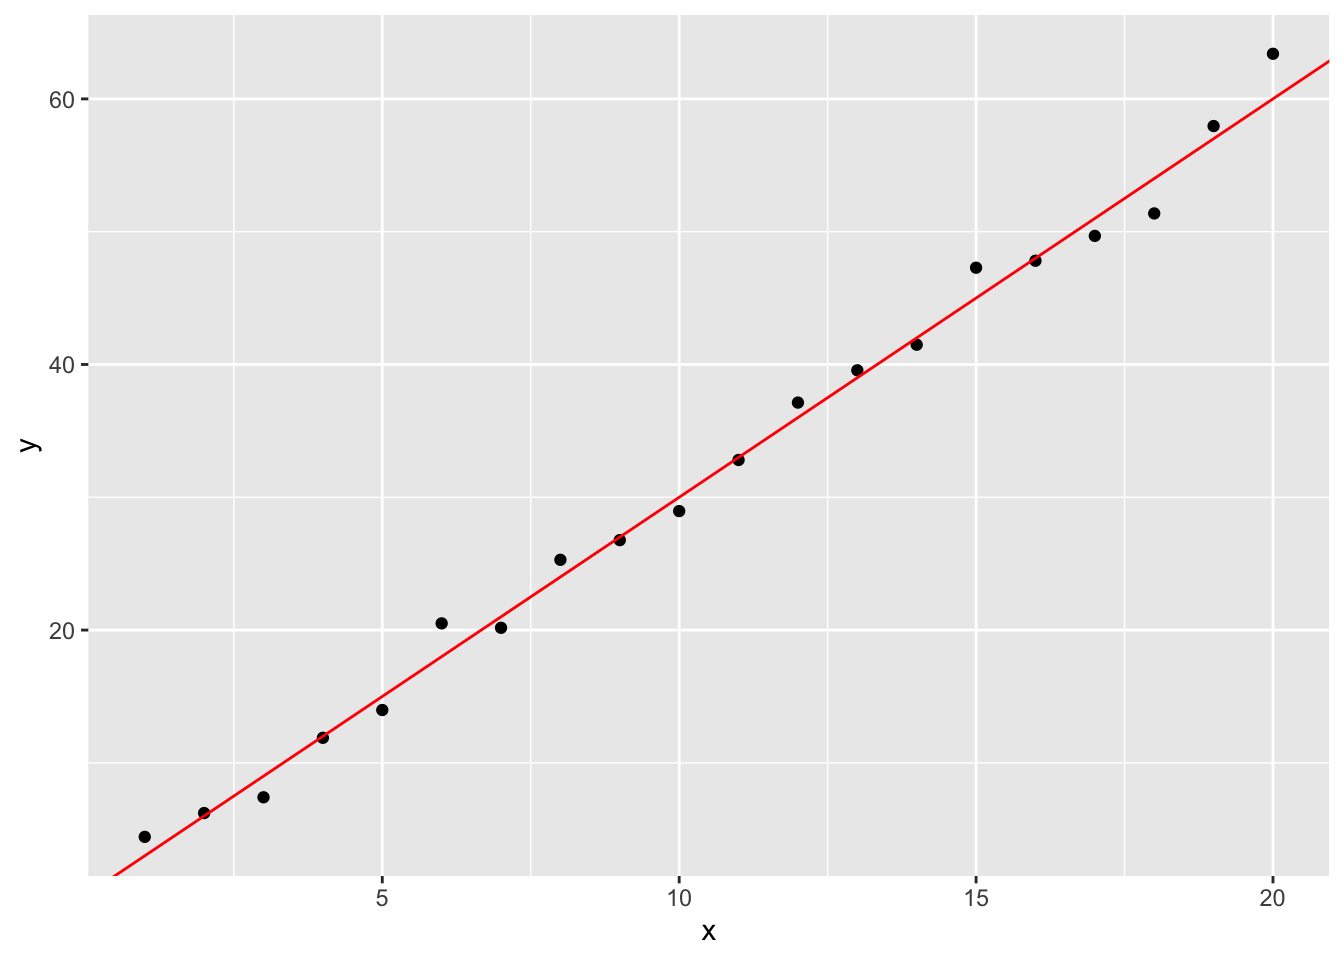
\includegraphics{smr_book_files/figure-latex/unnamed-chunk-41-1.pdf}

However, the \texttt{ggplot} library is now the new standard plotting library.
In ggplot, a plot is decomposed in three main components: data, coordinate
system and visual marks, called \emph{geoms}.
The plot is built by stacking up layers of visualization objects.
Data is in form of dataframes and the columns are selected in the aesthetics
arguments.

The same plot shown before can be drawn with ggplot in the following way.

\begin{Shaded}
\begin{Highlighting}[]
\FunctionTok{library}\NormalTok{(ggplot2)}
\NormalTok{gg\_df }\OtherTok{\textless{}{-}} \FunctionTok{tibble}\NormalTok{(}\AttributeTok{x =}\NormalTok{ x, }\AttributeTok{y =}\NormalTok{ y)}

\FunctionTok{ggplot}\NormalTok{(gg\_df) }\SpecialCharTok{+}
  \FunctionTok{geom\_point}\NormalTok{(}\AttributeTok{mapping =} \FunctionTok{aes}\NormalTok{(x, y)) }\SpecialCharTok{+}
  \FunctionTok{geom\_abline}\NormalTok{(}\AttributeTok{mapping =} \FunctionTok{aes}\NormalTok{(}\AttributeTok{intercept =} \DecValTok{0}\NormalTok{, }\AttributeTok{slope =} \DecValTok{3}\NormalTok{), }\AttributeTok{color =} \StringTok{"red"}\NormalTok{)}
\end{Highlighting}
\end{Shaded}

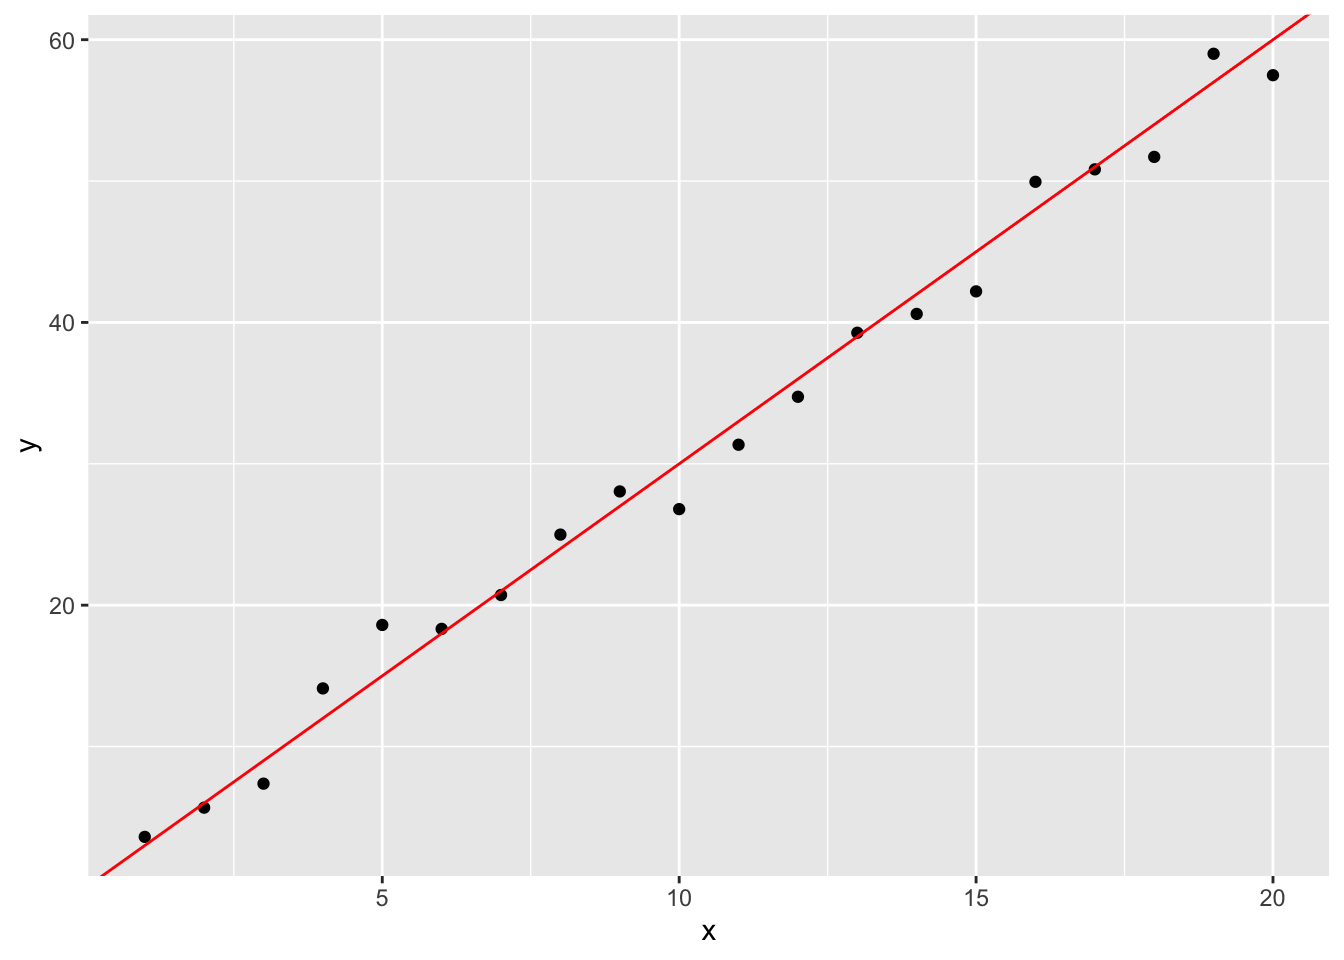
\includegraphics{smr_book_files/figure-latex/unnamed-chunk-42-1.pdf}

This is just a brief example. More will be seen in the next lessons.
Check out this
\href{https://github.com/rstudio/cheatsheets/blob/main/data-visualization.pdf}{cheatsheet}
for quick look-up on ggplot functions.

\section{Examples: plot and data manipulation}\label{examples-plot-and-data-manipulation}

Combining altogether, here a data visualization workflow on the
\href{https://www.gapminder.org/data/}{Gapminder} dataset.

\begin{Shaded}
\begin{Highlighting}[]
\FunctionTok{library}\NormalTok{(gapminder)}
\CommentTok{\# have a quick look at the Gapminder dataset}
\FunctionTok{str}\NormalTok{(gapminder)}
\end{Highlighting}
\end{Shaded}

\begin{verbatim}
## tibble [1,704 x 6] (S3: tbl_df/tbl/data.frame)
##  $ country  : Factor w/ 142 levels "Afghanistan",..: 1 1 1 1 1 1 1 1 1 1 ...
##  $ continent: Factor w/ 5 levels "Africa","Americas",..: 3 3 3 3 3 3 3 3 3 3 ...
##  $ year     : int [1:1704] 1952 1957 1962 1967 1972 1977 1982 1987 1992 1997 ...
##  $ lifeExp  : num [1:1704] 28.8 30.3 32 34 36.1 ...
##  $ pop      : int [1:1704] 8425333 9240934 10267083 11537966 13079460 14880372 12881816 13867957 16317921 22227415 ...
##  $ gdpPercap: num [1:1704] 779 821 853 836 740 ...
\end{verbatim}

A factor, which we haven't seen yet, is just a data-type characterizing a
discrete categorical variable; the levels of a factor describe how many
distinct categories it can take value from (e.g.~the variable \texttt{continent} takes
values from the set \texttt{\{Africa,\ Americas,\ Asia,\ Europe,\ Oceania\}}).

Let's say we want to compare the GDP per capita of some
different countries (Italy, Japan, Brasil and Ethiopia),
plotted against time (year by year).

\begin{Shaded}
\begin{Highlighting}[]
\CommentTok{\# transform the dataset according to what is necessary}
\NormalTok{wanted\_countries }\OtherTok{\textless{}{-}} \FunctionTok{c}\NormalTok{(}\StringTok{"Italy"}\NormalTok{, }\StringTok{"Japan"}\NormalTok{, }\StringTok{"Brazil"}\NormalTok{, }\StringTok{"Ethiopia"}\NormalTok{)}
\NormalTok{gapminder }\SpecialCharTok{\%\textgreater{}\%}
\NormalTok{  dplyr}\SpecialCharTok{::}\FunctionTok{filter}\NormalTok{(country }\SpecialCharTok{\%in\%}\NormalTok{ wanted\_countries) }\SpecialCharTok{\%\textgreater{}\%}
  \CommentTok{\# now feed the filtered data to ggplot (using the pipe op)}
  \FunctionTok{ggplot}\NormalTok{() }\SpecialCharTok{+}
    \FunctionTok{geom\_line}\NormalTok{(}\FunctionTok{aes}\NormalTok{(year, gdpPercap, }\AttributeTok{color =}\NormalTok{ country))}
\end{Highlighting}
\end{Shaded}

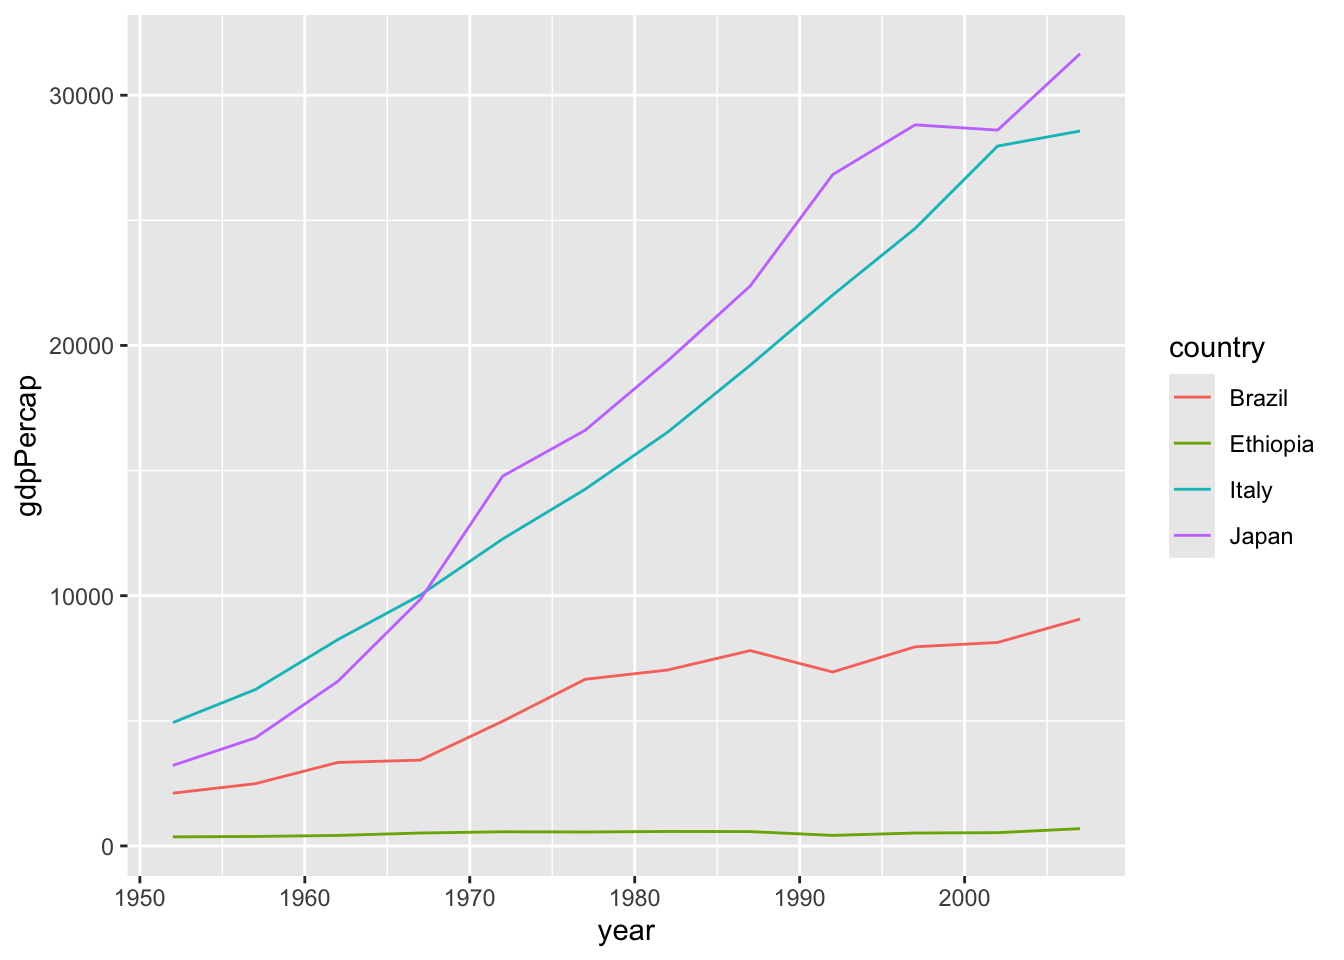
\includegraphics{smr_book_files/figure-latex/unnamed-chunk-44-1.pdf}

If we want to add some information about the same measure over the whole
continent, showing for instance the boundaries of GDP among all countries
in the same continent of the four selected countries, this
is more or less what we can do

\begin{Shaded}
\begin{Highlighting}[]
\CommentTok{\# give all the data to ggplot, we\textquotesingle{}ll filter later}
\NormalTok{plt }\OtherTok{\textless{}{-}}\NormalTok{ gapminder }\SpecialCharTok{\%\textgreater{}\%}
  \FunctionTok{ggplot}\NormalTok{() }\SpecialCharTok{+}
    \FunctionTok{geom\_line}\NormalTok{(}\AttributeTok{data =}\NormalTok{ . }\SpecialCharTok{\%\textgreater{}\%}
\NormalTok{      dplyr}\SpecialCharTok{::}\FunctionTok{filter}\NormalTok{(country }\SpecialCharTok{\%in\%}\NormalTok{ wanted\_countries),}
              \FunctionTok{aes}\NormalTok{(year, gdpPercap, }\AttributeTok{color =}\NormalTok{ country)) }\SpecialCharTok{+}
    \CommentTok{\# now group by continent and get the upper/lower bounds}
    \FunctionTok{geom\_ribbon}\NormalTok{(}\AttributeTok{data =}\NormalTok{ . }\SpecialCharTok{\%\textgreater{}\%}
      \CommentTok{\# min(NA) = NA, make sure NAs are excluded}
\NormalTok{      dplyr}\SpecialCharTok{::}\FunctionTok{filter}\NormalTok{(}\SpecialCharTok{!}\FunctionTok{is.na}\NormalTok{(gdpPercap)) }\SpecialCharTok{\%\textgreater{}\%}
      \CommentTok{\# gather all entries for each continent separately}
\NormalTok{      dplyr}\SpecialCharTok{::}\FunctionTok{group\_by}\NormalTok{(continent, year) }\SpecialCharTok{\%\textgreater{}\%}
      \CommentTok{\# compute aggregated quantity (min/max)}
\NormalTok{      dplyr}\SpecialCharTok{::}\FunctionTok{summarize}\NormalTok{(}\AttributeTok{minGdp =} \FunctionTok{min}\NormalTok{(gdpPercap),}
                       \AttributeTok{maxGdp =} \FunctionTok{max}\NormalTok{(gdpPercap), }\FunctionTok{across}\NormalTok{()) }\SpecialCharTok{\%\textgreater{}\%}
\NormalTok{      dplyr}\SpecialCharTok{::}\FunctionTok{filter}\NormalTok{(country }\SpecialCharTok{\%in\%}\NormalTok{ wanted\_countries),}
              \FunctionTok{aes}\NormalTok{(}\AttributeTok{ymin =}\NormalTok{ minGdp, }\AttributeTok{ymax =}\NormalTok{ maxGdp,}
                  \AttributeTok{x =}\NormalTok{ year, }\AttributeTok{color =}\NormalTok{ country, }\AttributeTok{fill =}\NormalTok{ country),}
              \AttributeTok{alpha =} \FloatTok{0.1}\NormalTok{, }\AttributeTok{linetype =} \StringTok{"dashed"}\NormalTok{, }\AttributeTok{size =} \FloatTok{0.2}\NormalTok{)}
\end{Highlighting}
\end{Shaded}

\begin{verbatim}
## Warning: Using `size` aesthetic for lines was deprecated in ggplot2 3.4.0.
## i Please use `linewidth` instead.
## This warning is displayed once every 8 hours.
## Call `lifecycle::last_lifecycle_warnings()` to see where this warning was
## generated.
\end{verbatim}

\begin{Shaded}
\begin{Highlighting}[]
\NormalTok{plt}
\end{Highlighting}
\end{Shaded}

\begin{verbatim}
## Warning: There was 1 warning in `dplyr::summarize()`.
## i In argument: `across()`.
## Caused by warning:
## ! Using `across()` without supplying `.cols` was deprecated in dplyr 1.1.0.
## i Please supply `.cols` instead.
\end{verbatim}

\begin{verbatim}
## Warning: Returning more (or less) than 1 row per `summarise()` group was deprecated in
## dplyr 1.1.0.
## i Please use `reframe()` instead.
## i When switching from `summarise()` to `reframe()`, remember that `reframe()`
##   always returns an ungrouped data frame and adjust accordingly.
## Call `lifecycle::last_lifecycle_warnings()` to see where this warning was
## generated.
\end{verbatim}

\begin{verbatim}
## `summarise()` has grouped output by 'continent', 'year'. You can override using
## the `.groups` argument.
\end{verbatim}

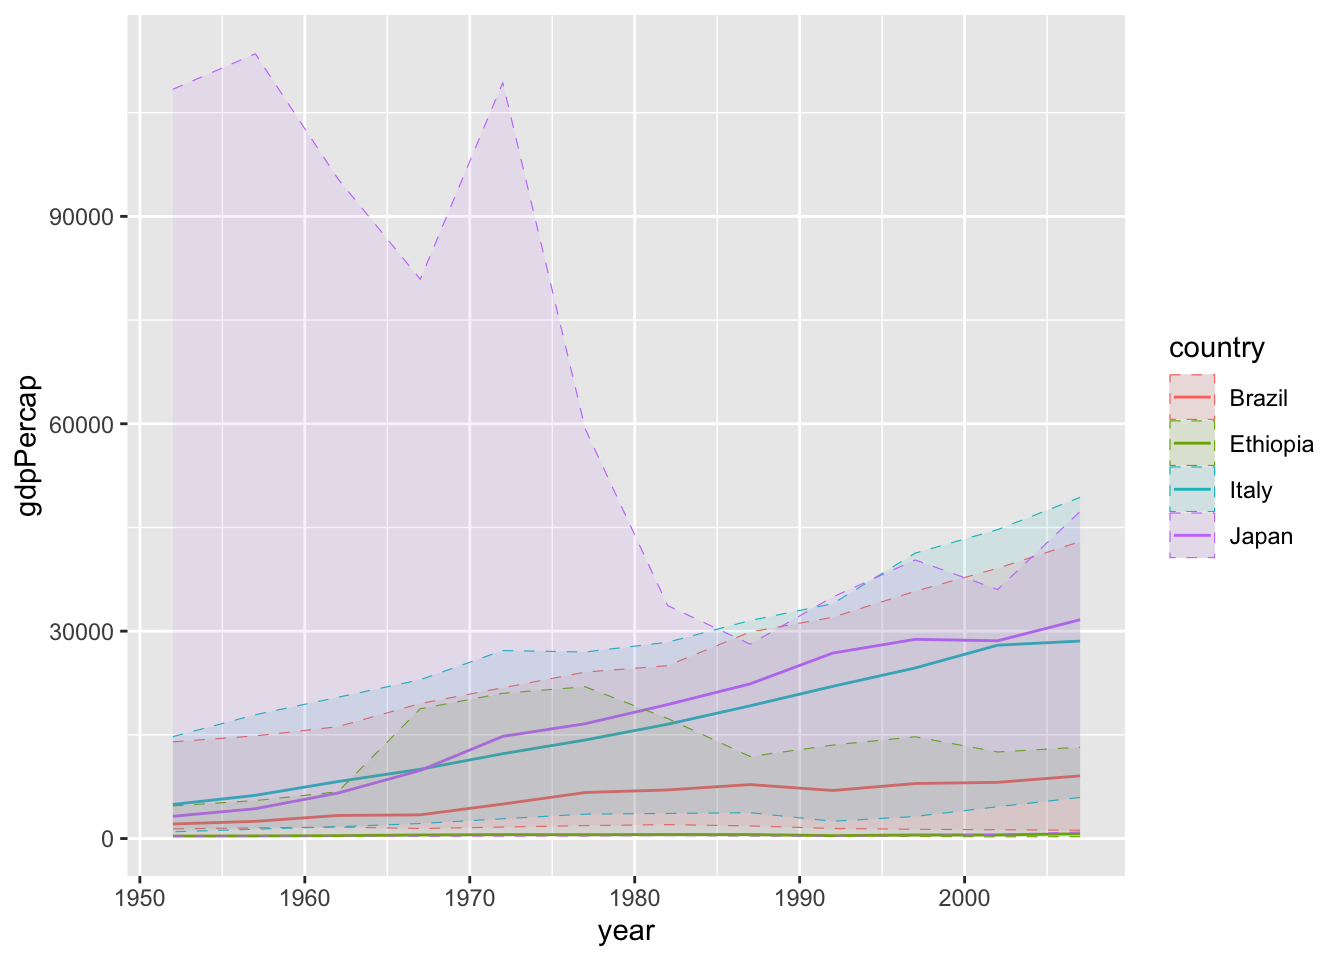
\includegraphics{smr_book_files/figure-latex/unnamed-chunk-45-1.pdf}
But, since it looks a bit confusing, we might want four separate plots.

\begin{Shaded}
\begin{Highlighting}[]
\NormalTok{wanted\_continents }\OtherTok{\textless{}{-}}\NormalTok{ gapminder }\SpecialCharTok{\%\textgreater{}\%}
\NormalTok{  dplyr}\SpecialCharTok{::}\FunctionTok{filter}\NormalTok{(country }\SpecialCharTok{\%in\%}\NormalTok{ wanted\_countries) }\SpecialCharTok{\%\textgreater{}\%}
  \CommentTok{\# extract one column from a dataframe (different from select)}
\NormalTok{  dplyr}\SpecialCharTok{::}\FunctionTok{pull}\NormalTok{(continent) }\SpecialCharTok{\%\textgreater{}\%}
  \FunctionTok{unique}\NormalTok{()}

\NormalTok{gapminder }\SpecialCharTok{\%\textgreater{}\%}
\NormalTok{  dplyr}\SpecialCharTok{::}\FunctionTok{filter}\NormalTok{(continent }\SpecialCharTok{\%in\%}\NormalTok{ wanted\_continents) }\SpecialCharTok{\%\textgreater{}\%}
  \FunctionTok{ggplot}\NormalTok{() }\SpecialCharTok{+}
    \FunctionTok{geom\_line}\NormalTok{(}\AttributeTok{data =}\NormalTok{ . }\SpecialCharTok{\%\textgreater{}\%}
\NormalTok{      dplyr}\SpecialCharTok{::}\FunctionTok{filter}\NormalTok{(country }\SpecialCharTok{\%in\%}\NormalTok{ wanted\_countries),}
              \FunctionTok{aes}\NormalTok{(year, gdpPercap, }\AttributeTok{color =}\NormalTok{ country)) }\SpecialCharTok{+}
    \CommentTok{\# now group by continent and get the upper/lower bounds}
    \FunctionTok{geom\_ribbon}\NormalTok{(}\AttributeTok{data =}\NormalTok{ . }\SpecialCharTok{\%\textgreater{}\%}
      \CommentTok{\# min(NA) = NA, make sure NAs are excluded}
\NormalTok{      dplyr}\SpecialCharTok{::}\FunctionTok{filter}\NormalTok{(}\SpecialCharTok{!}\FunctionTok{is.na}\NormalTok{(gdpPercap)) }\SpecialCharTok{\%\textgreater{}\%}
      \CommentTok{\# gather all entries for each continent separately}
\NormalTok{      dplyr}\SpecialCharTok{::}\FunctionTok{group\_by}\NormalTok{(continent, year) }\SpecialCharTok{\%\textgreater{}\%}
      \CommentTok{\# compute aggregated quantity (min/max)}
\NormalTok{      dplyr}\SpecialCharTok{::}\FunctionTok{summarize}\NormalTok{(}\AttributeTok{minGdp =} \FunctionTok{min}\NormalTok{(gdpPercap),}
                       \AttributeTok{maxGdp =} \FunctionTok{max}\NormalTok{(gdpPercap), }\FunctionTok{across}\NormalTok{()) }\SpecialCharTok{\%\textgreater{}\%}
\NormalTok{      dplyr}\SpecialCharTok{::}\FunctionTok{filter}\NormalTok{(country }\SpecialCharTok{\%in\%}\NormalTok{ wanted\_countries),}
              \FunctionTok{aes}\NormalTok{(}\AttributeTok{ymin =}\NormalTok{ minGdp, }\AttributeTok{ymax =}\NormalTok{ maxGdp,}
                  \AttributeTok{x =}\NormalTok{ year, }\AttributeTok{color =}\NormalTok{ country, }\AttributeTok{fill =}\NormalTok{ country),}
              \AttributeTok{alpha =} \FloatTok{0.1}\NormalTok{, }\AttributeTok{linetype =} \StringTok{"dashed"}\NormalTok{, }\AttributeTok{size =} \FloatTok{0.2}\NormalTok{) }\SpecialCharTok{+}
      \FunctionTok{facet\_wrap}\NormalTok{(}\FunctionTok{vars}\NormalTok{(continent)) }\SpecialCharTok{+}
      \FunctionTok{labs}\NormalTok{(}\AttributeTok{title =} \FunctionTok{paste}\NormalTok{(}\StringTok{"Country GDP per capita compared with"}\NormalTok{,}
           \StringTok{"continent lower and upper bounds"}\NormalTok{),}
           \AttributeTok{x =} \StringTok{"year"}\NormalTok{, }\AttributeTok{y =} \StringTok{"GDP per capita (PPP dollars)"}\NormalTok{)}
\end{Highlighting}
\end{Shaded}

\begin{verbatim}
## Warning: Returning more (or less) than 1 row per `summarise()` group was deprecated in
## dplyr 1.1.0.
## i Please use `reframe()` instead.
## i When switching from `summarise()` to `reframe()`, remember that `reframe()`
##   always returns an ungrouped data frame and adjust accordingly.
## Call `lifecycle::last_lifecycle_warnings()` to see where this warning was
## generated.
\end{verbatim}

\begin{verbatim}
## `summarise()` has grouped output by 'continent', 'year'. You can override using
## the `.groups` argument.
\end{verbatim}

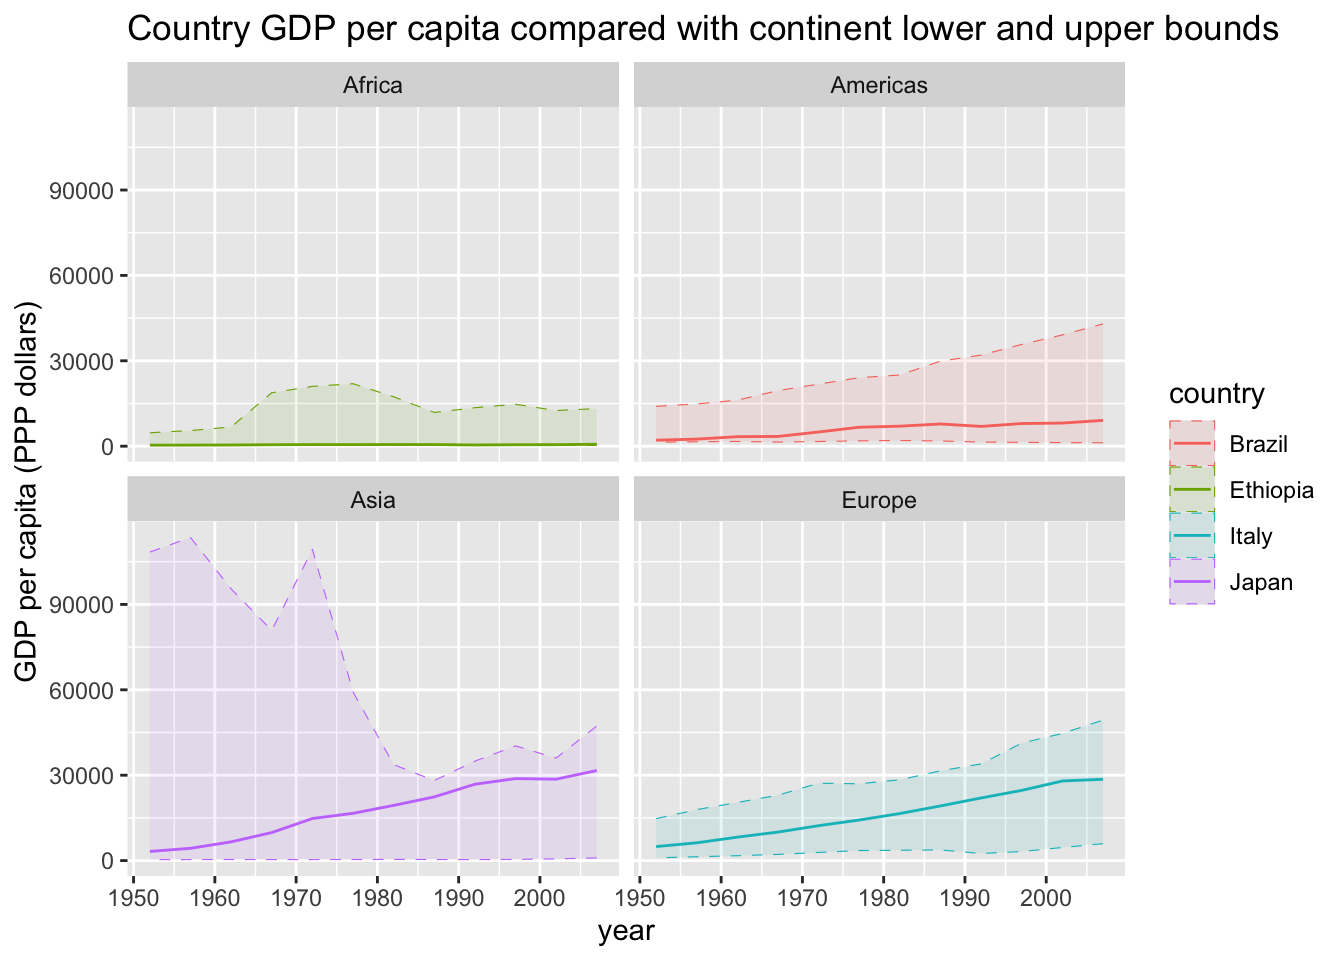
\includegraphics{smr_book_files/figure-latex/unnamed-chunk-46-1.pdf}

\section{Probability}\label{probability}

Base R provide functions to handle almost any probability distribution.
These functions are usually divided into four categories:

\begin{itemize}
\tightlist
\item
  density function
\item
  distribution function
\item
  quantile function
\item
  random function (sampling)
\end{itemize}

\begin{Shaded}
\begin{Highlighting}[]
\NormalTok{n }\OtherTok{\textless{}{-}} \DecValTok{10}
\NormalTok{normal\_samples }\OtherTok{\textless{}{-}} \FunctionTok{rnorm}\NormalTok{(}\AttributeTok{n =}\NormalTok{ n, }\AttributeTok{mean =} \DecValTok{0}\NormalTok{, }\AttributeTok{sd =} \DecValTok{1}\NormalTok{) }\CommentTok{\# sample 10 Gaussian samples}
\NormalTok{normal\_samples}
\end{Highlighting}
\end{Shaded}

\begin{verbatim}
##  [1] -1.2317960  0.3460598  1.3832943  0.7350193  0.7750545  1.2920892
##  [7] -1.8497872  1.0520194 -1.0308002  0.3268712
\end{verbatim}

\begin{Shaded}
\begin{Highlighting}[]
\CommentTok{\# compute the density function (over another Normal)}
\FunctionTok{dnorm}\NormalTok{(normal\_samples, }\AttributeTok{mean =} \DecValTok{2}\NormalTok{, }\AttributeTok{sd =} \DecValTok{1}\NormalTok{)}
\end{Highlighting}
\end{Shaded}

\begin{verbatim}
##  [1] 0.0021523581 0.1016014415 0.3298552116 0.1792405408 0.1884006912
##  [6] 0.3105198758 0.0002413242 0.2545464068 0.0040387767 0.0984094475
\end{verbatim}

\begin{Shaded}
\begin{Highlighting}[]
\CommentTok{\# cumulative distribution function}
\FunctionTok{pnorm}\NormalTok{(normal\_samples, }\AttributeTok{mean =} \DecValTok{0}\NormalTok{, }\AttributeTok{sd =} \DecValTok{1}\NormalTok{)}
\end{Highlighting}
\end{Shaded}

\begin{verbatim}
##  [1] 0.10901265 0.63535113 0.91671268 0.76883614 0.78084628 0.90183688
##  [7] 0.03217211 0.85360468 0.15131727 0.62811736
\end{verbatim}

\begin{Shaded}
\begin{Highlighting}[]
\CommentTok{\# get the quantiles of a normal}
\FunctionTok{qnorm}\NormalTok{(}\FunctionTok{c}\NormalTok{(}\FloatTok{0.05}\NormalTok{, }\FloatTok{0.95}\NormalTok{), }\AttributeTok{mean =} \DecValTok{0}\NormalTok{, }\AttributeTok{sd =} \DecValTok{1}\NormalTok{)}
\end{Highlighting}
\end{Shaded}

\begin{verbatim}
## [1] -1.644854  1.644854
\end{verbatim}

\section{Extras}\label{extras}

\subsection{File system and helper}\label{file-system-and-helper}

R language provides several tools for management of files and function help.
Here some useful console commands. Note that most of them are also available
on RStudio through the graphic interface (buttons).

R saves all the variables and you can display them with \texttt{ls()}.

\begin{Shaded}
\begin{Highlighting}[]
\FunctionTok{rm}\NormalTok{(}\AttributeTok{list =} \FunctionTok{ls}\NormalTok{()) }\CommentTok{\# clear up the space removing all variables stored so far}
\CommentTok{\# let\textquotesingle{}s add some variables}
\NormalTok{x }\OtherTok{\textless{}{-}} \DecValTok{1}\SpecialCharTok{:}\DecValTok{10}
\NormalTok{y }\OtherTok{\textless{}{-}}\NormalTok{ x[x }\SpecialCharTok{\%\%} \DecValTok{2} \SpecialCharTok{==} \DecValTok{0}\NormalTok{]}

\FunctionTok{ls}\NormalTok{() }\CommentTok{\# check variables in the environment}
\end{Highlighting}
\end{Shaded}

\begin{verbatim}
## [1] "x" "y"
\end{verbatim}

The working directory is the folder located on your computer from which R
navigates the filesystem.

\begin{Shaded}
\begin{Highlighting}[]
\FunctionTok{getwd}\NormalTok{() }\CommentTok{\# check your wd}
\end{Highlighting}
\end{Shaded}

\begin{verbatim}
## [1] "/Users/runner/work/statistical-models-r/statistical-models-r"
\end{verbatim}

\begin{Shaded}
\begin{Highlighting}[]
\FunctionTok{setwd}\NormalTok{(}\StringTok{"./tmp"}\NormalTok{) }\CommentTok{\# set the working directory to an arbitrary (existing) folder}
\CommentTok{\# save the current environment}
\FunctionTok{save.image}\NormalTok{(}\StringTok{"./01\_test.RData"}\NormalTok{)}
\CommentTok{\# check that it\textquotesingle{}s on the working directory}
\FunctionTok{dir}\NormalTok{()}
\end{Highlighting}
\end{Shaded}

RStudio typically save the environment automatically,
but sometimes (if not every time you close R) you should
clear the environment variables, because loading many variables
when opening RStudio might fill up too much memory.

You can also read function helpers simply by typing \texttt{?function\_name}. This
will open a formatted page with information about a specific R function or object.

\begin{Shaded}
\begin{Highlighting}[]
\NormalTok{?quit }\CommentTok{\# help for the quit function}

\NormalTok{?Arithmetic }\CommentTok{\# help for more general syntax information}
\FunctionTok{help}\NormalTok{(Trig) }\CommentTok{\# or use help(name)}
\end{Highlighting}
\end{Shaded}

\subsection{Packages}\label{packages}

Packages can be installed via command line using
\texttt{install.packages("package\_name")}, or through RStudio graphical interface.

\begin{Shaded}
\begin{Highlighting}[]
\CommentTok{\# the following function call is commented because package installation should}
\CommentTok{\# not be included in a script (but you can find it commented, showing that the}
\CommentTok{\# script requires a package as dependency)}

\CommentTok{\# install.packages("tidyverse")}
\end{Highlighting}
\end{Shaded}

And then you can load the package with \texttt{library}.

\begin{Shaded}
\begin{Highlighting}[]
\FunctionTok{library}\NormalTok{(tidyverse)}
\end{Highlighting}
\end{Shaded}

\begin{verbatim}
## -- Attaching core tidyverse packages ------------------------ tidyverse 2.0.0 --
## v forcats   1.0.0     v readr     2.1.5
## v lubridate 1.9.3     v stringr   1.5.1
## v purrr     1.0.2     v tidyr     1.3.1
## -- Conflicts ------------------------------------------ tidyverse_conflicts() --
## x dplyr::filter() masks stats::filter()
## x dplyr::lag()    masks stats::lag()
## i Use the conflicted package (<http://conflicted.r-lib.org/>) to force all conflicts to become errors
\end{verbatim}

\subsection{Arrow sign}\label{arrow-sign}

The difference between \texttt{\textless{}-} and \texttt{=} is not just programming \emph{style} preference.
Here an example where using \texttt{=} rather than \texttt{\textless{}-} makes a difference:

\begin{Shaded}
\begin{Highlighting}[]
\CommentTok{\# gives error: argument \textquotesingle{}b\textquotesingle{} is not part of \textquotesingle{}within\textquotesingle{}}
\FunctionTok{within}\NormalTok{(}\FunctionTok{data.frame}\NormalTok{(}\AttributeTok{a =} \FunctionTok{rnorm}\NormalTok{(}\DecValTok{2}\NormalTok{)), }\AttributeTok{b =}\NormalTok{ a}\SpecialCharTok{\^{}}\DecValTok{2}\NormalTok{)}
\end{Highlighting}
\end{Shaded}

\begin{verbatim}
## Error in eval(substitute(expr), e): argument is missing, with no default
\end{verbatim}

\begin{Shaded}
\begin{Highlighting}[]
\CommentTok{\# \textquotesingle{}b\textless{}{-}a\^{}2\textquotesingle{} is the value passed to the expr argument of within()}
\FunctionTok{within}\NormalTok{(}\FunctionTok{data.frame}\NormalTok{(}\AttributeTok{a =} \FunctionTok{rnorm}\NormalTok{(}\DecValTok{2}\NormalTok{)), b }\OtherTok{\textless{}{-}}\NormalTok{ a}\SpecialCharTok{\^{}}\DecValTok{2}\NormalTok{)}
\end{Highlighting}
\end{Shaded}

\begin{verbatim}
##            a         b
## 1 -0.8079864 0.6528421
## 2  1.9477103 3.7935752
\end{verbatim}

Although this event might never occur in one's programming experience, it's
safer (and more elegant) to use \texttt{\textless{}-} when assigning variable.

Besides, \texttt{-\textgreater{}} is also valid and it is used (more intuitive) when assigning pipes
result to variables.

\begin{Shaded}
\begin{Highlighting}[]
\FunctionTok{library}\NormalTok{(dplyr)}

\NormalTok{x }\OtherTok{\textless{}{-}}\NormalTok{ starwars }\SpecialCharTok{\%\textgreater{}\%}
\NormalTok{  dplyr}\SpecialCharTok{::}\FunctionTok{mutate}\NormalTok{(}\AttributeTok{bmi =}\NormalTok{ mass }\SpecialCharTok{/}\NormalTok{ ((height }\SpecialCharTok{/} \DecValTok{100}\NormalTok{) }\SpecialCharTok{\^{}} \DecValTok{2}\NormalTok{)) }\SpecialCharTok{\%\textgreater{}\%}
\NormalTok{  dplyr}\SpecialCharTok{::}\FunctionTok{filter}\NormalTok{(}\SpecialCharTok{!}\FunctionTok{is.na}\NormalTok{(bmi)) }\SpecialCharTok{\%\textgreater{}\%}
\NormalTok{  dplyr}\SpecialCharTok{::}\FunctionTok{group\_by}\NormalTok{(species) }\SpecialCharTok{\%\textgreater{}\%}
\NormalTok{  dplyr}\SpecialCharTok{::}\FunctionTok{summarise}\NormalTok{(}\AttributeTok{bmi =} \FunctionTok{mean}\NormalTok{(bmi)) }\SpecialCharTok{\%\textgreater{}\%}
\NormalTok{  dplyr}\SpecialCharTok{::}\FunctionTok{arrange}\NormalTok{(}\FunctionTok{desc}\NormalTok{(bmi))}

\NormalTok{x}
\end{Highlighting}
\end{Shaded}

\begin{verbatim}
## # A tibble: 32 x 2
##    species          bmi
##    <chr>          <dbl>
##  1 Hutt           443. 
##  2 Vulptereen      50.9
##  3 Yoda's species  39.0
##  4 Kaleesh         34.1
##  5 Droid           32.7
##  6 Dug             31.9
##  7 Trandoshan      31.3
##  8 Sullustan       26.6
##  9 Zabrak          26.1
## 10 Besalisk        26.0
## # i 22 more rows
\end{verbatim}

\section{Exercises}\label{exercises}

\begin{enumerate}
\def\labelenumi{\arabic{enumi}.}
\tightlist
\item
  LogSumExp trick
\end{enumerate}

Try to implement the log-sum-exp trick in a function that takes as argument
three \texttt{numeric} variables and computed the log of the sum of the exponentials
in a numerically stable way.
See this
\href{https://en.wikipedia.org/wiki/LogSumExp\#log-sum-exp_trick_for_log-domain_calculations}{Wiki paragraph}
if you don't know the trick yet.

\begin{Shaded}
\begin{Highlighting}[]
\NormalTok{log\_sum\_exp3 }\OtherTok{\textless{}{-}} \ControlFlowTok{function}\NormalTok{(a, b, c) \{}
  \CommentTok{\# delete this function and re{-}write it using the trick}
  \CommentTok{\# in order to make it work}
  \FunctionTok{return}\NormalTok{(}\FunctionTok{log}\NormalTok{(}\FunctionTok{exp}\NormalTok{(a) }\SpecialCharTok{+} \FunctionTok{exp}\NormalTok{(b) }\SpecialCharTok{+} \FunctionTok{exp}\NormalTok{(c)))}
\NormalTok{\}}

\CommentTok{\# test {-} this result is obviously wrong: edit the function above}
\FunctionTok{log\_sum\_exp3}\NormalTok{(}\AttributeTok{a =} \SpecialCharTok{{-}}\DecValTok{1000}\NormalTok{, }\AttributeTok{b =} \SpecialCharTok{{-}}\DecValTok{1001}\NormalTok{, }\AttributeTok{c =} \SpecialCharTok{{-}}\DecValTok{999}\NormalTok{) }\CommentTok{\# should give {-}998.5924}
\end{Highlighting}
\end{Shaded}

\begin{verbatim}
## [1] -Inf
\end{verbatim}

\chapter{Some elementary statistics problems}\label{some-elementary-statistics-problems}

In the following paragraphs, we will see some applications of the R
software to solve elementary statistics problems.

\section{Hypothesis testing}\label{hypothesis-testing}

\subsection{Example}\label{example}

The rector of Politecnico di Torino wants to monitor the spread of Covid-19
virus inside the university, to check whether it is in line with the overall
diffusion on the Italian territory, or whether it is higher,
and therefore requires extra safety measures.

Tests are made on a sample of \(n = 250\) students out of the total \(N = 5000\)
students (because of whatever reasons, such as economic or sustainability
concerns). We assume that the tests are \emph{perfect}, meaning that they have
\(100\%\) sensitivity (true positive rate) and specificity (true negative rate).

We know that \(p_0 = 0.015\) is the prevalence of the virus in the Italian
population at the end of 2021, and we are given a \emph{warning} threshold for the
prevalence of \(p_1 = 0.04\), above which the rector will have reasons to adopt
more restrictive measures.

\subsection{False alarm}\label{false-alarm}

\begin{quote}
\textbf{Question}: given a threshold \(x_0\) of positive tests, what are the false
alarm and the false non-alarm probabilities?
\end{quote}

Formally, a false alarm (type I error) probability is defined as
the probability of the r.v. counting the positive tests \(X\) being greater than
or equal to the threshold \(x_0\), conditioned on the fact that the prevalence
is not different than the Italian reference value \(p_0\). I.e.

\[
P(X \geq x_0 | p = p_0)
\]
Recall that \(X \sim \text{Hypergeometric}(N, K, n)\) where \(p = K/N\).

The pmf is the following

\[
P(X = x) = \frac{\binom{K}{x}\binom{N - K}{n - x}}{\binom{N}{n}}\,,
\]
which leads to the false alarm probability computation

\[
P(X \geq x_0 | p = p_0) = \sum_{k = x_0}^{n}P(X = k) = \sum_{k = x_0}^{n}\frac{\binom{K}{k}
\binom{N - K}{n - k}}{\binom{N}{n}}\,.
\]

When \(N\) is large enough and \(p\) small enough, we can use the Binomial
approximation. To be clear, with such approximation,
we assume that while sampling from the population, the proportion of positives
stays the same (which in our case it is safe to assume).

Therefore we approximate the false alarm probability with

\[
P(X \geq x_0 | p = p_0) = \alpha \approx \sum_{k = x_0}^{n}{\binom{n}{k}}p^{k}(1-p)^{n-k}\,.
\]

Similarly, we compute the false non-alarm probability (type II error), defined
as the probability of the r.v. counting the positive tests \(X\) being lower than
the threshold \(x_0\), conditioned on the fact that the prevalence is the one we
identified as worrying, i.e.~\(p = p_1\).

\[
P(X < x_0 | p = p_1) = \beta \approx \sum_{k = 0}^{x_0 - 1}{\binom{n}{k}}p^{k}(1-p)^{n-k}\,.
\]
To answer the question, let's now compute these quantities using the R functions
\texttt{phyper} and \texttt{pbinom}. We can do this for several values of \(x_0\) i.e.
\(\forall x_0 \in \{1, \dots, 10\}\) so to understand how \(\alpha\) and \(\beta\) change.

\begin{Shaded}
\begin{Highlighting}[]
\CommentTok{\# import the main libraries}
\FunctionTok{library}\NormalTok{(tidyverse)}
\end{Highlighting}
\end{Shaded}

\begin{Shaded}
\begin{Highlighting}[]
\CommentTok{\# set random seed for reproducibility}
\FunctionTok{set.seed}\NormalTok{(}\DecValTok{42}\NormalTok{)}

\CommentTok{\# define the parameters of the test}
\NormalTok{N }\OtherTok{\textless{}{-}} \DecValTok{5000}
\NormalTok{n }\OtherTok{\textless{}{-}} \DecValTok{250}
\NormalTok{p0 }\OtherTok{\textless{}{-}}\NormalTok{ .}\DecValTok{015}
\NormalTok{p1 }\OtherTok{\textless{}{-}}\NormalTok{ .}\DecValTok{04}

\CommentTok{\# get the lower integer part in case the product is not natural}
\NormalTok{K0 }\OtherTok{\textless{}{-}} \FunctionTok{floor}\NormalTok{(N }\SpecialCharTok{*}\NormalTok{ p0)}
\NormalTok{K1 }\OtherTok{\textless{}{-}} \FunctionTok{floor}\NormalTok{(N }\SpecialCharTok{*}\NormalTok{ p1)}

\CommentTok{\# false positive (check phyper params with ?phyper)}
\CommentTok{\# we subtract 1 to x0 because we are looking for P(X \textgreater{}= x0) = 1 {-} P(X \textless{} x0{-}1),}
\CommentTok{\# not P(X \textgreater{} x0)}
\NormalTok{fp\_df }\OtherTok{\textless{}{-}} \FunctionTok{tibble}\NormalTok{(}
  \AttributeTok{x0 =} \DecValTok{1}\SpecialCharTok{:}\DecValTok{10}\NormalTok{,}
  \AttributeTok{hyp =} \DecValTok{1} \SpecialCharTok{{-}} \FunctionTok{phyper}\NormalTok{(x0 }\SpecialCharTok{{-}} \DecValTok{1}\NormalTok{, K0, N }\SpecialCharTok{{-}}\NormalTok{ K0, n),}
  \AttributeTok{bin =} \DecValTok{1} \SpecialCharTok{{-}} \FunctionTok{pbinom}\NormalTok{(x0 }\SpecialCharTok{{-}} \DecValTok{1}\NormalTok{, n, p0)}
\NormalTok{)}
\CommentTok{\# let\textquotesingle{}s view the result}
\NormalTok{fp\_df}
\end{Highlighting}
\end{Shaded}

\begin{verbatim}
## # A tibble: 10 x 3
##       x0     hyp     bin
##    <int>   <dbl>   <dbl>
##  1     1 0.979   0.977  
##  2     2 0.896   0.890  
##  3     3 0.732   0.725  
##  4     4 0.521   0.517  
##  5     5 0.321   0.322  
##  6     6 0.171   0.176  
##  7     7 0.0795  0.0847 
##  8     8 0.0325  0.0364 
##  9     9 0.0118  0.0141 
## 10    10 0.00382 0.00494
\end{verbatim}

\begin{Shaded}
\begin{Highlighting}[]
\CommentTok{\# false negative}
\CommentTok{\# again, we subtract 1: P(X \textless{} x0) = P(X \textless{}= x0{-}1) and}
\CommentTok{\# pbinom(x, n, p) := P(X \textless{}= x; n, p)}
\NormalTok{fn\_df }\OtherTok{\textless{}{-}} \FunctionTok{tibble}\NormalTok{(}
  \AttributeTok{x0 =} \DecValTok{1}\SpecialCharTok{:}\DecValTok{10}\NormalTok{,}
  \AttributeTok{hyp =} \FunctionTok{phyper}\NormalTok{(x0 }\SpecialCharTok{{-}} \DecValTok{1}\NormalTok{, K1, N }\SpecialCharTok{{-}}\NormalTok{ K1, n),}
  \AttributeTok{bin =} \FunctionTok{pbinom}\NormalTok{(x0 }\SpecialCharTok{{-}} \DecValTok{1}\NormalTok{, n, p1)}
\NormalTok{)}
\NormalTok{fn\_df}
\end{Highlighting}
\end{Shaded}

\begin{verbatim}
## # A tibble: 10 x 3
##       x0       hyp       bin
##    <int>     <dbl>     <dbl>
##  1     1 0.0000283 0.0000370
##  2     2 0.000339  0.000422 
##  3     3 0.00203   0.00242  
##  4     4 0.00810   0.00930  
##  5     5 0.0243    0.0270   
##  6     6 0.0587    0.0633   
##  7     7 0.119     0.125    
##  8     8 0.208     0.215    
##  9     9 0.322     0.328    
## 10    10 0.452     0.455
\end{verbatim}

We observe that with \(x_0 = 7\) we have
\[
\alpha = 0.0795,  \beta = 0.119
\]
which jointly optimize the two probabilities.
In order to get a more complete overview, we could plot those values together

\begin{Shaded}
\begin{Highlighting}[]
\FunctionTok{library}\NormalTok{(scales) }\CommentTok{\# to define custom scale on axes}
\end{Highlighting}
\end{Shaded}

\begin{Shaded}
\begin{Highlighting}[]
\CommentTok{\# join the two dataframes}
\NormalTok{tot\_df }\OtherTok{\textless{}{-}} \FunctionTok{left\_join}\NormalTok{(fp\_df, fn\_df,}
  \AttributeTok{by =} \StringTok{"x0"}\NormalTok{, }\AttributeTok{suffix =} \FunctionTok{c}\NormalTok{(}\StringTok{"alpha"}\NormalTok{, }\StringTok{"beta"}\NormalTok{)}
\NormalTok{)}
\NormalTok{tot\_df }\SpecialCharTok{\%\textgreater{}\%}
  \FunctionTok{ggplot}\NormalTok{() }\SpecialCharTok{+}
  \FunctionTok{geom\_bar}\NormalTok{(}\FunctionTok{aes}\NormalTok{(x0, hypalpha, }\AttributeTok{fill =} \StringTok{"alpha"}\NormalTok{), }\AttributeTok{alpha =}\NormalTok{ .}\DecValTok{3}\NormalTok{, }\AttributeTok{stat =} \StringTok{"identity"}\NormalTok{) }\SpecialCharTok{+}
  \FunctionTok{geom\_bar}\NormalTok{(}\FunctionTok{aes}\NormalTok{(x0, hypbeta, }\AttributeTok{fill =} \StringTok{"beta"}\NormalTok{), }\AttributeTok{alpha =}\NormalTok{ .}\DecValTok{3}\NormalTok{, }\AttributeTok{stat =} \StringTok{"identity"}\NormalTok{) }\SpecialCharTok{+}
  \FunctionTok{geom\_smooth}\NormalTok{(}\FunctionTok{aes}\NormalTok{(x0, binalpha, }\AttributeTok{color =} \StringTok{"alpha"}\NormalTok{), }\AttributeTok{se =} \ConstantTok{FALSE}\NormalTok{) }\SpecialCharTok{+}
  \FunctionTok{geom\_smooth}\NormalTok{(}\FunctionTok{aes}\NormalTok{(x0, binbeta, }\AttributeTok{color =} \StringTok{"beta"}\NormalTok{), }\AttributeTok{se =} \ConstantTok{FALSE}\NormalTok{) }\SpecialCharTok{+}
  \FunctionTok{labs}\NormalTok{(}\AttributeTok{x =} \StringTok{"thresh"}\NormalTok{, }\AttributeTok{y =} \StringTok{"prob"}\NormalTok{, }\AttributeTok{fill =} \StringTok{"hyper"}\NormalTok{, }\AttributeTok{color =} \StringTok{"binom"}\NormalTok{) }\SpecialCharTok{+}
  \CommentTok{\# print integers on the x axis}
  \FunctionTok{scale\_x\_continuous}\NormalTok{(}\AttributeTok{breaks =} \FunctionTok{pretty\_breaks}\NormalTok{(}\DecValTok{10}\NormalTok{))}
\end{Highlighting}
\end{Shaded}

\begin{verbatim}
## `geom_smooth()` using method = 'loess' and formula = 'y ~ x'
## `geom_smooth()` using method = 'loess' and formula = 'y ~ x'
\end{verbatim}

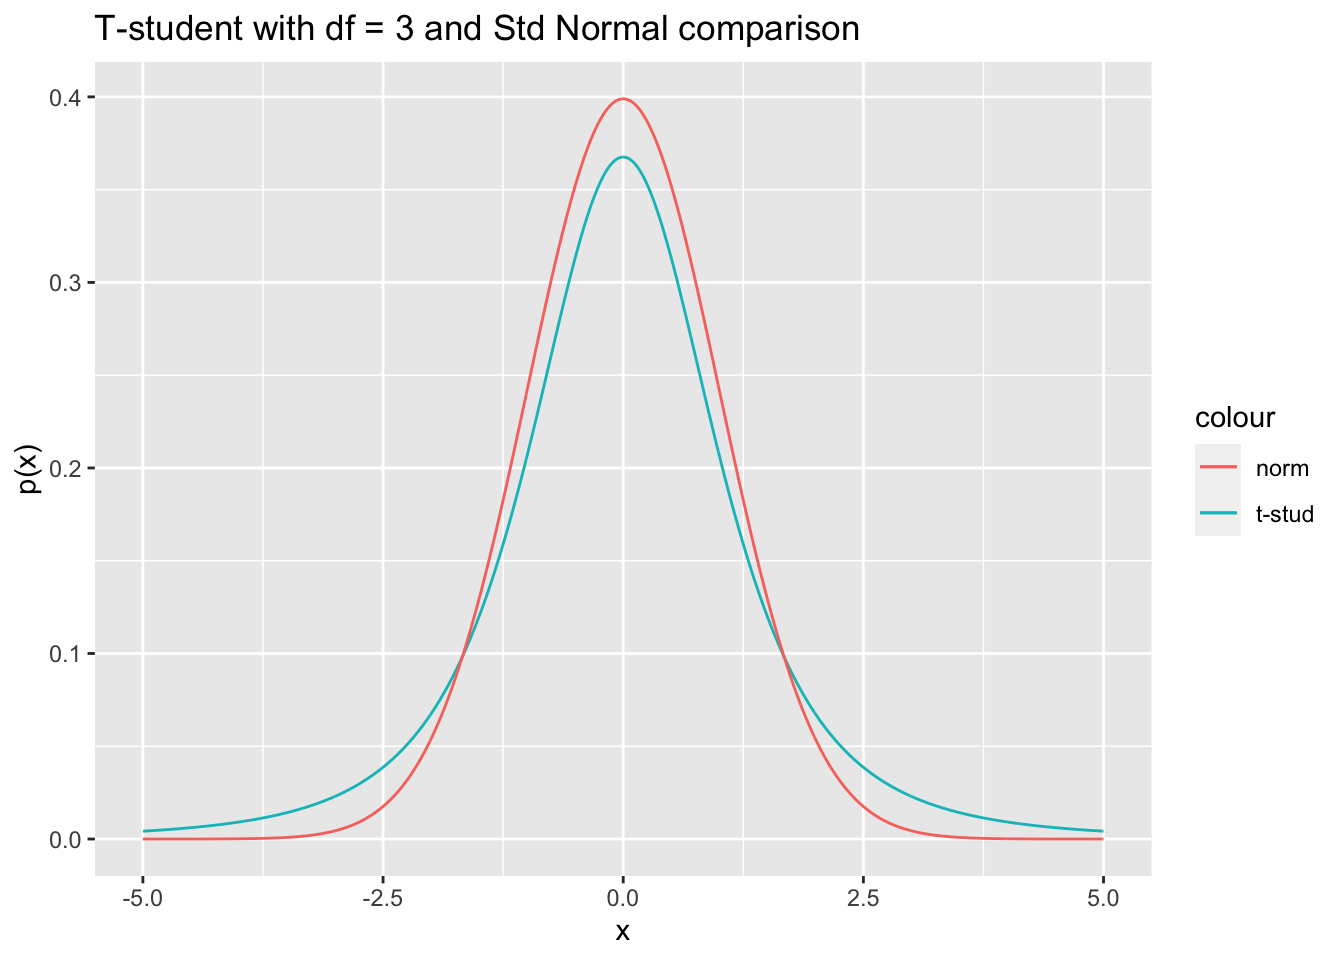
\includegraphics{smr_book_files/figure-latex/unnamed-chunk-61-1.pdf}
The plot indeed suggests that \(x_0 = 7\) is a good compromise,
but there is no rule in choosing such threshold, and in fact,
we might be more interested in a safer threshold in terms of lower
false alarm probability, or lower false non-alarm probability.

This decision process can be thought as two simple hypotheses test:
we consider the null hypothesis \(H_0: p = p_0\). Given our observation, i.e.~\(x\),
count of positive tests, realization of the \(X\) r.v.

\begin{itemize}
\tightlist
\item
  if \(x < x_0\) we have no reasons to reject \(H_0\)
\item
  if \(x \geq x_0\) we reject \(H_0\) and accept the alternative hypothesis
\end{itemize}

\subsection{The Binomial approximation}\label{the-binomial-approximation}

\textbf{Exercise}: The plot above shows that the Binomial distribution offers indeed
a good approximation of the Hypergeometric. However, as an exercise, we can
repeat the experiment changing the values of \(N\) and \(p\).

\begin{quote}
repeat the computations above tweaking the parameters and observe the
resulting plot. With which parameters do you observe a poor approximation of
the Hypergeometric with the Binomial distribution? Feel free to plot different
quantities, such as the density instead of the cumulative distribution
\end{quote}

\section{Confidence intervals}\label{confidence-intervals}

In case we have two samples \(\mathbf{X} = X_1, ..., X_m\) and
\(\mathbf{Y} = Y_1, ..., Y_n\) coming from two unknown Normal distributions, we
might want to test whether they come from distributions with same mean, or in
other words, whether they are both scattered around a common value. For example,
we could be interested in checking whether a set of jewelry items, which have
some variability in weight, has been produced in the same original
factory or if it is counterfeit.

After defining a confidence level \(1-\alpha\) and a variable that
we want to limit with some ``confidence'', we can compute the confidence interval
\((\Delta_l, \Delta_u)\). The confidence interval tells us where the
real value of the variable of interest can fall, with some
confidence given the evidence.
The higher is the confidence that we want to enforce, the larger the interval
will be, but remember that a wide confidence interval is often not useful.

\subsection{Example}\label{example-1}

Let's start with a simple example, where we have two normal samples,
of which we know nothing (not the mean, nor the variance):

\[
X_1, ..., X_m \stackrel{\text{i.i.d.}}{\sim} \mathcal N (\mu_x, \sigma_x^2)\,,\quad
Y_1, ..., Y_n \stackrel{\text{i.i.d.}}{\sim} \mathcal N (\mu_y, \sigma_y^2)
\]
The goal is to get a confidence interval for the variable \(\mu_x - \mu_y\),
therefore an interval in which we can expect the two means difference to be
with confidence \(1 - \alpha\).
Assuming that both \(n, m\) are sufficiently
large, the CI is computed as

\[
\bar{\mathbf{x}} - \bar{\mathbf{y}} \pm z_{\alpha/2}\sqrt{\frac{s_x^2}{m} +
\frac{s_y^2}{n}}\,.
\]

Let's simulate some data and use R to get the confidence interval, using as
paramters \(\mu_x = 10, \sigma_x^2 = 36\) and \(\mu_y = 10, \sigma_y^2 = 49\). We
draw \(m = 100\) and \(n = 120\) samples respectively.

\begin{Shaded}
\begin{Highlighting}[]
\CommentTok{\# set the parameters}
\NormalTok{m }\OtherTok{\textless{}{-}} \DecValTok{100}
\NormalTok{mu\_x }\OtherTok{\textless{}{-}} \DecValTok{10}
\NormalTok{sigma\_x }\OtherTok{\textless{}{-}} \DecValTok{6}
\NormalTok{n }\OtherTok{\textless{}{-}} \DecValTok{120}
\NormalTok{mu\_y }\OtherTok{\textless{}{-}} \DecValTok{10}
\NormalTok{sigma\_y }\OtherTok{\textless{}{-}} \DecValTok{7}

\CommentTok{\# use rnorm to draw independent and identically distributed samples}
\NormalTok{x }\OtherTok{\textless{}{-}} \FunctionTok{rnorm}\NormalTok{(m, mu\_x, sigma\_x)}
\NormalTok{y }\OtherTok{\textless{}{-}} \FunctionTok{rnorm}\NormalTok{(n, mu\_y, sigma\_y)}
\end{Highlighting}
\end{Shaded}

At this point we can define the confidence level and compute the CI.

\begin{Shaded}
\begin{Highlighting}[]
\NormalTok{alpha }\OtherTok{\textless{}{-}} \FloatTok{0.05} \CommentTok{\# typical value for alpha}

\CommentTok{\# define a custom function based on the formula above}
\NormalTok{confidence\_interval }\OtherTok{\textless{}{-}} \ControlFlowTok{function}\NormalTok{(x, y, alpha) \{}
  \CommentTok{\# note that mean() is the sample mean}
\NormalTok{  dev }\OtherTok{\textless{}{-}} \FunctionTok{mean}\NormalTok{(x) }\SpecialCharTok{{-}} \FunctionTok{mean}\NormalTok{(y)}
  \CommentTok{\# var() is the sample variance, not the actual variance}
\NormalTok{  delta }\OtherTok{\textless{}{-}} \FunctionTok{qnorm}\NormalTok{(}\DecValTok{1} \SpecialCharTok{{-}}\NormalTok{ alpha }\SpecialCharTok{/} \DecValTok{2}\NormalTok{) }\SpecialCharTok{*} \FunctionTok{sqrt}\NormalTok{(}\FunctionTok{var}\NormalTok{(x) }\SpecialCharTok{/}\NormalTok{ m }\SpecialCharTok{+} \FunctionTok{var}\NormalTok{(y) }\SpecialCharTok{/}\NormalTok{ n)}
  \FunctionTok{return}\NormalTok{(}\FunctionTok{c}\NormalTok{(dev }\SpecialCharTok{{-}}\NormalTok{ delta, dev }\SpecialCharTok{+}\NormalTok{ delta))}
\NormalTok{\}}

\FunctionTok{confidence\_interval}\NormalTok{(x, y, alpha)}
\end{Highlighting}
\end{Shaded}

\begin{verbatim}
## [1] -0.859210  2.540521
\end{verbatim}

We notice that the interval contains the value 0, and this
is due to the fact that both samples have same mean, therefore the
sample means will also be, with enough samples, very similar, thus with
zero (or close to zero) difference.

To wrap this up, under large sample assumptions and unknown variance,
we computed the confidence interval of a two-samples difference.
More in general, when we compare two samples \(\mathbf{x}, \mathbf{y}\)
there are multiple CIs that we might have to compute. We go through
them below.

\subsection{The four cases}\label{the-four-cases}

To better clarify, we can divide the confidence intervals over
two samples in four cases:

\begin{enumerate}
\def\labelenumi{\arabic{enumi}.}
\tightlist
\item
  we know the variances of the two samples, \(\sigma_x^2, \sigma_y^2\),
\item
  we don't know the variances, but the samples sizes are large enough,
\item
  we don't know the variances and we cannot assume large sample size, but we
  assume homoscedasticity (equal variances),
\item
  we don't know the variances, samples size is not large and homoscedasticity
  cannot be assumed.
\end{enumerate}

\subsubsection{Case 1}\label{case-1}

The variable of interest is, just like in any of the following cases,
\(\mu_x - \mu_y\), which we don't know.

What we do know, given normality of the samples and from some background theory,
is that

\[
\overline{\mathbf X} - \overline{\mathbf Y}\sim \mathcal N(\mu_x - 
\mu_y, \frac{\sigma_x^2}{m} + \frac{\sigma_y^2}{n})\,.
\]
Normalizing, we get

\[
\frac{\overline{\mathbf X} - \overline{\mathbf Y} - (\mu_x -
\mu_y)}{\sqrt{\frac{\sigma_x^2}{m} +
\frac{\sigma_y^2}{n}}}\sim \mathcal N(0, 1)\,,
\]
and thus, to get a confidence interval, we simply write the
\emph{coverage probability}

\[
P(- z_{\alpha/2} < \frac{\overline{\mathbf X} - \overline{\mathbf Y} - (\mu_x -
\mu_y)}{\sqrt{\frac{\sigma_x^2}{m} +
\frac{\sigma_y^2}{n}}} < z_{\alpha/2} ; \mu_x, \mu_y) \equiv 1 - \alpha
\]
and rearranging the terms we find the confidence interval for \(\mu_x - \mu_y\)
in case 1:

\[
\left( \overline{\mathbf X} - \overline{\mathbf Y} - z_{\alpha/2}
\sqrt{\frac{\sigma_x^2}{m} +
\frac{\sigma_y^2}{n}},  \overline{\mathbf X} - \overline{\mathbf Y} + z_{\alpha/2}
\sqrt{\frac{\sigma_x^2}{m} +
\frac{\sigma_y^2}{n}}\right)
\]

\subsubsection{Case 2}\label{case-2}

If \(m, n\) are ``large'', then the sample variance will asymptotically get
closer to the variance. In the previous example we assumed large sample
size, that's why we simply replaced \(\sigma\) with \(s\) in the above formula.

The interval
\[
\bar{\mathbf{x}} - \bar{\mathbf{y}} \pm z_{\alpha/2}\sqrt{\frac{s_x^2}{m} +
\frac{s_y^2}{n}}\,.
\]
is a confidence interval for \(\mu_x - \mu_y\) with \emph{approximately} level \(1-\alpha\).

\subsubsection{Case 3}\label{case-3}

In case we assume homoscedasticity, we leverage on the observation as much as we
can, therefore we compute a weighted average (\emph{pooled}) of the sample variances
and we use that estimator to approximate the common variance.

\[
s_p^2 = \frac{(m - 1) s_x^2 + (n - 1) s_y^2}{m + n - 2}\,.
\]
One can prove that the r.v
\(\frac{(m + n - 2) s_p^2}{\sigma^2} \sim \chi^2(m + n - 2)\) and from that
follows

\[
\frac{\overline{\mathbf X} - \overline{\mathbf Y} - (\mu_x -
\mu_y)}{\sqrt{s_p^2 \left( \frac{1}{m} +
\frac{1}{n}\right)}} \sim t(m + n - 2)\,,
\]
Where \(t(d)\) is a T-student distribution with \(d\) degrees of freedom and,
compared to a standard Normal distribution, has larger tails, which means that
the quantiles over small values such as \(\alpha\) will be higher wrt the std
normal.

\begin{Shaded}
\begin{Highlighting}[]
\NormalTok{x\_dt }\OtherTok{\textless{}{-}} \FunctionTok{seq}\NormalTok{(}\SpecialCharTok{{-}}\DecValTok{5}\NormalTok{, }\DecValTok{5}\NormalTok{, }\AttributeTok{by =} \FloatTok{0.01}\NormalTok{)}
\NormalTok{norm\_t\_df }\OtherTok{\textless{}{-}} \FunctionTok{tibble}\NormalTok{(}\AttributeTok{x =}\NormalTok{ x\_dt, }\AttributeTok{p\_dt =} \FunctionTok{dt}\NormalTok{(x, }\AttributeTok{df =} \DecValTok{3}\NormalTok{), }\AttributeTok{p\_nt =} \FunctionTok{dnorm}\NormalTok{(x))}

\NormalTok{norm\_t\_df }\SpecialCharTok{\%\textgreater{}\%}
  \FunctionTok{ggplot}\NormalTok{() }\SpecialCharTok{+}
  \FunctionTok{geom\_line}\NormalTok{(}\FunctionTok{aes}\NormalTok{(x, p\_dt, }\AttributeTok{color =} \StringTok{"t{-}stud"}\NormalTok{)) }\SpecialCharTok{+}
  \FunctionTok{geom\_line}\NormalTok{(}\FunctionTok{aes}\NormalTok{(x, p\_nt, }\AttributeTok{color =} \StringTok{"norm"}\NormalTok{)) }\SpecialCharTok{+}
  \FunctionTok{labs}\NormalTok{(}
    \AttributeTok{title =} \StringTok{"T{-}student with df = 3 and Std Normal comparison"}\NormalTok{,}
    \AttributeTok{x =} \StringTok{"x"}\NormalTok{, }\AttributeTok{y =} \StringTok{"p(x)"}
\NormalTok{  )}
\end{Highlighting}
\end{Shaded}

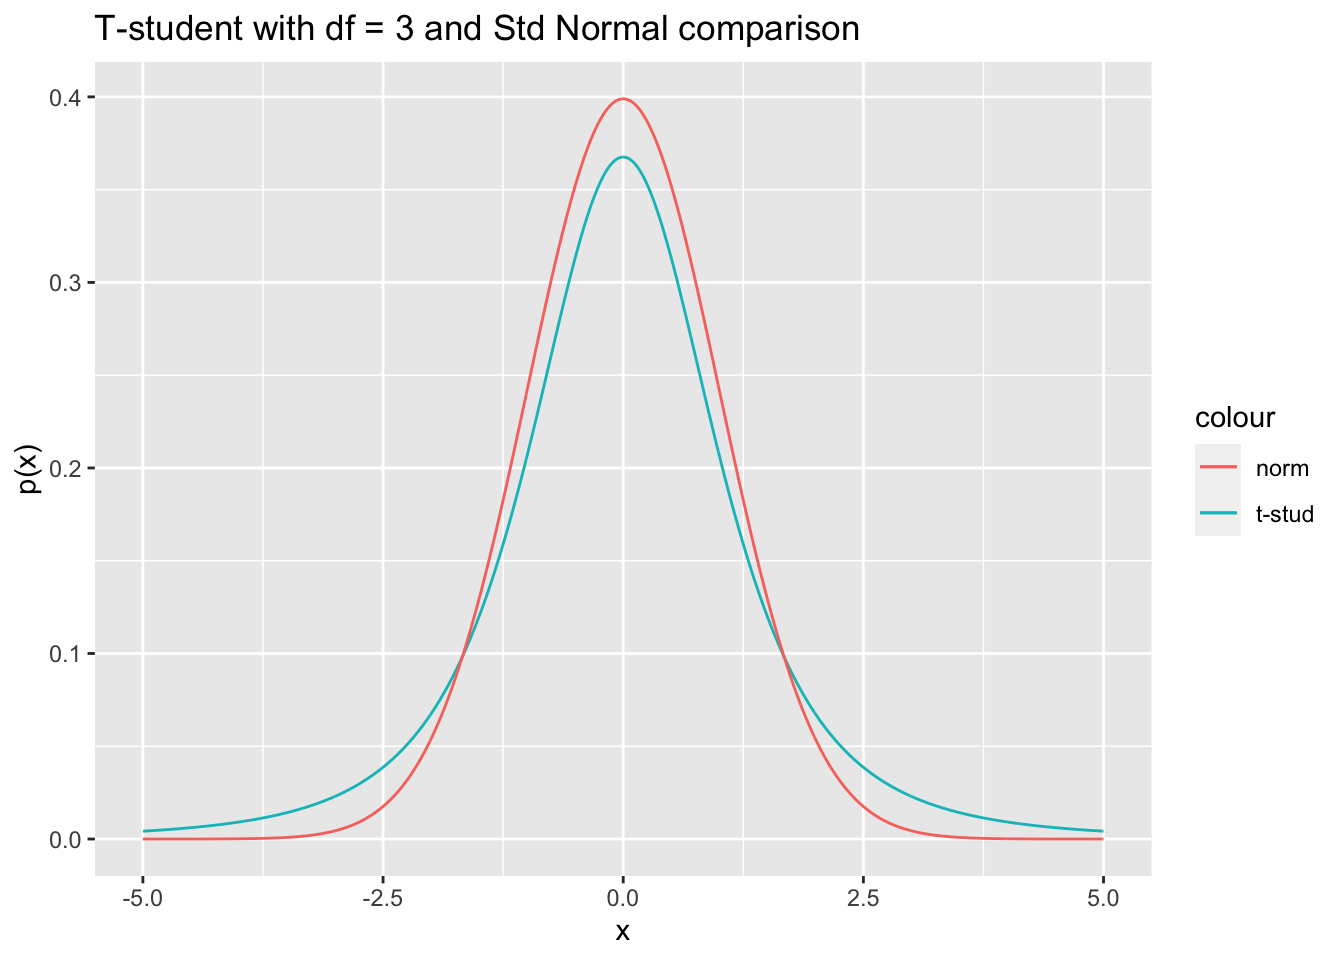
\includegraphics{smr_book_files/figure-latex/unnamed-chunk-64-1.pdf}

Following the same approach of the previous cases, the confidence interval
is found using the quantiles of the specific T-student distributions.

Before we computed the CI ``manually'', but luckily there exists a function which already implements this formula
(and not only this):

\begin{Shaded}
\begin{Highlighting}[]
\CommentTok{\# set var.equal = TRUE for pooled variance}
\NormalTok{test\_obj }\OtherTok{\textless{}{-}} \FunctionTok{t.test}\NormalTok{(x, y, }\AttributeTok{conf.level =} \DecValTok{1} \SpecialCharTok{{-}}\NormalTok{ alpha, }\AttributeTok{var.equal =} \ConstantTok{TRUE}\NormalTok{)}
\NormalTok{test\_obj }\CommentTok{\# outputs some information}
\end{Highlighting}
\end{Shaded}

\begin{verbatim}
## 
##  Two Sample t-test
## 
## data:  x and y
## t = 0.9646, df = 218, p-value = 0.3358
## alternative hypothesis: true difference in means is not equal to 0
## 95 percent confidence interval:
##  -0.8770073  2.5583183
## sample estimates:
## mean of x mean of y 
## 10.195089  9.354433
\end{verbatim}

\begin{Shaded}
\begin{Highlighting}[]
\NormalTok{test\_obj}\SpecialCharTok{$}\NormalTok{conf.int }\CommentTok{\# we\textquotesingle{}re interested in the confidence interval}
\end{Highlighting}
\end{Shaded}

\begin{verbatim}
## [1] -0.8770073  2.5583183
## attr(,"conf.level")
## [1] 0.95
\end{verbatim}

\subsubsection{Case 4}\label{case-4}

Otherwise, in case we cannot assume that the two samples have the same variance.
In R this specific confidence interval can be computed setting the \texttt{var.equal}
flag to false in \texttt{t.test()}.

\begin{Shaded}
\begin{Highlighting}[]
\CommentTok{\# or leaving it to default = F}
\FunctionTok{t.test}\NormalTok{(x, y, }\AttributeTok{var.equal =} \ConstantTok{FALSE}\NormalTok{) }\CommentTok{\# conf.level = 0.95 by default}
\end{Highlighting}
\end{Shaded}

\begin{verbatim}
## 
##  Welch Two Sample t-test
## 
## data:  x and y
## t = 0.96929, df = 214.36, p-value = 0.3335
## alternative hypothesis: true difference in means is not equal to 0
## 95 percent confidence interval:
##  -0.8688616  2.5501726
## sample estimates:
## mean of x mean of y 
## 10.195089  9.354433
\end{verbatim}

This is called the Welch-Satterthwaite approximation.

\section{P-value}\label{p-value}

In the context of hypothesis testing, the \emph{p-value} is the probability,
under the null hypothesis, that we obtain a test statistic at least as
contradictory to \(H_0\) as the statistic from the available sample.
In other words, it's a measure of the null hypothesis support in a 0 to 1 range.

\subsection{Example}\label{example-2}

In a fair French roulette, the red probability is 18/37.

\textbf{Questions:}

\begin{enumerate}
\def\labelenumi{\alph{enumi}.}
\tightlist
\item
  we observe 20 reds out of 30. Compute the p-value of the null hypothesis
  of the roulette being fair, with respect to the alternative hypothesis
  of the roulette being skewed towards the red,
\item
  in the same situation, compute the p-value of the null hypothesis
  of the roulette being fair wrt the alternative hypothesis of it not
  being fair,
\item
  repeat a. and b. with 200 reds out of 380 as outcome.
\end{enumerate}

\textbf{Answers:}

\begin{enumerate}
\def\labelenumi{\alph{enumi}.}
\tightlist
\item
  Given \(X = \#\text{reds}\), we can compute the following probability
  under the null hypothesis,
  noticing that \(X \sim \text{Binomial}(n, p)\) with \(n = 30\):
\end{enumerate}

\[
P(X \geq 20 | H_0) = \sum_{k = 20}^{30} {30 \choose k}
\left(\frac{18}{37}\right)^k\left(\frac{19}{37}\right)^{(30-k)}
\]
Note that we specify the condition \(\geq 20\) as the p-value stands for the
probability of observing an outcome \textbf{at least} as contradictory as the one
observed.

In R, we can compute it ``by hand'':

\begin{Shaded}
\begin{Highlighting}[]
\NormalTok{p0 }\OtherTok{\textless{}{-}} \DecValTok{18} \SpecialCharTok{/} \DecValTok{37}
\NormalTok{n }\OtherTok{\textless{}{-}} \DecValTok{30}
\CommentTok{\# P(X \textgreater{} 19) \textbackslash{}equiv P(X \textgreater{}= 20)}
\FunctionTok{pbinom}\NormalTok{(}\DecValTok{19}\NormalTok{, n, p0, }\AttributeTok{lower.tail =} \ConstantTok{FALSE}\NormalTok{) }\CommentTok{\# notice the lower.tail flag}
\end{Highlighting}
\end{Shaded}

\begin{verbatim}
## [1] 0.03598703
\end{verbatim}

or use the Binomial test function

\begin{Shaded}
\begin{Highlighting}[]
\CommentTok{\# check how it works}
\NormalTok{?binom.test}
\end{Highlighting}
\end{Shaded}

\begin{Shaded}
\begin{Highlighting}[]
\NormalTok{bin\_test }\OtherTok{\textless{}{-}} \FunctionTok{binom.test}\NormalTok{(}\DecValTok{20}\NormalTok{, n, p0, }\AttributeTok{alternative =} \StringTok{"greater"}\NormalTok{)}
\NormalTok{bin\_test}
\end{Highlighting}
\end{Shaded}

\begin{verbatim}
## 
##  Exact binomial test
## 
## data:  20 and n
## number of successes = 20, number of trials = 30, p-value = 0.03599
## alternative hypothesis: true probability of success is greater than 0.4864865
## 95 percent confidence interval:
##  0.5005613 1.0000000
## sample estimates:
## probability of success 
##              0.6666667
\end{verbatim}

\begin{Shaded}
\begin{Highlighting}[]
\NormalTok{bin\_test}\SpecialCharTok{$}\NormalTok{p.value}
\end{Highlighting}
\end{Shaded}

\begin{verbatim}
## [1] 0.03598703
\end{verbatim}

\begin{Shaded}
\begin{Highlighting}[]
\CommentTok{\# sketch of "greater" type p{-}value}
\NormalTok{sketch\_df }\OtherTok{\textless{}{-}} \FunctionTok{tibble}\NormalTok{(}\AttributeTok{x =} \DecValTok{0}\SpecialCharTok{:}\NormalTok{n, }\AttributeTok{px =} \FunctionTok{dbinom}\NormalTok{(x, n, p0))}
\NormalTok{sketch\_df }\SpecialCharTok{\%\textgreater{}\%}
  \FunctionTok{ggplot}\NormalTok{() }\SpecialCharTok{+}
  \FunctionTok{geom\_point}\NormalTok{(}\FunctionTok{aes}\NormalTok{(x, px)) }\SpecialCharTok{+}
  \FunctionTok{geom\_segment}\NormalTok{(}
    \AttributeTok{data =}\NormalTok{ . }\SpecialCharTok{\%\textgreater{}\%}\NormalTok{ dplyr}\SpecialCharTok{::}\FunctionTok{filter}\NormalTok{(x }\SpecialCharTok{\textgreater{}=} \DecValTok{20}\NormalTok{),}
    \FunctionTok{aes}\NormalTok{(}\AttributeTok{x =}\NormalTok{ x, }\AttributeTok{xend =}\NormalTok{ x, }\AttributeTok{y =} \DecValTok{0}\NormalTok{, }\AttributeTok{yend =}\NormalTok{ px), }\AttributeTok{color =} \DecValTok{2}
\NormalTok{  )}
\end{Highlighting}
\end{Shaded}

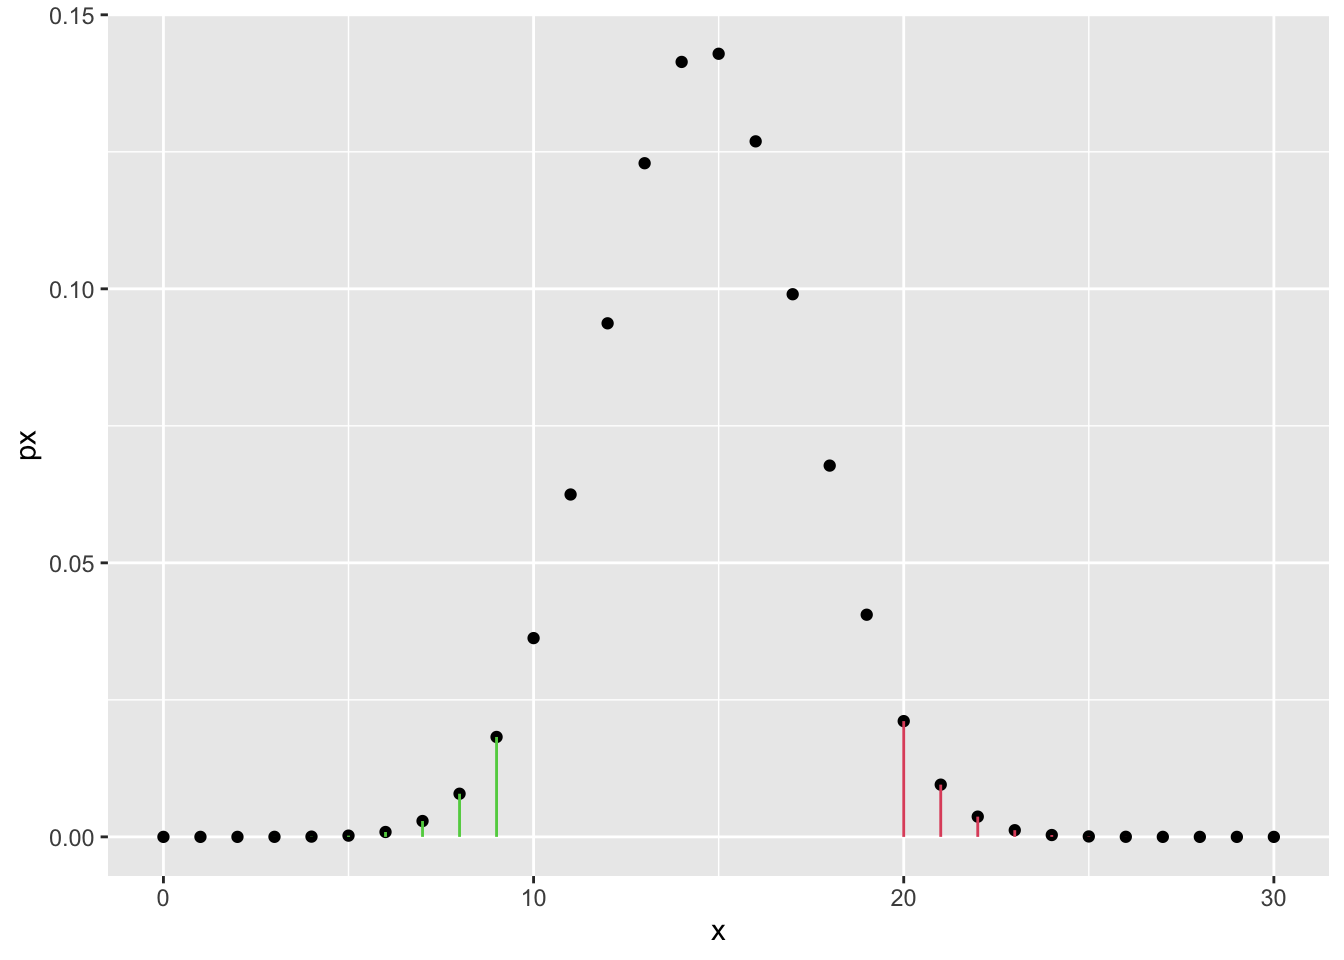
\includegraphics{smr_book_files/figure-latex/unnamed-chunk-70-1.pdf}

\begin{enumerate}
\def\labelenumi{\alph{enumi}.}
\setcounter{enumi}{1}
\tightlist
\item
  If the alternative hypothesis is just \(H_1: p \neq 18/37\) then the
  contradiction can happen both on the left and on the right side of the curve,
  i.e.~the roulette favors the red or the roulette favors the black \emph{in the
  same or more extreme way}.
  Therefore we have to sum the two probabilities:
\end{enumerate}

\[
P(X \geq 20 | H_0) + P(X < 10 | H_0)\,.
\]

\begin{quote}
Note: where does the 10 come from? Well, if we observe 20 reds out
of 30, at first we might think that the roulette prefers red instead
of black. One might argue that it does not prefer red, but rather
it is just not fair (no matter if it favors red or black). We then
have to consider \emph{all} cases that happen with a lower or equal
probability than the sample's. If the distribution is symmetric
(and in this case it almost is), we just consider \(X < 30 - 20\).
Check the probability \(P(X = 20)\) and find which values on the
left tail gives at most the same probability.
Those are the
values that must be considered in the two-sided test.
\end{quote}

We compute this quantity first using \texttt{pbinom} as before

\begin{Shaded}
\begin{Highlighting}[]
\FunctionTok{pbinom}\NormalTok{(}\DecValTok{19}\NormalTok{, n, p0, }\AttributeTok{lower.tail =} \ConstantTok{FALSE}\NormalTok{) }\SpecialCharTok{+} \FunctionTok{pbinom}\NormalTok{(}\DecValTok{9}\NormalTok{, n, p0)}
\end{Highlighting}
\end{Shaded}

\begin{verbatim}
## [1] 0.06614782
\end{verbatim}

and then using the test function

\begin{Shaded}
\begin{Highlighting}[]
\NormalTok{bin\_test\_2 }\OtherTok{\textless{}{-}} \FunctionTok{binom.test}\NormalTok{(}\DecValTok{20}\NormalTok{, n, p0, }\AttributeTok{alternative =} \StringTok{"two.sided"}\NormalTok{)}

\NormalTok{bin\_test\_2}
\end{Highlighting}
\end{Shaded}

\begin{verbatim}
## 
##  Exact binomial test
## 
## data:  20 and n
## number of successes = 20, number of trials = 30, p-value = 0.06615
## alternative hypothesis: true probability of success is not equal to 0.4864865
## 95 percent confidence interval:
##  0.4718800 0.8271258
## sample estimates:
## probability of success 
##              0.6666667
\end{verbatim}

\begin{Shaded}
\begin{Highlighting}[]
\NormalTok{bin\_test\_2}\SpecialCharTok{$}\NormalTok{p.value}
\end{Highlighting}
\end{Shaded}

\begin{verbatim}
## [1] 0.06614782
\end{verbatim}

\begin{Shaded}
\begin{Highlighting}[]
\CommentTok{\# sketch of bilateral type p{-}value}
\NormalTok{sketch\_df }\OtherTok{\textless{}{-}} \FunctionTok{tibble}\NormalTok{(}\AttributeTok{x =} \DecValTok{0}\SpecialCharTok{:}\NormalTok{n, }\AttributeTok{px =} \FunctionTok{dbinom}\NormalTok{(x, n, p0))}
\NormalTok{sketch\_df }\SpecialCharTok{\%\textgreater{}\%}
  \FunctionTok{ggplot}\NormalTok{() }\SpecialCharTok{+}
  \FunctionTok{geom\_point}\NormalTok{(}\FunctionTok{aes}\NormalTok{(x, px)) }\SpecialCharTok{+}
  \FunctionTok{geom\_segment}\NormalTok{(}
    \AttributeTok{data =}\NormalTok{ . }\SpecialCharTok{\%\textgreater{}\%}\NormalTok{ dplyr}\SpecialCharTok{::}\FunctionTok{filter}\NormalTok{(x }\SpecialCharTok{\textgreater{}=} \DecValTok{20}\NormalTok{),}
    \FunctionTok{aes}\NormalTok{(}\AttributeTok{x =}\NormalTok{ x, }\AttributeTok{xend =}\NormalTok{ x, }\AttributeTok{y =} \DecValTok{0}\NormalTok{, }\AttributeTok{yend =}\NormalTok{ px), }\AttributeTok{color =} \DecValTok{2}
\NormalTok{  ) }\SpecialCharTok{+}
  \FunctionTok{geom\_segment}\NormalTok{(}
    \AttributeTok{data =}\NormalTok{ . }\SpecialCharTok{\%\textgreater{}\%}\NormalTok{ dplyr}\SpecialCharTok{::}\FunctionTok{filter}\NormalTok{(x }\SpecialCharTok{\textless{}} \DecValTok{10}\NormalTok{),}
    \FunctionTok{aes}\NormalTok{(}\AttributeTok{x =}\NormalTok{ x, }\AttributeTok{xend =}\NormalTok{ x, }\AttributeTok{y =} \DecValTok{0}\NormalTok{, }\AttributeTok{yend =}\NormalTok{ px), }\AttributeTok{color =} \DecValTok{3}
\NormalTok{  )}
\end{Highlighting}
\end{Shaded}

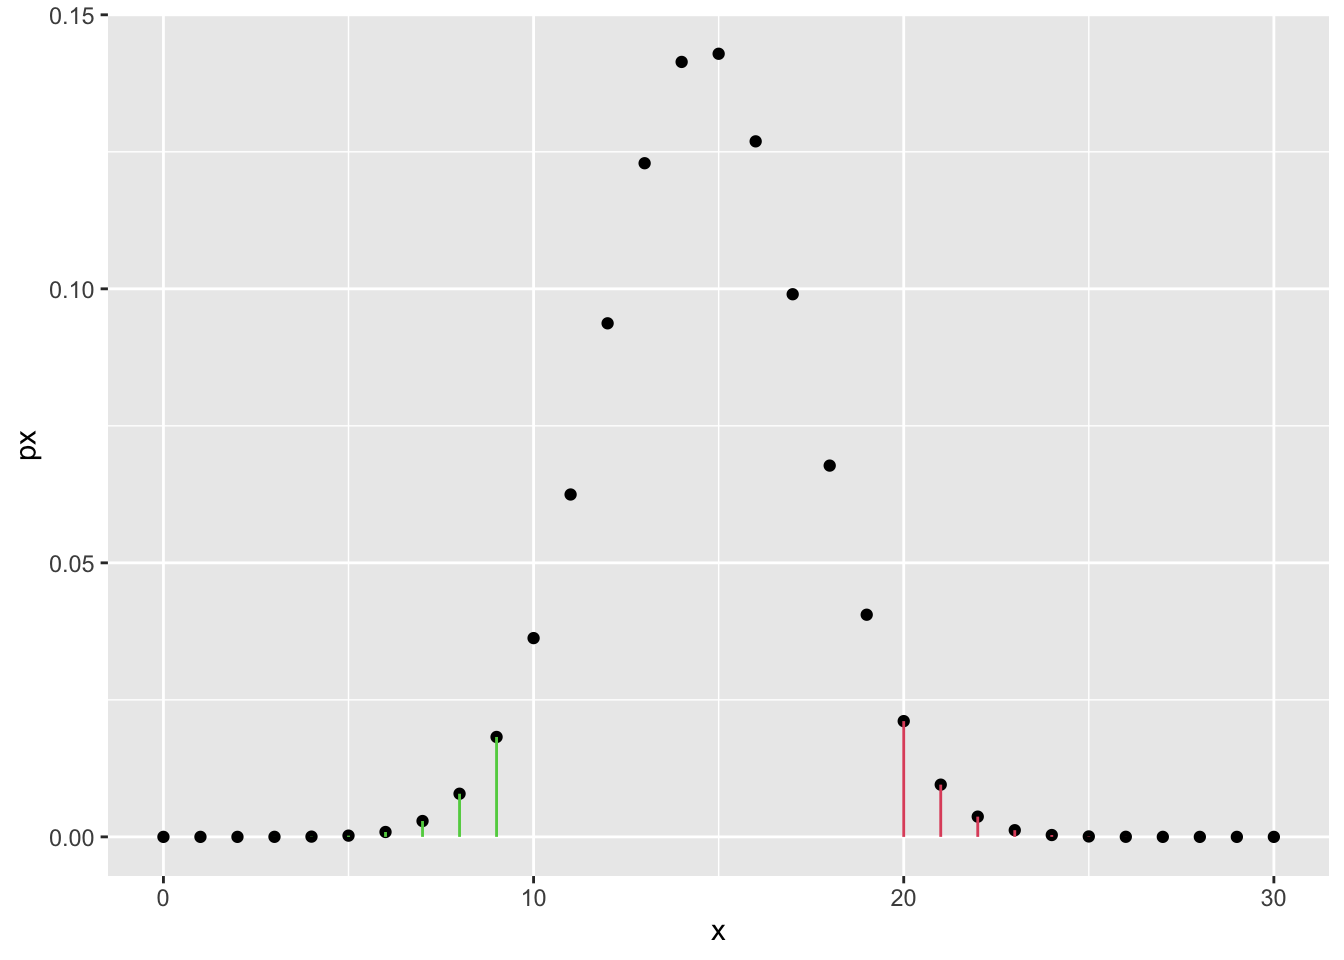
\includegraphics{smr_book_files/figure-latex/unnamed-chunk-73-1.pdf}

\begin{enumerate}
\def\labelenumi{\alph{enumi}.}
\setcounter{enumi}{2}
\tightlist
\item
  When \(n\) increases, and we can consider it large enough, we can
  use the normal approximation of the binomial (for the CLT), i.e.
\end{enumerate}

\[
Z = \frac{X - np}{\sqrt{np(1-p)}} \stackrel{n\rightarrow +\infty}{\approx} \mathcal
N(0,1)\,.
\]
Under the null hypothesis, in the unilateral case, we compute the p-value as

\[
P(Z \geq z | H_0) = 1 - \Phi(z)\,,
\]
where \(z\) is the realization of \(Z\) given that the realization of
\(X\) is \(x = 200\) (considered to be large enough for the approximation).

In R:

\begin{Shaded}
\begin{Highlighting}[]
\NormalTok{n }\OtherTok{\textless{}{-}} \DecValTok{380}
\NormalTok{x }\OtherTok{\textless{}{-}} \DecValTok{200}
\NormalTok{z }\OtherTok{\textless{}{-}}\NormalTok{ (x }\SpecialCharTok{{-}}\NormalTok{ n }\SpecialCharTok{*}\NormalTok{ p0) }\SpecialCharTok{/} \FunctionTok{sqrt}\NormalTok{(n }\SpecialCharTok{*}\NormalTok{ p0 }\SpecialCharTok{*}\NormalTok{ (}\DecValTok{1} \SpecialCharTok{{-}}\NormalTok{ p0))}
\FunctionTok{pnorm}\NormalTok{(z, }\AttributeTok{lower.tail =} \ConstantTok{FALSE}\NormalTok{)}
\end{Highlighting}
\end{Shaded}

\begin{verbatim}
## [1] 0.06016385
\end{verbatim}

or, using the R proportion test \texttt{prop.test}

\begin{Shaded}
\begin{Highlighting}[]
\NormalTok{?prop.test}
\end{Highlighting}
\end{Shaded}

\begin{Shaded}
\begin{Highlighting}[]
\FunctionTok{prop.test}\NormalTok{(x, n, }\AttributeTok{p =}\NormalTok{ p0, }\AttributeTok{alternative =} \StringTok{"greater"}\NormalTok{) }\CommentTok{\# uses continuity correction}
\end{Highlighting}
\end{Shaded}

\begin{verbatim}
## 
##  1-sample proportions test with continuity correction
## 
## data:  x out of n, null probability p0
## X-squared = 2.2562, df = 1, p-value = 0.06654
## alternative hypothesis: true p is greater than 0.4864865
## 95 percent confidence interval:
##  0.4828353 1.0000000
## sample estimates:
##         p 
## 0.5263158
\end{verbatim}

Notice that the result is not exactly the same. This is due to the fact
that we are approximating a discrete probability sum with an integral of
a Gaussian. To correct for this, it's enough to subtract (or add, depending
on the case) \texttt{.5} to the \(x\) value.

\begin{Shaded}
\begin{Highlighting}[]
\NormalTok{z\_corr }\OtherTok{\textless{}{-}}\NormalTok{ (x }\SpecialCharTok{{-}}\NormalTok{ .}\DecValTok{5} \SpecialCharTok{{-}}\NormalTok{ n }\SpecialCharTok{*}\NormalTok{ p0) }\SpecialCharTok{/} \FunctionTok{sqrt}\NormalTok{(n }\SpecialCharTok{*}\NormalTok{ p0 }\SpecialCharTok{*}\NormalTok{ (}\DecValTok{1} \SpecialCharTok{{-}}\NormalTok{ p0))}
\FunctionTok{pnorm}\NormalTok{(z\_corr, }\AttributeTok{lower.tail =} \ConstantTok{FALSE}\NormalTok{)}
\end{Highlighting}
\end{Shaded}

\begin{verbatim}
## [1] 0.06653798
\end{verbatim}

\begin{quote}
The bilateral case with Normal approximation is left to the reader as exercise
\end{quote}

\chapter{Normal sampling}\label{normal-sampling}

\section{Random and non-random normal samples}\label{random-and-non-random-normal-samples}

First we look at the simplest case: independent and identically distributed
Normal random variables.

\[
\mathbf{X} \sim \mathcal{N}\left(
\begin{pmatrix}
\mu \\ \vdots \\ \mu
\end{pmatrix}, 
\begin{pmatrix}
\sigma^2 & & & & \\
 & & & 0 & \\
 & & \ddots & &  \\
 & 0 & & & \\
 & & & & \sigma^2
\end{pmatrix}
\right)
\]

In order to simulate a sample of i.i.d. Normal r.v.,
we need to call the \texttt{rnorm} function, which uses R pseudo-random number generator.
Like every pseudo-RNG, it allows for specifying a seed, that
is useful for reproducibility purposes
(see \href{https://en.wikipedia.org/wiki/Pseudorandom_number_generator}{pseudo-RNG wiki} for
more details).

This is how you can simulate a
sample with \(n = 50\) i.i.d. Normal random variables in R.

\begin{Shaded}
\begin{Highlighting}[]
\FunctionTok{set.seed}\NormalTok{(}\DecValTok{42}\NormalTok{) }\CommentTok{\# for reproducibility}
\FunctionTok{library}\NormalTok{(ggplot2) }\CommentTok{\# plotting}
\FunctionTok{library}\NormalTok{(dplyr) }\CommentTok{\# dataframe manipulation}
\FunctionTok{library}\NormalTok{(tibble) }\CommentTok{\# tibble}

\NormalTok{n }\OtherTok{\textless{}{-}} \DecValTok{50}
\NormalTok{rnorm\_sample }\OtherTok{\textless{}{-}} \FunctionTok{rnorm}\NormalTok{(n) }\CommentTok{\# mu = 0, sigma = 1, for instance}

\NormalTok{iidplt }\OtherTok{\textless{}{-}}\NormalTok{ rnorm\_sample }\SpecialCharTok{\%\textgreater{}\%}
  \FunctionTok{enframe}\NormalTok{() }\SpecialCharTok{\%\textgreater{}\%} \CommentTok{\# creates tibble with name,value columns}
  \FunctionTok{ggplot}\NormalTok{() }\SpecialCharTok{+}
  \FunctionTok{geom\_point}\NormalTok{(}\FunctionTok{aes}\NormalTok{(}\AttributeTok{x =}\NormalTok{ name, }\AttributeTok{y =}\NormalTok{ value)) }\SpecialCharTok{+}
  \FunctionTok{labs}\NormalTok{(}\AttributeTok{title =} \StringTok{"Random sample"}\NormalTok{) }\SpecialCharTok{+} \CommentTok{\# add title and labels to the plot}
  \FunctionTok{xlab}\NormalTok{(}\StringTok{"i"}\NormalTok{) }\SpecialCharTok{+}
  \FunctionTok{ylab}\NormalTok{(}\StringTok{"x\_i"}\NormalTok{)}
\NormalTok{iidplt}
\end{Highlighting}
\end{Shaded}

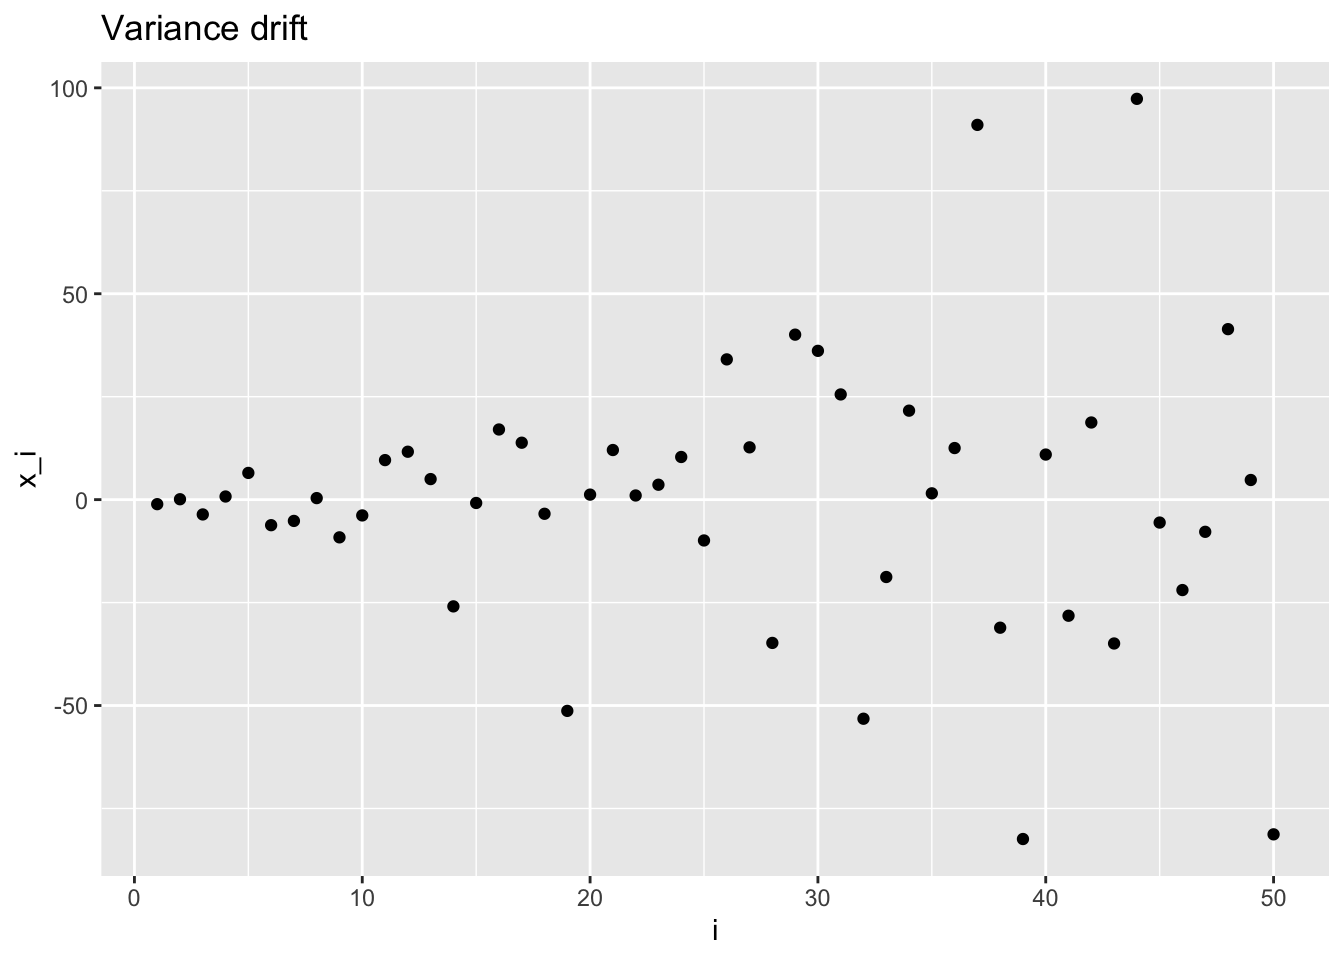
\includegraphics{smr_book_files/figure-latex/unnamed-chunk-79-1.pdf}

If the random variables are independent but distributed with different mean,
we can identify two notable cases: \textbf{mean shift} and \textbf{mean drift}.

In the first case, we write

\textbf{Mean shift}:
\[
\mathbf{X} \sim \mathcal{N}\left(
\begin{pmatrix}
\mu_0 \\ \vdots \\ \mu_0 \\ \mu_1 \\ \vdots \\ \mu_1
\end{pmatrix}, 
\begin{pmatrix}
\sigma^2 & & & & \\
 & & & 0 & \\
 & & \ddots & &  \\
 & 0 & & & \\
 & & & & \sigma^2
\end{pmatrix}
\right)\,,
\]

and in R we can simulate such sample as follows

\begin{Shaded}
\begin{Highlighting}[]
\CommentTok{\# (optional) creates a function to simplify other plots}
\NormalTok{plot\_sample }\OtherTok{\textless{}{-}} \ControlFlowTok{function}\NormalTok{(x, }\AttributeTok{title =} \ConstantTok{NULL}\NormalTok{, }\AttributeTok{xlab =} \ConstantTok{NULL}\NormalTok{, }\AttributeTok{ylab =} \ConstantTok{NULL}\NormalTok{) \{}
\NormalTok{  plt }\OtherTok{\textless{}{-}}\NormalTok{ x }\SpecialCharTok{\%\textgreater{}\%}
    \FunctionTok{enframe}\NormalTok{() }\SpecialCharTok{\%\textgreater{}\%}
    \FunctionTok{ggplot}\NormalTok{(}\FunctionTok{aes}\NormalTok{(}\AttributeTok{x =}\NormalTok{ name, }\AttributeTok{y =}\NormalTok{ value)) }\SpecialCharTok{+}
    \FunctionTok{geom\_point}\NormalTok{() }\SpecialCharTok{+}
    \FunctionTok{labs}\NormalTok{(}\AttributeTok{title =}\NormalTok{ title) }\SpecialCharTok{+}
    \FunctionTok{xlab}\NormalTok{(xlab) }\SpecialCharTok{+}
    \FunctionTok{ylab}\NormalTok{(ylab)}
  \FunctionTok{return}\NormalTok{(plt)}
\NormalTok{\}}

\CommentTok{\# first half with mean = 0, second half with mean = 3}
\CommentTok{\# simulate by concatenating two rnorm samples}
\NormalTok{ms\_sample }\OtherTok{\textless{}{-}} \FunctionTok{c}\NormalTok{(}\FunctionTok{rnorm}\NormalTok{(}\FunctionTok{floor}\NormalTok{(n }\SpecialCharTok{/} \DecValTok{2}\NormalTok{)), }\FunctionTok{rnorm}\NormalTok{(n }\SpecialCharTok{{-}} \FunctionTok{floor}\NormalTok{(n }\SpecialCharTok{/} \DecValTok{2}\NormalTok{), }\DecValTok{3}\NormalTok{))}
\CommentTok{\# or equivalently, by concatenating two mean vectors in one rnorm call}
\NormalTok{ms\_sample }\OtherTok{\textless{}{-}} \FunctionTok{rnorm}\NormalTok{(n, }\AttributeTok{mean =} \FunctionTok{c}\NormalTok{(}
  \FunctionTok{rep}\NormalTok{(}\DecValTok{0}\NormalTok{, }\FunctionTok{floor}\NormalTok{(n }\SpecialCharTok{/} \DecValTok{2}\NormalTok{)),}
  \FunctionTok{rep}\NormalTok{(}\DecValTok{3}\NormalTok{, n }\SpecialCharTok{{-}} \FunctionTok{floor}\NormalTok{(n }\SpecialCharTok{/} \DecValTok{2}\NormalTok{))}
\NormalTok{))}

\CommentTok{\# save the plot in a variable for later use}
\NormalTok{msplt }\OtherTok{\textless{}{-}} \FunctionTok{plot\_sample}\NormalTok{(ms\_sample, }\StringTok{"Mean{-}shift"}\NormalTok{, }\StringTok{"i"}\NormalTok{, }\StringTok{"x\_i"}\NormalTok{)}
\NormalTok{msplt}
\end{Highlighting}
\end{Shaded}

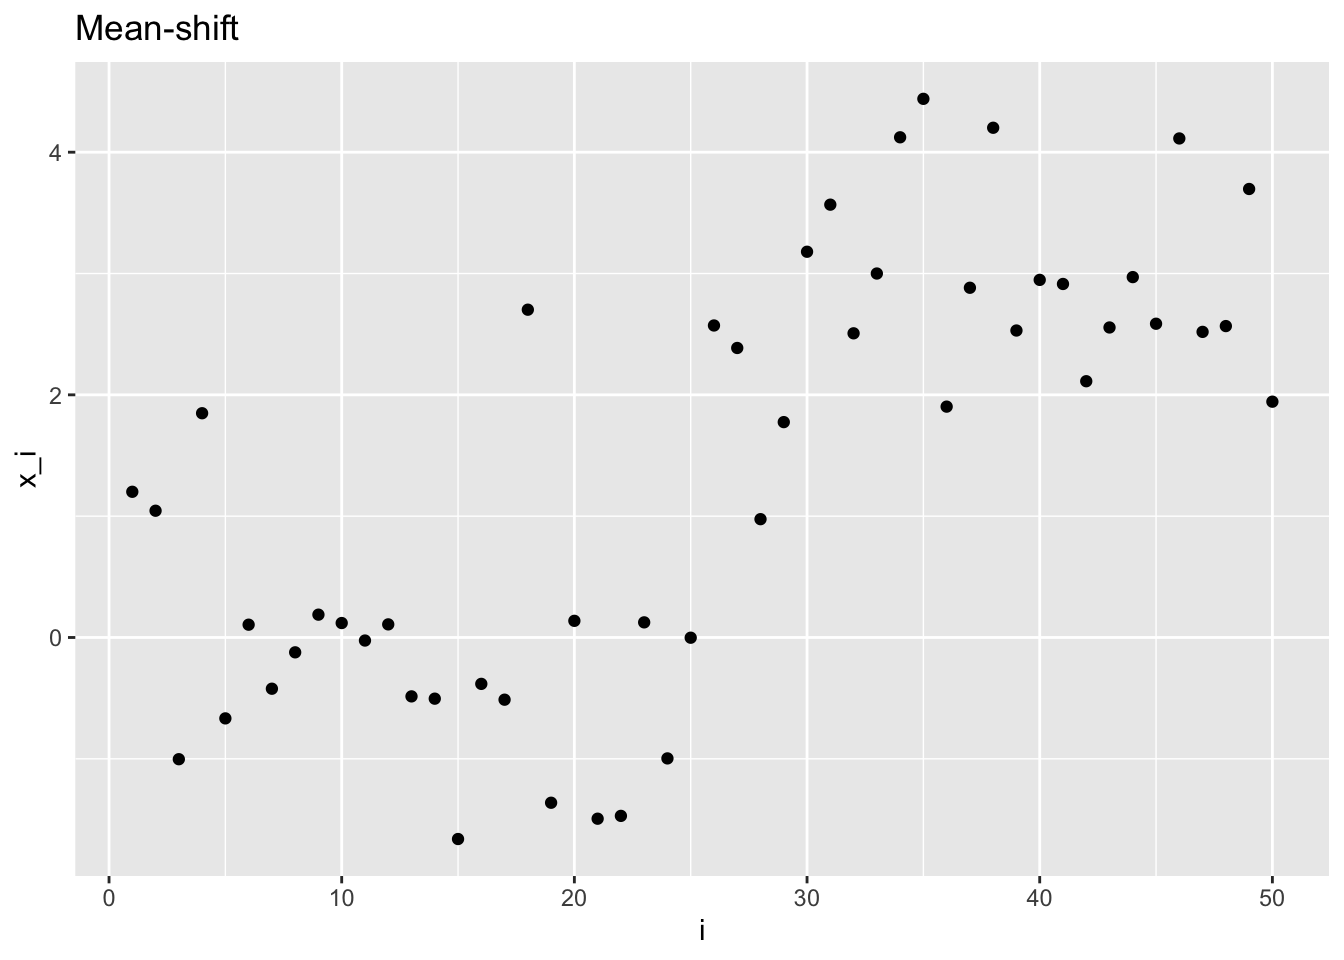
\includegraphics{smr_book_files/figure-latex/unnamed-chunk-80-1.pdf}

For the mean drift, the mean changes variable by variable

\textbf{Mean drift}:
\[
\mathbf{X} \sim \mathcal{N}\left(
\begin{pmatrix}
\mu_1 \\ \mu_2 \\ \vdots \\ \mu_n
\end{pmatrix}, 
\begin{pmatrix}
\sigma^2 & & & & \\
 & & & 0 & \\
 & & \ddots & &  \\
 & 0 & & & \\
 & & & & \sigma^2
\end{pmatrix}
\right)\,,
\]

Similarly, in R, we can simulate a mean drift with
mean going from \(0\) to \(n-1\) with unitary step.

\begin{Shaded}
\begin{Highlighting}[]
\CommentTok{\# mean is a range vector}
\NormalTok{md\_sample }\OtherTok{\textless{}{-}} \FunctionTok{rnorm}\NormalTok{(n, }\DecValTok{0}\SpecialCharTok{:}\NormalTok{(n }\SpecialCharTok{{-}} \DecValTok{1}\NormalTok{))}

\NormalTok{mdplt }\OtherTok{\textless{}{-}} \FunctionTok{plot\_sample}\NormalTok{(md\_sample, }\StringTok{"Mean drift"}\NormalTok{, }\StringTok{"i"}\NormalTok{, }\StringTok{"x\_i"}\NormalTok{)}
\NormalTok{mdplt}
\end{Highlighting}
\end{Shaded}

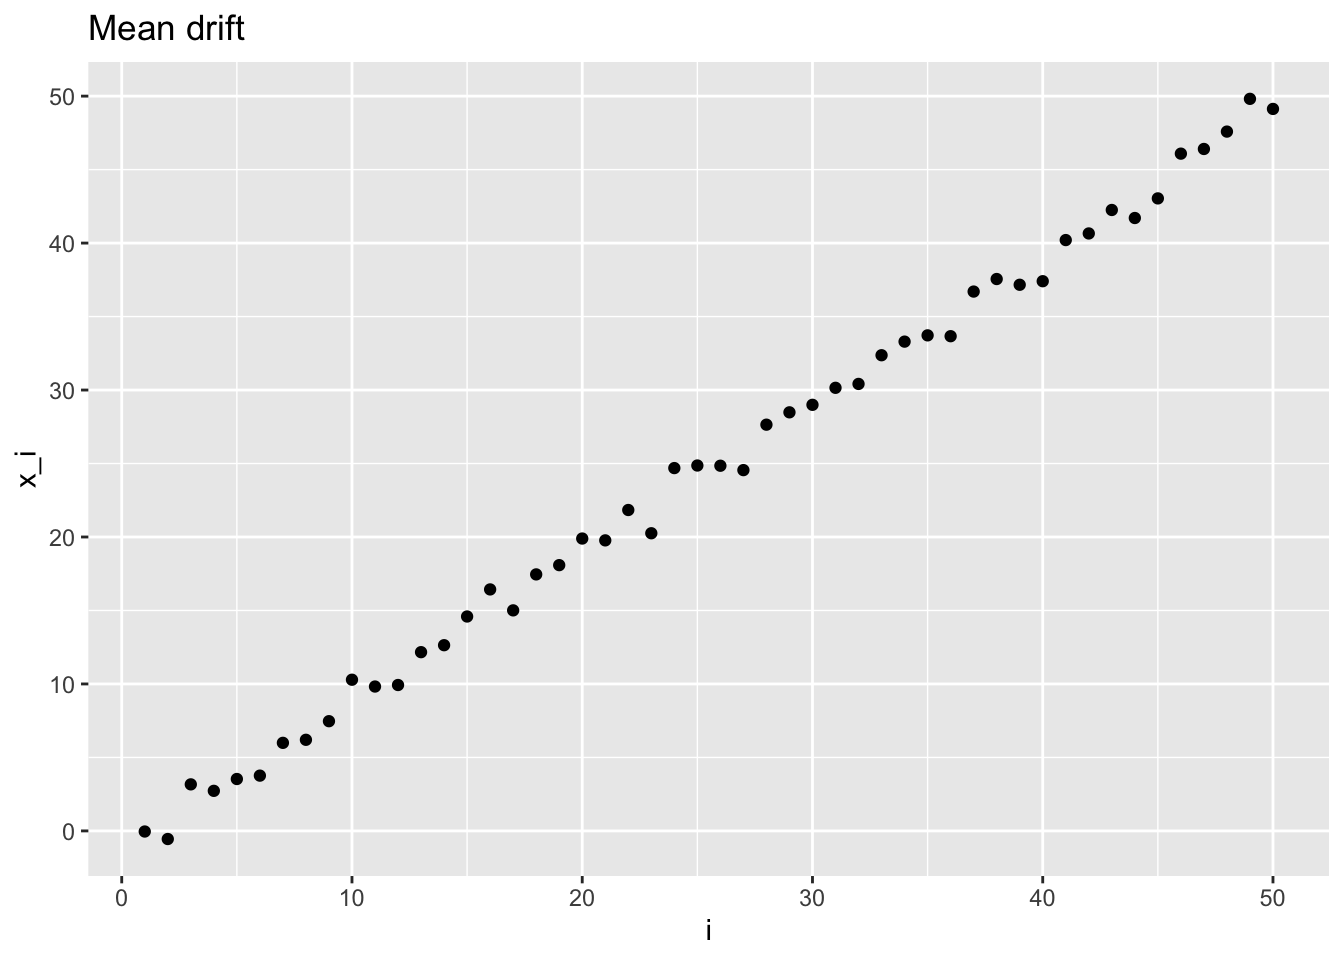
\includegraphics{smr_book_files/figure-latex/unnamed-chunk-81-1.pdf}

The same concept is applied also to random variables
drawn by a normal with changing variance.

\textbf{Variance shift}:
\[
\mathbf{X} \sim \mathcal{N}\left(
\begin{pmatrix}
\mu \\ \vdots \\ \mu
\end{pmatrix}, 
\begin{pmatrix}
\sigma_0^2 & & & & & \\
 & \ddots & & & 0 & \\
 & & \sigma_0^2 & & & \\
 & & & \sigma_1^2 & & \\
 & 0 & & & \ddots & \\
 & & & & & \sigma_1^2
\end{pmatrix}
\right)\,,
\]

in R:

\begin{Shaded}
\begin{Highlighting}[]
\NormalTok{vs\_sample }\OtherTok{\textless{}{-}} \FunctionTok{c}\NormalTok{(}
  \FunctionTok{rnorm}\NormalTok{(}\FunctionTok{floor}\NormalTok{(n }\SpecialCharTok{/} \DecValTok{2}\NormalTok{)), }\CommentTok{\# first half}
  \FunctionTok{rnorm}\NormalTok{(n }\SpecialCharTok{{-}} \FunctionTok{floor}\NormalTok{(n }\SpecialCharTok{/} \DecValTok{2}\NormalTok{), }\AttributeTok{sd =} \DecValTok{4}\NormalTok{)}
\NormalTok{) }\CommentTok{\# second half}

\NormalTok{vsplt }\OtherTok{\textless{}{-}} \FunctionTok{plot\_sample}\NormalTok{(vs\_sample, }\StringTok{"Variance shift"}\NormalTok{, }\StringTok{"i"}\NormalTok{, }\StringTok{"x\_i"}\NormalTok{)}
\NormalTok{vsplt}
\end{Highlighting}
\end{Shaded}

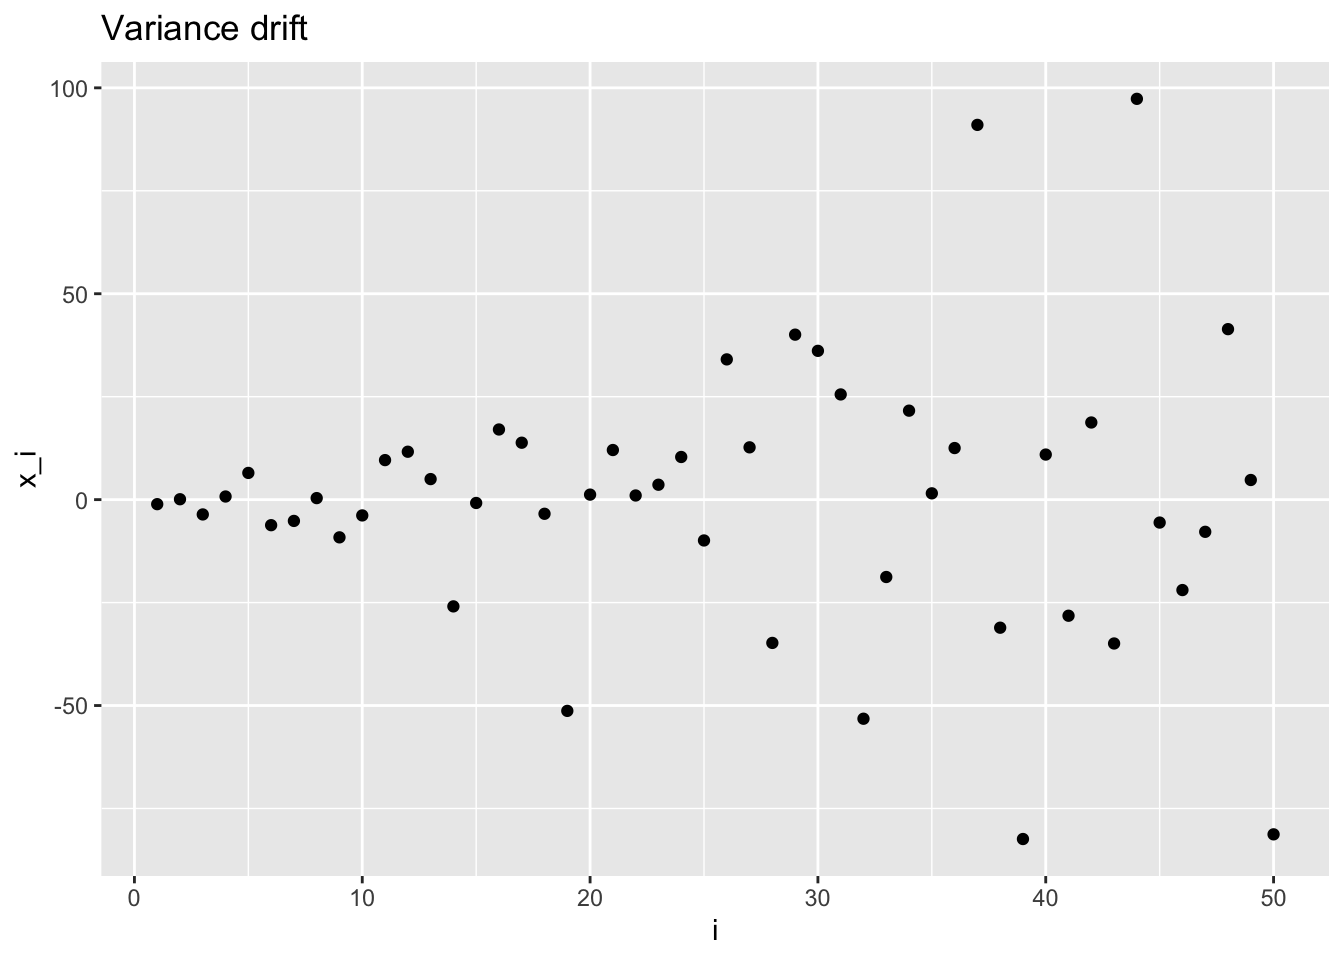
\includegraphics{smr_book_files/figure-latex/unnamed-chunk-82-1.pdf}

\textbf{Variance drift}

\[
\mathbf{X} \sim \mathcal{N}\left(
\begin{pmatrix}
\mu \\ \vdots \\ \mu
\end{pmatrix}, 
\begin{pmatrix}
\sigma_1^2 & & & & \\
 & & & 0 & \\
 & & \ddots & &  \\
 & 0 & & & \\
 & & & & \sigma_n^2
\end{pmatrix}
\right)\,,
\]

in R:

\begin{Shaded}
\begin{Highlighting}[]
\NormalTok{vd\_sample }\OtherTok{\textless{}{-}} \FunctionTok{rnorm}\NormalTok{(n, }\AttributeTok{sd =} \DecValTok{1}\SpecialCharTok{:}\NormalTok{n)}

\NormalTok{vdplt }\OtherTok{\textless{}{-}} \FunctionTok{plot\_sample}\NormalTok{(vd\_sample, }\StringTok{"Variance drift"}\NormalTok{, }\StringTok{"i"}\NormalTok{, }\StringTok{"x\_i"}\NormalTok{)}
\NormalTok{vdplt}
\end{Highlighting}
\end{Shaded}

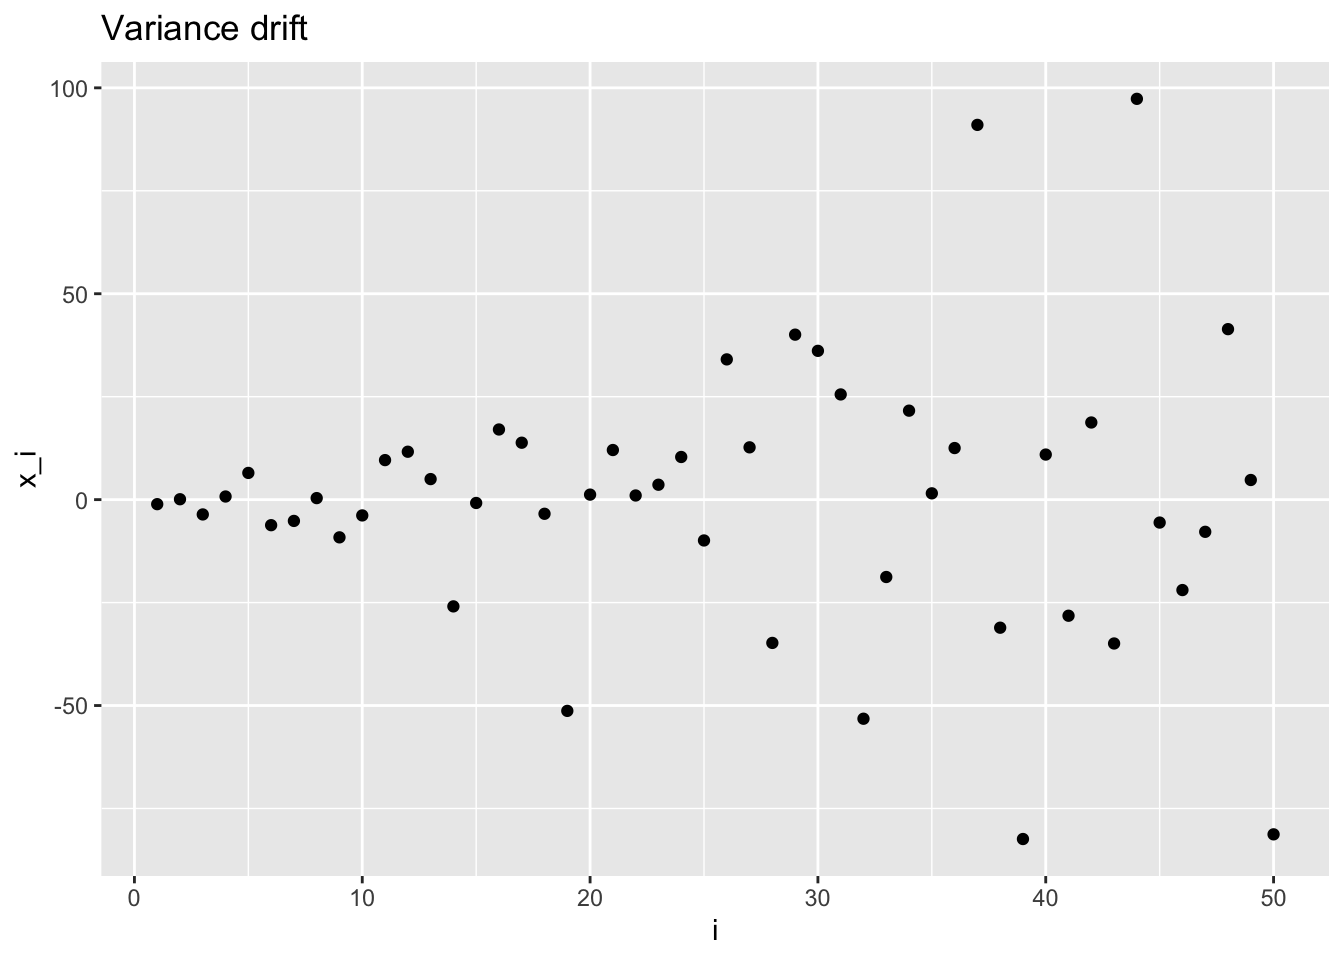
\includegraphics{smr_book_files/figure-latex/unnamed-chunk-83-1.pdf}

\subsection{Autocorrelated sample}\label{autocorrelated-sample}

Let \(\mathbf{Y} = Y_1, ..., Y_{n+1}\) an i.i.d. standard
Normal random sample (i.e.~\(Y_i \sim \mathcal{N}(0, 1)\)).

Then \(\mathbf{X} = X_1, ..., X_n\) such that \(X_i = Y_{i+1} - Y_i\) is
a Normal non-random sample with such distribution

\[
\mathbf{X} \sim \mathcal{N}\left(
\begin{pmatrix}
0 \\ \vdots \\ 0
\end{pmatrix}, 
\begin{pmatrix}
2 & -1 &  &  &  \\
-1 & 2 & & 0 & \\
 & & & & \\
 & \ddots & \ddots & \ddots &  \\
 & & & &  \\
 & 0 & & 2 & -1 \\
 & & & -1 & 2
\end{pmatrix}
\right)\,.
\]

The proof is left as exercise to the reader.

\begin{quote}
Hint: first compute \(E[X_i]\), then \(\text{Var}(X_i)\) and finally \(\text{Cov}(X_{i+1}, X_i)\)
\end{quote}

In R, we build this simulation by simulating \(\mathbf Y\) and deriving \(\mathbf X\)

\begin{Shaded}
\begin{Highlighting}[]
\NormalTok{y }\OtherTok{\textless{}{-}} \FunctionTok{rnorm}\NormalTok{(n)}
\CommentTok{\# index by removing first and last elements}
\NormalTok{auto\_sample }\OtherTok{\textless{}{-}}\NormalTok{ y[}\SpecialCharTok{{-}}\DecValTok{1}\NormalTok{] }\SpecialCharTok{{-}}\NormalTok{ y[}\SpecialCharTok{{-}}\NormalTok{n]}
\CommentTok{\# equivalent to}
\NormalTok{auto\_sample }\OtherTok{\textless{}{-}}\NormalTok{ y[}\DecValTok{2}\SpecialCharTok{:}\NormalTok{n] }\SpecialCharTok{{-}}\NormalTok{ y[}\DecValTok{1}\SpecialCharTok{:}\NormalTok{(n }\SpecialCharTok{{-}} \DecValTok{1}\NormalTok{)]}
\end{Highlighting}
\end{Shaded}

or, simpler

\begin{Shaded}
\begin{Highlighting}[]
\NormalTok{auto\_sample }\OtherTok{\textless{}{-}}\NormalTok{ y }\SpecialCharTok{\%\textgreater{}\%}
  \FunctionTok{diff}\NormalTok{()}
\NormalTok{auto\_sample}
\end{Highlighting}
\end{Shaded}

\begin{verbatim}
##  [1]  0.76486294 -0.72125125  0.69608123 -0.88154477  0.08858529  0.54025680
##  [7]  0.51057417 -2.23933913  1.21290797 -0.03747466 -0.68795847 -0.27543871
## [13]  0.40362741  1.21753967 -1.00313038 -0.36856515  0.94830413 -1.40013055
## [19]  2.28258801 -1.53046919  0.67372423 -0.13812248 -0.05124700  1.80962271
## [25] -2.63471000  1.97079841 -1.11389726 -0.86677899  0.76644216  0.81553534
## [31] -1.17229042 -0.34656350  0.92484634  0.83583274 -1.06205518 -1.31356822
## [37]  0.08035065  0.53828058  0.24128720  0.50568106  0.69192514 -1.10511511
## [43] -0.67926274  1.72098578 -0.33164903  0.88189010 -2.83982793  1.76979995
## [49]  1.26604281
\end{verbatim}

\begin{Shaded}
\begin{Highlighting}[]
\FunctionTok{plot\_sample}\NormalTok{(auto\_sample)}
\end{Highlighting}
\end{Shaded}

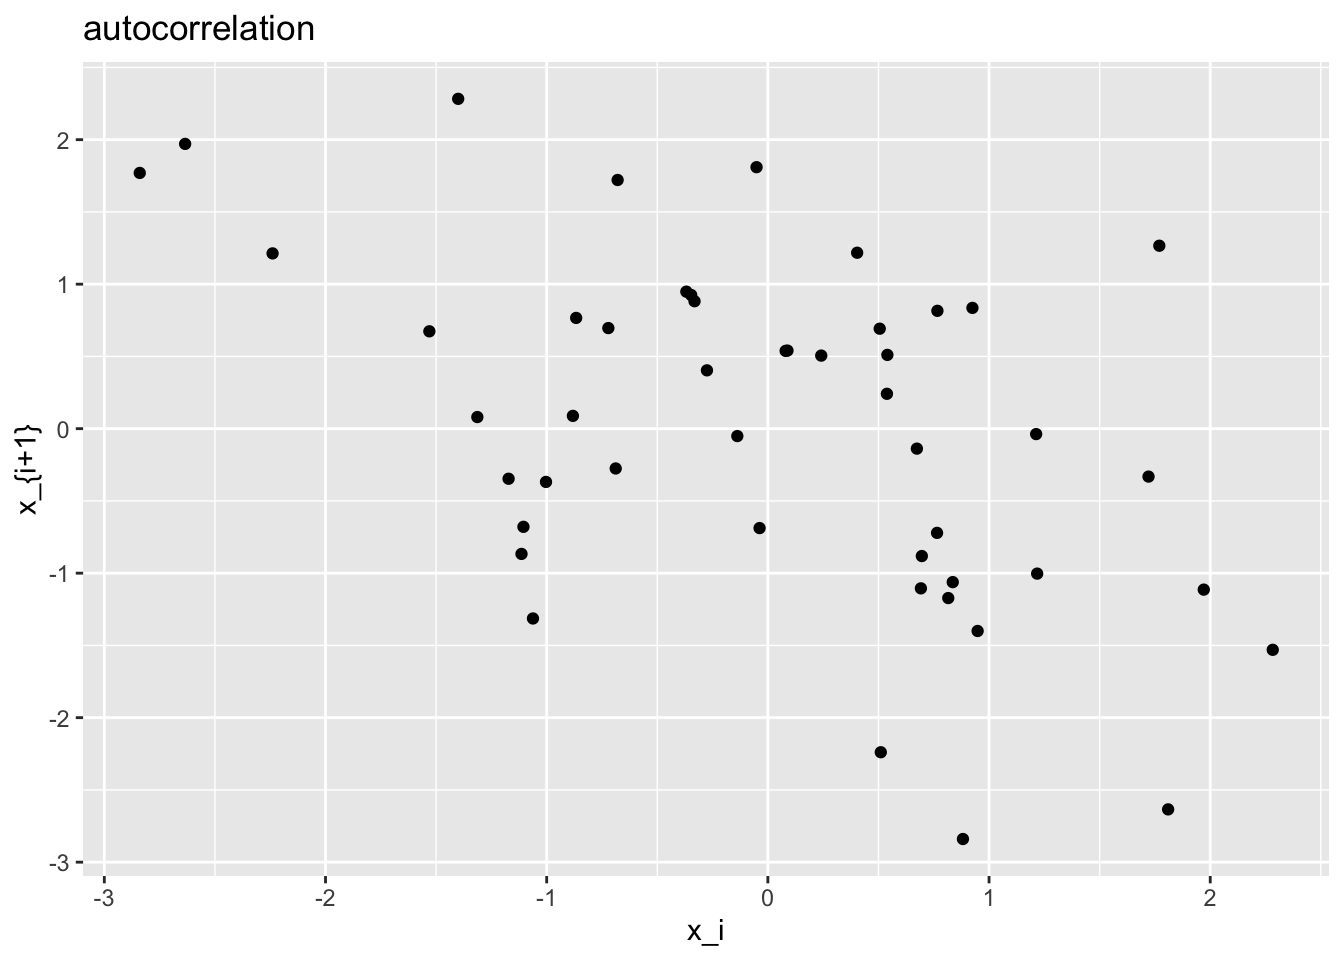
\includegraphics{smr_book_files/figure-latex/unnamed-chunk-85-1.pdf}

From this plot it is almost impossible to spot the correlation between variables.
It's more visible with a plot having \(X_i\) on one axis and \(X_{i+1}\) on the other.

\begin{Shaded}
\begin{Highlighting}[]
\NormalTok{autoplt }\OtherTok{\textless{}{-}}\NormalTok{ auto\_sample }\SpecialCharTok{\%\textgreater{}\%}
\NormalTok{  \{ }\CommentTok{\# group in curly brackets so that tibble is called}
    \CommentTok{\# without passing auto\_sample as first implicit argument}
    \FunctionTok{tibble}\NormalTok{(}\AttributeTok{x =}\NormalTok{ .[}\SpecialCharTok{{-}}\FunctionTok{length}\NormalTok{(.)], }\AttributeTok{y =}\NormalTok{ .[}\SpecialCharTok{{-}}\DecValTok{1}\NormalTok{]) }\CommentTok{\# dot as placeholder}
    \CommentTok{\# equivalent (but more efficient) to:}
    \CommentTok{\# tibble(x = auto\_sample[{-}length(auto\_sample)], y = auto\_sample[{-}1])}
\NormalTok{  \} }\SpecialCharTok{\%\textgreater{}\%}
  \FunctionTok{ggplot}\NormalTok{() }\SpecialCharTok{+}
  \FunctionTok{geom\_point}\NormalTok{(}\FunctionTok{aes}\NormalTok{(x, y)) }\SpecialCharTok{+}
  \FunctionTok{labs}\NormalTok{(}\AttributeTok{title =} \StringTok{"autocorrelation"}\NormalTok{) }\SpecialCharTok{+}
  \FunctionTok{xlab}\NormalTok{(}\StringTok{"x\_i"}\NormalTok{) }\SpecialCharTok{+}
  \FunctionTok{ylab}\NormalTok{(}\StringTok{"x\_\{i+1\}"}\NormalTok{)}
\NormalTok{autoplt}
\end{Highlighting}
\end{Shaded}

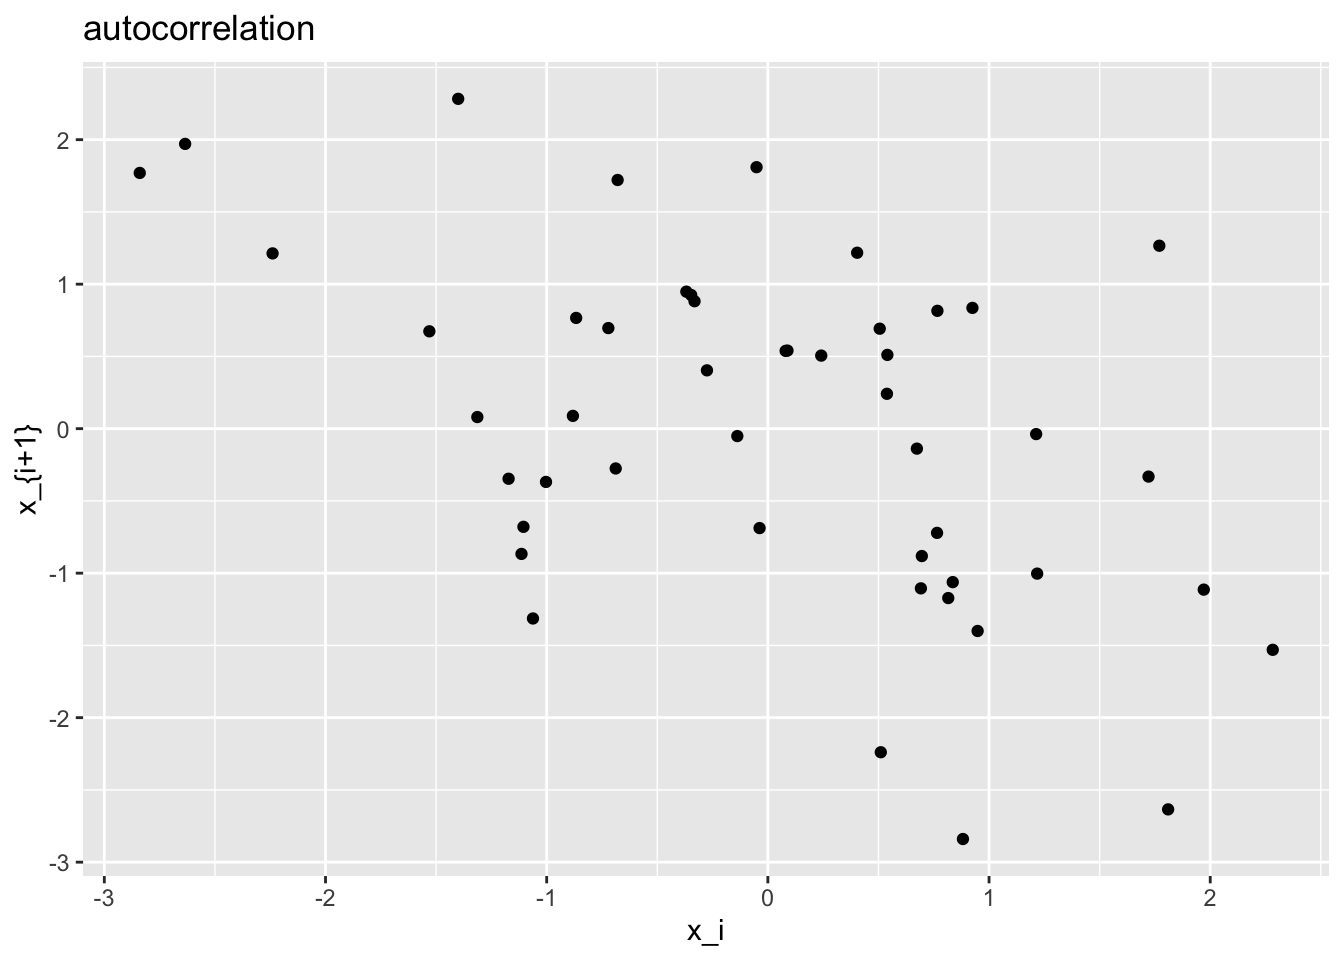
\includegraphics{smr_book_files/figure-latex/unnamed-chunk-86-1.pdf}

Maybe it's even more clear if the number of observations increases. Try with larger n.

\textbf{Questions}:

\begin{itemize}
\tightlist
\item
  how is \(X_i\) distributed?
\item
  what is the correlation between two subsequent samples i.e.~\(\rho(X_{i+1}, X_{i})\)
\end{itemize}

\textbf{Exercise}: build \texttt{Xpos} such that correlation is positive

We can compare these models by grouping all the plots in one
single picture.

\begin{Shaded}
\begin{Highlighting}[]
\CommentTok{\# install.packages("ggpubr")}
\FunctionTok{library}\NormalTok{(ggpubr)}
\FunctionTok{ggarrange}\NormalTok{(iidplt, msplt, mdplt, vsplt, vdplt, autoplt,}
  \AttributeTok{nrow =} \DecValTok{3}\NormalTok{, }\AttributeTok{ncol =} \DecValTok{2}
\NormalTok{)}
\end{Highlighting}
\end{Shaded}

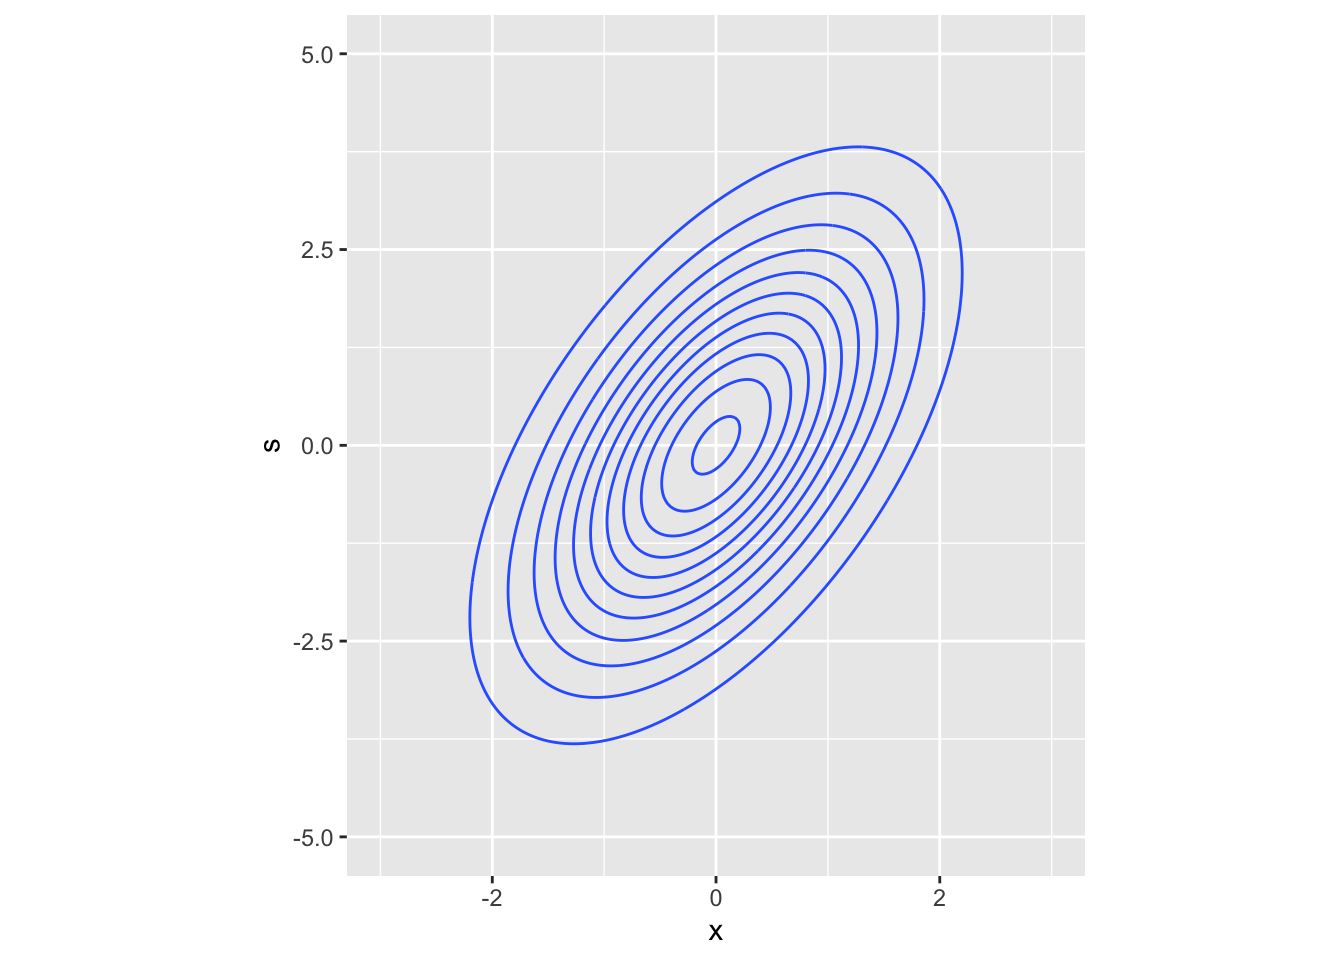
\includegraphics{smr_book_files/figure-latex/unnamed-chunk-87-1.pdf}

\section{Exchangeable normal random variables}\label{exchangeable-normal-random-variables}

Let \(\mathbf{X} = (X_1, ..., X_n)\) be a random vector whose elements
follow the conditional distribution
\[
X_i | \mu \sim \mathcal{N}(\mu, \sigma^2)
\]
with \(\mu\) being another normally distributed r.v.
\[
\mu \sim \mathcal{N}(\mu_0, \sigma_0^2)\,.
\]

\(X_i\) are conditionally independent given \(\mu\), and also,
their joint distribution is equal for any permutation
of the random vector elements (exchangeable).
But if we don't know \(\mu\), what is the distribution of
\(X_i\) (marginal distribution)?

It's

\[
\mathbf{X} \sim \mathcal{N}\left(\begin{pmatrix}
\mu_0 \\ \vdots \\ \mu_0
\end{pmatrix}, 
\begin{pmatrix}
\sigma^2 + \sigma_0^2 & & & & \\
 & \ddots & & \sigma_0^2 & \\
 & & \ddots & &  \\
 & \sigma_0^2 & & \ddots & \\
 & & & & \sigma^2 + \sigma_0^2
\end{pmatrix}
\right)
\]

\textbf{Exercise}: prove it (i.e.~find expected value, variance and covariance).

\begin{quote}
Hint: \(E[X_i] = E_{f\sim \mu}[E_{f\sim X_i | \mu}[X_i | \mu]]\)
\end{quote}

In R, we simply simulate a realization of the mean r.v., then
use that value to simulate the \(\mathbf X\) Normal sample given \(\mu\).

\begin{Shaded}
\begin{Highlighting}[]
\NormalTok{mu }\OtherTok{\textless{}{-}} \FunctionTok{rnorm}\NormalTok{(}\DecValTok{1}\NormalTok{)}
\NormalTok{x }\OtherTok{\textless{}{-}} \FunctionTok{rnorm}\NormalTok{(n, mu)}
\end{Highlighting}
\end{Shaded}

\section{Multivariate Normal random samples}\label{multivariate-normal-random-samples}

Multivariate normal distribution functions are provided by the \texttt{mvtnorm} library.

Take this as an example:

\[
\begin{pmatrix} X \\ S \end{pmatrix} \sim
\mathcal{N} \left(
\begin{pmatrix}
0 \\ 0
\end{pmatrix},
\begin{pmatrix}
1 & 1 \\ 1 & 3
\end{pmatrix}
\right)
\]

\begin{Shaded}
\begin{Highlighting}[]
\CommentTok{\# install.packages("mvtnorm")}
\FunctionTok{library}\NormalTok{(mvtnorm)}

\CommentTok{\# simulate n bivariate normal r.v.}
\NormalTok{m }\OtherTok{\textless{}{-}} \FunctionTok{rep}\NormalTok{(}\DecValTok{0}\NormalTok{, }\DecValTok{2}\NormalTok{) }\CommentTok{\# mean vector}
\NormalTok{vcov\_mat }\OtherTok{\textless{}{-}} \FunctionTok{matrix}\NormalTok{(}\FunctionTok{c}\NormalTok{(}\DecValTok{1}\NormalTok{, }\DecValTok{1}\NormalTok{, }\DecValTok{1}\NormalTok{, }\DecValTok{3}\NormalTok{), }\AttributeTok{nrow =} \DecValTok{2}\NormalTok{) }\CommentTok{\# Sigma}

\CommentTok{\# specify mean vector and var{-}cov matrix}
\NormalTok{bvt\_samples }\OtherTok{\textless{}{-}}\NormalTok{ mvtnorm}\SpecialCharTok{::}\FunctionTok{rmvnorm}\NormalTok{(n, m, vcov\_mat)}
\FunctionTok{head}\NormalTok{(bvt\_samples, }\DecValTok{10}\NormalTok{) }\CommentTok{\# print only the first 10 elements}
\end{Highlighting}
\end{Shaded}

\begin{verbatim}
##              [,1]       [,2]
##  [1,] -0.78186845 -0.2389248
##  [2,] -0.17599524 -0.9582082
##  [3,] -0.92364519 -0.3863103
##  [4,]  1.17077708  2.7456040
##  [5,] -2.03263913 -1.9171945
##  [6,] -0.92418665 -2.9286612
##  [7,] -0.99088212 -1.6003554
##  [8,] -1.50519809 -3.9739964
##  [9,] -0.04465341 -0.9858018
## [10,]  1.70934985  1.9264325
\end{verbatim}

Let's plot this sample

\begin{Shaded}
\begin{Highlighting}[]
\NormalTok{bvt\_samples\_df }\OtherTok{\textless{}{-}} \FunctionTok{tibble}\NormalTok{(}\AttributeTok{x =}\NormalTok{ bvt\_samples[, }\DecValTok{1}\NormalTok{], }\AttributeTok{s =}\NormalTok{ bvt\_samples[, }\DecValTok{2}\NormalTok{])}
\NormalTok{bvt\_scatter }\OtherTok{\textless{}{-}}\NormalTok{ bvt\_samples\_df }\SpecialCharTok{\%\textgreater{}\%}
  \FunctionTok{ggplot}\NormalTok{() }\SpecialCharTok{+}
  \FunctionTok{geom\_point}\NormalTok{(}\FunctionTok{aes}\NormalTok{(x, s)) }\SpecialCharTok{+}
  \FunctionTok{coord\_fixed}\NormalTok{(}\AttributeTok{xlim =} \FunctionTok{c}\NormalTok{(}\SpecialCharTok{{-}}\DecValTok{3}\NormalTok{, }\DecValTok{3}\NormalTok{), }\AttributeTok{ylim =} \FunctionTok{c}\NormalTok{(}\SpecialCharTok{{-}}\DecValTok{5}\NormalTok{, }\DecValTok{5}\NormalTok{), }\AttributeTok{ratio =} \SpecialCharTok{{-}}\NormalTok{.}\DecValTok{7}\NormalTok{)}

\NormalTok{bvt\_scatter}
\end{Highlighting}
\end{Shaded}

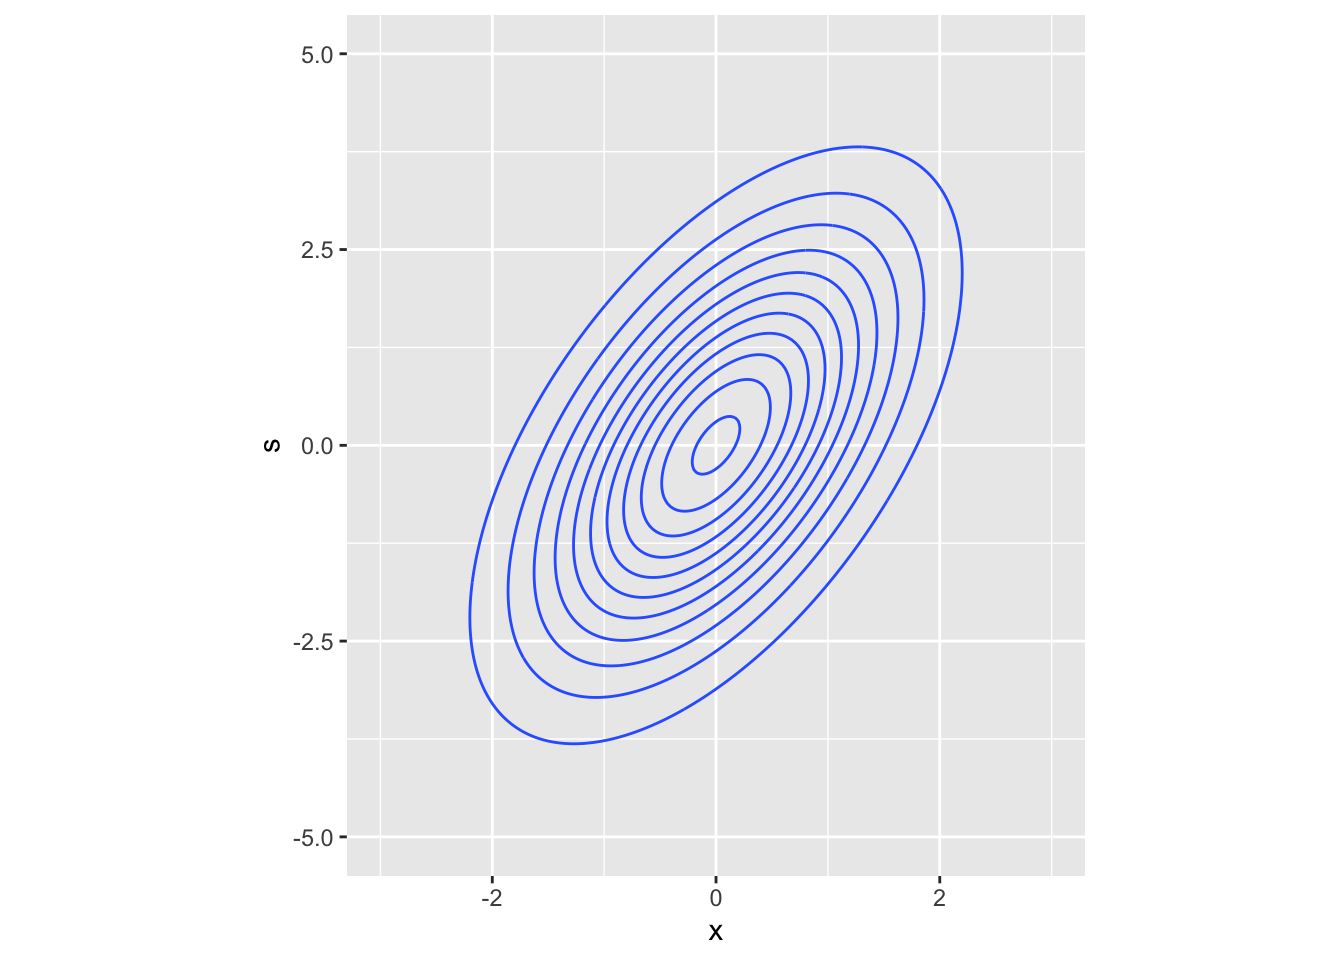
\includegraphics{smr_book_files/figure-latex/unnamed-chunk-90-1.pdf}

\begin{Shaded}
\begin{Highlighting}[]
\CommentTok{\# plot the true distribution}
\CommentTok{\# generate a grid (many points with fixed space between them)}
\NormalTok{bvt\_grid }\OtherTok{\textless{}{-}} \FunctionTok{expand.grid}\NormalTok{(}
  \AttributeTok{x =} \FunctionTok{seq}\NormalTok{(}\SpecialCharTok{{-}}\DecValTok{3}\NormalTok{, }\DecValTok{3}\NormalTok{, }\AttributeTok{length.out =} \DecValTok{200}\NormalTok{), }\CommentTok{\# seq builds a sequence vector starting from}
  \CommentTok{\# 3 until 3 with step such that the number of elements in the vector is 200}
  \AttributeTok{s =} \FunctionTok{seq}\NormalTok{(}\SpecialCharTok{{-}}\DecValTok{4}\NormalTok{, }\DecValTok{4}\NormalTok{, }\AttributeTok{length.out =} \DecValTok{200}\NormalTok{)}
\NormalTok{)}

\CommentTok{\# compute the density at each coordinate of the grid}
\NormalTok{probs }\OtherTok{\textless{}{-}} \FunctionTok{dmvnorm}\NormalTok{(bvt\_grid, m, vcov\_mat)}
\NormalTok{bvt\_grid }\SpecialCharTok{\%\textgreater{}\%}
  \FunctionTok{mutate}\NormalTok{(}\AttributeTok{prob =}\NormalTok{ probs) }\SpecialCharTok{\%\textgreater{}\%} \CommentTok{\# add a column (?dplyr::mutate)}
  \FunctionTok{ggplot}\NormalTok{() }\SpecialCharTok{+}
  \FunctionTok{geom\_contour}\NormalTok{(}\FunctionTok{aes}\NormalTok{(x, s, }\AttributeTok{z =}\NormalTok{ prob)) }\SpecialCharTok{+} \CommentTok{\# or geom\_contour\_filled}
  \FunctionTok{coord\_fixed}\NormalTok{(}\AttributeTok{xlim =} \FunctionTok{c}\NormalTok{(}\SpecialCharTok{{-}}\DecValTok{3}\NormalTok{, }\DecValTok{3}\NormalTok{), }\AttributeTok{ylim =} \FunctionTok{c}\NormalTok{(}\SpecialCharTok{{-}}\DecValTok{5}\NormalTok{, }\DecValTok{5}\NormalTok{), }\AttributeTok{ratio =} \SpecialCharTok{{-}}\NormalTok{.}\DecValTok{7}\NormalTok{)}
\end{Highlighting}
\end{Shaded}

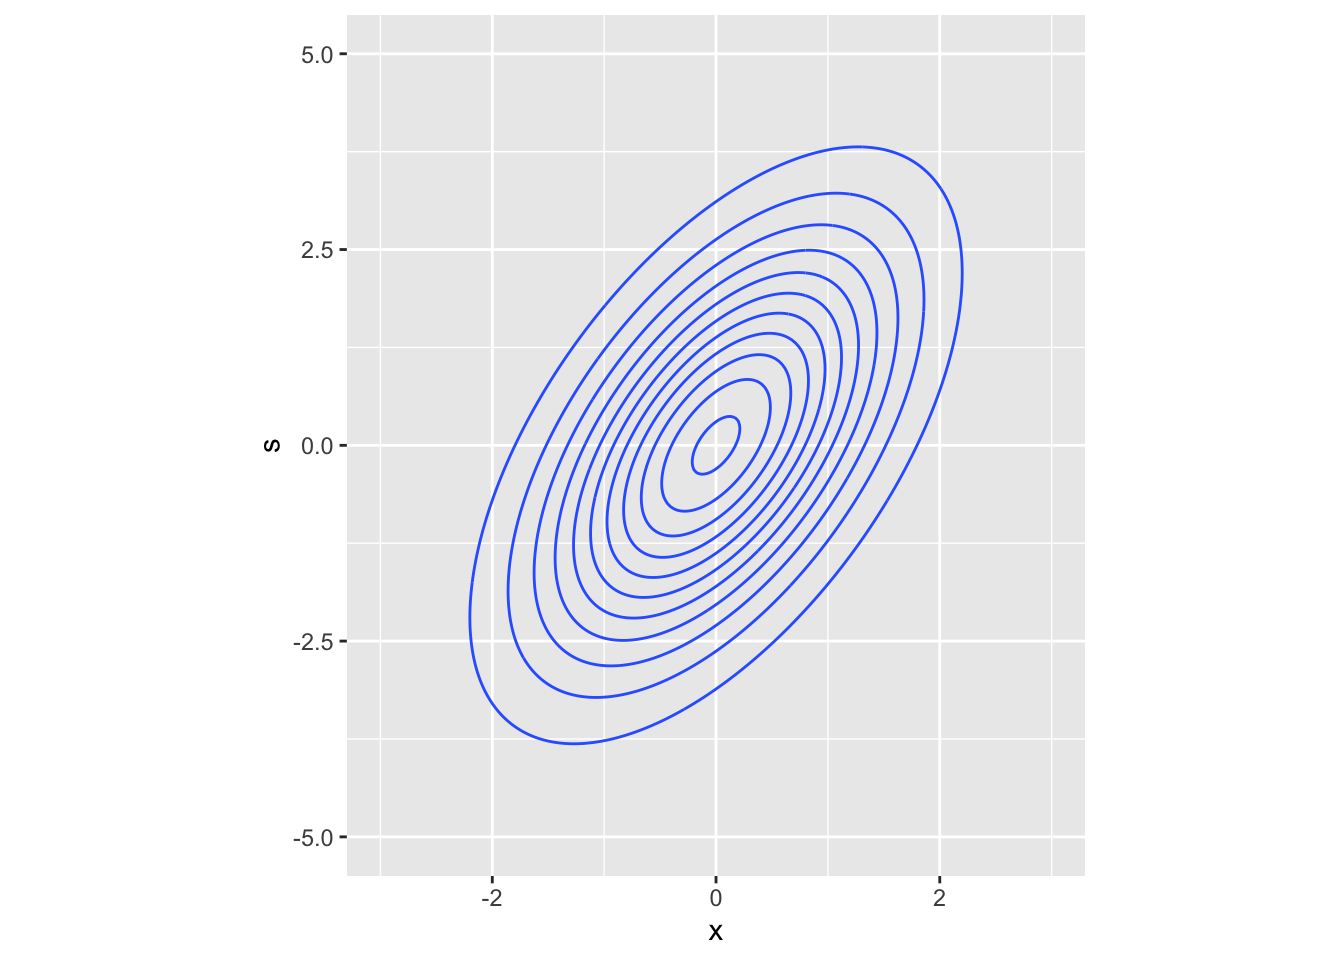
\includegraphics{smr_book_files/figure-latex/unnamed-chunk-91-1.pdf}

\subsection{Exercises}\label{exercises-1}

Take two bivariate random variables (the same as before, \(X, S\)).
Complete these tasks:

\begin{enumerate}
\def\labelenumi{\alph{enumi}.}
\tightlist
\item
  Compute \(P(X < 0 \cap S < 0)\) with \texttt{pmvnorm}
\item
  Compute \(P(X < 0 \cap S< 0)\) by simulation (Monte Carlo estimate)
\item
  Compute \(P(X > 1 \cap S < 0)\) by simulation. Can you do it with \texttt{pmvnorm}?
  (hint: check \texttt{?pmvnorm})
\end{enumerate}

\subsection{Solutions}\label{solutions}

\begin{enumerate}
\def\labelenumi{\alph{enumi}.}
\tightlist
\item
\end{enumerate}

\begin{Shaded}
\begin{Highlighting}[]
\FunctionTok{pmvnorm}\NormalTok{(}\AttributeTok{upper =} \FunctionTok{c}\NormalTok{(}\DecValTok{0}\NormalTok{, }\DecValTok{0}\NormalTok{), }\AttributeTok{mean =}\NormalTok{ m, }\AttributeTok{sigma =}\NormalTok{ vcov\_mat)}
\end{Highlighting}
\end{Shaded}

\begin{verbatim}
## [1] 0.3479566
## attr(,"error")
## [1] 1e-15
## attr(,"msg")
## [1] "Normal Completion"
\end{verbatim}

\begin{enumerate}
\def\labelenumi{\alph{enumi}.}
\setcounter{enumi}{1}
\tightlist
\item
\end{enumerate}

\begin{Shaded}
\begin{Highlighting}[]
\NormalTok{sim }\OtherTok{\textless{}{-}} \FunctionTok{rmvnorm}\NormalTok{(}\DecValTok{100000}\NormalTok{, }\AttributeTok{mean =}\NormalTok{ m, }\AttributeTok{sigma =}\NormalTok{ vcov\_mat) }\CommentTok{\# simulate enough samples}
\CommentTok{\# count all the observations satisfying the condition}
\CommentTok{\# and divide by the number of total obs to obtain a ratio}
\CommentTok{\# mean() applied to logical values is the proportion of true vars}
\FunctionTok{mean}\NormalTok{(sim[, }\DecValTok{1}\NormalTok{] }\SpecialCharTok{\textless{}} \DecValTok{0} \SpecialCharTok{\&}\NormalTok{ sim[, }\DecValTok{2}\NormalTok{] }\SpecialCharTok{\textless{}} \DecValTok{0}\NormalTok{)}
\end{Highlighting}
\end{Shaded}

\begin{verbatim}
## [1] 0.34856
\end{verbatim}

\begin{enumerate}
\def\labelenumi{\alph{enumi}.}
\setcounter{enumi}{2}
\tightlist
\item
\end{enumerate}

\begin{Shaded}
\begin{Highlighting}[]
\FunctionTok{mean}\NormalTok{(sim[, }\DecValTok{1}\NormalTok{] }\SpecialCharTok{\textgreater{}} \DecValTok{1} \SpecialCharTok{\&}\NormalTok{ sim[, }\DecValTok{2}\NormalTok{] }\SpecialCharTok{\textless{}} \DecValTok{0}\NormalTok{)}
\end{Highlighting}
\end{Shaded}

\begin{verbatim}
## [1] 0.0238
\end{verbatim}

\begin{Shaded}
\begin{Highlighting}[]
\CommentTok{\# use lower and upper limits as described in the pmvnorm docs}
\FunctionTok{pmvnorm}\NormalTok{(}\AttributeTok{lower =} \FunctionTok{c}\NormalTok{(}\DecValTok{1}\NormalTok{, }\SpecialCharTok{{-}}\ConstantTok{Inf}\NormalTok{), }\AttributeTok{upper =} \FunctionTok{c}\NormalTok{(}\ConstantTok{Inf}\NormalTok{, }\DecValTok{0}\NormalTok{), }\AttributeTok{mean =}\NormalTok{ m, }\AttributeTok{sigma =}\NormalTok{ vcov\_mat)}
\end{Highlighting}
\end{Shaded}

\begin{verbatim}
## [1] 0.0240375
## attr(,"error")
## [1] 1e-15
## attr(,"msg")
## [1] "Normal Completion"
\end{verbatim}

Increasing the Monte Carlo samples you will get a more accurate estimate
of the probability measure.

\chapter{The linear model}\label{the-linear-model}

During this lecture, we will use the \emph{Advertising} dataset,
which can be found \href{https://www.kaggle.com/datasets/ashydv/advertising-dataset}{in Kaggle}.
It shows, for each line, the revenue (\texttt{Sales}), which is the \emph{response} depending on
three \emph{predictors}, i.e.~money spent on three different advertising channels: \texttt{TV}, \texttt{Radio}, \texttt{Newspaper}.
Every variable is continuous, allowing to explain the main R
functions used in a plain linear regression task.

\section{Dataset import}\label{dataset-import}

Import the dataset (you may have to select properly the current working directory).
Remember a modern version of a dataset in R is called \emph{tibble} (as opposed to the
previous \emph{dataframe})

\begin{Shaded}
\begin{Highlighting}[]
\FunctionTok{library}\NormalTok{(readr)}
\CommentTok{\# here the wd contains a folder \textquotesingle{}dataset\textquotesingle{} which}
\CommentTok{\# in turn contains the file to be read}
\NormalTok{advertising }\OtherTok{\textless{}{-}} \FunctionTok{read\_csv}\NormalTok{(}\StringTok{"./datasets/advertising.csv"}\NormalTok{)}
\end{Highlighting}
\end{Shaded}

\begin{verbatim}
## Rows: 200 Columns: 4
## -- Column specification --------------------------------------------------------
## Delimiter: ","
## dbl (4): TV, Radio, Newspaper, Sales
## 
## i Use `spec()` to retrieve the full column specification for this data.
## i Specify the column types or set `show_col_types = FALSE` to quiet this message.
\end{verbatim}

\begin{Shaded}
\begin{Highlighting}[]
\NormalTok{advertising}
\end{Highlighting}
\end{Shaded}

\begin{verbatim}
## # A tibble: 200 x 4
##       TV Radio Newspaper Sales
##    <dbl> <dbl>     <dbl> <dbl>
##  1 230.   37.8      69.2  22.1
##  2  44.5  39.3      45.1  10.4
##  3  17.2  45.9      69.3  12  
##  4 152.   41.3      58.5  16.5
##  5 181.   10.8      58.4  17.9
##  6   8.7  48.9      75     7.2
##  7  57.5  32.8      23.5  11.8
##  8 120.   19.6      11.6  13.2
##  9   8.6   2.1       1     4.8
## 10 200.    2.6      21.2  15.6
## # i 190 more rows
\end{verbatim}

\section{Basic EDA (Exploratory Data Analysis)}\label{basic-eda-exploratory-data-analysis}

Get some basic statistics with \texttt{summary()}

\begin{Shaded}
\begin{Highlighting}[]
\FunctionTok{summary}\NormalTok{(advertising)}
\end{Highlighting}
\end{Shaded}

\begin{verbatim}
##        TV             Radio          Newspaper          Sales      
##  Min.   :  0.70   Min.   : 0.000   Min.   :  0.30   Min.   : 1.60  
##  1st Qu.: 74.38   1st Qu.: 9.975   1st Qu.: 12.75   1st Qu.:11.00  
##  Median :149.75   Median :22.900   Median : 25.75   Median :16.00  
##  Mean   :147.04   Mean   :23.264   Mean   : 30.55   Mean   :15.13  
##  3rd Qu.:218.82   3rd Qu.:36.525   3rd Qu.: 45.10   3rd Qu.:19.05  
##  Max.   :296.40   Max.   :49.600   Max.   :114.00   Max.   :27.00
\end{verbatim}

You can \texttt{attach()} the dataset to access columns writing less code, although this is not
recommended nowadays (see \texttt{with()} below). All the columns of the table are then
available in the R environment without prepending the dataset name

\begin{Shaded}
\begin{Highlighting}[]
\FunctionTok{attach}\NormalTok{(advertising)}
\FunctionTok{head}\NormalTok{(TV)}
\end{Highlighting}
\end{Shaded}

\begin{verbatim}
## [1] 230.1  44.5  17.2 151.5 180.8   8.7
\end{verbatim}

To revert back, detach the dataset

\begin{Shaded}
\begin{Highlighting}[]
\FunctionTok{detach}\NormalTok{(advertising)}
\end{Highlighting}
\end{Shaded}

It is better to use \texttt{with()} instead.
This function basically attaches a certain context object
(e.g.~the dataset namespace), executes the commands inside
the curly brackets, and then detaches the context object.

\begin{Shaded}
\begin{Highlighting}[]
\FunctionTok{with}\NormalTok{(advertising, \{}
  \FunctionTok{print}\NormalTok{(}\FunctionTok{head}\NormalTok{(Sales))}
  \FunctionTok{print}\NormalTok{(}\FunctionTok{mean}\NormalTok{(TV))}
  \FunctionTok{print}\NormalTok{(Radio[Radio }\SpecialCharTok{\textless{}} \DecValTok{20}\NormalTok{])}
\NormalTok{\})}
\end{Highlighting}
\end{Shaded}

\begin{verbatim}
## [1] 22.1 10.4 12.0 16.5 17.9  7.2
## [1] 147.0425
##  [1] 10.8 19.6  2.1  2.6  5.8  7.6  5.1 15.9 16.9 12.6  3.5 16.7 16.0 17.4  1.5
## [16]  1.4  4.1  8.4  9.9 15.8 11.7  3.1  9.6 19.2  2.0 15.5  9.3 14.5 14.3  5.7
## [31]  1.6  7.7  4.1 18.4  4.9  1.5 14.0  3.5  4.3 10.1 17.2 11.0  0.3  0.4  8.2
## [46] 15.4 14.3  0.8 16.0  2.4 11.8  0.0 12.0  2.9 17.0  5.7 14.8  1.9  7.3 13.9
## [61]  8.4 11.6  1.3 18.4 18.1 18.1 14.7  3.4  5.2 10.6 11.6  7.1  3.4  7.8  2.3
## [76] 10.0  2.6  5.4  5.7  2.1 13.9 12.1 10.8  4.1  3.7  4.9  9.3  8.6
\end{verbatim}

These are some of the functions that might be useful
when gathering information about a dataset.

\begin{Shaded}
\begin{Highlighting}[]
\FunctionTok{length}\NormalTok{(advertising) }\CommentTok{\# columns!}
\end{Highlighting}
\end{Shaded}

\begin{verbatim}
## [1] 4
\end{verbatim}

\begin{Shaded}
\begin{Highlighting}[]
\FunctionTok{nrow}\NormalTok{(advertising)}
\end{Highlighting}
\end{Shaded}

\begin{verbatim}
## [1] 200
\end{verbatim}

\begin{Shaded}
\begin{Highlighting}[]
\FunctionTok{dim}\NormalTok{(advertising)}
\end{Highlighting}
\end{Shaded}

\begin{verbatim}
## [1] 200   4
\end{verbatim}

\begin{Shaded}
\begin{Highlighting}[]
\FunctionTok{names}\NormalTok{(advertising)}
\end{Highlighting}
\end{Shaded}

\begin{verbatim}
## [1] "TV"        "Radio"     "Newspaper" "Sales"
\end{verbatim}

\section{Simple plots}\label{simple-plots}

When exploring a dataset, \texttt{ggplot()} might be a bit excessive
(recall that \texttt{ggplot()} is a modern way to draw cool plots using
a graphical syntax). Faster plots can be drawn with \texttt{plot()} and \texttt{pairs()}

\begin{Shaded}
\begin{Highlighting}[]
\FunctionTok{plot}\NormalTok{(advertising)}
\end{Highlighting}
\end{Shaded}

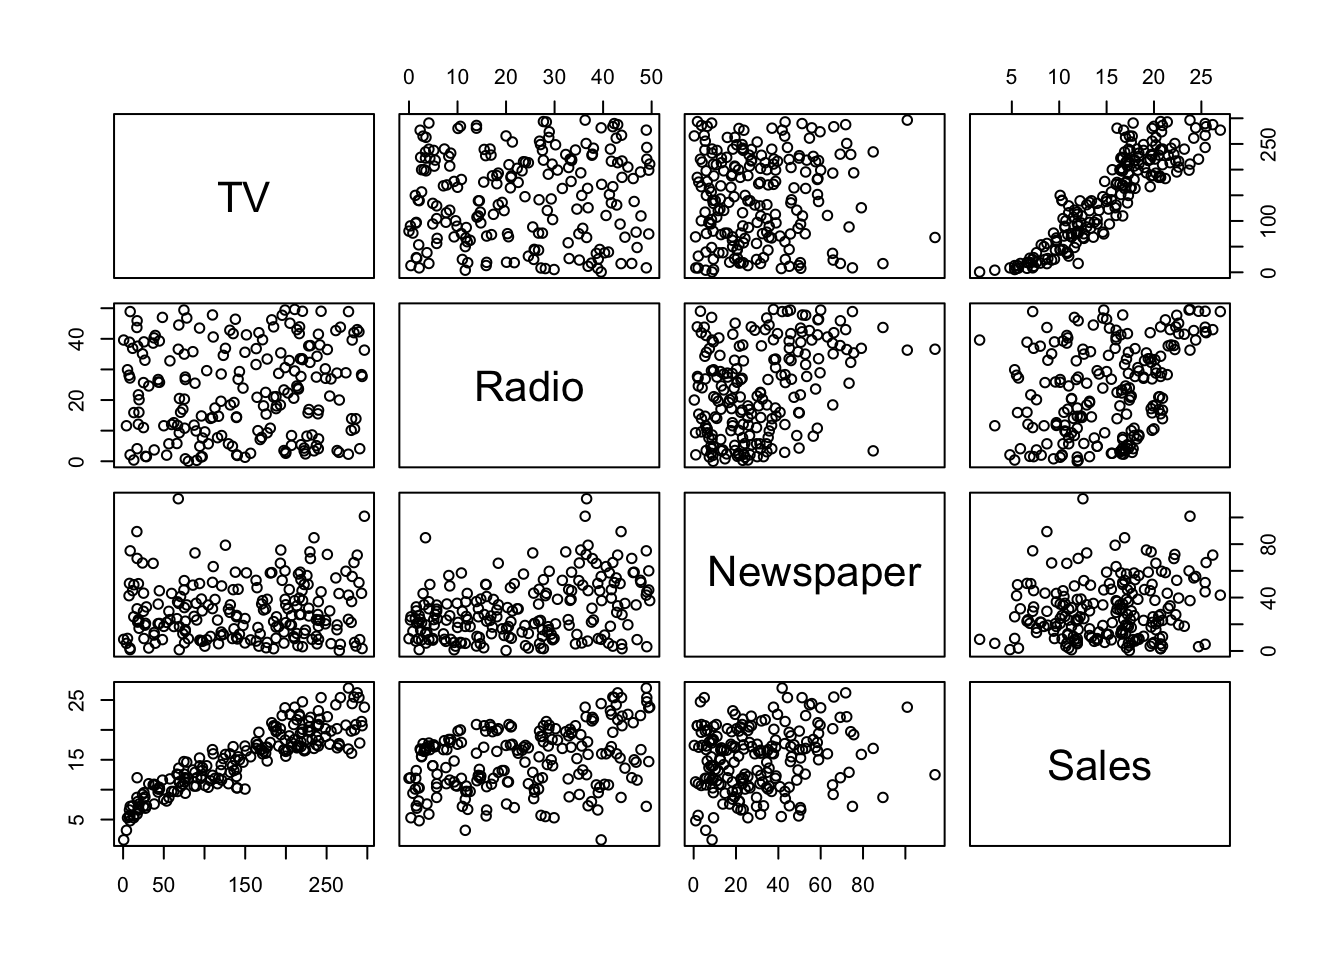
\includegraphics{smr_book_files/figure-latex/unnamed-chunk-103-1.pdf}

A pair-plot gives a bigger picture of the
cross correlations between variables.
The base R \texttt{pairs()} function can be tweaked (check \texttt{?pairs})
in order to draw other kind of information of interest.

\begin{Shaded}
\begin{Highlighting}[]
\DocumentationTok{\#\# put histograms on the diagonal}
\NormalTok{panel\_hist }\OtherTok{\textless{}{-}} \ControlFlowTok{function}\NormalTok{(x, ...) \{}
\NormalTok{  usr }\OtherTok{\textless{}{-}} \FunctionTok{par}\NormalTok{(}\StringTok{"usr"}\NormalTok{)}
  \FunctionTok{par}\NormalTok{(}\AttributeTok{usr =} \FunctionTok{c}\NormalTok{(usr[}\DecValTok{1}\SpecialCharTok{:}\DecValTok{2}\NormalTok{], }\DecValTok{0}\NormalTok{, }\FloatTok{1.5}\NormalTok{))}
\NormalTok{  h }\OtherTok{\textless{}{-}} \FunctionTok{hist}\NormalTok{(x, }\AttributeTok{plot =} \ConstantTok{FALSE}\NormalTok{)}
\NormalTok{  breaks }\OtherTok{\textless{}{-}}\NormalTok{ h}\SpecialCharTok{$}\NormalTok{breaks}
\NormalTok{  nb }\OtherTok{\textless{}{-}} \FunctionTok{length}\NormalTok{(breaks)}
\NormalTok{  y }\OtherTok{\textless{}{-}}\NormalTok{ h}\SpecialCharTok{$}\NormalTok{counts}
\NormalTok{  y }\OtherTok{\textless{}{-}}\NormalTok{ y }\SpecialCharTok{/} \FunctionTok{max}\NormalTok{(y)}
  \FunctionTok{rect}\NormalTok{(breaks[}\SpecialCharTok{{-}}\NormalTok{nb], }\DecValTok{0}\NormalTok{, breaks[}\SpecialCharTok{{-}}\DecValTok{1}\NormalTok{], y, }\AttributeTok{col =} \StringTok{"cyan"}\NormalTok{, ...)}
\NormalTok{\}}
\DocumentationTok{\#\# put (absolute) correlations on the upper panels,}
\DocumentationTok{\#\# with size proportional to the correlations.}
\NormalTok{panel\_cor }\OtherTok{\textless{}{-}} \ControlFlowTok{function}\NormalTok{(x, y, }\AttributeTok{digits =} \DecValTok{2}\NormalTok{, }\AttributeTok{prefix =} \StringTok{""}\NormalTok{, cex\_cor, ...) \{}
  \FunctionTok{par}\NormalTok{(}\AttributeTok{usr =} \FunctionTok{c}\NormalTok{(}\DecValTok{0}\NormalTok{, }\DecValTok{1}\NormalTok{, }\DecValTok{0}\NormalTok{, }\DecValTok{1}\NormalTok{))}
\NormalTok{  r }\OtherTok{\textless{}{-}} \FunctionTok{abs}\NormalTok{(}\FunctionTok{cor}\NormalTok{(x, y))}
\NormalTok{  txt }\OtherTok{\textless{}{-}} \FunctionTok{format}\NormalTok{(}\FunctionTok{c}\NormalTok{(r, }\FloatTok{0.123456789}\NormalTok{), }\AttributeTok{digits =}\NormalTok{ digits)[}\DecValTok{1}\NormalTok{]}
\NormalTok{  txt }\OtherTok{\textless{}{-}} \FunctionTok{paste0}\NormalTok{(prefix, txt)}
  \ControlFlowTok{if}\NormalTok{ (}\FunctionTok{missing}\NormalTok{(cex\_cor)) cex\_cor }\OtherTok{\textless{}{-}} \FloatTok{0.8} \SpecialCharTok{/} \FunctionTok{strwidth}\NormalTok{(txt)}
  \FunctionTok{text}\NormalTok{(}\FloatTok{0.5}\NormalTok{, }\FloatTok{0.5}\NormalTok{, txt, }\AttributeTok{cex =}\NormalTok{ cex\_cor }\SpecialCharTok{*}\NormalTok{ r)}
\NormalTok{\}}

\FunctionTok{pairs}\NormalTok{(advertising,}
  \AttributeTok{upper.panel =}\NormalTok{ panel\_cor, }\AttributeTok{diag.panel =}\NormalTok{ panel\_hist}
\NormalTok{)}
\end{Highlighting}
\end{Shaded}

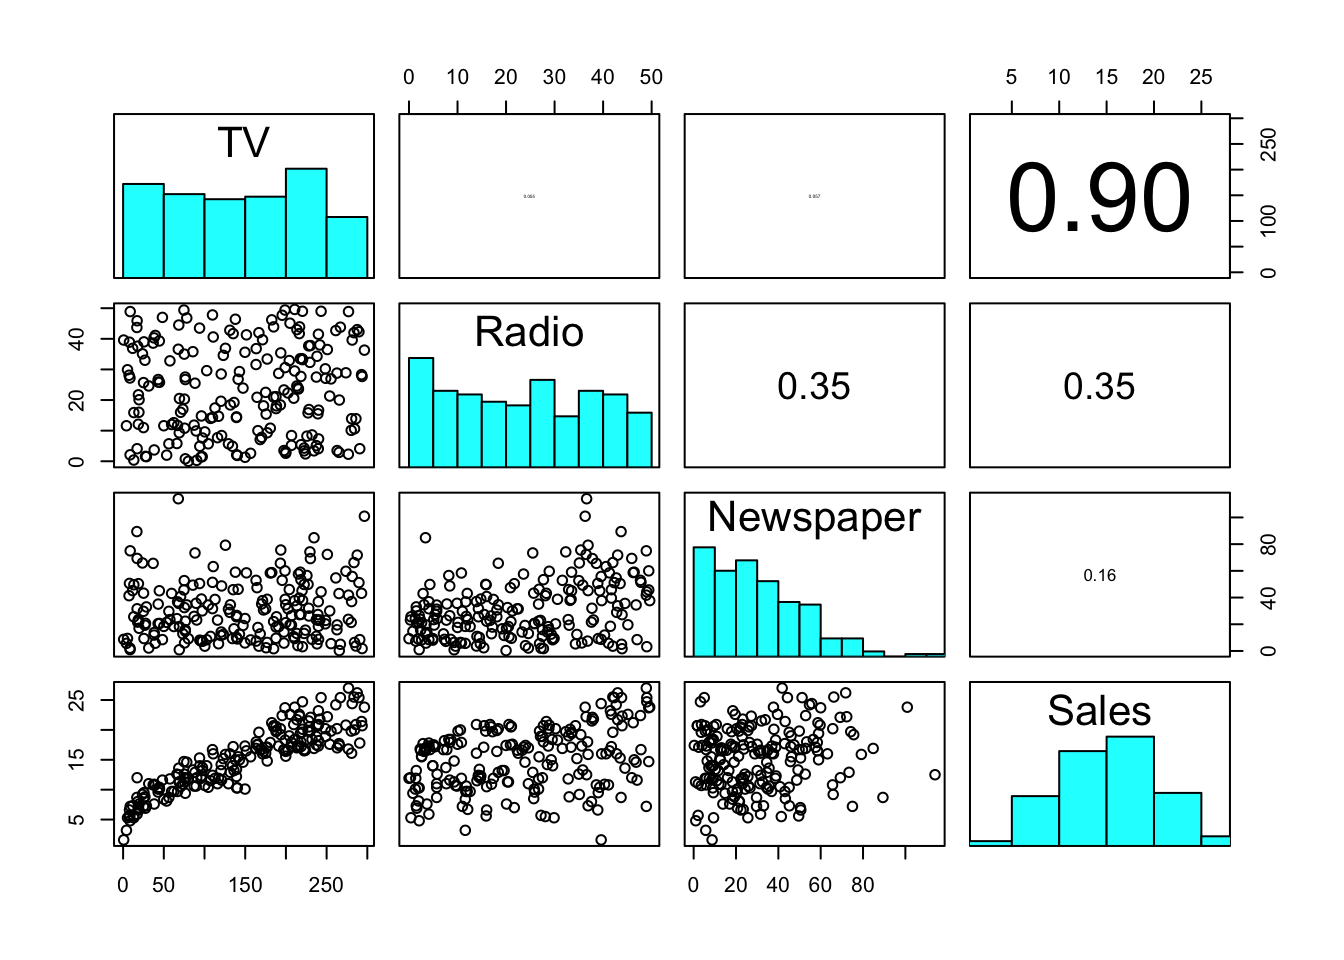
\includegraphics{smr_book_files/figure-latex/unnamed-chunk-104-1.pdf}

With much less effort, we can obtain a prettier
version of the pair-plot.

\begin{Shaded}
\begin{Highlighting}[]
\FunctionTok{library}\NormalTok{(GGally)}
\end{Highlighting}
\end{Shaded}

\begin{verbatim}
## Registered S3 method overwritten by 'GGally':
##   method from   
##   +.gg   ggplot2
\end{verbatim}

\begin{Shaded}
\begin{Highlighting}[]
\FunctionTok{ggpairs}\NormalTok{(advertising, }\AttributeTok{progress =} \ConstantTok{FALSE}\NormalTok{)}
\end{Highlighting}
\end{Shaded}

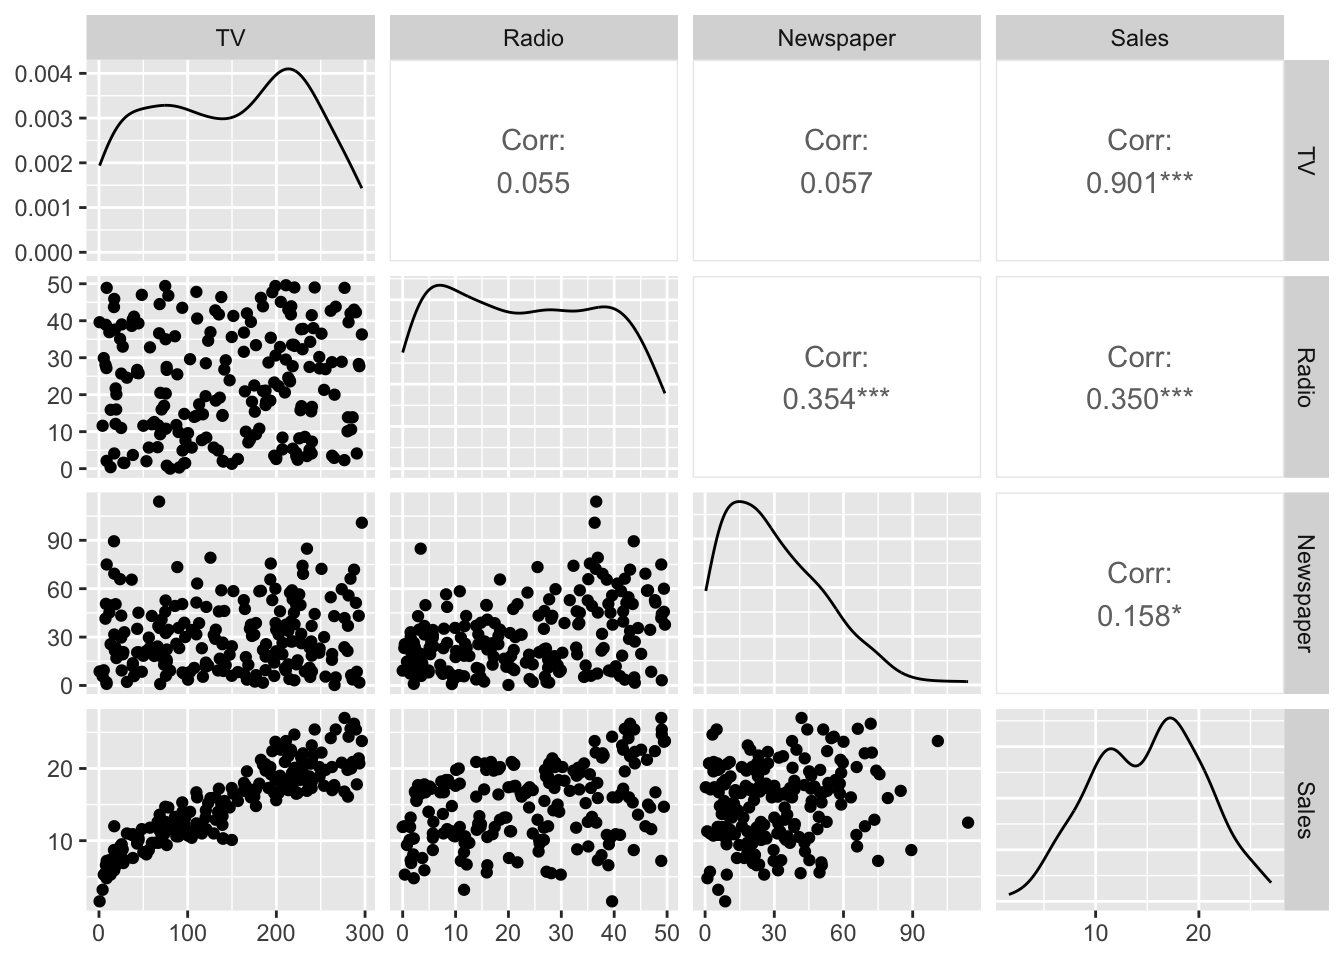
\includegraphics{smr_book_files/figure-latex/unnamed-chunk-105-1.pdf}

Again, with base R let's plot the predictors against the response.
We know how to do that with a single predictor.

\begin{Shaded}
\begin{Highlighting}[]
\FunctionTok{plot}\NormalTok{(advertising}\SpecialCharTok{$}\NormalTok{TV, advertising}\SpecialCharTok{$}\NormalTok{Sales)}
\end{Highlighting}
\end{Shaded}

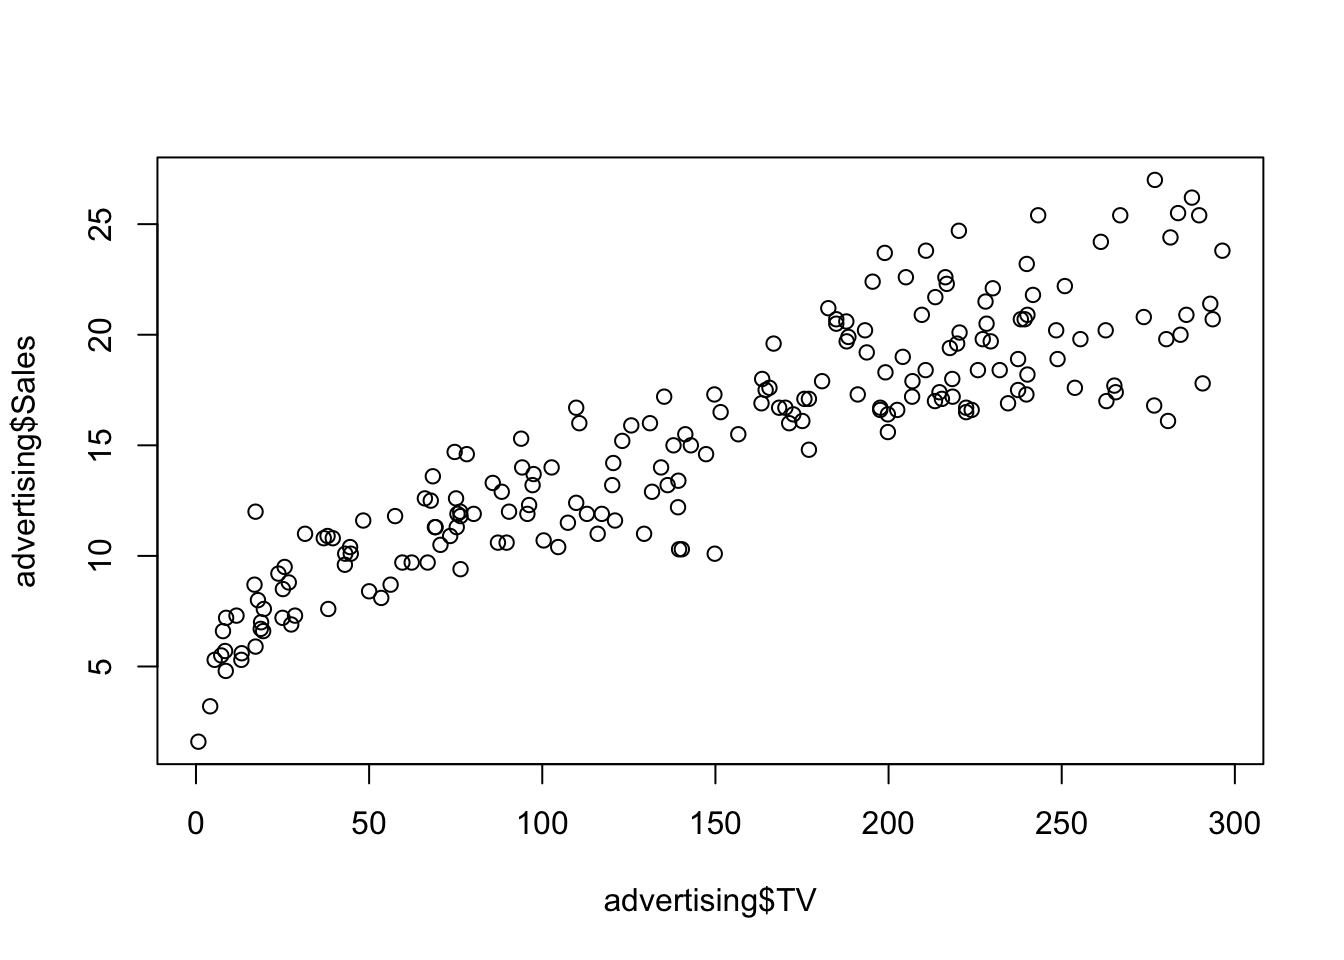
\includegraphics{smr_book_files/figure-latex/unnamed-chunk-106-1.pdf}

In case we want to add all plots to a single figure,
we can do it as follow (base R)

\begin{Shaded}
\begin{Highlighting}[]
\CommentTok{\# set plot parameters}
\FunctionTok{with}\NormalTok{(advertising, \{}
  \FunctionTok{par}\NormalTok{(}\AttributeTok{mfrow =} \FunctionTok{c}\NormalTok{(}\DecValTok{1}\NormalTok{, }\DecValTok{3}\NormalTok{))}
  \FunctionTok{plot}\NormalTok{(TV, Sales)}
  \FunctionTok{plot}\NormalTok{(Radio, Sales)}
  \FunctionTok{plot}\NormalTok{(Newspaper, Sales)}
\NormalTok{\})}
\end{Highlighting}
\end{Shaded}

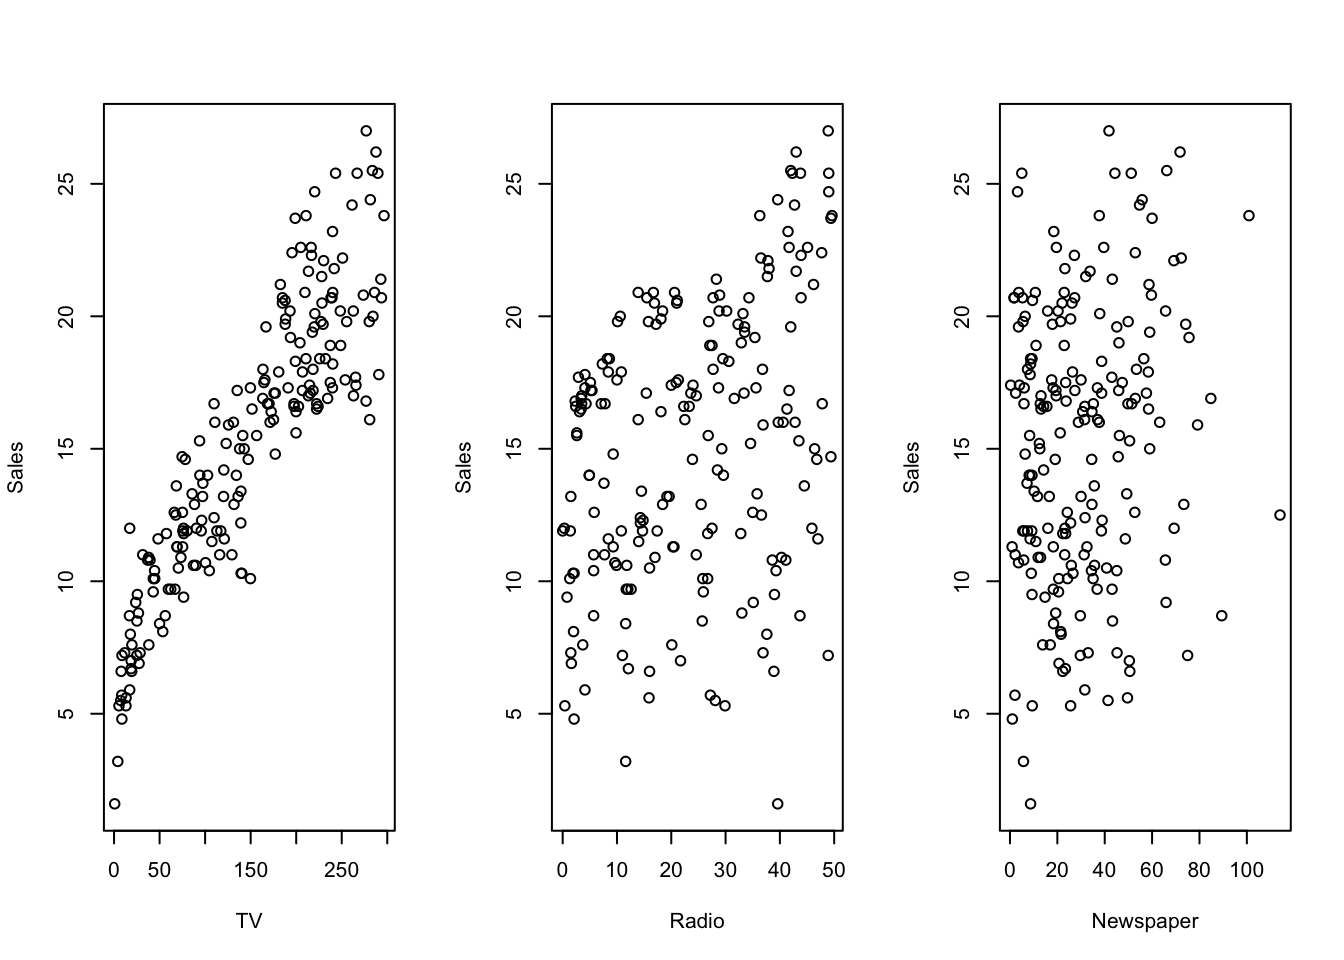
\includegraphics{smr_book_files/figure-latex/unnamed-chunk-107-1.pdf}

adding a smoothed line would look like this

\begin{Shaded}
\begin{Highlighting}[]
\CommentTok{\# set plot parameters}
\FunctionTok{with}\NormalTok{(advertising, \{}
  \FunctionTok{par}\NormalTok{(}\AttributeTok{mfrow =} \FunctionTok{c}\NormalTok{(}\DecValTok{1}\NormalTok{, }\DecValTok{3}\NormalTok{))}
  \FunctionTok{scatter.smooth}\NormalTok{(TV, Sales, }\AttributeTok{col =} \StringTok{"red"}\NormalTok{)}
  \FunctionTok{scatter.smooth}\NormalTok{(Radio, Sales, }\AttributeTok{col =} \StringTok{"red"}\NormalTok{)}
  \FunctionTok{scatter.smooth}\NormalTok{(Newspaper, Sales, }\AttributeTok{col =} \StringTok{"red"}\NormalTok{, }\AttributeTok{span =}\NormalTok{ .}\DecValTok{3}\NormalTok{) }\CommentTok{\# tweak with span}
\NormalTok{\})}
\end{Highlighting}
\end{Shaded}

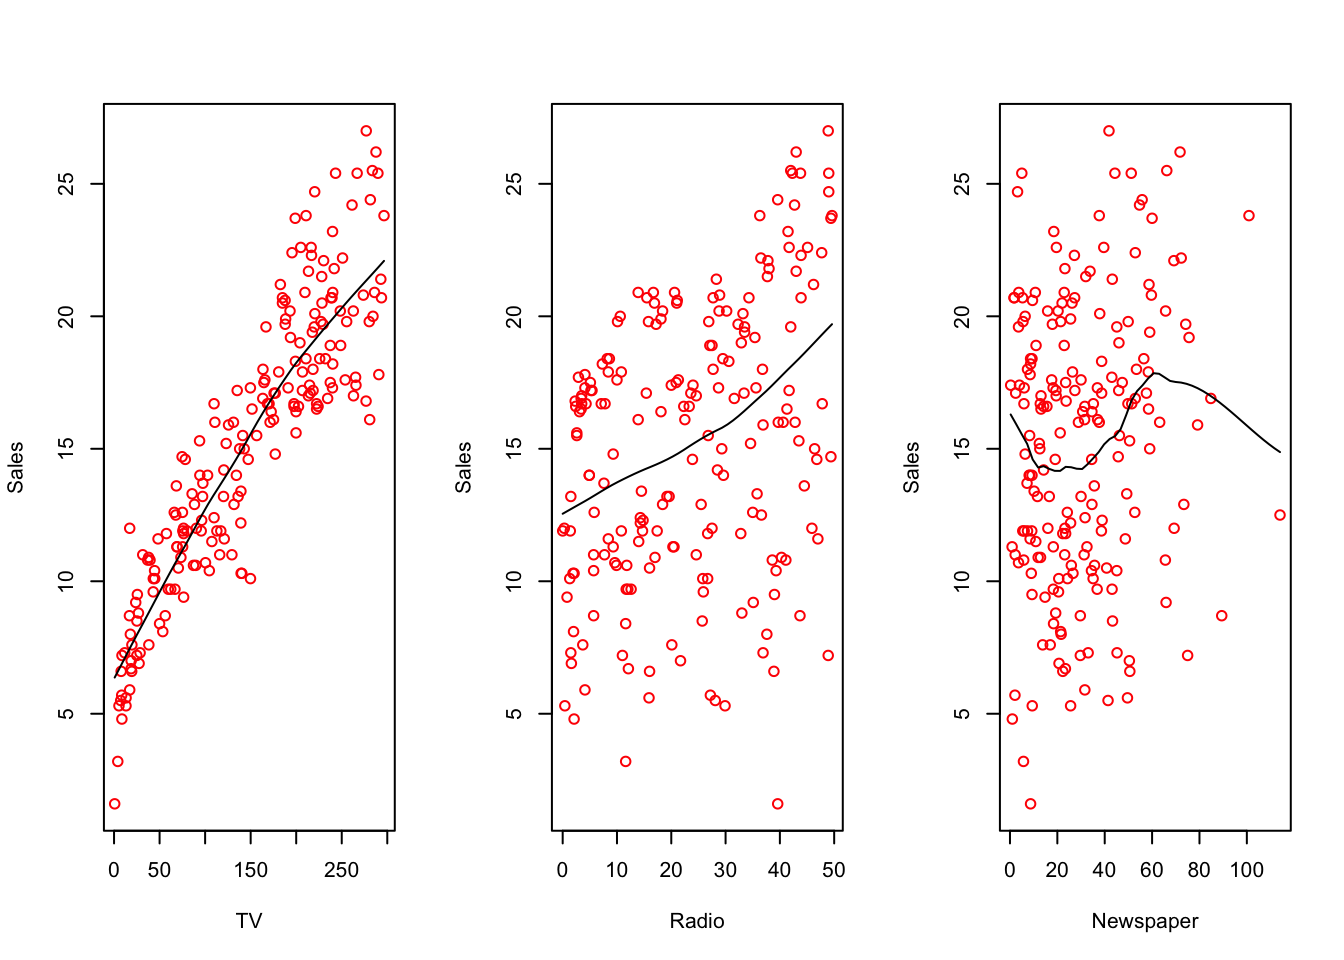
\includegraphics{smr_book_files/figure-latex/unnamed-chunk-108-1.pdf}

The same pictures can also be plotted with \texttt{ggplot()},
if preferred (in two ways).

\begin{Shaded}
\begin{Highlighting}[]
\FunctionTok{library}\NormalTok{(ggplot2)}

\FunctionTok{ggplot}\NormalTok{(advertising) }\SpecialCharTok{+}
  \FunctionTok{geom\_point}\NormalTok{(}\FunctionTok{aes}\NormalTok{(TV, Sales))}
\end{Highlighting}
\end{Shaded}

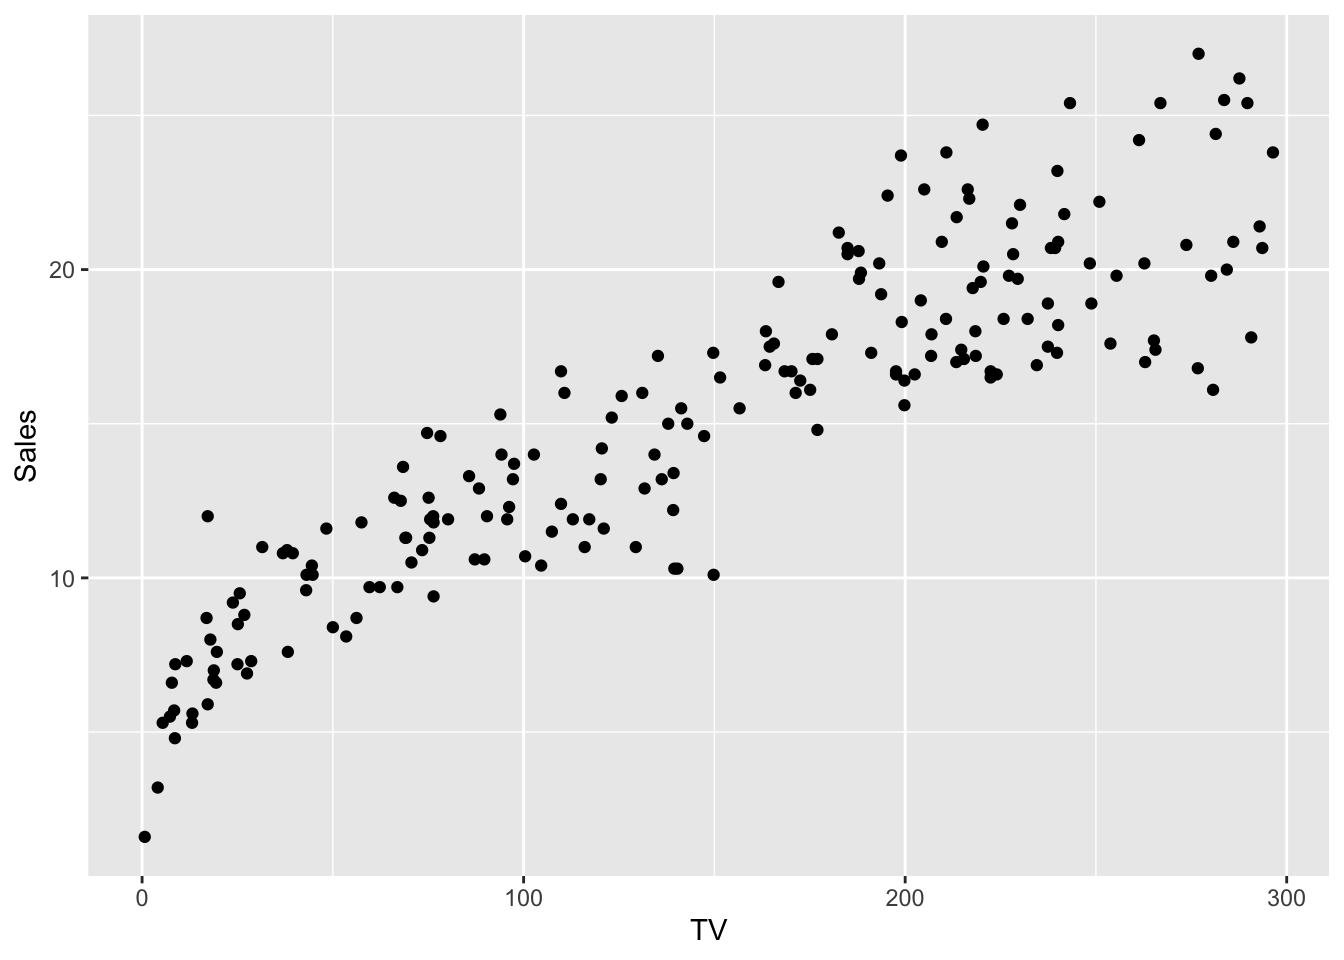
\includegraphics{smr_book_files/figure-latex/unnamed-chunk-109-1.pdf}

First method: draw three separate plots and arrange
them together with \texttt{ggarrange()}

\begin{Shaded}
\begin{Highlighting}[]
\FunctionTok{library}\NormalTok{(ggpubr)}
\NormalTok{tvplt }\OtherTok{\textless{}{-}} \FunctionTok{ggplot}\NormalTok{(advertising, }\AttributeTok{mapping =} \FunctionTok{aes}\NormalTok{(TV, Sales)) }\SpecialCharTok{+}
  \FunctionTok{geom\_point}\NormalTok{() }\SpecialCharTok{+}
  \FunctionTok{geom\_smooth}\NormalTok{()}
\NormalTok{radplt }\OtherTok{\textless{}{-}} \FunctionTok{ggplot}\NormalTok{(advertising, }\AttributeTok{mapping =} \FunctionTok{aes}\NormalTok{(Radio, Sales)) }\SpecialCharTok{+}
  \FunctionTok{geom\_point}\NormalTok{() }\SpecialCharTok{+}
  \FunctionTok{geom\_smooth}\NormalTok{()}
\NormalTok{nwsplt }\OtherTok{\textless{}{-}} \FunctionTok{ggplot}\NormalTok{(advertising, }\AttributeTok{mapping =} \FunctionTok{aes}\NormalTok{(Newspaper, Sales)) }\SpecialCharTok{+}
  \FunctionTok{geom\_point}\NormalTok{() }\SpecialCharTok{+}
  \FunctionTok{geom\_smooth}\NormalTok{()}

\FunctionTok{ggarrange}\NormalTok{(tvplt, radplt, nwsplt,}
  \AttributeTok{ncol =} \DecValTok{3}
\NormalTok{)}
\end{Highlighting}
\end{Shaded}

\begin{verbatim}
## `geom_smooth()` using method = 'loess' and formula = 'y ~ x'
## `geom_smooth()` using method = 'loess' and formula = 'y ~ x'
## `geom_smooth()` using method = 'loess' and formula = 'y ~ x'
\end{verbatim}

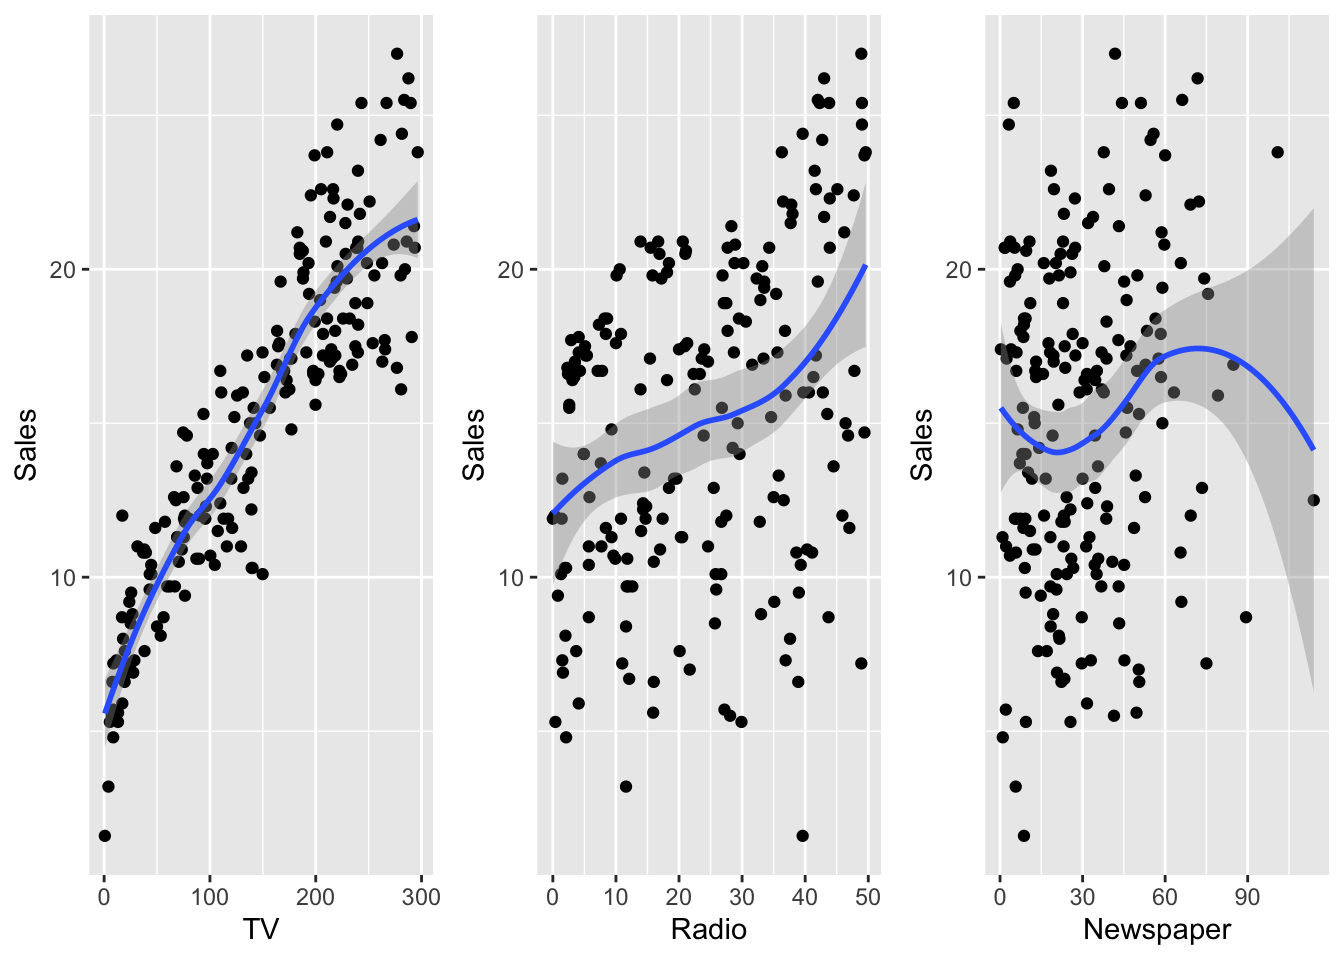
\includegraphics{smr_book_files/figure-latex/unnamed-chunk-110-1.pdf}

Second method: rearrange the dataset first,
and feed everything to \texttt{ggplot()}.

\begin{Shaded}
\begin{Highlighting}[]
\FunctionTok{library}\NormalTok{(tibble)}
\FunctionTok{library}\NormalTok{(tidyr)}

\DocumentationTok{\#\# if using melt, need to switch to data.frame}
\CommentTok{\# library(reshape2)}
\CommentTok{\# advertising \textless{}{-} as.data.frame(advertising)}
\CommentTok{\# long\_adv \textless{}{-} melt(advertising, id.vars = "Sales")}

\NormalTok{long\_adv }\OtherTok{\textless{}{-}}\NormalTok{ advertising }\SpecialCharTok{\%\textgreater{}\%}
  \FunctionTok{gather}\NormalTok{(channel, value, }\SpecialCharTok{{-}}\NormalTok{Sales)}
\FunctionTok{head}\NormalTok{(long\_adv)}
\end{Highlighting}
\end{Shaded}

\begin{verbatim}
## # A tibble: 6 x 3
##   Sales channel value
##   <dbl> <chr>   <dbl>
## 1  22.1 TV      230. 
## 2  10.4 TV       44.5
## 3  12   TV       17.2
## 4  16.5 TV      152. 
## 5  17.9 TV      181. 
## 6   7.2 TV        8.7
\end{verbatim}

\begin{Shaded}
\begin{Highlighting}[]
\FunctionTok{ggplot}\NormalTok{(long\_adv, }\FunctionTok{aes}\NormalTok{(value, Sales)) }\SpecialCharTok{+}
  \FunctionTok{geom\_point}\NormalTok{() }\SpecialCharTok{+}
  \FunctionTok{geom\_smooth}\NormalTok{() }\SpecialCharTok{+}
  \FunctionTok{facet\_wrap}\NormalTok{(}\SpecialCharTok{\textasciitilde{}}\NormalTok{channel, }\AttributeTok{scales =} \StringTok{"free"}\NormalTok{)}
\end{Highlighting}
\end{Shaded}

\begin{verbatim}
## `geom_smooth()` using method = 'loess' and formula = 'y ~ x'
\end{verbatim}

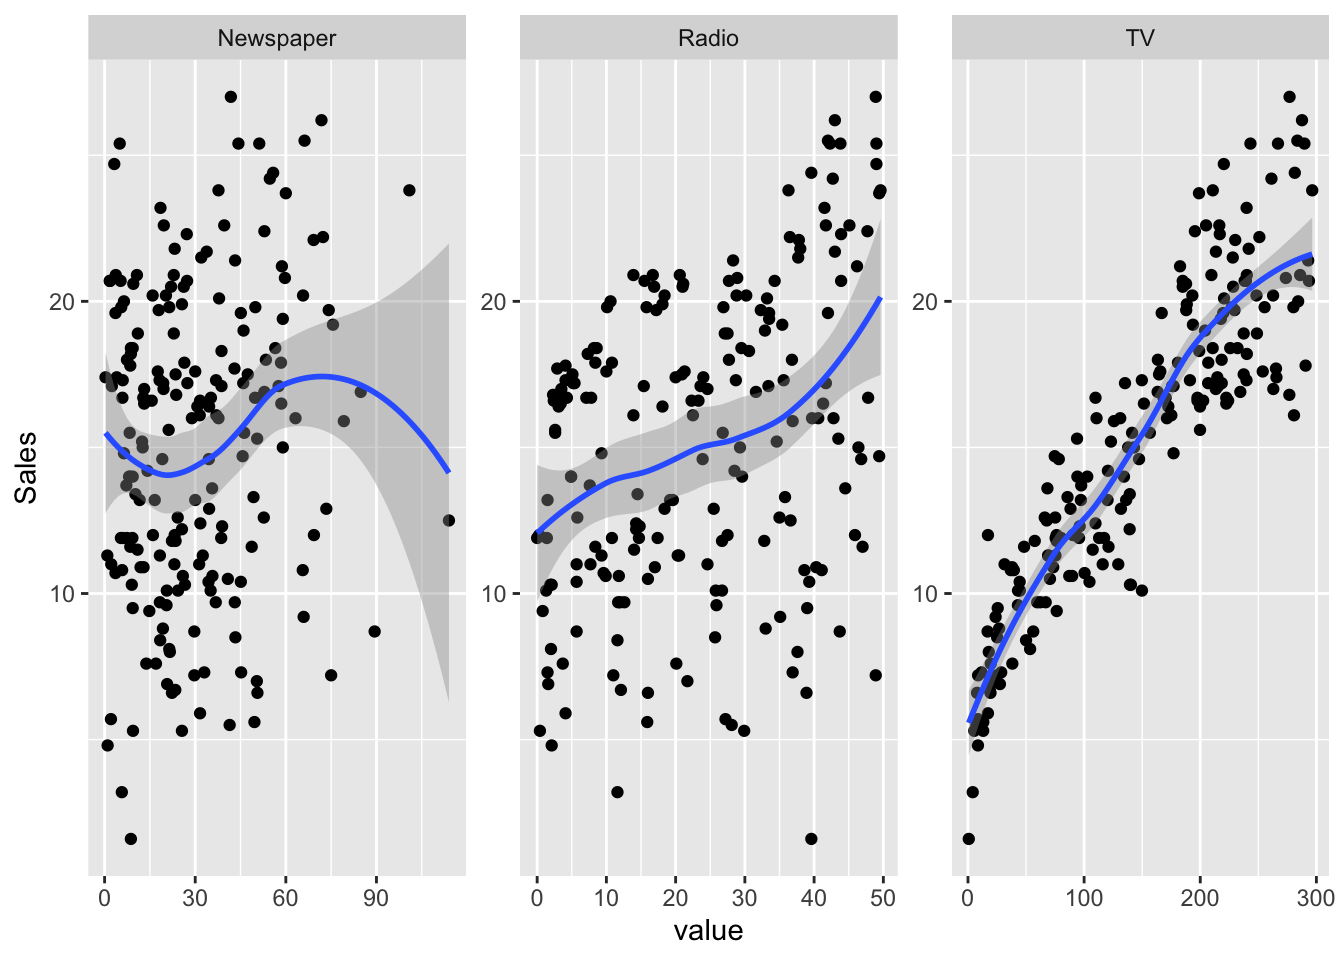
\includegraphics{smr_book_files/figure-latex/unnamed-chunk-112-1.pdf}

If you're not sure why we need to use the \texttt{melt()} function,
check the first lab (Iris dataset), or simply read the \texttt{?melt}
helper.

\section{Simple regression}\label{simple-regression}

The core of this class is the \texttt{lm()} function: its first argument is a \emph{formula},
centered around the symbol \textasciitilde, whith a response on its left and a list of predictors on its right.

Let's start with a simple single quantitative predictor linear
model (simple linear regression)

\begin{Shaded}
\begin{Highlighting}[]
\NormalTok{simple\_reg }\OtherTok{\textless{}{-}} \FunctionTok{lm}\NormalTok{(Sales }\SpecialCharTok{\textasciitilde{}}\NormalTok{ TV, }\AttributeTok{data =}\NormalTok{ advertising)}
\end{Highlighting}
\end{Shaded}

Now that we fitted the model, we have access to the
coefficient estimates and we can plot the \emph{estimated} regression
line.

\subsection{Plot}\label{plot}

Here two ways of drawing the regression line,
first in base R

\begin{Shaded}
\begin{Highlighting}[]
\FunctionTok{with}\NormalTok{(}\AttributeTok{data =}\NormalTok{ advertising, \{}
  \FunctionTok{plot}\NormalTok{(}\AttributeTok{x =}\NormalTok{ TV, }\AttributeTok{y =}\NormalTok{ Sales)}
  \CommentTok{\# abline draws a line from intercept and slope}
  \FunctionTok{abline}\NormalTok{(}
\NormalTok{    simple\_reg,}
    \AttributeTok{col =} \StringTok{"red"}
\NormalTok{  )}
\NormalTok{\})}
\end{Highlighting}
\end{Shaded}

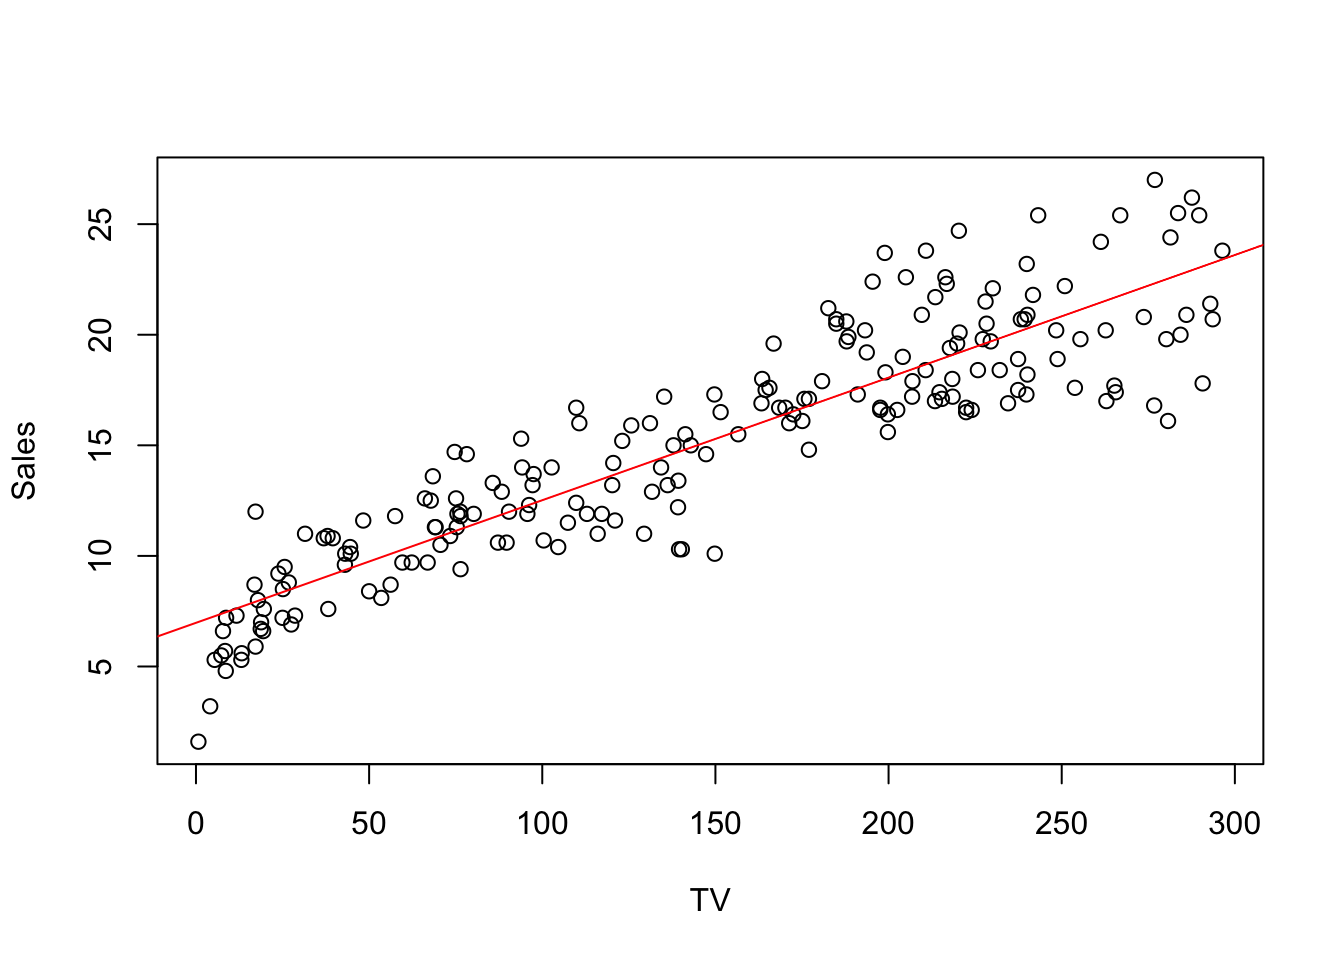
\includegraphics{smr_book_files/figure-latex/unnamed-chunk-114-1.pdf}

and in ggplot

\begin{Shaded}
\begin{Highlighting}[]
\FunctionTok{ggplot}\NormalTok{(simple\_reg, }\AttributeTok{mapping =} \FunctionTok{aes}\NormalTok{(TV, Sales)) }\SpecialCharTok{+}
  \FunctionTok{geom\_point}\NormalTok{() }\SpecialCharTok{+}
  \FunctionTok{geom\_smooth}\NormalTok{(}\AttributeTok{method =} \StringTok{"lm"}\NormalTok{, }\AttributeTok{color =} \StringTok{"red"}\NormalTok{)}
\end{Highlighting}
\end{Shaded}

\begin{verbatim}
## `geom_smooth()` using formula = 'y ~ x'
\end{verbatim}

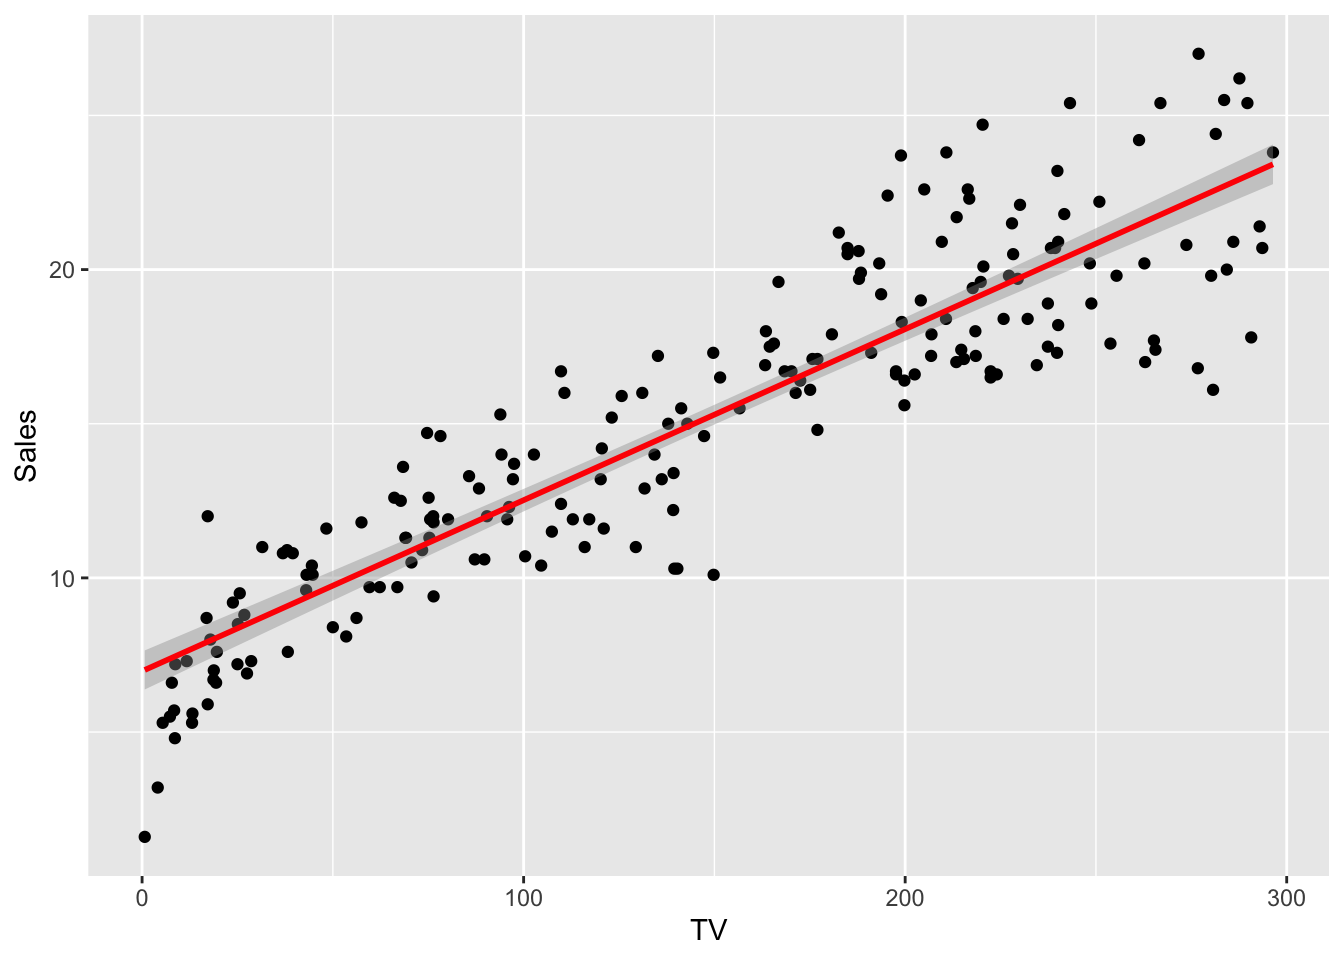
\includegraphics{smr_book_files/figure-latex/unnamed-chunk-115-1.pdf}

Actually, \texttt{lm()} does a lot more than just compute the least squares coefficients.

\begin{Shaded}
\begin{Highlighting}[]
\FunctionTok{summary}\NormalTok{(simple\_reg)}
\end{Highlighting}
\end{Shaded}

\begin{verbatim}
## 
## Call:
## lm(formula = Sales ~ TV, data = advertising)
## 
## Residuals:
##     Min      1Q  Median      3Q     Max 
## -6.4438 -1.4857  0.0218  1.5042  5.6932 
## 
## Coefficients:
##             Estimate Std. Error t value Pr(>|t|)    
## (Intercept) 6.974821   0.322553   21.62   <2e-16 ***
## TV          0.055465   0.001896   29.26   <2e-16 ***
## ---
## Signif. codes:  0 '***' 0.001 '**' 0.01 '*' 0.05 '.' 0.1 ' ' 1
## 
## Residual standard error: 2.296 on 198 degrees of freedom
## Multiple R-squared:  0.8122, Adjusted R-squared:  0.8112 
## F-statistic: 856.2 on 1 and 198 DF,  p-value: < 2.2e-16
\end{verbatim}

We will analyze in detail this output in the next subsection.

\subsection{Summary}\label{summary}

\texttt{summary(lm)} contains information about the following quantities:

\begin{itemize}
\item
  residuals: \(Y - X\hat\beta\)
\item
  estimated coefficients: \(\hat\beta\)
\item
  (estimated) standard errors on the coefficients (in the \texttt{Std.\ Error} column) \(S \sqrt{(X'X)^{-1}_{i+1,i+1}}\)
  because \(\frac{\hat\beta_i - \beta_i}{S\sqrt{(X'X)^{-1}}}\sim t(n-p)\)
\item
  in the \texttt{t\ value} column: value of the test statistic for the null hypothesis \(H_0: \beta_{i+1} = 0\)
\item
  in the \texttt{Pr(\textgreater{}\textbar{}t\textbar{})} column: p-value regarding the null hypothesis above
\item
  residual std error: \(S = \sqrt{\frac{e'e}{n-p}}\), i.e.~the square root of the Mean Square Residual (MSR)
\item
  multiple R squared: \emph{later}
\item
  adj R squared: \emph{later}
\end{itemize}

Let's compute them to make sure we understood the concepts

\subsubsection{Residuals}\label{residuals}

Easy to retrieve them (actually,
they are the realization of the residuals)

\[
e = y - X\hat\beta
\]

\begin{Shaded}
\begin{Highlighting}[]
\NormalTok{y }\OtherTok{\textless{}{-}}\NormalTok{ advertising}\SpecialCharTok{$}\NormalTok{Sales}
\NormalTok{x }\OtherTok{\textless{}{-}} \FunctionTok{cbind}\NormalTok{(}\DecValTok{1}\NormalTok{, advertising}\SpecialCharTok{$}\NormalTok{TV)}
\NormalTok{e }\OtherTok{\textless{}{-}}\NormalTok{ y }\SpecialCharTok{{-}}\NormalTok{ x }\SpecialCharTok{\%*\%}\NormalTok{ simple\_reg}\SpecialCharTok{$}\NormalTok{coefficients}
\FunctionTok{head}\NormalTok{(}\FunctionTok{tibble}\NormalTok{(}
  \AttributeTok{lm\_res =}\NormalTok{ simple\_reg}\SpecialCharTok{$}\NormalTok{residuals,}
  \AttributeTok{manual\_res =} \FunctionTok{as.vector}\NormalTok{(e)}
\NormalTok{))}
\end{Highlighting}
\end{Shaded}

\begin{verbatim}
## # A tibble: 6 x 2
##   lm_res manual_res
##    <dbl>      <dbl>
## 1  2.36       2.36 
## 2  0.957      0.957
## 3  4.07       4.07 
## 4  1.12       1.12 
## 5  0.897      0.897
## 6 -0.257     -0.257
\end{verbatim}

\subsubsection{Estimate}\label{estimate}

Estimates are just the \(\hat\beta\) values for each predictor (plus intercept).
They are computed with the closed form max likelihood formula.

\[
\hat\beta = (X'X)^{-1}X'Y
\]

\begin{Shaded}
\begin{Highlighting}[]
\NormalTok{beta\_hat }\OtherTok{\textless{}{-}} \FunctionTok{solve}\NormalTok{(}\FunctionTok{t}\NormalTok{(x) }\SpecialCharTok{\%*\%}\NormalTok{ x) }\SpecialCharTok{\%*\%} \FunctionTok{t}\NormalTok{(x) }\SpecialCharTok{\%*\%}\NormalTok{ y}
\FunctionTok{head}\NormalTok{(}\FunctionTok{tibble}\NormalTok{(}
  \AttributeTok{lm\_coeff =}\NormalTok{ simple\_reg}\SpecialCharTok{$}\NormalTok{coefficients,}
  \AttributeTok{manual\_coeff =} \FunctionTok{as.vector}\NormalTok{(beta\_hat)}
\NormalTok{))}
\end{Highlighting}
\end{Shaded}

\begin{verbatim}
## # A tibble: 2 x 2
##   lm_coeff manual_coeff
##      <dbl>        <dbl>
## 1   6.97         6.97  
## 2   0.0555       0.0555
\end{verbatim}

\subsubsection{Standard Error}\label{standard-error}

For each predictor, this quantifies the estimated variation in the beta estimator.
The lower the standard error is, the higher is the accuracy of that particular coefficient.
For predictor \(i\), it is computed as

\[
SE_i = S \sqrt{(X'X)^{-1}_{i+1,i+1}}
\]
\(i+1\) is used here since first column if for the intercept \(\beta_0\).

\begin{Shaded}
\begin{Highlighting}[]
\NormalTok{n }\OtherTok{\textless{}{-}} \FunctionTok{nrow}\NormalTok{(x)}
\NormalTok{p }\OtherTok{\textless{}{-}} \FunctionTok{ncol}\NormalTok{(x)}
\NormalTok{rms }\OtherTok{\textless{}{-}} \FunctionTok{t}\NormalTok{(e) }\SpecialCharTok{\%*\%}\NormalTok{ e }\SpecialCharTok{/}\NormalTok{ (n }\SpecialCharTok{{-}}\NormalTok{ p)}

\CommentTok{\# SE for TV}
\NormalTok{tv\_se }\OtherTok{\textless{}{-}} \FunctionTok{sqrt}\NormalTok{(rms }\SpecialCharTok{*} \FunctionTok{solve}\NormalTok{(}\FunctionTok{t}\NormalTok{(x) }\SpecialCharTok{\%*\%}\NormalTok{ x)[}\DecValTok{2}\NormalTok{, }\DecValTok{2}\NormalTok{])}
\NormalTok{tv\_se}
\end{Highlighting}
\end{Shaded}

\begin{verbatim}
##             [,1]
## [1,] 0.001895551
\end{verbatim}

\subsubsection{T-value and p-value}\label{t-value-and-p-value}

These two are related to each other. The first is the
test statistics value, under the null hypothesis
\(H_0 : \beta_i = 0\), for the variable

\[
\frac{\hat\beta_i - \beta_i}{S \sqrt{(X'X)^{-1}}}
\]

which is student-T distributed with \(n-2\) degrees of freedom.

\begin{Shaded}
\begin{Highlighting}[]
\CommentTok{\# for TV}
\NormalTok{t\_val }\OtherTok{\textless{}{-}}\NormalTok{ simple\_reg}\SpecialCharTok{$}\NormalTok{coefficients[}\DecValTok{2}\NormalTok{] }\SpecialCharTok{/}\NormalTok{ tv\_se}
\NormalTok{t\_val}
\end{Highlighting}
\end{Shaded}

\begin{verbatim}
##         [,1]
## [1,] 29.2605
\end{verbatim}

And finally, the p-value is the probability
on a \(t(n-2)\) distribution of the statistic to be
beyond the value actually observed. Remember that with \emph{beyond}
we mean on both sides of the distribution, since the
alternative hypothesis \(H_1: \beta \neq 0\) is two-sided.

\begin{Shaded}
\begin{Highlighting}[]
\CommentTok{\# multiply by two because the alternative hyp is two{-}sided}
\NormalTok{p\_val }\OtherTok{\textless{}{-}} \DecValTok{2} \SpecialCharTok{*} \FunctionTok{pt}\NormalTok{(t\_val, n }\SpecialCharTok{{-}} \DecValTok{2}\NormalTok{, }\AttributeTok{lower.tail =} \ConstantTok{FALSE}\NormalTok{)}
\NormalTok{p\_val}
\end{Highlighting}
\end{Shaded}

\begin{verbatim}
##              [,1]
## [1,] 7.927912e-74
\end{verbatim}

Here we cannot appreciate the manual computation since the
p-value is very low (meaning that we can reject the null,
favoring the alternative).

Exercise: You can try to compute this value manually on another
simple regression model where we use \texttt{Radio} as predictor.

\begin{Shaded}
\begin{Highlighting}[]
\NormalTok{radio\_simple\_reg }\OtherTok{\textless{}{-}} \FunctionTok{lm}\NormalTok{(Sales }\SpecialCharTok{\textasciitilde{}}\NormalTok{ Radio, }\AttributeTok{data =}\NormalTok{ advertising)}
\FunctionTok{summary}\NormalTok{(radio\_simple\_reg)}
\end{Highlighting}
\end{Shaded}

\begin{verbatim}
## 
## Call:
## lm(formula = Sales ~ Radio, data = advertising)
## 
## Residuals:
##      Min       1Q   Median       3Q      Max 
## -15.5632  -3.5293   0.6714   4.2504   8.6796 
## 
## Coefficients:
##             Estimate Std. Error t value Pr(>|t|)    
## (Intercept)  12.2357     0.6535  18.724  < 2e-16 ***
## Radio         0.1244     0.0237   5.251 3.88e-07 ***
## ---
## Signif. codes:  0 '***' 0.001 '**' 0.01 '*' 0.05 '.' 0.1 ' ' 1
## 
## Residual standard error: 4.963 on 198 degrees of freedom
## Multiple R-squared:  0.1222, Adjusted R-squared:  0.1178 
## F-statistic: 27.57 on 1 and 198 DF,  p-value: 3.883e-07
\end{verbatim}

\chapter{Tools for linear regression analysis}\label{tools-for-linear-regression-analysis}

We will still use the advertising dataset. Let's load it.

\begin{Shaded}
\begin{Highlighting}[]
\FunctionTok{library}\NormalTok{(readr)}
\NormalTok{advertising }\OtherTok{\textless{}{-}} \FunctionTok{read\_csv}\NormalTok{(}\StringTok{"./datasets/advertising.csv"}\NormalTok{)}
\end{Highlighting}
\end{Shaded}

\begin{verbatim}
## Rows: 200 Columns: 4
## -- Column specification --------------------------------------------------------
## Delimiter: ","
## dbl (4): TV, Radio, Newspaper, Sales
## 
## i Use `spec()` to retrieve the full column specification for this data.
## i Specify the column types or set `show_col_types = FALSE` to quiet this message.
\end{verbatim}

\section{Plot}\label{plot-1}

The plot function \texttt{plot()} provides special plots for a linear
model object. See details \texttt{?plot.lm}.

\begin{Shaded}
\begin{Highlighting}[]
\NormalTok{radio\_lm }\OtherTok{\textless{}{-}} \FunctionTok{lm}\NormalTok{(Sales }\SpecialCharTok{\textasciitilde{}}\NormalTok{ Radio, }\AttributeTok{data =}\NormalTok{ advertising)}
\CommentTok{\# residuals vs fitted}
\FunctionTok{plot}\NormalTok{(radio\_lm, }\AttributeTok{which =} \DecValTok{1}\NormalTok{)}
\end{Highlighting}
\end{Shaded}

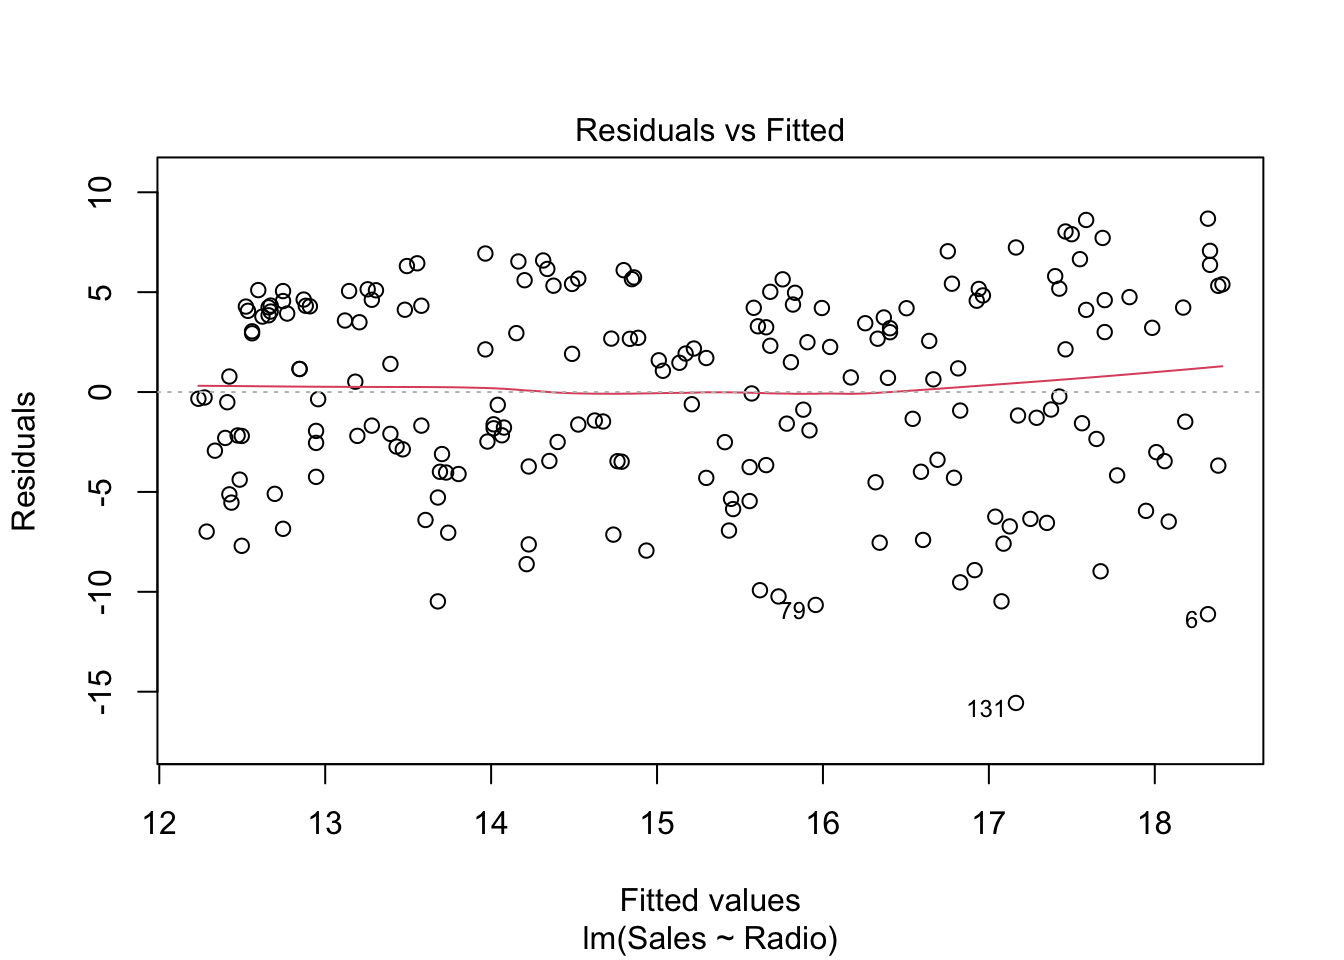
\includegraphics{smr_book_files/figure-latex/unnamed-chunk-125-1.pdf}

This shows how the residuals \(e\) are distributed against the
fitted values (or predictions) \(\hat{y}\). Ideally, there should
be no correlation, i.e.~randomly spread around 0. If that is not
the case and the plot shows a trend, the assumption of a linear
regression model might not be appropriate.

\begin{Shaded}
\begin{Highlighting}[]
\CommentTok{\# normal q{-}q plot}
\FunctionTok{plot}\NormalTok{(radio\_lm, }\AttributeTok{which =} \DecValTok{2}\NormalTok{)}
\end{Highlighting}
\end{Shaded}

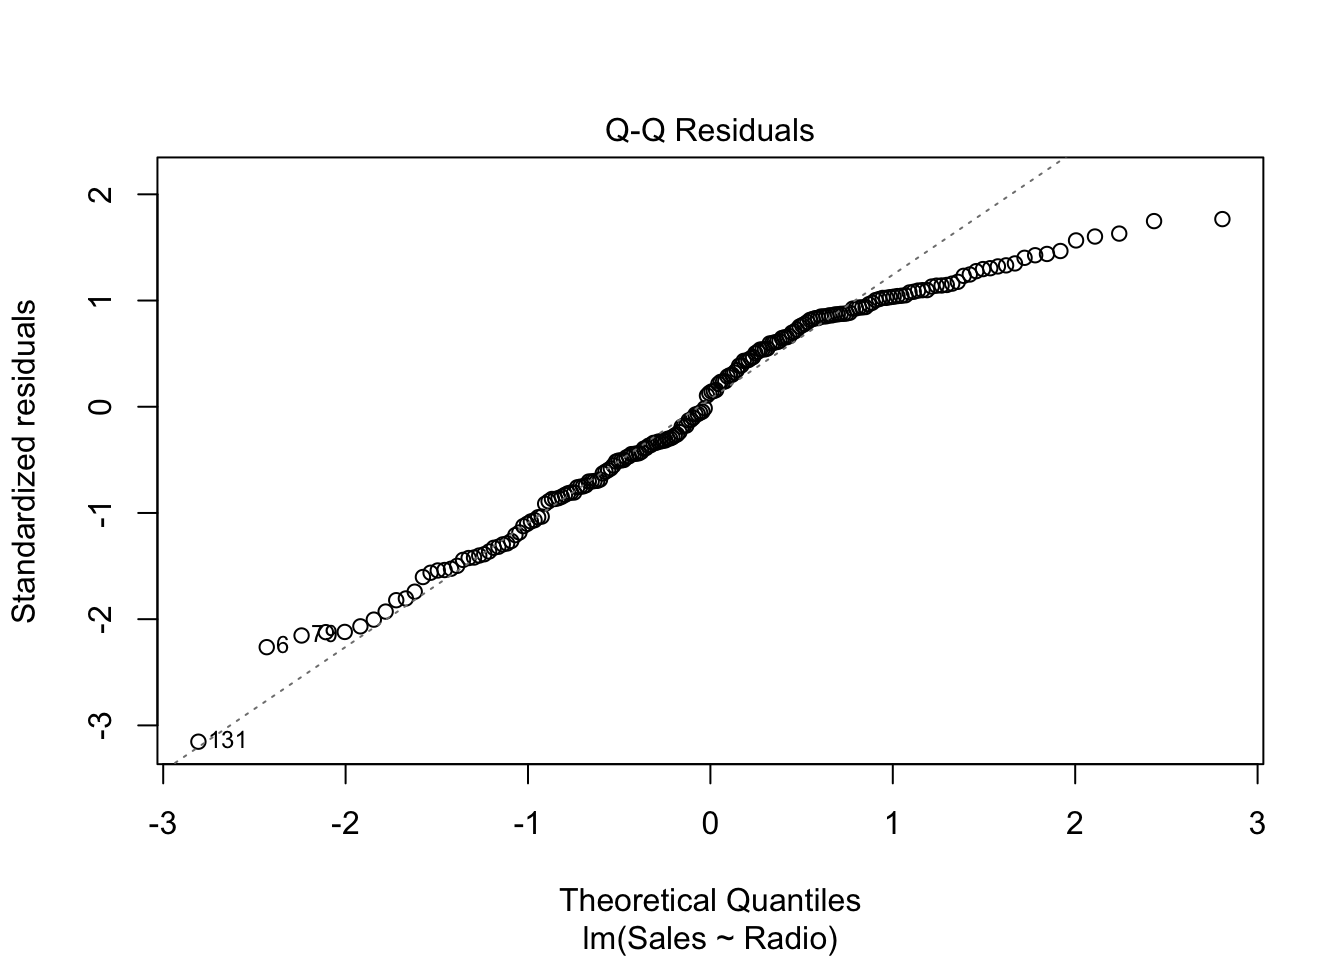
\includegraphics{smr_book_files/figure-latex/unnamed-chunk-126-1.pdf}

The Q-Q plot compares two distributions (or one theoretical distribution
with an empirical one). Given some data, the question it helps
answering to is: \emph{is one distribution close to the other one?}
In particular, the above plot is a Normal Q-Q plot of \(e\),
where its (standardized) distribution is compared to the standard
normal distribution.
More precisely, once the residuals are standardized (i.e.~minus the mean,
divided by the standard deviation) and sorted in ascending order, they are
plotted against the theoretical quantiles of the standard Normal distributions.
Example: the theoretical quantile of the \(k^{\text{th}}\) residual (in ascending
order) is \(q_{\alpha}\) where \(\alpha = P(Z <= q_{\alpha}) = k / n\)

Exercise: draw a Q-Q plot ``by hand'':

\begin{Shaded}
\begin{Highlighting}[]
\NormalTok{n }\OtherTok{\textless{}{-}} \FunctionTok{nrow}\NormalTok{(advertising)}
\NormalTok{std\_res }\OtherTok{\textless{}{-}} \FunctionTok{with}\NormalTok{(radio\_lm, \{}
  \FunctionTok{sort}\NormalTok{((residuals }\SpecialCharTok{{-}} \FunctionTok{mean}\NormalTok{(residuals)) }\SpecialCharTok{/} \FunctionTok{sd}\NormalTok{(residuals),}
    \AttributeTok{decreasing =} \ConstantTok{FALSE}
\NormalTok{  )}
\NormalTok{\})}
\NormalTok{th\_q }\OtherTok{\textless{}{-}} \FunctionTok{qnorm}\NormalTok{(}\DecValTok{1}\SpecialCharTok{:}\NormalTok{n }\SpecialCharTok{/}\NormalTok{ n)}
\FunctionTok{plot}\NormalTok{(th\_q, std\_res)}
\end{Highlighting}
\end{Shaded}

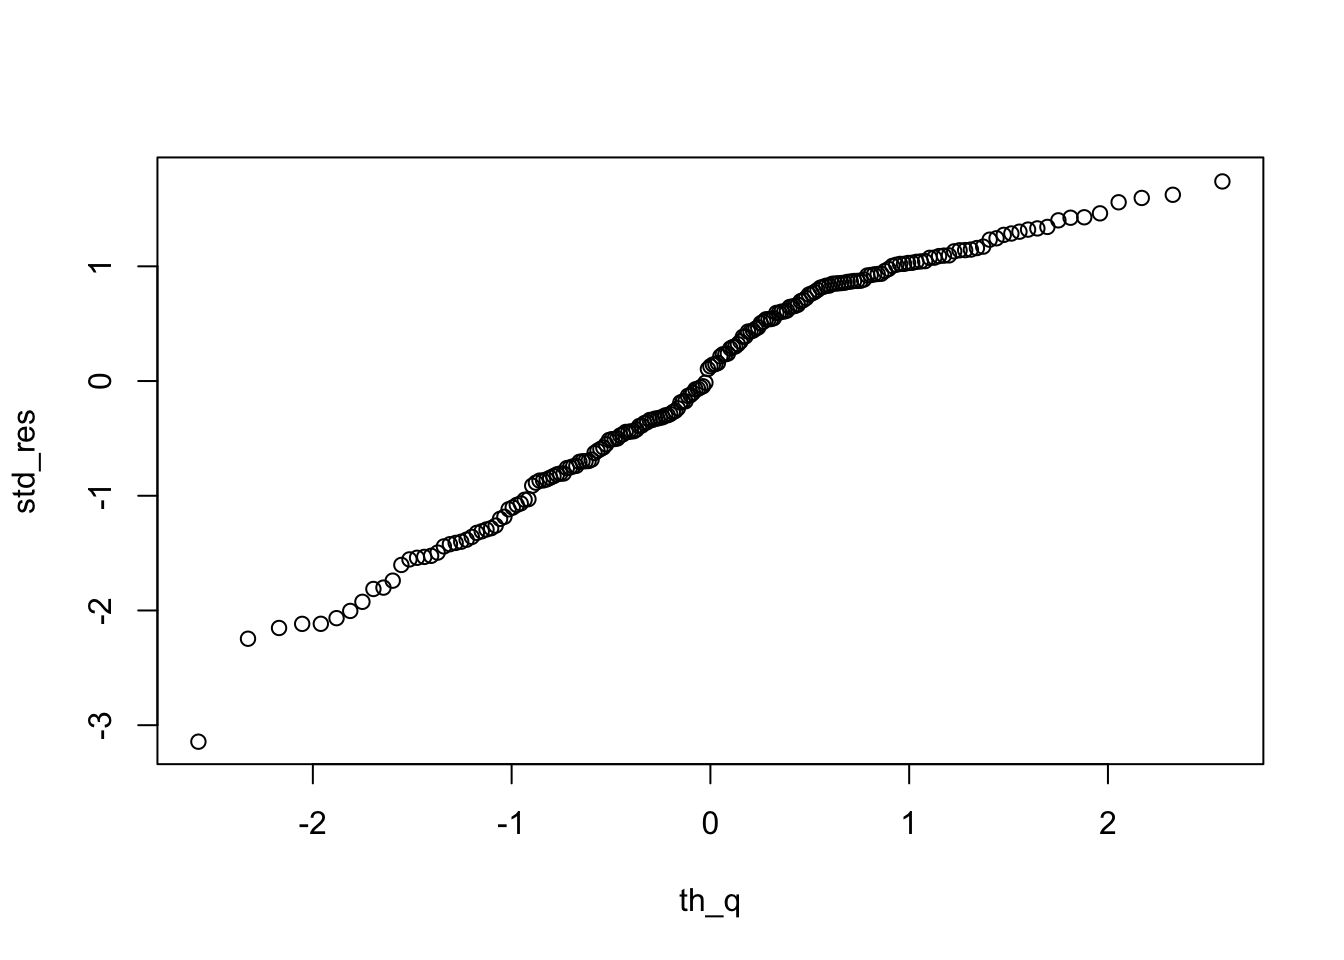
\includegraphics{smr_book_files/figure-latex/unnamed-chunk-127-1.pdf}

\begin{quote}
Note: the standardized residuals are actually computed slightly
differently by the \texttt{plot.lm} R function, but this standardization
is good enough for our purpose. Check the details in the help
document \texttt{?plot.lm}.
\end{quote}

\begin{Shaded}
\begin{Highlighting}[]
\CommentTok{\# scale{-}location}
\FunctionTok{plot}\NormalTok{(radio\_lm, }\AttributeTok{which =} \DecValTok{3}\NormalTok{)}
\end{Highlighting}
\end{Shaded}

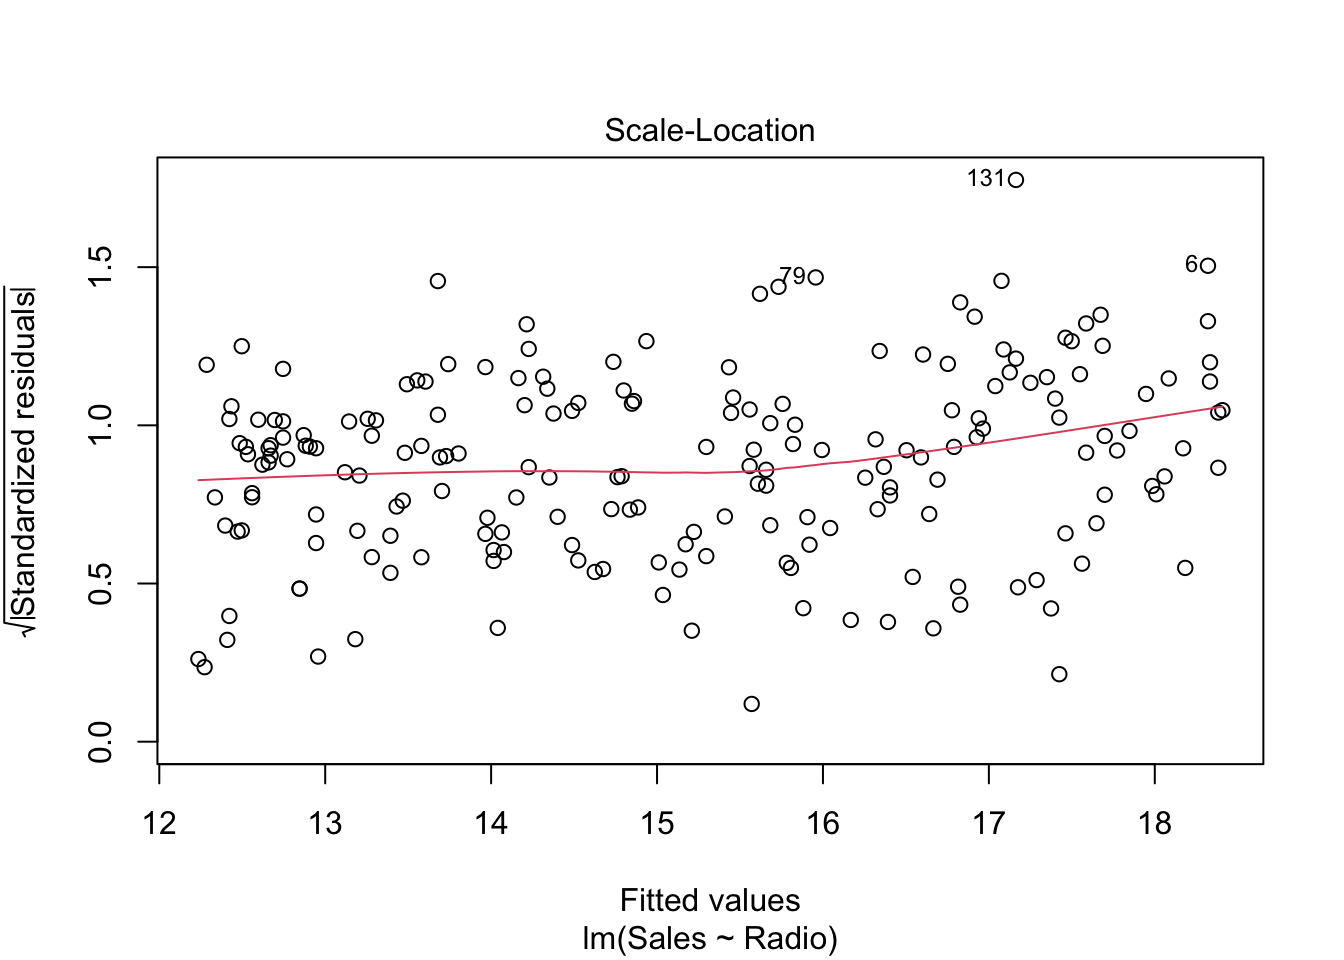
\includegraphics{smr_book_files/figure-latex/unnamed-chunk-128-1.pdf}

This plot only reduces the skewness of the standardized
residuals by taking its square root.

\begin{Shaded}
\begin{Highlighting}[]
\CommentTok{\# residuals vs leverage}
\FunctionTok{plot}\NormalTok{(radio\_lm, }\AttributeTok{which =} \DecValTok{5}\NormalTok{)}
\end{Highlighting}
\end{Shaded}

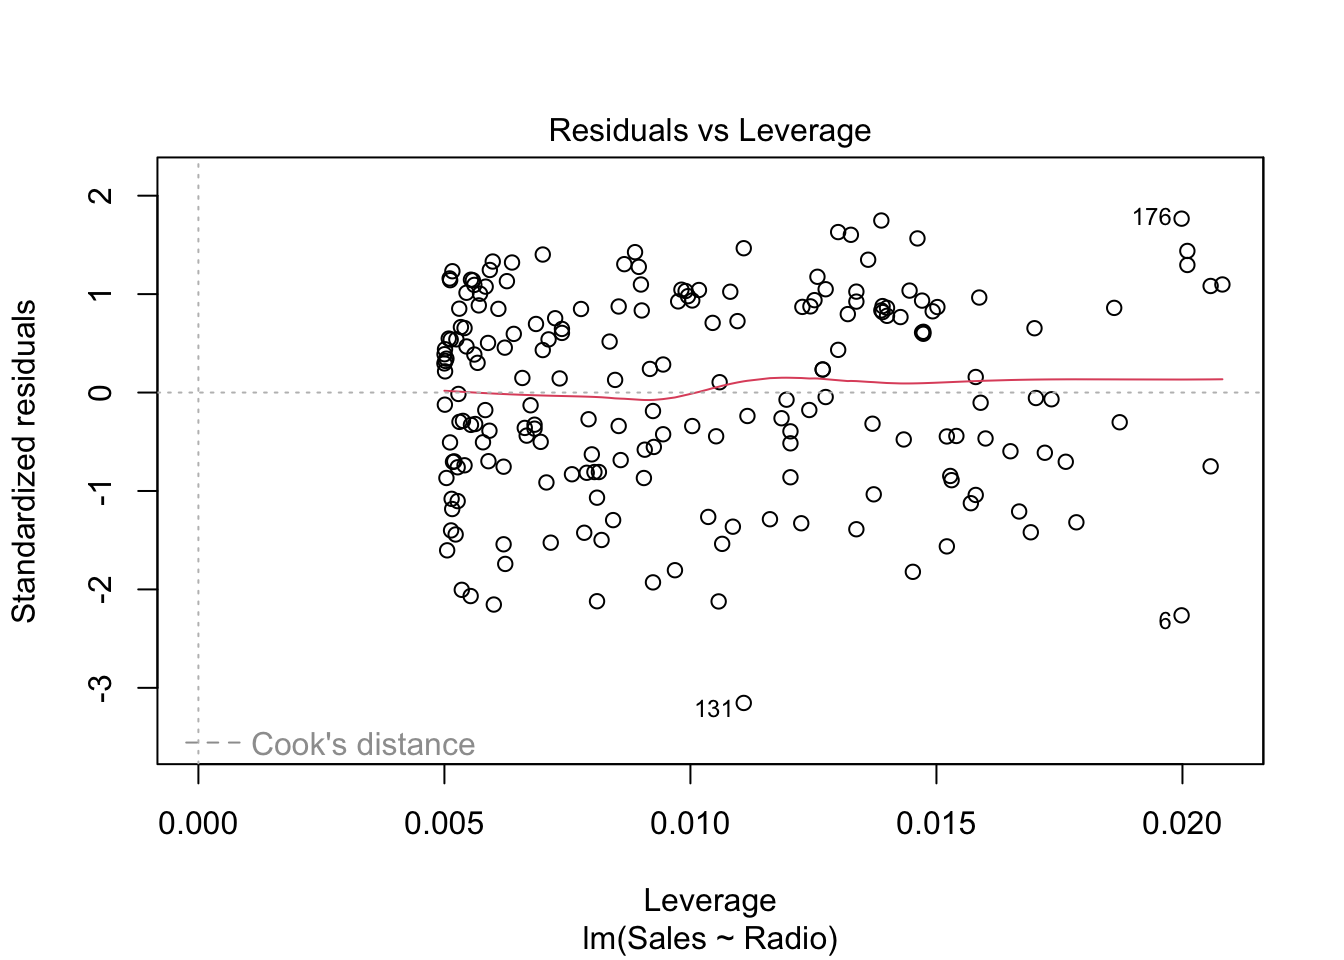
\includegraphics{smr_book_files/figure-latex/unnamed-chunk-129-1.pdf}
In order to understand this plot we have to introduced the
so-called \emph{hat matrix}

\[
H = X (X'X)^{-1} X'
\]

which is the projection matrix that maps \(Y\) to \(\hat Y\).
Its diagonal elements are particularly interesting and are called
leverages of the observations. Note that \(h_{ii} \in [0,1]\) and
\(\sum_i h_{ii} = p\), where \(p\) is the number of coefficients in the regression model.
The leverage of an observation \(h_{ii}\) measures how much an observation \(y_i\)
has an impact on the fitted value \(\hat y_i\).\footnote{Explanation taken from
  \url{https://it.mathworks.com/help/stats/hat-matrix-and-leverage.html}}

\section{Multiple predictors}\label{multiple-predictors}

Predictors in R linear models are defined in the formula.

\textbf{What is a formula?}

In R, \texttt{y\ \textasciitilde{}\ x\ +\ b} is a formula.

\begin{itemize}
\tightlist
\item
  \texttt{y} is the dependent variable(s) (e.g.~response, label)
\item
  \texttt{x\ +\ b} are the independent variables (e.g.~predictors/features)
\item
  can also be one-sided e.g.~\texttt{\textasciitilde{}\ x}
\item
  \texttt{+} (plus) sign is not a sum, but a \emph{join} operator
\item
  when formulae are written, variables are not evaluated (symbolic model)
\item
  you can exclude some terms explicitly by using \texttt{-} (e.g.~\texttt{y\ \textasciitilde{}\ x\ -\ 1}
  will only estimate the \texttt{x} coefficient and not the intercept, which
  is implicitly added by \texttt{lm})
\end{itemize}

More on formulae later (see Interactions in the next lesson).

\emph{Examples}:

\begin{Shaded}
\begin{Highlighting}[]
\NormalTok{f }\OtherTok{\textless{}{-}}\NormalTok{ y }\SpecialCharTok{\textasciitilde{}}\NormalTok{ x }\SpecialCharTok{+}\NormalTok{ b}
\FunctionTok{class}\NormalTok{(f)}
\end{Highlighting}
\end{Shaded}

\begin{verbatim}
## [1] "formula"
\end{verbatim}

\begin{Shaded}
\begin{Highlighting}[]
\NormalTok{f[[}\DecValTok{1}\NormalTok{]] }\CommentTok{\# formula symbol}
\end{Highlighting}
\end{Shaded}

\begin{verbatim}
## `~`
\end{verbatim}

\begin{Shaded}
\begin{Highlighting}[]
\NormalTok{f[[}\DecValTok{2}\NormalTok{]] }\CommentTok{\# dep vars}
\end{Highlighting}
\end{Shaded}

\begin{verbatim}
## y
\end{verbatim}

\begin{Shaded}
\begin{Highlighting}[]
\NormalTok{f[[}\DecValTok{3}\NormalTok{]] }\CommentTok{\# indep vars}
\end{Highlighting}
\end{Shaded}

\begin{verbatim}
## x + b
\end{verbatim}

Generally, a linear model formula is composed by multiple
predictors.

\begin{Shaded}
\begin{Highlighting}[]
\NormalTok{complete\_lm }\OtherTok{\textless{}{-}} \FunctionTok{lm}\NormalTok{(Sales }\SpecialCharTok{\textasciitilde{}}\NormalTok{ TV }\SpecialCharTok{+}\NormalTok{ Radio }\SpecialCharTok{+}\NormalTok{ Newspaper, }\AttributeTok{data =}\NormalTok{ advertising)}
\CommentTok{\# or}
\NormalTok{complete\_lm }\OtherTok{\textless{}{-}} \FunctionTok{lm}\NormalTok{(Sales }\SpecialCharTok{\textasciitilde{}}\NormalTok{ ., }\AttributeTok{data =}\NormalTok{ advertising)}
\end{Highlighting}
\end{Shaded}

The dot stands for all the possible predictors in the dataset.

\begin{Shaded}
\begin{Highlighting}[]
\FunctionTok{summary}\NormalTok{(complete\_lm)}
\end{Highlighting}
\end{Shaded}

\begin{verbatim}
## 
## Call:
## lm(formula = Sales ~ ., data = advertising)
## 
## Residuals:
##     Min      1Q  Median      3Q     Max 
## -7.3034 -0.8244 -0.0008  0.8976  3.7473 
## 
## Coefficients:
##              Estimate Std. Error t value Pr(>|t|)    
## (Intercept) 4.6251241  0.3075012  15.041   <2e-16 ***
## TV          0.0544458  0.0013752  39.592   <2e-16 ***
## Radio       0.1070012  0.0084896  12.604   <2e-16 ***
## Newspaper   0.0003357  0.0057881   0.058    0.954    
## ---
## Signif. codes:  0 '***' 0.001 '**' 0.01 '*' 0.05 '.' 0.1 ' ' 1
## 
## Residual standard error: 1.662 on 196 degrees of freedom
## Multiple R-squared:  0.9026, Adjusted R-squared:  0.9011 
## F-statistic: 605.4 on 3 and 196 DF,  p-value: < 2.2e-16
\end{verbatim}

\section{Confidence regions}\label{confidence-regions}

The hypothesis system setup (in the general case, multiple regression) is:

\[
\begin{aligned}
H_0: &\quad C \beta = \theta\\
H_1: &\quad C \beta \neq \theta
\end{aligned}
\]

The confidence region for \(\beta\) is given by the theorem by which:

\[
\frac{(C\beta - C\hat\beta)' (C(X'X)^{-1}C')^{-1}(C\beta - C\hat\beta)}
{q \text{MSR}} \sim F(q, n-p)
\]

where \(\text{rank}(C) = q \leq p\).

In case of \(C = I\), the \((1 - \alpha)\)-confidence region
is an ellipsoid in \(\mathbb{R}^p\).

\[
(\hat\beta - \beta) X' X (\hat\beta - \beta) \leq 
F_{\alpha}(p, n-p) p \text{MSR}
\]

As already seen before, some plotting functions also draw a confidence region
for the regression line.

\begin{Shaded}
\begin{Highlighting}[]
\FunctionTok{library}\NormalTok{(ggplot2)}
\FunctionTok{ggplot}\NormalTok{(radio\_lm, }\AttributeTok{mapping =} \FunctionTok{aes}\NormalTok{(Radio, Sales)) }\SpecialCharTok{+}
  \FunctionTok{geom\_point}\NormalTok{() }\SpecialCharTok{+}
  \FunctionTok{geom\_smooth}\NormalTok{(}\AttributeTok{method =} \StringTok{"lm"}\NormalTok{, }\AttributeTok{color =} \StringTok{"red"}\NormalTok{)}
\end{Highlighting}
\end{Shaded}

\begin{verbatim}
## `geom_smooth()` using formula = 'y ~ x'
\end{verbatim}

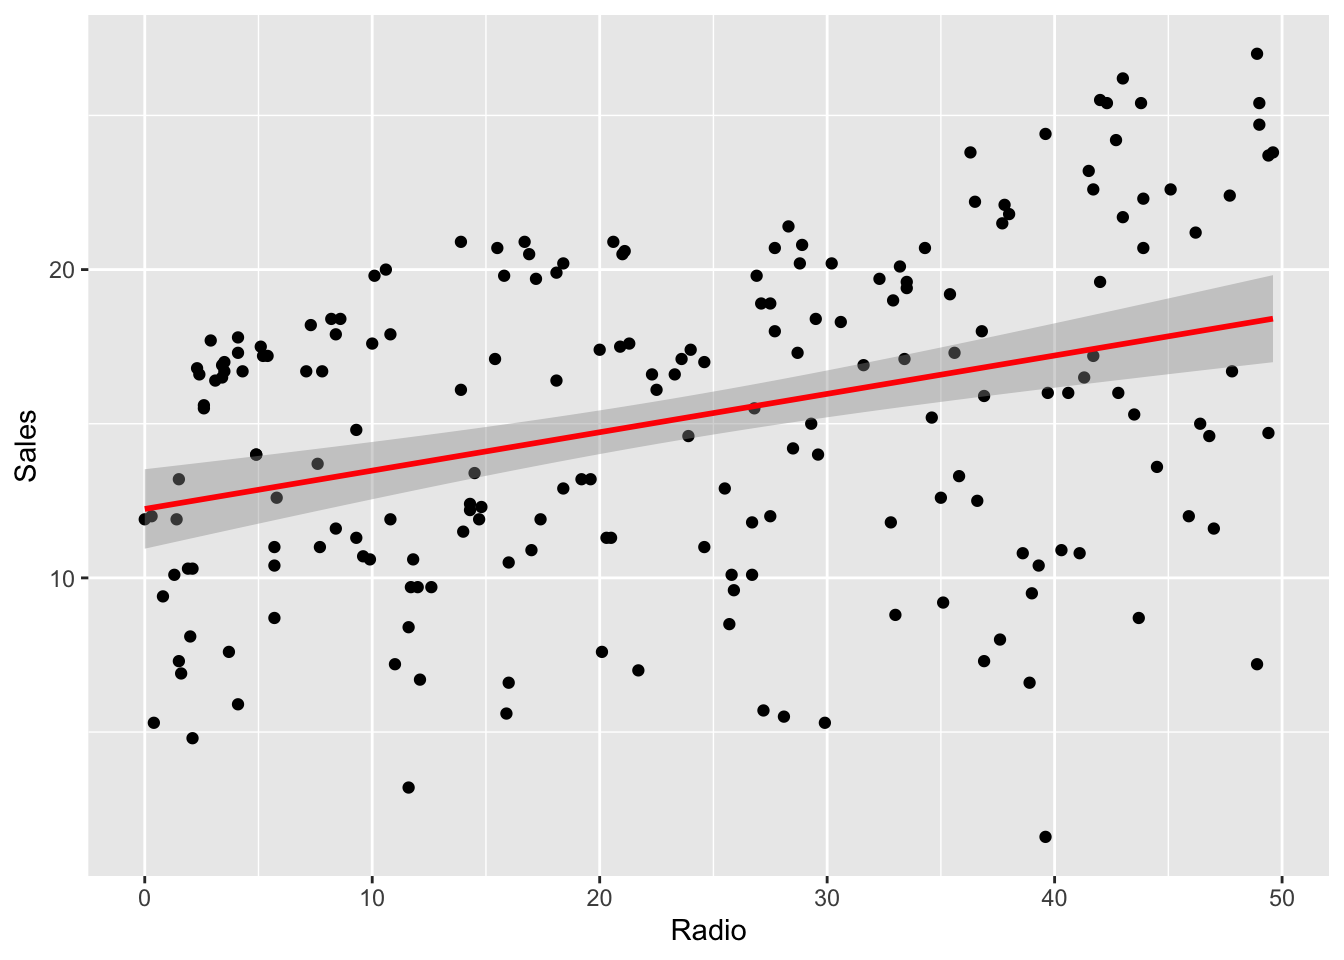
\includegraphics{smr_book_files/figure-latex/unnamed-chunk-133-1.pdf}

This confidence region is drawn according to that formula.

To get the confidence intervals values, just use \texttt{confint()}

\begin{Shaded}
\begin{Highlighting}[]
\FunctionTok{confint}\NormalTok{(radio\_lm)}
\end{Highlighting}
\end{Shaded}

\begin{verbatim}
##                   2.5 %     97.5 %
## (Intercept) 10.94703557 13.5244084
## Radio        0.07770266  0.1711606
\end{verbatim}

\begin{Shaded}
\begin{Highlighting}[]
\NormalTok{lb }\OtherTok{\textless{}{-}} \FunctionTok{confint}\NormalTok{(radio\_lm)[, }\DecValTok{1}\NormalTok{]}
\NormalTok{ub }\OtherTok{\textless{}{-}} \FunctionTok{confint}\NormalTok{(radio\_lm)[, }\DecValTok{2}\NormalTok{]}
\end{Highlighting}
\end{Shaded}

To plot it, e.g.~using \texttt{ggplot}:

\begin{Shaded}
\begin{Highlighting}[]
\CommentTok{\# prevision region}
\FunctionTok{ggplot}\NormalTok{(radio\_lm) }\SpecialCharTok{+}
  \FunctionTok{geom\_point}\NormalTok{(}\AttributeTok{mapping =} \FunctionTok{aes}\NormalTok{(Radio, Sales)) }\SpecialCharTok{+}
  \FunctionTok{geom\_abline}\NormalTok{(}
    \AttributeTok{intercept =}\NormalTok{ radio\_lm}\SpecialCharTok{$}\NormalTok{coefficients[[}\DecValTok{1}\NormalTok{]],}
    \AttributeTok{slope =}\NormalTok{ radio\_lm}\SpecialCharTok{$}\NormalTok{coefficients[[}\DecValTok{2}\NormalTok{]], }\AttributeTok{color =} \DecValTok{1}
\NormalTok{  ) }\SpecialCharTok{+}
  \FunctionTok{geom\_abline}\NormalTok{(}\AttributeTok{intercept =}\NormalTok{ lb[}\DecValTok{1}\NormalTok{], }\AttributeTok{slope =}\NormalTok{ lb[}\DecValTok{2}\NormalTok{], }\AttributeTok{color =} \DecValTok{2}\NormalTok{) }\SpecialCharTok{+}
  \FunctionTok{geom\_abline}\NormalTok{(}\AttributeTok{intercept =}\NormalTok{ ub[}\DecValTok{1}\NormalTok{], }\AttributeTok{slope =}\NormalTok{ ub[}\DecValTok{2}\NormalTok{], }\AttributeTok{color =} \DecValTok{2}\NormalTok{)}
\end{Highlighting}
\end{Shaded}

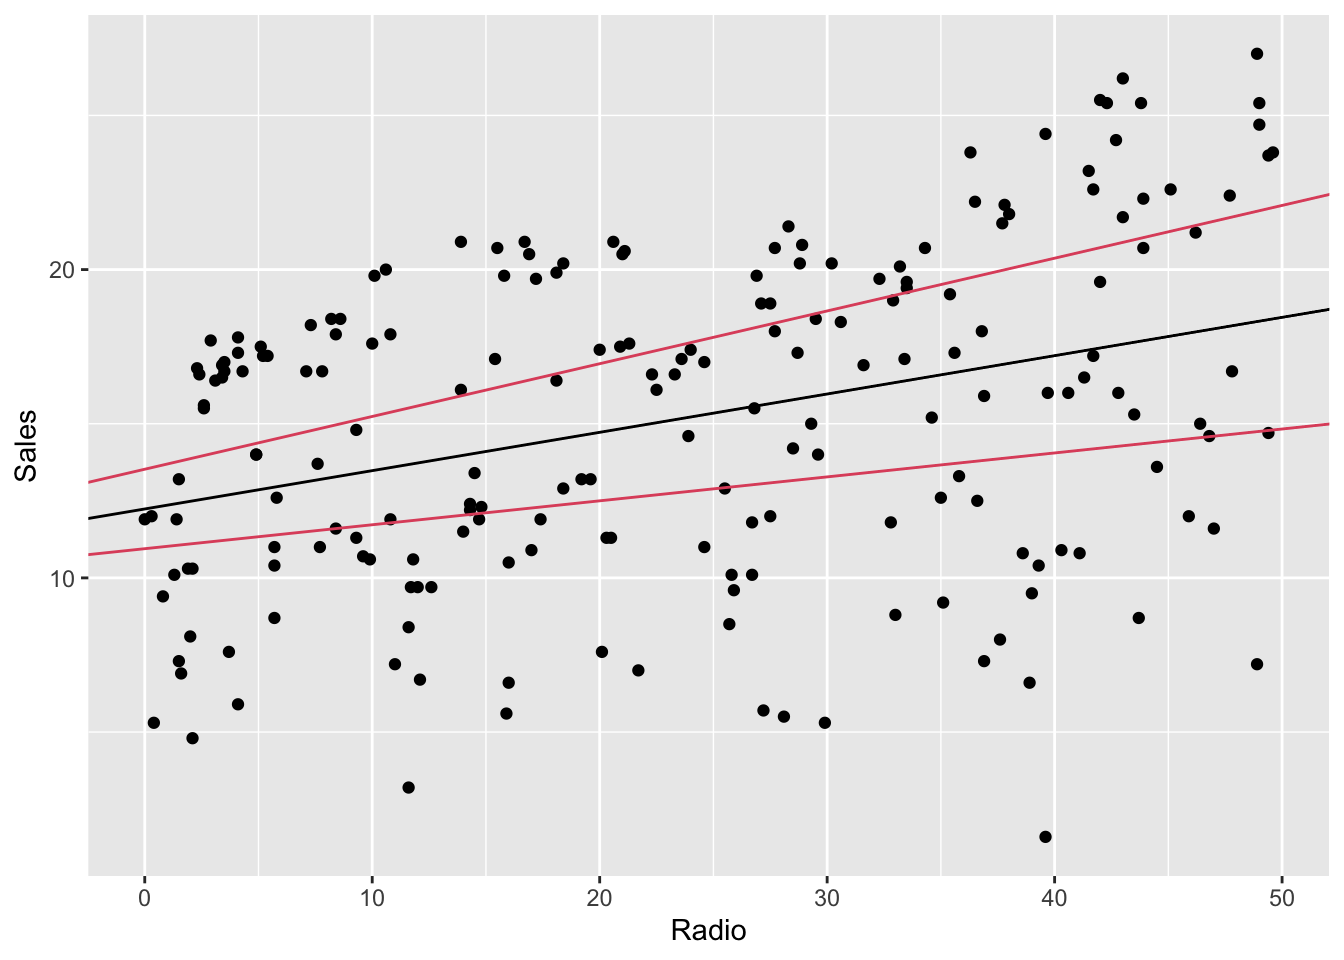
\includegraphics{smr_book_files/figure-latex/unnamed-chunk-135-1.pdf}

The region between the lines is different (larger) from the one generated by
\texttt{geom\_smooth}. Without entering too much in detail, this happens because the
confidence intervals in the second case are computed independently one
coefficients from the other, while in ggplot's function the confidence region
is jointly computed, therefore it's more accurate.

\chapter{Interactions and qualitative predictors}\label{interactions-and-qualitative-predictors}

\section{Transformations}\label{transformations}

Formulae in R linear models are much more powerful than
what seen so far. In some cases we might be interested in
transforming a variable before fitting the linear model.

\subsection{A simple example}\label{a-simple-example}

For instance, let's take this synthetic dataset:

\begin{Shaded}
\begin{Highlighting}[]
\FunctionTok{library}\NormalTok{(tibble)}
\NormalTok{n }\OtherTok{\textless{}{-}} \DecValTok{100}
\NormalTok{synth }\OtherTok{\textless{}{-}} \FunctionTok{tibble}\NormalTok{(}
  \AttributeTok{x =} \FunctionTok{seq}\NormalTok{(}\AttributeTok{from =} \DecValTok{1}\NormalTok{, }\AttributeTok{to =} \DecValTok{30}\NormalTok{, }\AttributeTok{length.out =}\NormalTok{ n),}
  \AttributeTok{y =} \FunctionTok{log}\NormalTok{(x) }\SpecialCharTok{+} \FunctionTok{rnorm}\NormalTok{(n, }\DecValTok{0}\NormalTok{, }\FloatTok{0.2}\NormalTok{)}
\NormalTok{)}
\end{Highlighting}
\end{Shaded}

which looks like this:

\begin{Shaded}
\begin{Highlighting}[]
\FunctionTok{library}\NormalTok{(ggplot2)}
\FunctionTok{ggplot}\NormalTok{(synth) }\SpecialCharTok{+}
  \FunctionTok{geom\_point}\NormalTok{(}\FunctionTok{aes}\NormalTok{(x, y))}
\end{Highlighting}
\end{Shaded}

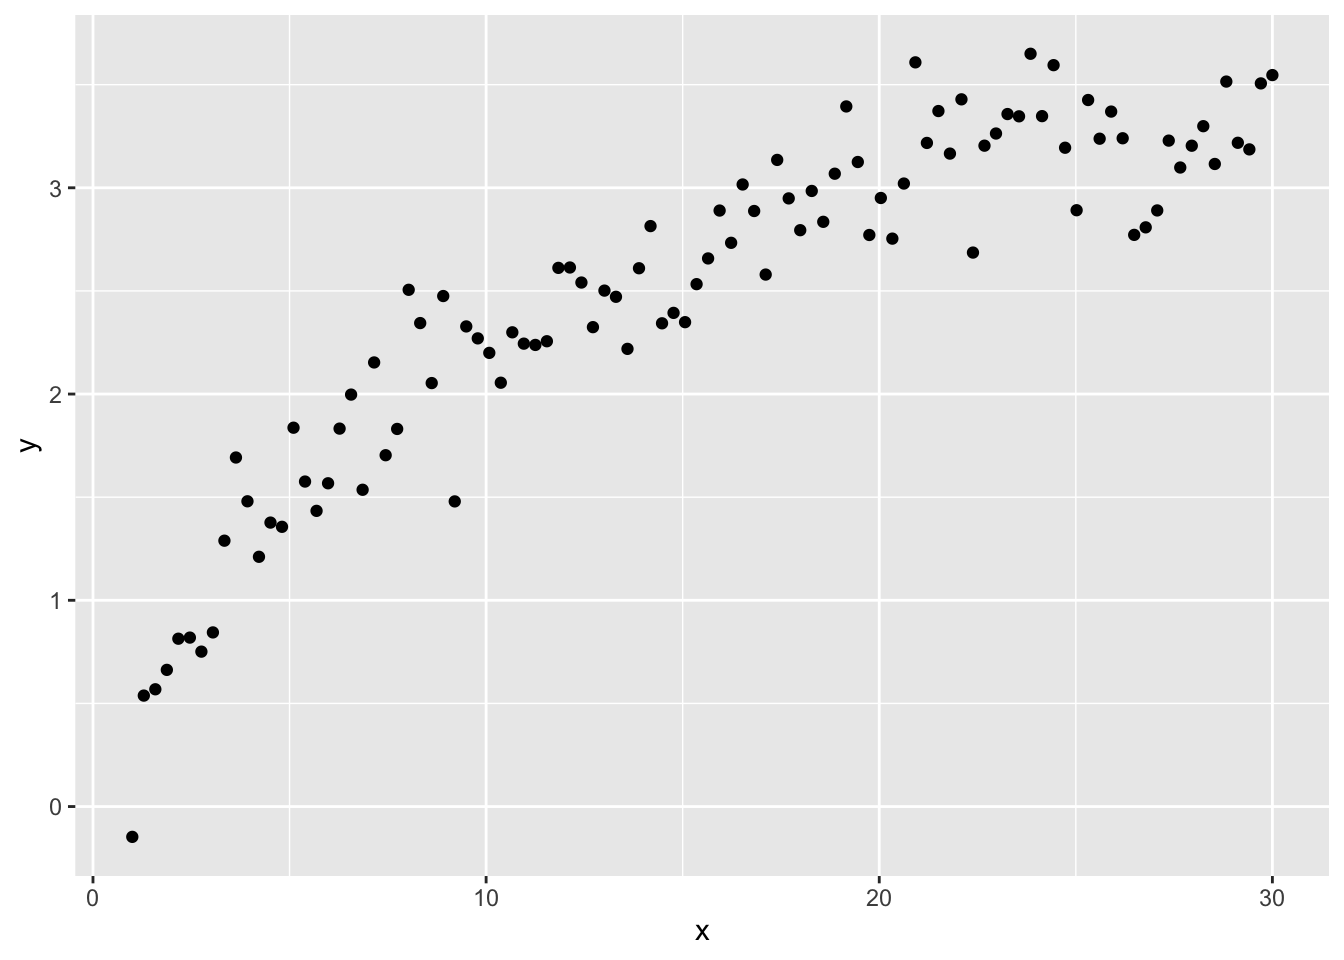
\includegraphics{smr_book_files/figure-latex/unnamed-chunk-138-1.pdf}

Of course, we can try to fit a linear model without any
extra effort

\begin{Shaded}
\begin{Highlighting}[]
\NormalTok{naive\_lm }\OtherTok{\textless{}{-}} \FunctionTok{lm}\NormalTok{(y }\SpecialCharTok{\textasciitilde{}}\NormalTok{ x, }\AttributeTok{data =}\NormalTok{ synth)}
\FunctionTok{ggplot}\NormalTok{(naive\_lm, }\AttributeTok{mapping =} \FunctionTok{aes}\NormalTok{(x, y)) }\SpecialCharTok{+}
  \FunctionTok{geom\_point}\NormalTok{() }\SpecialCharTok{+}
  \FunctionTok{geom\_smooth}\NormalTok{(}\AttributeTok{method =} \StringTok{"lm"}\NormalTok{, }\AttributeTok{color =} \StringTok{"red"}\NormalTok{)}
\end{Highlighting}
\end{Shaded}

\begin{verbatim}
## `geom_smooth()` using formula = 'y ~ x'
\end{verbatim}

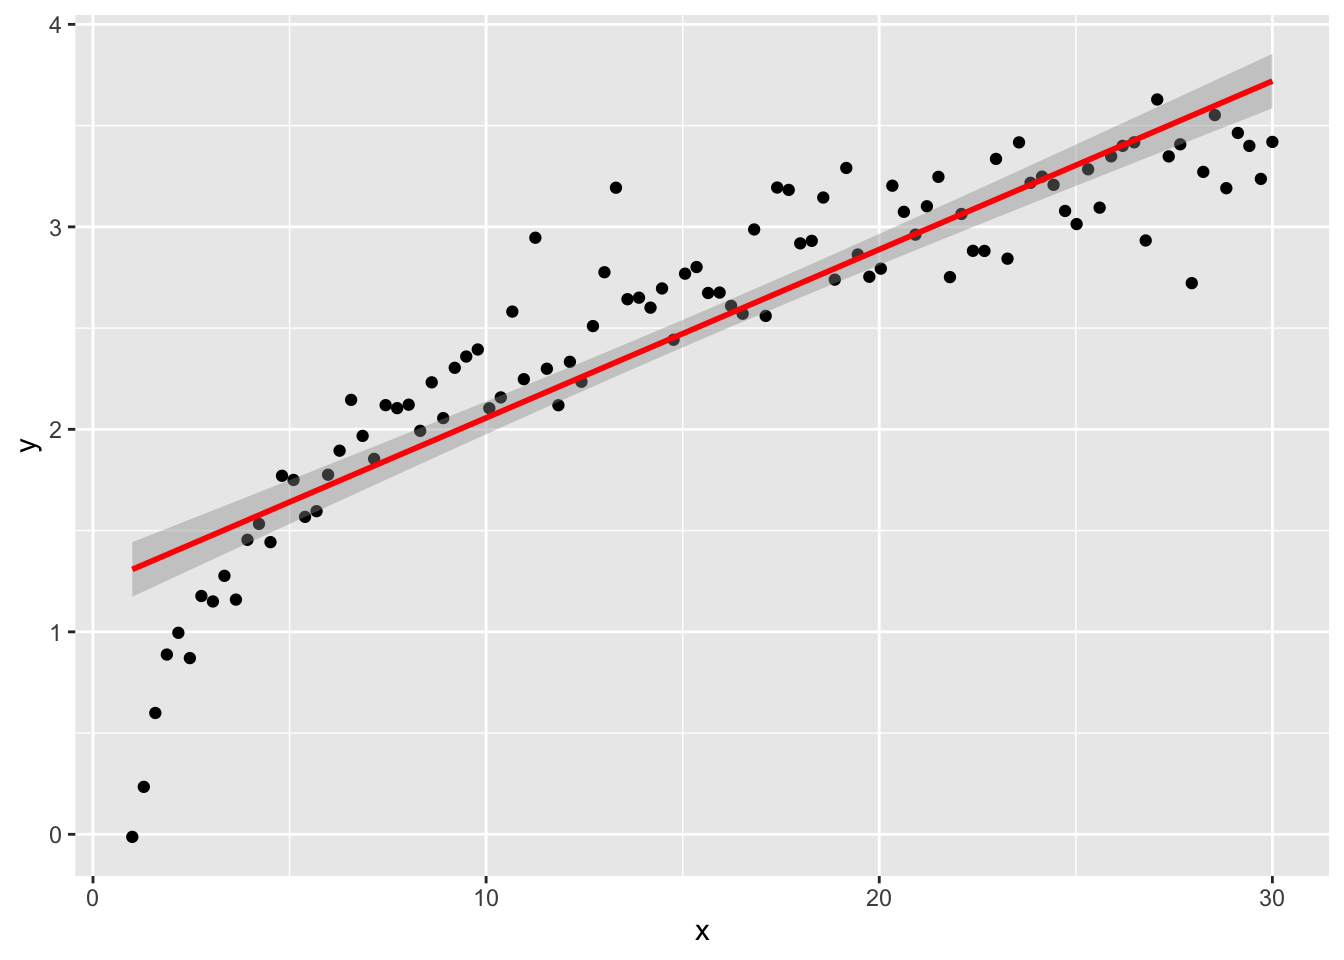
\includegraphics{smr_book_files/figure-latex/unnamed-chunk-139-1.pdf}

but if we plot the residuals, we can detect some issues for low
values of \(y\) (definitely not uncorrelated).

\begin{Shaded}
\begin{Highlighting}[]
\FunctionTok{library}\NormalTok{(dplyr)}
\NormalTok{synth }\SpecialCharTok{\%\textgreater{}\%}
  \FunctionTok{mutate}\NormalTok{(}\AttributeTok{res =}\NormalTok{ naive\_lm}\SpecialCharTok{$}\NormalTok{residuals) }\SpecialCharTok{\%\textgreater{}\%} \CommentTok{\# adds the residual column}
  \FunctionTok{ggplot}\NormalTok{() }\SpecialCharTok{+}
  \FunctionTok{geom\_point}\NormalTok{(}\FunctionTok{aes}\NormalTok{(y, res))}
\end{Highlighting}
\end{Shaded}

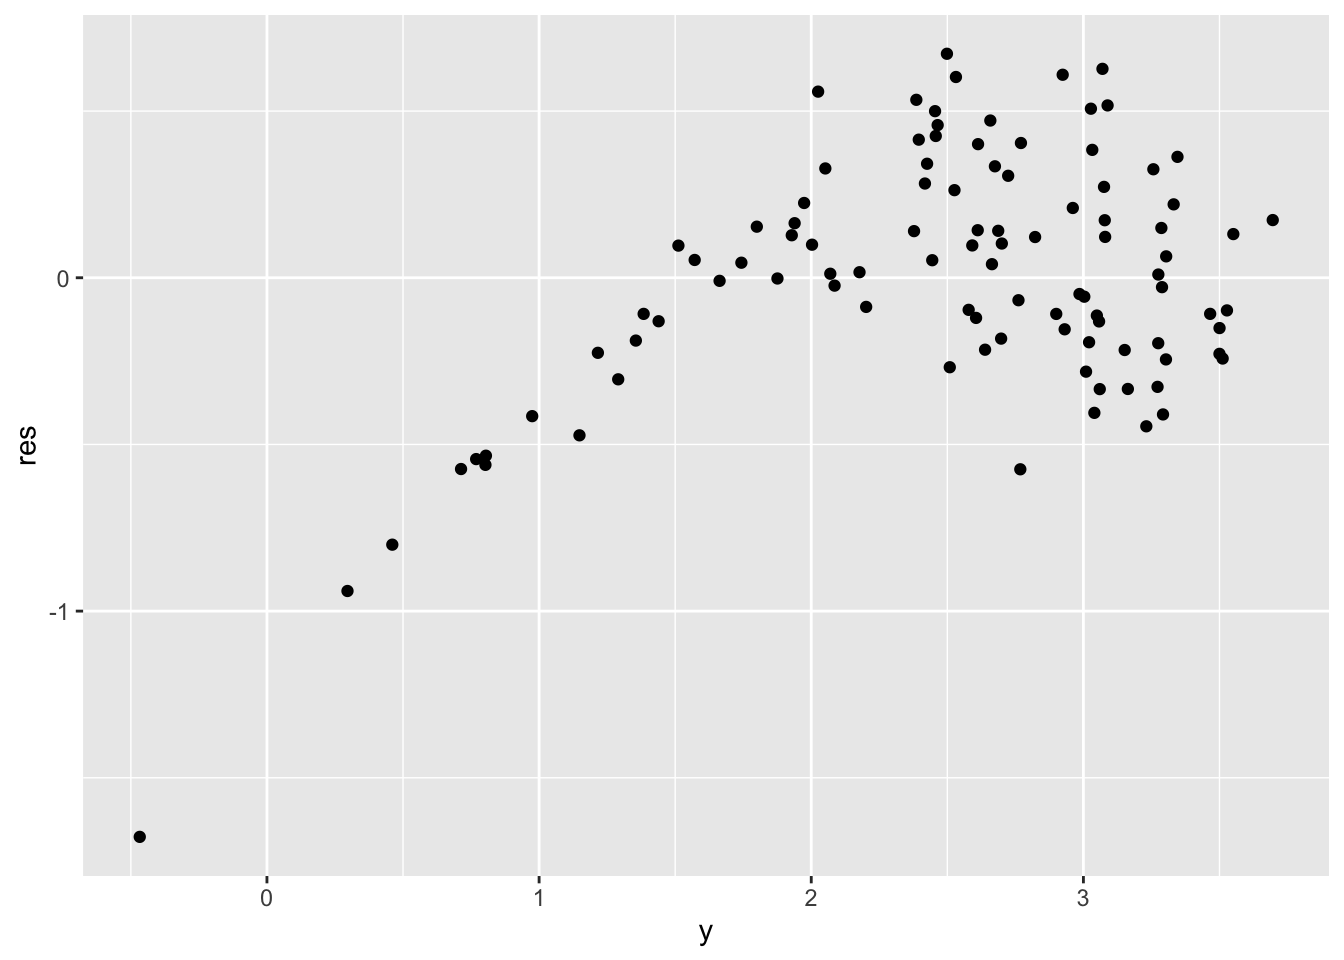
\includegraphics{smr_book_files/figure-latex/unnamed-chunk-140-1.pdf}

By understanding how \(x\) is distributed, we can fix this issue
and fit the model on a transformation of itself, clearly \(\log(x)\).
We do this simply by adding the desired transformation in the
formula, meaning that we don't have to tranform the dataset beforehand.

\begin{Shaded}
\begin{Highlighting}[]
\NormalTok{log\_lm }\OtherTok{\textless{}{-}} \FunctionTok{lm}\NormalTok{(y }\SpecialCharTok{\textasciitilde{}} \FunctionTok{log}\NormalTok{(x), }\AttributeTok{data =}\NormalTok{ synth)}
\FunctionTok{ggplot}\NormalTok{(log\_lm,}
  \AttributeTok{mapping =} \FunctionTok{aes}\NormalTok{(}\StringTok{\textasciigrave{}}\AttributeTok{log(x)}\StringTok{\textasciigrave{}}\NormalTok{, y)}
\NormalTok{) }\SpecialCharTok{+} \CommentTok{\# notice the backticks!}
  \FunctionTok{geom\_point}\NormalTok{() }\SpecialCharTok{+}
  \FunctionTok{geom\_smooth}\NormalTok{(}\AttributeTok{method =} \StringTok{"lm"}\NormalTok{, }\AttributeTok{color =} \StringTok{"red"}\NormalTok{)}
\end{Highlighting}
\end{Shaded}

\begin{verbatim}
## `geom_smooth()` using formula = 'y ~ x'
\end{verbatim}

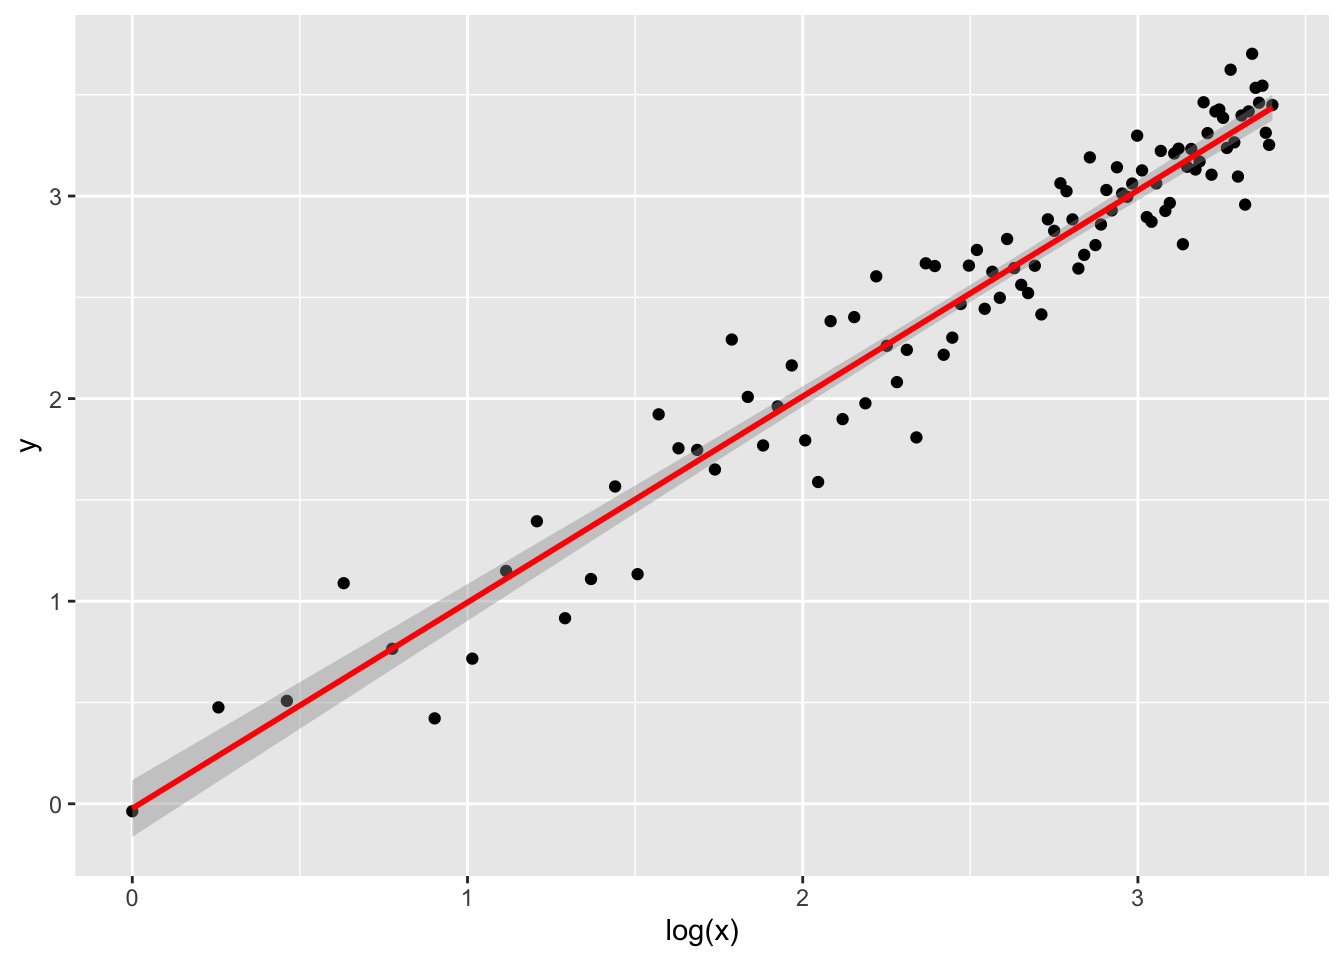
\includegraphics{smr_book_files/figure-latex/unnamed-chunk-141-1.pdf}

and the residuals plot.

\begin{Shaded}
\begin{Highlighting}[]
\NormalTok{synth }\SpecialCharTok{\%\textgreater{}\%}
  \FunctionTok{mutate}\NormalTok{(}\AttributeTok{res =}\NormalTok{ log\_lm}\SpecialCharTok{$}\NormalTok{residuals) }\SpecialCharTok{\%\textgreater{}\%} \CommentTok{\# adds the residual column}
  \FunctionTok{ggplot}\NormalTok{() }\SpecialCharTok{+}
  \FunctionTok{geom\_point}\NormalTok{(}\FunctionTok{aes}\NormalTok{(y, res))}
\end{Highlighting}
\end{Shaded}

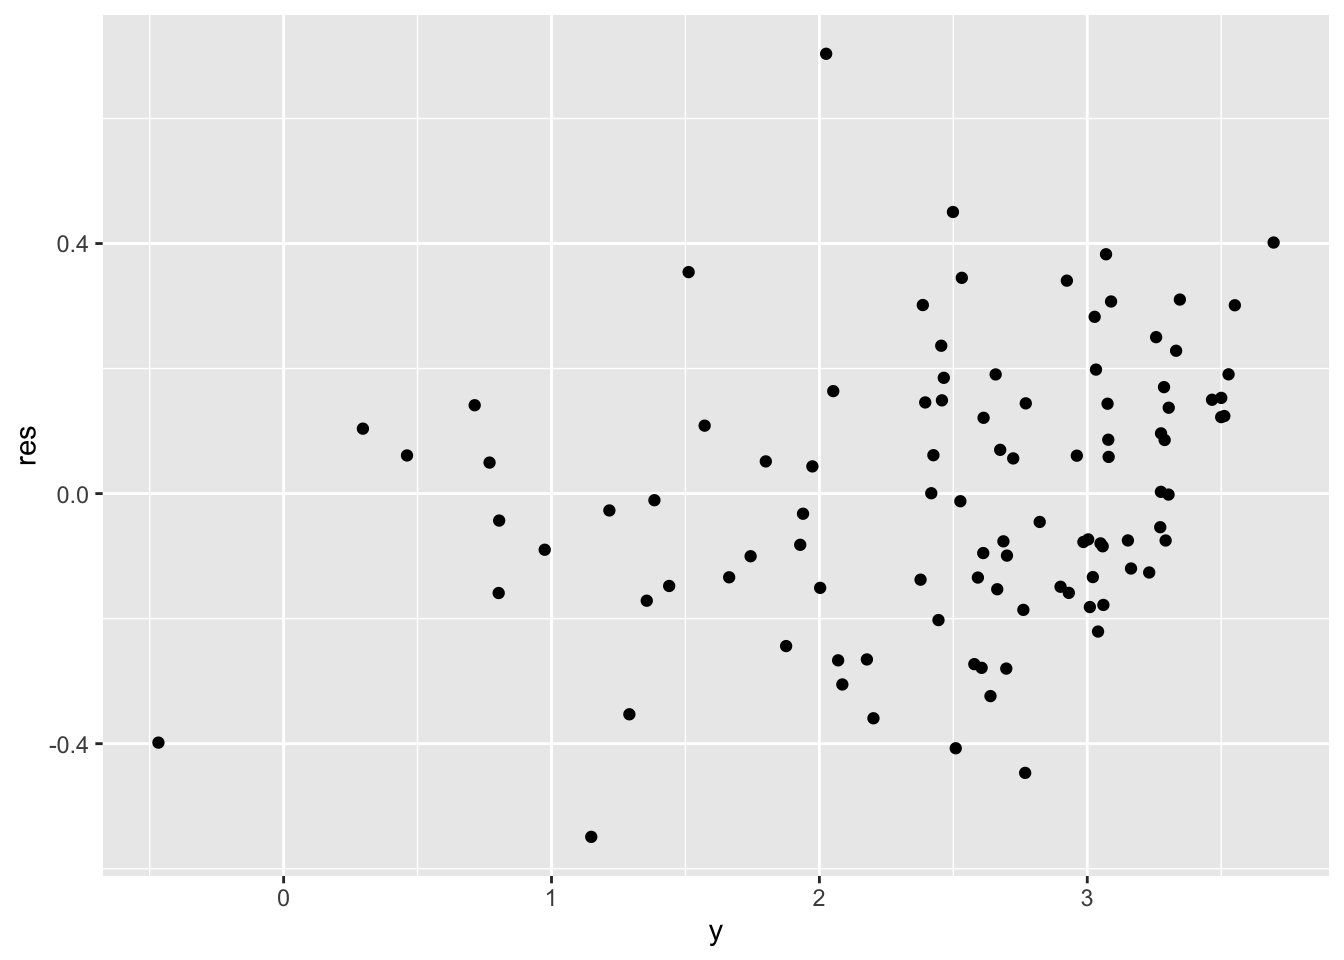
\includegraphics{smr_book_files/figure-latex/unnamed-chunk-142-1.pdf}

\subsection{\texorpdfstring{On \emph{advertising}}{On advertising}}\label{on-advertising}

Back to our real dataset.

\begin{Shaded}
\begin{Highlighting}[]
\FunctionTok{library}\NormalTok{(readr)}
\NormalTok{advertising }\OtherTok{\textless{}{-}} \FunctionTok{read\_csv}\NormalTok{(}\StringTok{"./datasets/advertising.csv"}\NormalTok{)}
\end{Highlighting}
\end{Shaded}

\begin{verbatim}
## Rows: 200 Columns: 4
## -- Column specification --------------------------------------------------------
## Delimiter: ","
## dbl (4): TV, Radio, Newspaper, Sales
## 
## i Use `spec()` to retrieve the full column specification for this data.
## i Specify the column types or set `show_col_types = FALSE` to quiet this message.
\end{verbatim}

Let's try applying a transformation to the most promising
predictor, in particular let's us \(\sqrt{TV}\). The choice
of the square root transformation comes from a first look
at the scatter plot shown previously (TV against Sales),
where we can detect a slightly curved trend which resembles
a curve \(y = \sqrt{x}\).

Let's plot the data after the transformation and observe
that its trend better fit a straight line.

\begin{Shaded}
\begin{Highlighting}[]
\NormalTok{advertising }\SpecialCharTok{\%\textgreater{}\%}
\NormalTok{  dplyr}\SpecialCharTok{::}\FunctionTok{select}\NormalTok{(Sales, TV) }\SpecialCharTok{\%\textgreater{}\%}
\NormalTok{  dplyr}\SpecialCharTok{::}\FunctionTok{mutate}\NormalTok{(}\AttributeTok{sqrtTV =} \FunctionTok{sqrt}\NormalTok{(TV)) }\SpecialCharTok{\%\textgreater{}\%}
  \FunctionTok{ggplot}\NormalTok{(}\FunctionTok{aes}\NormalTok{(sqrtTV, Sales)) }\SpecialCharTok{+}
  \FunctionTok{geom\_point}\NormalTok{() }\SpecialCharTok{+}
  \FunctionTok{geom\_smooth}\NormalTok{(}\AttributeTok{method =} \StringTok{"lm"}\NormalTok{, }\AttributeTok{color =} \StringTok{"red"}\NormalTok{)}
\end{Highlighting}
\end{Shaded}

\begin{verbatim}
## `geom_smooth()` using formula = 'y ~ x'
\end{verbatim}

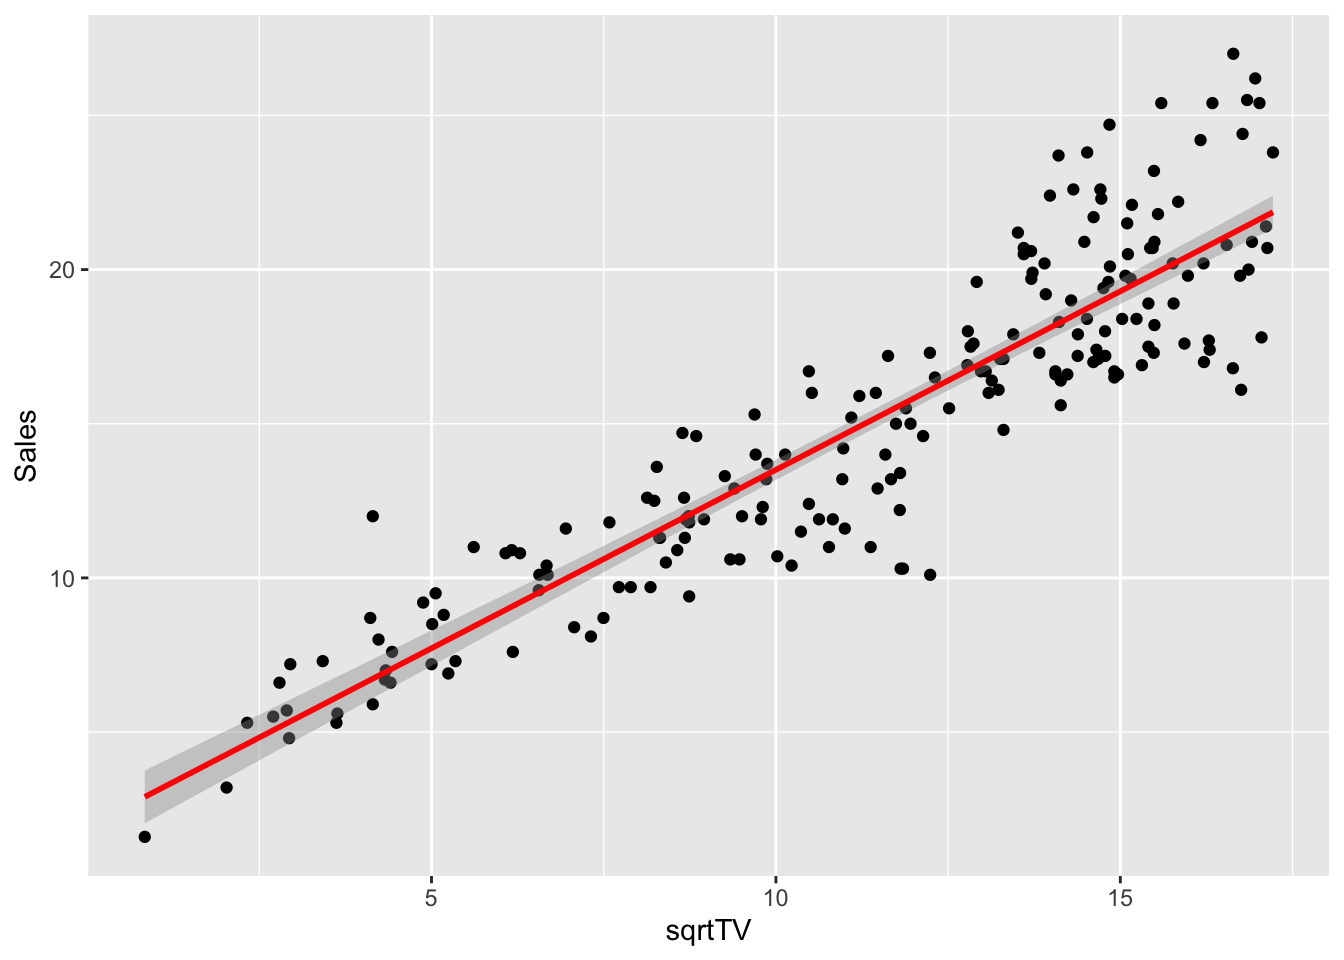
\includegraphics{smr_book_files/figure-latex/unnamed-chunk-144-1.pdf}

We can fit a linear model. Its \texttt{summary} table
will show a better \(R^2\) score.

\begin{Shaded}
\begin{Highlighting}[]
\NormalTok{trans\_lm }\OtherTok{\textless{}{-}} \FunctionTok{lm}\NormalTok{(Sales }\SpecialCharTok{\textasciitilde{}} \FunctionTok{sqrt}\NormalTok{(TV), }\AttributeTok{data =}\NormalTok{ advertising)}
\end{Highlighting}
\end{Shaded}

\begin{quote}
\emph{Exercise}: plot the regression line and compare it with
the simple model fitted on the raw data
\end{quote}

The following two commands might help in inspecting
a linear model with transformed data.

\begin{Shaded}
\begin{Highlighting}[]
\FunctionTok{head}\NormalTok{(}\FunctionTok{model.matrix}\NormalTok{(trans\_lm)) }\CommentTok{\# prints the design matrix}
\end{Highlighting}
\end{Shaded}

\begin{verbatim}
##   (Intercept)  sqrt(TV)
## 1           1 15.169047
## 2           1  6.670832
## 3           1  4.147288
## 4           1 12.308534
## 5           1 13.446189
## 6           1  2.949576
\end{verbatim}

\begin{Shaded}
\begin{Highlighting}[]
\NormalTok{trans\_lm}\SpecialCharTok{$}\NormalTok{terms }\CommentTok{\# inspect the linear model specifics}
\end{Highlighting}
\end{Shaded}

\begin{verbatim}
## Sales ~ sqrt(TV)
## attr(,"variables")
## list(Sales, sqrt(TV))
## attr(,"factors")
##          sqrt(TV)
## Sales           0
## sqrt(TV)        1
## attr(,"term.labels")
## [1] "sqrt(TV)"
## attr(,"order")
## [1] 1
## attr(,"intercept")
## [1] 1
## attr(,"response")
## [1] 1
## attr(,".Environment")
## <environment: R_GlobalEnv>
## attr(,"predvars")
## list(Sales, sqrt(TV))
## attr(,"dataClasses")
##     Sales  sqrt(TV) 
## "numeric" "numeric"
\end{verbatim}

\section{Model selection}\label{model-selection}

\subsection{R-squared}\label{r-squared}

One of the indicators computed with \texttt{summary} on a fitted linear model
is the \(R^2\) index (R-squared, or coefficient of determination). It is defined as

\[
R^2 = 1 - \frac{\sum_i (y_i - \hat y_i)^2}{\sum_i (y_i - \bar y)^2}
\]

and shows the impact of the residuals proportionately to the variance
of the response variable. It can be used to compare different models
although it should not be considered as an absolute score of the model.
The closer it is to 1, the better is the model fit.

This output, for instance, shows how the transformation used above
seems to improve the accuracy of the regression task.

\begin{Shaded}
\begin{Highlighting}[]
\NormalTok{simple\_lm }\OtherTok{\textless{}{-}} \FunctionTok{lm}\NormalTok{(Sales }\SpecialCharTok{\textasciitilde{}}\NormalTok{ TV, }\AttributeTok{data =}\NormalTok{ advertising)}
\FunctionTok{summary}\NormalTok{(simple\_lm)}\SpecialCharTok{$}\NormalTok{r.squared}
\end{Highlighting}
\end{Shaded}

\begin{verbatim}
## [1] 0.8121757
\end{verbatim}

\begin{Shaded}
\begin{Highlighting}[]
\FunctionTok{summary}\NormalTok{(trans\_lm)}\SpecialCharTok{$}\NormalTok{r.squared}
\end{Highlighting}
\end{Shaded}

\begin{verbatim}
## [1] 0.8216696
\end{verbatim}

\subsection{ANOVA}\label{anova}

Another way of comparing two models, in particular one model with
a smaller \emph{nested} model, is the ANOVA test, which is an instance
of the F-test, with statistics

\[
F = \frac{\left(\frac{RSS_1 - RSS_2}{p_2 - p_1}\right)}{\left(\frac{RSS_2}{n - p_2}\right)}
\]

where \(RSS\) is the residual sum of squares and \(p_2 > p_1\) (model 1 is
smaller). We know from theory that \(F \sim F(p_2 - p_1, n - p_2)\)

A low p-value for the F statistic means that we can reject the hypothesis that
the smaller model explains the data well enough.

Here we compare the model with a single predictor (squared root of TV), which
is the \emph{smaller} model, with a model with also the Radio data as
additional predictor.

\begin{Shaded}
\begin{Highlighting}[]
\NormalTok{double\_lm }\OtherTok{\textless{}{-}} \FunctionTok{lm}\NormalTok{(Sales }\SpecialCharTok{\textasciitilde{}} \FunctionTok{sqrt}\NormalTok{(TV) }\SpecialCharTok{+}\NormalTok{ Radio, }\AttributeTok{data =}\NormalTok{ advertising)}
\FunctionTok{anova}\NormalTok{(trans\_lm, double\_lm)}
\end{Highlighting}
\end{Shaded}

\begin{verbatim}
## Analysis of Variance Table
## 
## Model 1: Sales ~ sqrt(TV)
## Model 2: Sales ~ sqrt(TV) + Radio
##   Res.Df    RSS Df Sum of Sq      F    Pr(>F)    
## 1    198 990.80                                  
## 2    197 410.88  1    579.92 278.04 < 2.2e-16 ***
## ---
## Signif. codes:  0 '***' 0.001 '**' 0.01 '*' 0.05 '.' 0.1 ' ' 1
\end{verbatim}

\begin{quote}
\emph{Exercise}: compute both the F-statistics and the associated p-value
``\emph{by hand}'' and verify your solution with the anova summary table.
\end{quote}

\section{Qualitative predictors}\label{qualitative-predictors}

Qualitative predictors are represented in R through \emph{factors}.
Although it's not always necessary, it is always best to
explicitly tell R to interpret qualitative predictors data as factors.
This can be done with \texttt{read\_csv}, first by reading the data as it is
and then calling the \texttt{spec()} function over the new tibble.

\begin{Shaded}
\begin{Highlighting}[]
\NormalTok{wide\_golf }\OtherTok{\textless{}{-}} \FunctionTok{read\_csv}\NormalTok{(}\StringTok{"./datasets/golfer.csv"}\NormalTok{)}
\end{Highlighting}
\end{Shaded}

\begin{verbatim}
## Rows: 10 Columns: 5
## -- Column specification --------------------------------------------------------
## Delimiter: ","
## dbl (5): golfer, A, B, C, D
## 
## i Use `spec()` to retrieve the full column specification for this data.
## i Specify the column types or set `show_col_types = FALSE` to quiet this message.
\end{verbatim}

\begin{Shaded}
\begin{Highlighting}[]
\FunctionTok{spec}\NormalTok{(wide\_golf) }\CommentTok{\# prints information about the detected data types}
\end{Highlighting}
\end{Shaded}

\begin{verbatim}
## cols(
##   golfer = col_double(),
##   A = col_double(),
##   B = col_double(),
##   C = col_double(),
##   D = col_double()
## )
\end{verbatim}

In this case, the output is saying that the first column has
been detected as \texttt{numeric}, which is false, because the golfer
number is just an identification number.
Therefore we correct this by copying the output, manually editing
the first column type from \texttt{col\_double()} to \texttt{col\_factor()} and
setting the \texttt{read\_csv} parameter \texttt{col\_types} to that.

\begin{Shaded}
\begin{Highlighting}[]
\NormalTok{wide\_golf }\OtherTok{\textless{}{-}} \FunctionTok{read\_csv}\NormalTok{(}\StringTok{"./datasets/golfer.csv"}\NormalTok{,}
  \AttributeTok{col\_types =} \FunctionTok{cols}\NormalTok{(}
    \AttributeTok{golfer =}\NormalTok{ readr}\SpecialCharTok{::}\FunctionTok{col\_factor}\NormalTok{(),}
    \AttributeTok{A =} \FunctionTok{col\_double}\NormalTok{(),}
    \AttributeTok{B =} \FunctionTok{col\_double}\NormalTok{(),}
    \AttributeTok{C =} \FunctionTok{col\_double}\NormalTok{(),}
    \AttributeTok{D =} \FunctionTok{col\_double}\NormalTok{()}
\NormalTok{  )}
\NormalTok{)}

\FunctionTok{library}\NormalTok{(dplyr)}
\CommentTok{\# need to switch from wide to long format}
\NormalTok{golf }\OtherTok{\textless{}{-}}\NormalTok{ wide\_golf }\SpecialCharTok{\%\textgreater{}\%}
  \FunctionTok{gather}\NormalTok{(brand, distance, }\SpecialCharTok{{-}}\NormalTok{golfer)}

\DocumentationTok{\#\# if using data.frame, you can use \textasciigrave{}melt()\textasciigrave{} from}
\DocumentationTok{\#\# reshape2}
\CommentTok{\# golf \textless{}{-} melt(wide\_golf, id.vars = 1,}
\CommentTok{\#             variable.name = "brand",}
\CommentTok{\#             value.name = "distance")}
\end{Highlighting}
\end{Shaded}

Now, for example, we fit a linear model using all the
available columns

\begin{Shaded}
\begin{Highlighting}[]
\NormalTok{complete\_lm }\OtherTok{\textless{}{-}} \FunctionTok{lm}\NormalTok{(distance }\SpecialCharTok{\textasciitilde{}}\NormalTok{ ., }\AttributeTok{data =}\NormalTok{ golf)}
\end{Highlighting}
\end{Shaded}

and we can compare it to a smaller model with ANOVA test.

\begin{Shaded}
\begin{Highlighting}[]
\NormalTok{small\_lm }\OtherTok{\textless{}{-}} \FunctionTok{lm}\NormalTok{(distance }\SpecialCharTok{\textasciitilde{}}\NormalTok{ golfer, }\AttributeTok{data =}\NormalTok{ golf)}
\FunctionTok{anova}\NormalTok{(small\_lm, complete\_lm)}
\end{Highlighting}
\end{Shaded}

\begin{verbatim}
## Analysis of Variance Table
## 
## Model 1: distance ~ golfer
## Model 2: distance ~ golfer + brand
##   Res.Df    RSS Df Sum of Sq      F    Pr(>F)    
## 1     30 6026.0                                  
## 2     27 2358.8  3    3667.2 13.992 1.076e-05 ***
## ---
## Signif. codes:  0 '***' 0.001 '**' 0.01 '*' 0.05 '.' 0.1 ' ' 1
\end{verbatim}

Another variance test can be performed with \texttt{aov}.
Check the function documentation for more details.

\begin{Shaded}
\begin{Highlighting}[]
\FunctionTok{aov}\NormalTok{(distance }\SpecialCharTok{\textasciitilde{}}\NormalTok{ golfer }\SpecialCharTok{+}\NormalTok{ brand, }\AttributeTok{data =}\NormalTok{ golf)}
\end{Highlighting}
\end{Shaded}

\begin{verbatim}
## Call:
##    aov(formula = distance ~ golfer + brand, data = golf)
## 
## Terms:
##                   golfer    brand Residuals
## Sum of Squares  9745.734 3667.226  2358.764
## Deg. of Freedom        9        3        27
## 
## Residual standard error: 9.346744
## Estimated effects may be unbalanced
\end{verbatim}

\section{Predict}\label{predict}

Especially when dealing with qualitative data, predictions for
new unseen data can be easily computed with the \texttt{predict} function,
which simply applies the regression coefficients to the provided data
(arbitrarily generated below inside a tibble).

\begin{Shaded}
\begin{Highlighting}[]
\FunctionTok{predict}\NormalTok{(complete\_lm, }\FunctionTok{tibble}\NormalTok{(}\AttributeTok{golfer =} \FunctionTok{c}\NormalTok{(}\StringTok{"1"}\NormalTok{, }\StringTok{"1"}\NormalTok{, }\StringTok{"2"}\NormalTok{), }\AttributeTok{brand =} \FunctionTok{c}\NormalTok{(}\StringTok{"A"}\NormalTok{, }\StringTok{"B"}\NormalTok{, }\StringTok{"B"}\NormalTok{)),}
  \AttributeTok{interval =} \StringTok{"confidence"}
\NormalTok{)}
\end{Highlighting}
\end{Shaded}

\begin{verbatim}
##       fit      lwr      upr
## 1 204.105 193.1719 215.0381
## 2 210.235 199.3019 221.1681
## 3 249.810 238.8769 260.7431
\end{verbatim}

\section{Interactions}\label{interactions}

Interactions are added in the \texttt{lm} formula. More specifically:

\begin{itemize}
\tightlist
\item
  \texttt{a:b} (colon op) includes the cross-variable between two predictors
\item
  \texttt{a*b} (asterisk op) includes the two predictors individually and the
  cross-variable (i.e.~writing \texttt{y\ \textasciitilde{}\ a\ +\ b\ +\ a:b} is equivalent to
  writing \texttt{y\ \textasciitilde{}\ a*b})
\end{itemize}

\begin{Shaded}
\begin{Highlighting}[]
\NormalTok{inter\_lm }\OtherTok{\textless{}{-}} \FunctionTok{lm}\NormalTok{(distance }\SpecialCharTok{\textasciitilde{}}\NormalTok{ golfer }\SpecialCharTok{*}\NormalTok{ brand, }\AttributeTok{data =}\NormalTok{ golf)}
\end{Highlighting}
\end{Shaded}

\chapter{Generalized Linear Models (Binomial)}\label{generalized-linear-models-binomial}

\section{Students dataset}\label{students-dataset}

We want to analyze how students choose the study program
from general, academic and technic (\emph{vocation})

\begin{itemize}
\tightlist
\item
  \texttt{ses}: socio-economic status
\item
  \texttt{schtyp}: school type
\item
  \texttt{read,\ write,\ math,\ science}: grade/score for each subject
\end{itemize}

\begin{Shaded}
\begin{Highlighting}[]
\FunctionTok{library}\NormalTok{(readr)}
\CommentTok{\# load the data}
\CommentTok{\# tsv {-} similar format to csv}
\NormalTok{students }\OtherTok{\textless{}{-}} \FunctionTok{read\_delim}\NormalTok{(}\StringTok{"./datasets/students.tsv"}\NormalTok{, }\AttributeTok{delim =} \StringTok{"}\SpecialCharTok{\textbackslash{}t}\StringTok{"}\NormalTok{, }\AttributeTok{col\_types =} \FunctionTok{cols}\NormalTok{(}
  \AttributeTok{id =} \FunctionTok{col\_double}\NormalTok{(),}
  \AttributeTok{female =} \FunctionTok{col\_factor}\NormalTok{(),}
  \AttributeTok{ses =} \FunctionTok{col\_factor}\NormalTok{(),}
  \AttributeTok{schtyp =} \FunctionTok{col\_factor}\NormalTok{(),}
  \AttributeTok{prog =} \FunctionTok{col\_factor}\NormalTok{(),}
  \AttributeTok{read =} \FunctionTok{col\_double}\NormalTok{(),}
  \AttributeTok{write =} \FunctionTok{col\_double}\NormalTok{(),}
  \AttributeTok{math =} \FunctionTok{col\_double}\NormalTok{(),}
  \AttributeTok{science =} \FunctionTok{col\_double}\NormalTok{()}
\NormalTok{))}

\CommentTok{\# or with RData file}
\FunctionTok{load}\NormalTok{(}\StringTok{"./datasets/students.RData"}\NormalTok{)}
\FunctionTok{head}\NormalTok{(students)}
\end{Highlighting}
\end{Shaded}

\begin{verbatim}
## # A tibble: 6 x 9
##      id female ses    schtyp prog      read write  math science
##   <dbl> <fct>  <fct>  <fct>  <fct>    <dbl> <dbl> <dbl>   <dbl>
## 1     1 female low    public vocation    34    44    40      39
## 2     2 female middle public vocation    39    41    33      42
## 3     3 male   low    public academic    63    65    48      63
## 4     4 female low    public academic    44    50    41      39
## 5     5 male   low    public academic    47    40    43      45
## 6     6 female low    public academic    47    41    46      40
\end{verbatim}

\section{EDA}\label{eda}

As usual, a bit of data exploration before performing any statistical
analysis.

\begin{Shaded}
\begin{Highlighting}[]
\CommentTok{\# count the occurrences of all classes combinations (in prog and ses)}
\FunctionTok{with}\NormalTok{(students, }\FunctionTok{table}\NormalTok{(ses, prog))}
\end{Highlighting}
\end{Shaded}

\begin{verbatim}
##         prog
## ses      vocation academic general
##   low          12       19      16
##   middle       31       44      20
##   high          7       42       9
\end{verbatim}

\begin{Shaded}
\begin{Highlighting}[]
\CommentTok{\# using students dataframe attributes,}
\CommentTok{\# call the rbind function using as arguments}
\CommentTok{\# the result of the tapply operation,}
\CommentTok{\# that is three vectors with mean and sd for the}
\CommentTok{\# levels of \textasciigrave{}prog\textasciigrave{}}
\CommentTok{\#}
\CommentTok{\# the result is a 3x2 dataframe with mean and sd}
\CommentTok{\# of the two columns}
\FunctionTok{with}\NormalTok{(students, \{}
  \FunctionTok{do.call}\NormalTok{(rbind, }\FunctionTok{tapply}\NormalTok{(}
\NormalTok{    write, prog,}
    \ControlFlowTok{function}\NormalTok{(x) }\FunctionTok{c}\NormalTok{(}\AttributeTok{m =} \FunctionTok{mean}\NormalTok{(x), }\AttributeTok{s =} \FunctionTok{sd}\NormalTok{(x))}
\NormalTok{  ))}
\NormalTok{\})}
\end{Highlighting}
\end{Shaded}

\begin{verbatim}
##                 m        s
## vocation 46.76000 9.318754
## academic 56.25714 7.943343
## general  51.33333 9.397775
\end{verbatim}

\begin{Shaded}
\begin{Highlighting}[]
\CommentTok{\# or, with dplyr}
\FunctionTok{library}\NormalTok{(dplyr)}
\FunctionTok{library}\NormalTok{(reshape2)}
\end{Highlighting}
\end{Shaded}

\begin{verbatim}
## 
## Attaching package: 'reshape2'
\end{verbatim}

\begin{verbatim}
## The following object is masked from 'package:tidyr':
## 
##     smiths
\end{verbatim}

\begin{Shaded}
\begin{Highlighting}[]
\NormalTok{students }\SpecialCharTok{\%\textgreater{}\%}
  \FunctionTok{group\_by}\NormalTok{(prog) }\SpecialCharTok{\%\textgreater{}\%}
  \FunctionTok{summarise}\NormalTok{(}\AttributeTok{mean =} \FunctionTok{mean}\NormalTok{(write), }\AttributeTok{sd =} \FunctionTok{sd}\NormalTok{(write))}
\end{Highlighting}
\end{Shaded}

\begin{verbatim}
## # A tibble: 3 x 3
##   prog      mean    sd
##   <fct>    <dbl> <dbl>
## 1 vocation  46.8  9.32
## 2 academic  56.3  7.94
## 3 general   51.3  9.40
\end{verbatim}

\begin{Shaded}
\begin{Highlighting}[]
\CommentTok{\# simple way: do this for every program}
\FunctionTok{mean}\NormalTok{(students}\SpecialCharTok{$}\NormalTok{write[students}\SpecialCharTok{$}\NormalTok{prog }\SpecialCharTok{==} \StringTok{"general"}\NormalTok{])}
\end{Highlighting}
\end{Shaded}

\begin{verbatim}
## [1] 51.33333
\end{verbatim}

\subsection{Plots}\label{plots}

Boxplots allow to have a view of the distribution of a
numeric variable over classes in a minimal representation.
It shows first, second (median) and third quartiles, plus
some outliers if present.

\begin{Shaded}
\begin{Highlighting}[]
\CommentTok{\# boxplot in R}
\FunctionTok{boxplot}\NormalTok{(students}\SpecialCharTok{$}\NormalTok{write }\SpecialCharTok{\textasciitilde{}}\NormalTok{ students}\SpecialCharTok{$}\NormalTok{prog)}
\end{Highlighting}
\end{Shaded}

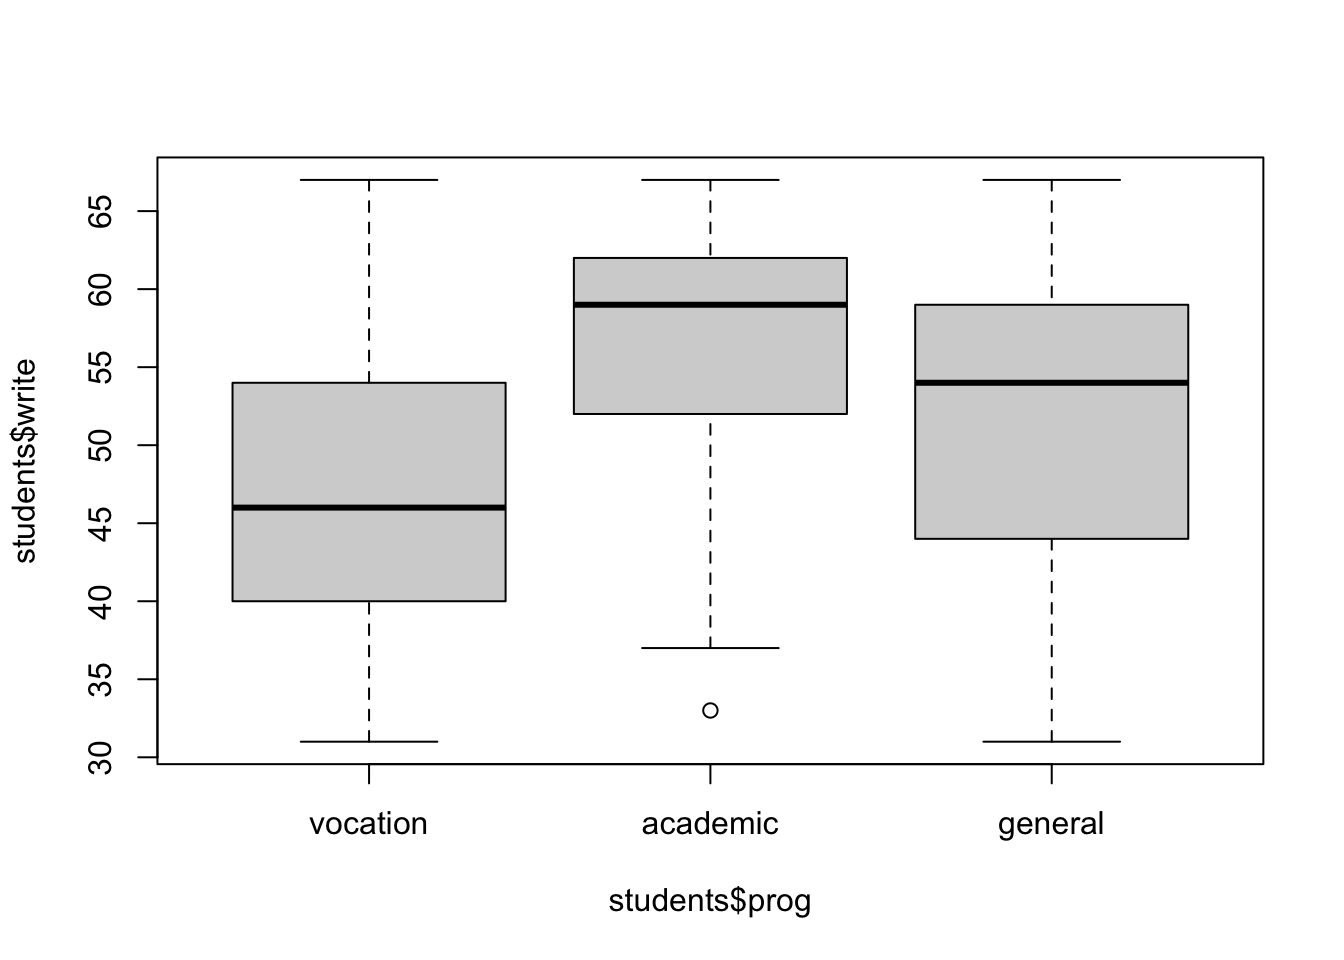
\includegraphics{smr_book_files/figure-latex/unnamed-chunk-163-1.pdf}

\begin{Shaded}
\begin{Highlighting}[]
\CommentTok{\# precise boundaries (numbers) are found with the \textasciigrave{}quantile()\textasciigrave{} function}
\FunctionTok{with}\NormalTok{(students, \{}
  \FunctionTok{quantile}\NormalTok{(write[prog }\SpecialCharTok{==} \StringTok{"vocation"}\NormalTok{], }\AttributeTok{prob =} \FunctionTok{seq}\NormalTok{(}\DecValTok{0}\NormalTok{, }\DecValTok{1}\NormalTok{, }\AttributeTok{by =}\NormalTok{ .}\DecValTok{25}\NormalTok{))}
\NormalTok{\})}
\end{Highlighting}
\end{Shaded}

\begin{verbatim}
##    0%   25%   50%   75%  100% 
## 31.00 40.25 46.00 53.50 67.00
\end{verbatim}

\begin{Shaded}
\begin{Highlighting}[]
\CommentTok{\# boxplot in ggplot}
\FunctionTok{library}\NormalTok{(ggplot2)}
\NormalTok{students }\SpecialCharTok{\%\textgreater{}\%}
  \FunctionTok{ggplot}\NormalTok{(}\FunctionTok{aes}\NormalTok{(prog, write)) }\SpecialCharTok{+}
  \FunctionTok{geom\_boxplot}\NormalTok{()}
\end{Highlighting}
\end{Shaded}

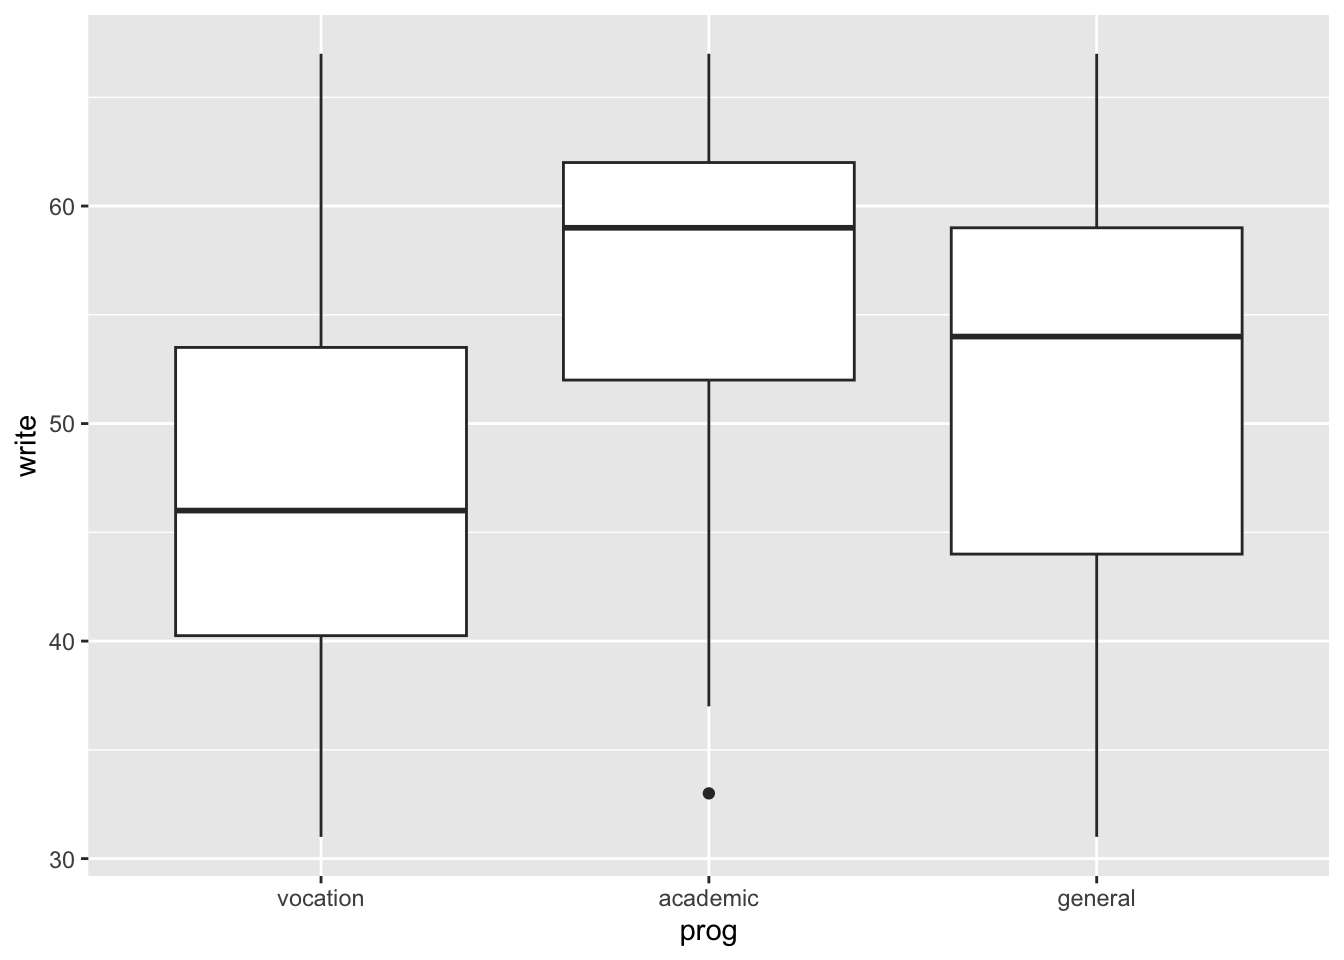
\includegraphics{smr_book_files/figure-latex/unnamed-chunk-165-1.pdf}

\begin{Shaded}
\begin{Highlighting}[]
\CommentTok{\# geom\_violin() \# try also the "violin plot"}
\end{Highlighting}
\end{Shaded}

We can also put all subjects together, but we need to
switch to long format with \texttt{gather} (or \texttt{reshape2::melt}).

\begin{Shaded}
\begin{Highlighting}[]
\CommentTok{\# view of the grades distribution depending}
\CommentTok{\# on subject and program}
\NormalTok{students }\SpecialCharTok{\%\textgreater{}\%}
  \FunctionTok{gather}\NormalTok{(}\AttributeTok{key =} \StringTok{"subject"}\NormalTok{, }\AttributeTok{value =} \StringTok{"grade"}\NormalTok{, write, science, math, read) }\SpecialCharTok{\%\textgreater{}\%}
  \FunctionTok{ggplot}\NormalTok{() }\SpecialCharTok{+}
  \FunctionTok{geom\_boxplot}\NormalTok{(}\FunctionTok{aes}\NormalTok{(prog, grade, }\AttributeTok{fill =}\NormalTok{ subject))}
\end{Highlighting}
\end{Shaded}

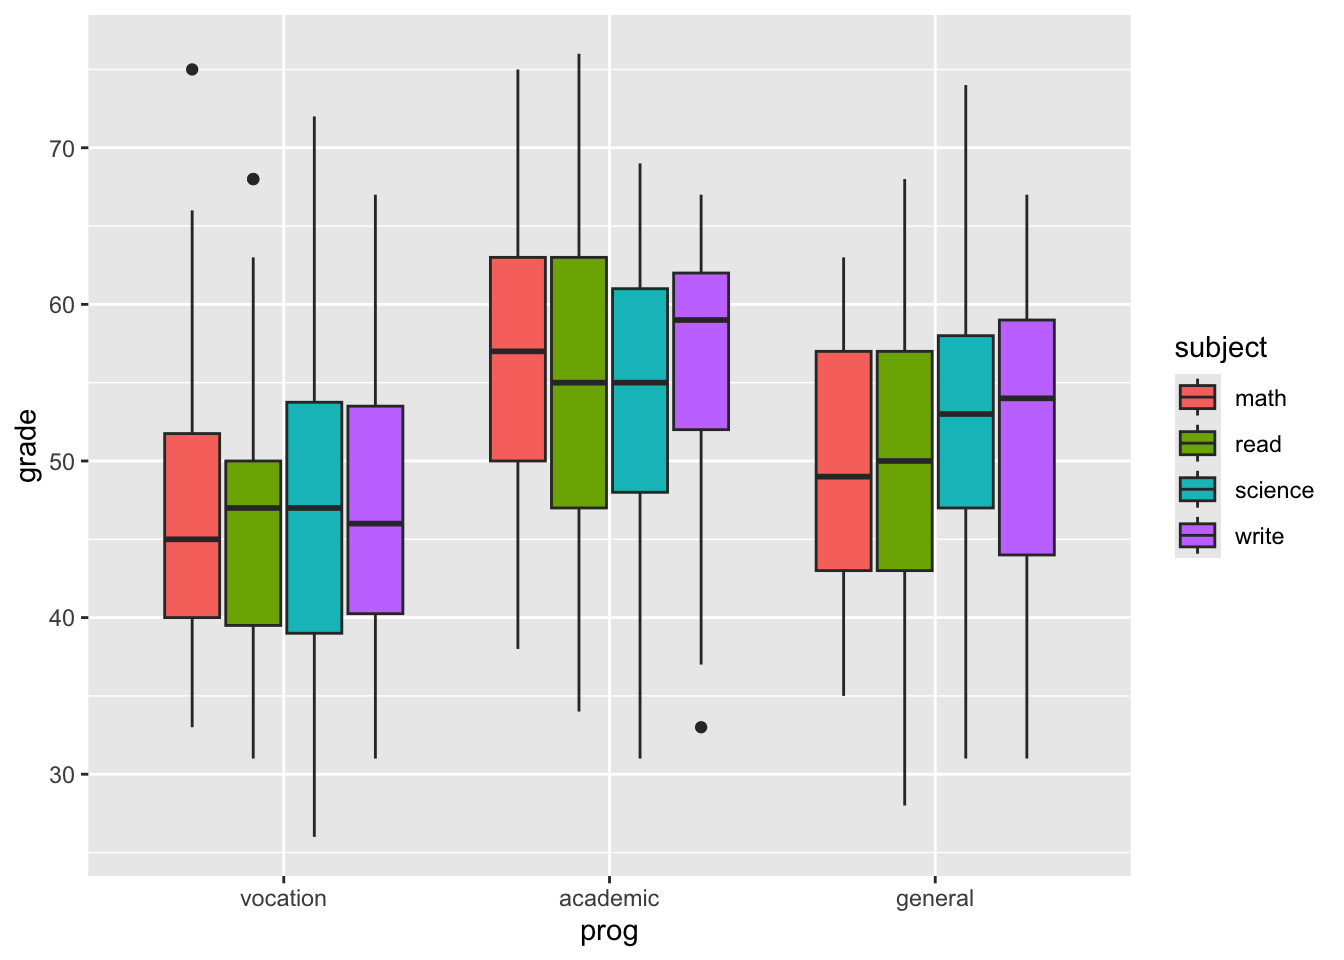
\includegraphics{smr_book_files/figure-latex/unnamed-chunk-166-1.pdf}

\begin{Shaded}
\begin{Highlighting}[]
\CommentTok{\# or in different plots with}
\CommentTok{\#    ...}
\CommentTok{\#    geom\_boxplot(aes(prog, grade)) +}
\CommentTok{\#    facet\_wrap(\textasciitilde{} subject) \# instead of}
\end{Highlighting}
\end{Shaded}

\section{Test}\label{test}

We can further analyse the dataset attributes with some tests and
traditional linear regression fit.

\begin{Shaded}
\begin{Highlighting}[]
\FunctionTok{with}\NormalTok{(students }\SpecialCharTok{\%\textgreater{}\%} \FunctionTok{filter}\NormalTok{(prog }\SpecialCharTok{!=} \StringTok{"vocation"}\NormalTok{), \{}
\NormalTok{  tt\_wp }\OtherTok{\textless{}{-}} \FunctionTok{t.test}\NormalTok{(write[prog }\SpecialCharTok{==} \StringTok{"general"}\NormalTok{], }\CommentTok{\# are the two prog distributed the same way?}
\NormalTok{    write[prog }\SpecialCharTok{==} \StringTok{"academic"}\NormalTok{],}
    \AttributeTok{var.equal =} \ConstantTok{TRUE}
\NormalTok{  )}
\NormalTok{  lm\_wp }\OtherTok{\textless{}{-}} \FunctionTok{summary}\NormalTok{(}\FunctionTok{lm}\NormalTok{(write }\SpecialCharTok{\textasciitilde{}}\NormalTok{ prog)) }\CommentTok{\# lm with qualitative predictor}
\NormalTok{  anova\_wp }\OtherTok{\textless{}{-}} \FunctionTok{summary}\NormalTok{(}\FunctionTok{aov}\NormalTok{(write }\SpecialCharTok{\textasciitilde{}}\NormalTok{ prog)) }\CommentTok{\# anova}
  \FunctionTok{list}\NormalTok{(tt\_wp, lm\_wp, anova\_wp)}
\NormalTok{\})}
\end{Highlighting}
\end{Shaded}

\begin{verbatim}
## [[1]]
## 
##  Two Sample t-test
## 
## data:  write[prog == "general"] and write[prog == "academic"]
## t = -3.289, df = 148, p-value = 0.001256
## alternative hypothesis: true difference in means is not equal to 0
## 95 percent confidence interval:
##  -7.882132 -1.965487
## sample estimates:
## mean of x mean of y 
##  51.33333  56.25714 
## 
## 
## [[2]]
## 
## Call:
## lm(formula = write ~ prog)
## 
## Residuals:
##     Min      1Q  Median      3Q     Max 
## -23.257  -4.257   2.705   5.743  15.667 
## 
## Coefficients:
##             Estimate Std. Error t value Pr(>|t|)    
## (Intercept)   56.257      0.820  68.610  < 2e-16 ***
## proggeneral   -4.924      1.497  -3.289  0.00126 ** 
## ---
## Signif. codes:  0 '***' 0.001 '**' 0.01 '*' 0.05 '.' 0.1 ' ' 1
## 
## Residual standard error: 8.402 on 148 degrees of freedom
## Multiple R-squared:  0.06811,    Adjusted R-squared:  0.06182 
## F-statistic: 10.82 on 1 and 148 DF,  p-value: 0.001256
## 
## 
## [[3]]
##              Df Sum Sq Mean Sq F value  Pr(>F)   
## prog          1    764   763.7   10.82 0.00126 **
## Residuals   148  10448    70.6                   
## ---
## Signif. codes:  0 '***' 0.001 '**' 0.01 '*' 0.05 '.' 0.1 ' ' 1
\end{verbatim}

Notice how the T-test t-value is equal to the linear model coefficient estimate t-value.
They are computed the same way.

\section{Generalized Linear Model}\label{generalized-linear-model}

The \(X\)s have to be independent, thus we check the correlation plots.

\begin{Shaded}
\begin{Highlighting}[]
\FunctionTok{library}\NormalTok{(GGally)}
\NormalTok{students }\SpecialCharTok{\%\textgreater{}\%}
\NormalTok{  dplyr}\SpecialCharTok{::}\FunctionTok{select}\NormalTok{(math, science, write, read) }\SpecialCharTok{\%\textgreater{}\%}
  \FunctionTok{ggpairs}\NormalTok{(}\AttributeTok{progress =} \ConstantTok{FALSE}\NormalTok{)}
\end{Highlighting}
\end{Shaded}

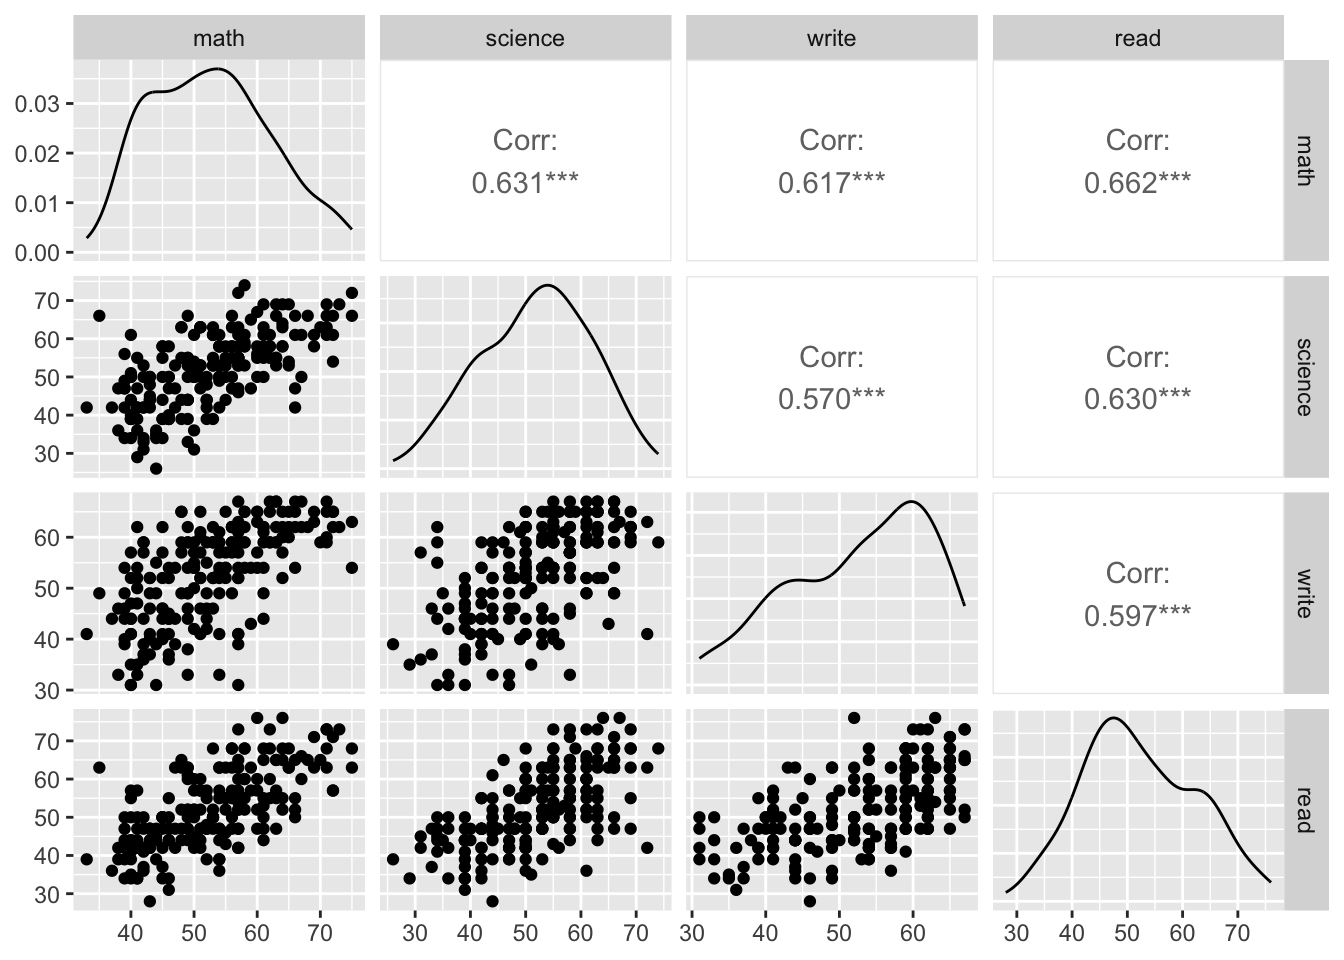
\includegraphics{smr_book_files/figure-latex/unnamed-chunk-168-1.pdf}

In order to be able to use the Binomial generalized linear model
and set the program as response variable, we have to make a new
dataset in which we define a binary class instead of a three levels
factor. Here we arbitrarily choose to create a variable which is
1 for \texttt{vocation} and 0 for \texttt{general}.

\begin{Shaded}
\begin{Highlighting}[]
\CommentTok{\# create a new dataframe}
\NormalTok{students\_vg }\OtherTok{\textless{}{-}}\NormalTok{ students }\SpecialCharTok{\%\textgreater{}\%}
  \FunctionTok{filter}\NormalTok{(prog }\SpecialCharTok{!=} \StringTok{"academic"}\NormalTok{) }\SpecialCharTok{\%\textgreater{}\%} \CommentTok{\# make distinction vocation{-}general only}
  \FunctionTok{mutate}\NormalTok{(}\AttributeTok{vocation =} \FunctionTok{ifelse}\NormalTok{(prog }\SpecialCharTok{==} \StringTok{"vocation"}\NormalTok{, }\DecValTok{1}\NormalTok{, }\DecValTok{0}\NormalTok{)) }\CommentTok{\# transform class to binary}

\NormalTok{voc\_glm }\OtherTok{\textless{}{-}} \FunctionTok{glm}\NormalTok{(vocation }\SpecialCharTok{\textasciitilde{}}\NormalTok{ ses }\SpecialCharTok{+}\NormalTok{ schtyp }\SpecialCharTok{+}\NormalTok{ read }\SpecialCharTok{+}\NormalTok{ write }\SpecialCharTok{+}\NormalTok{ math, }\CommentTok{\# choose some predictors}
  \AttributeTok{data =}\NormalTok{ students\_vg, }\AttributeTok{family =} \StringTok{"binomial"}
\NormalTok{) }\CommentTok{\# fit glm with binomial link}
\end{Highlighting}
\end{Shaded}

\begin{Shaded}
\begin{Highlighting}[]
\CommentTok{\# new pipe operator (base R 4.2 or later) allows to send}
\CommentTok{\# pipe results to any function parameter (not just the first one)}
\CommentTok{\# and it\textquotesingle{}s compatible with lm/glm calls (no need to create new datasets)}
\NormalTok{voc\_glm }\OtherTok{\textless{}{-}}\NormalTok{ students }\SpecialCharTok{|\textgreater{}}
  \FunctionTok{filter}\NormalTok{(prog }\SpecialCharTok{!=} \StringTok{"academic"}\NormalTok{) }\SpecialCharTok{|\textgreater{}}
  \FunctionTok{mutate}\NormalTok{(}\AttributeTok{vocation =} \FunctionTok{ifelse}\NormalTok{(prog }\SpecialCharTok{==} \StringTok{"vocation"}\NormalTok{, }\DecValTok{1}\NormalTok{, }\DecValTok{0}\NormalTok{)) }\SpecialCharTok{|\textgreater{}}
  \FunctionTok{glm}\NormalTok{(vocation }\SpecialCharTok{\textasciitilde{}}\NormalTok{ ses }\SpecialCharTok{+}\NormalTok{ schtyp }\SpecialCharTok{+}\NormalTok{ read }\SpecialCharTok{+}\NormalTok{ write }\SpecialCharTok{+}\NormalTok{ math,}
    \AttributeTok{data =}\NormalTok{ \_, }\AttributeTok{family =} \StringTok{"binomial"}
\NormalTok{  )}
\CommentTok{\# \textasciigrave{}\_\textasciigrave{} is placeholder for the piped dataframe}
\end{Highlighting}
\end{Shaded}

\begin{Shaded}
\begin{Highlighting}[]
\FunctionTok{summary}\NormalTok{(voc\_glm)}
\end{Highlighting}
\end{Shaded}

\begin{verbatim}
## 
## Call:
## glm(formula = vocation ~ ses + schtyp + read + write + math, 
##     family = "binomial", data = students_vg)
## 
## Coefficients:
##               Estimate Std. Error z value Pr(>|z|)  
## (Intercept)    3.78961    1.62184   2.337   0.0195 *
## sesmiddle      1.04148    0.53206   1.957   0.0503 .
## seshigh        0.42122    0.68145   0.618   0.5365  
## schtypprivate -1.06617    0.87344  -1.221   0.2222  
## read          -0.02558    0.02940  -0.870   0.3843  
## write         -0.02011    0.02836  -0.709   0.4782  
## math          -0.04175    0.03438  -1.214   0.2246  
## ---
## Signif. codes:  0 '***' 0.001 '**' 0.01 '*' 0.05 '.' 0.1 ' ' 1
## 
## (Dispersion parameter for binomial family taken to be 1)
## 
##     Null deviance: 131.43  on 94  degrees of freedom
## Residual deviance: 118.24  on 88  degrees of freedom
## AIC: 132.24
## 
## Number of Fisher Scoring iterations: 4
\end{verbatim}

In the summary output, few differences from the \texttt{lm} call
can be noticed:

\begin{itemize}
\tightlist
\item
  the p-value for each coefficient is determined through a z-test
  instead of an exact t-test;
\item
  R-squared cannot be computed (there are no residuals) and the
  \emph{deviance} is printed instead:

  \begin{itemize}
  \tightlist
  \item
    \texttt{Null\ deviance} represents the distance of the null model
    (which has only the intercept) from a ``perfect'' saturated model
  \item
    \texttt{Residual\ deviance} compares the fit with the saturated model (with number
    of parameters equal to the number of observations)
  \end{itemize}
\end{itemize}

We can do the same thing with the pair \texttt{academic/general}.

\begin{Shaded}
\begin{Highlighting}[]
\NormalTok{students\_ag }\OtherTok{\textless{}{-}}\NormalTok{ students }\SpecialCharTok{\%\textgreater{}\%}
  \FunctionTok{filter}\NormalTok{(prog }\SpecialCharTok{!=} \StringTok{"vocation"}\NormalTok{) }\SpecialCharTok{\%\textgreater{}\%}
  \FunctionTok{mutate}\NormalTok{(}\AttributeTok{academic =} \FunctionTok{ifelse}\NormalTok{(prog }\SpecialCharTok{==} \StringTok{"academic"}\NormalTok{, }\DecValTok{1}\NormalTok{, }\DecValTok{0}\NormalTok{))}

\NormalTok{academic\_glm }\OtherTok{\textless{}{-}} \FunctionTok{glm}\NormalTok{(academic }\SpecialCharTok{\textasciitilde{}}\NormalTok{ ses }\SpecialCharTok{+}\NormalTok{ schtyp }\SpecialCharTok{+}\NormalTok{ read }\SpecialCharTok{+}\NormalTok{ write }\SpecialCharTok{+}\NormalTok{ math, }\CommentTok{\# same predictors}
  \AttributeTok{data =}\NormalTok{ students\_ag, }\AttributeTok{family =} \StringTok{"binomial"}
\NormalTok{)}
\FunctionTok{summary}\NormalTok{(academic\_glm)}
\end{Highlighting}
\end{Shaded}

\begin{verbatim}
## 
## Call:
## glm(formula = academic ~ ses + schtyp + read + write + math, 
##     family = "binomial", data = students_ag)
## 
## Coefficients:
##               Estimate Std. Error z value Pr(>|z|)    
## (Intercept)   -5.07477    1.47499  -3.441 0.000581 ***
## sesmiddle      0.23316    0.47768   0.488 0.625471    
## seshigh        0.77579    0.54950   1.412 0.158004    
## schtypprivate  0.61998    0.53668   1.155 0.248007    
## read           0.02441    0.02793   0.874 0.382069    
## write          0.01130    0.02753   0.411 0.681416    
## math           0.06720    0.03164   2.124 0.033689 *  
## ---
## Signif. codes:  0 '***' 0.001 '**' 0.01 '*' 0.05 '.' 0.1 ' ' 1
## 
## (Dispersion parameter for binomial family taken to be 1)
## 
##     Null deviance: 183.26  on 149  degrees of freedom
## Residual deviance: 157.94  on 143  degrees of freedom
## AIC: 171.94
## 
## Number of Fisher Scoring iterations: 4
\end{verbatim}

Of course, we get different coefficient estimates with different models.
We can compare them:

\begin{Shaded}
\begin{Highlighting}[]
\FunctionTok{cbind}\NormalTok{(}
  \FunctionTok{summary}\NormalTok{(voc\_glm)}\SpecialCharTok{$}\NormalTok{coefficients[, }\FunctionTok{c}\NormalTok{(}\DecValTok{1}\NormalTok{, }\DecValTok{4}\NormalTok{)],}
  \FunctionTok{summary}\NormalTok{(academic\_glm)}\SpecialCharTok{$}\NormalTok{coefficients[, }\FunctionTok{c}\NormalTok{(}\DecValTok{1}\NormalTok{, }\DecValTok{4}\NormalTok{)]}
\NormalTok{)}
\end{Highlighting}
\end{Shaded}

\begin{verbatim}
##                  Estimate   Pr(>|z|)    Estimate     Pr(>|z|)
## (Intercept)    3.78961265 0.01945937 -5.07476526 0.0005805405
## sesmiddle      1.04148131 0.05029279  0.23316035 0.6254706198
## seshigh        0.42121982 0.53649208  0.77579361 0.1580040841
## schtypprivate -1.06616814 0.22221864  0.61997866 0.2480066053
## read          -0.02557603 0.38428691  0.02441089 0.3820686083
## write         -0.02011257 0.47821104  0.01130034 0.6814162867
## math          -0.04175324 0.22462769  0.06720110 0.0336894120
\end{verbatim}

Let's use \texttt{step} to chose the minimal set of useful predictors:
it analyzes AIC for each combination of predictors, by progressively
fitting a model with less and less predictors. The way it proceeds is the
following:

\begin{enumerate}
\def\labelenumi{\arabic{enumi}.}
\tightlist
\item
  fit the complete model,
\item
  for each of the predictors, fit another model with all but that predictor,
\item
  compare the AIC of all these models (\texttt{\textless{}none\textgreater{}} is the complete) and keep the
  one with the highest AIC;
\item
  repeat until the best model is found (i.e.~\texttt{\textless{}none\textgreater{}} has highest AIC
  score)
\end{enumerate}

Notice how this procedure can lead to sub-optimal models, since it doesn't try
all possible predictors combinations, but rather finds a greedy solution to this
search.

\begin{Shaded}
\begin{Highlighting}[]
\NormalTok{?step}
\end{Highlighting}
\end{Shaded}

\begin{Shaded}
\begin{Highlighting}[]
\NormalTok{step\_voc }\OtherTok{\textless{}{-}} \FunctionTok{step}\NormalTok{(voc\_glm)}
\end{Highlighting}
\end{Shaded}

\begin{verbatim}
## Start:  AIC=132.24
## vocation ~ ses + schtyp + read + write + math
## 
##          Df Deviance    AIC
## - write   1   118.74 130.74
## - read    1   119.00 131.00
## - math    1   119.75 131.75
## - schtyp  1   119.90 131.90
## <none>        118.24 132.24
## - ses     2   122.42 132.42
## 
## Step:  AIC=130.74
## vocation ~ ses + schtyp + read + math
## 
##          Df Deviance    AIC
## - read    1   120.25 130.25
## - schtyp  1   120.64 130.64
## <none>        118.74 130.74
## - math    1   121.07 131.07
## - ses     2   123.60 131.60
## 
## Step:  AIC=130.25
## vocation ~ ses + schtyp + math
## 
##          Df Deviance    AIC
## - schtyp  1   122.23 130.23
## <none>        120.25 130.25
## - ses     2   124.51 130.51
## - math    1   125.30 133.30
## 
## Step:  AIC=130.23
## vocation ~ ses + math
## 
##        Df Deviance    AIC
## <none>      122.23 130.23
## - ses   2   126.33 130.33
## - math  1   128.48 134.48
\end{verbatim}

\begin{Shaded}
\begin{Highlighting}[]
\FunctionTok{summary}\NormalTok{(step\_voc)}
\end{Highlighting}
\end{Shaded}

\begin{verbatim}
## 
## Call:
## glm(formula = vocation ~ ses + math, family = "binomial", data = students_vg)
## 
## Coefficients:
##             Estimate Std. Error z value Pr(>|z|)  
## (Intercept)  2.97676    1.41738   2.100   0.0357 *
## sesmiddle    0.97663    0.50784   1.923   0.0545 .
## seshigh      0.34949    0.66611   0.525   0.5998  
## math        -0.07160    0.03016  -2.374   0.0176 *
## ---
## Signif. codes:  0 '***' 0.001 '**' 0.01 '*' 0.05 '.' 0.1 ' ' 1
## 
## (Dispersion parameter for binomial family taken to be 1)
## 
##     Null deviance: 131.43  on 94  degrees of freedom
## Residual deviance: 122.23  on 91  degrees of freedom
## AIC: 130.23
## 
## Number of Fisher Scoring iterations: 4
\end{verbatim}

\begin{Shaded}
\begin{Highlighting}[]
\CommentTok{\# run this and check the results}
\NormalTok{step\_academic }\OtherTok{\textless{}{-}} \FunctionTok{step}\NormalTok{(academic\_glm)}
\FunctionTok{summary}\NormalTok{(step\_academic)}
\end{Highlighting}
\end{Shaded}

\subsection{Predictions}\label{predictions}

Working with generalized linear models, we can choose whether to get the
logit estimate

\[
g(\mu) = \eta = X \hat\beta
\]

or the response probabilities, which is simply the inverse of the logit.

\begin{Shaded}
\begin{Highlighting}[]
\FunctionTok{head}\NormalTok{(voc\_glm}\SpecialCharTok{$}\NormalTok{fitted.values)}
\end{Highlighting}
\end{Shaded}

\begin{verbatim}
##         1         2         3         4         5         6 
## 0.5902369 0.8363280 0.6098686 0.6217618 0.7541615 0.7456350
\end{verbatim}

\begin{Shaded}
\begin{Highlighting}[]
\FunctionTok{head}\NormalTok{(}\FunctionTok{predict}\NormalTok{(voc\_glm, }\AttributeTok{newdata =}\NormalTok{ students, }\AttributeTok{type =} \StringTok{"response"}\NormalTok{)) }\CommentTok{\# probs}
\end{Highlighting}
\end{Shaded}

\begin{verbatim}
##         1         2         3         4         5         6 
## 0.5902369 0.8363280 0.2435802 0.4866921 0.4969118 0.4606502
\end{verbatim}

\begin{Shaded}
\begin{Highlighting}[]
\FunctionTok{head}\NormalTok{(}\FunctionTok{predict}\NormalTok{(voc\_glm, }\AttributeTok{newdata =}\NormalTok{ students)) }\CommentTok{\# logit}
\end{Highlighting}
\end{Shaded}

\begin{verbatim}
##           1           2           3           4           5           6 
##  0.36494483  1.63115634 -1.13315009 -0.05324419 -0.01235304 -0.15772532
\end{verbatim}

\begin{quote}
Exercise: compute the inverse of the logit (manually) and verify that
it equals the response found with \texttt{predict} (solution is in the Rmarkdown
file).
\end{quote}

The reason why we fitted two complementary models, is that we can combine
the results to obtain predictions for both three programs together.

The logits are so defined for the two models:
\[
X_{vg}\beta_{vg} = \log\left(\frac{\pi_{v}}{\pi_g}\right)\,,\\
X_{ag}\beta_{ag} = \log\left(\frac{\pi_{a}}{\pi_g}\right)\,,
\]

and knowing that \(\pi_v + \pi_g + \pi_a = 1\)
we have

\[
\pi_g = \left(\frac{\pi_v}{\pi_g} + \frac{\pi_a}{\pi_g} + 1\right)^{-1}\,.
\]

With some manipulation, replacing this result in the
logits above, we can show that, for each class \(v, g, a\):

\[
\pi_v = \frac{e^{X_{vg}\beta_{vg}}}{1 + e^{X_{vg}\beta_{vg}} + e^{X_{ag}\beta_{ag}}}\,.
\]

This formula is also called \emph{softmax}, which converts numbers to probabilities (instead
of just taking the max index, ``hard''-max) and makes it possible to generalize
from logistic regression to multiple category regression, sometimes
called, indeed, \emph{softmax regression}.

Let's do this in R

\begin{Shaded}
\begin{Highlighting}[]
\NormalTok{exp\_voc }\OtherTok{\textless{}{-}} \FunctionTok{exp}\NormalTok{(}\FunctionTok{predict}\NormalTok{(voc\_glm, }\AttributeTok{type =} \StringTok{"link"}\NormalTok{, }\AttributeTok{newdata =}\NormalTok{ students))}
\NormalTok{exp\_academic }\OtherTok{\textless{}{-}} \FunctionTok{exp}\NormalTok{(}\FunctionTok{predict}\NormalTok{(academic\_glm, }\AttributeTok{type =} \StringTok{"link"}\NormalTok{, }\AttributeTok{newdata =}\NormalTok{ students))}
\end{Highlighting}
\end{Shaded}

\begin{Shaded}
\begin{Highlighting}[]
\NormalTok{norm\_const }\OtherTok{\textless{}{-}} \DecValTok{1} \SpecialCharTok{+}\NormalTok{ exp\_voc }\SpecialCharTok{+}\NormalTok{ exp\_academic}
\NormalTok{pred }\OtherTok{\textless{}{-}} \FunctionTok{tibble}\NormalTok{(}
  \AttributeTok{pred\_gen =} \DecValTok{1}\NormalTok{, }\AttributeTok{pred\_voc =}\NormalTok{ exp\_voc,}
  \AttributeTok{pred\_acad =}\NormalTok{ exp\_academic}
\NormalTok{) }\SpecialCharTok{/}\NormalTok{ norm\_const}
\FunctionTok{head}\NormalTok{(pred)}
\end{Highlighting}
\end{Shaded}

\begin{verbatim}
##    pred_gen  pred_voc  pred_acad
## 1 0.3588022 0.5168311 0.12436676
## 2 0.1560455 0.7973583 0.04659614
## 3 0.3510001 0.1130281 0.53597187
## 4 0.4074066 0.3862819 0.20631153
## 5 0.3930219 0.3881968 0.21878130
## 6 0.3932633 0.3358800 0.27085675
\end{verbatim}

Predictions must sum to 1 (they're normalized).

\begin{Shaded}
\begin{Highlighting}[]
\FunctionTok{rowSums}\NormalTok{(pred)}
\end{Highlighting}
\end{Shaded}

\begin{verbatim}
##   [1] 1 1 1 1 1 1 1 1 1 1 1 1 1 1 1 1 1 1 1 1 1 1 1 1 1 1 1 1 1 1 1 1 1 1 1 1 1
##  [38] 1 1 1 1 1 1 1 1 1 1 1 1 1 1 1 1 1 1 1 1 1 1 1 1 1 1 1 1 1 1 1 1 1 1 1 1 1
##  [75] 1 1 1 1 1 1 1 1 1 1 1 1 1 1 1 1 1 1 1 1 1 1 1 1 1 1 1 1 1 1 1 1 1 1 1 1 1
## [112] 1 1 1 1 1 1 1 1 1 1 1 1 1 1 1 1 1 1 1 1 1 1 1 1 1 1 1 1 1 1 1 1 1 1 1 1 1
## [149] 1 1 1 1 1 1 1 1 1 1 1 1 1 1 1 1 1 1 1 1 1 1 1 1 1 1 1 1 1 1 1 1 1 1 1 1 1
## [186] 1 1 1 1 1 1 1 1 1 1 1 1 1 1 1
\end{verbatim}

\section{Graphic interpretation}\label{graphic-interpretation}

These are some of the ways we can visualize the results.
The plots interpretation is left as exercise.

\begin{Shaded}
\begin{Highlighting}[]
\NormalTok{pred\_stud\_long }\OtherTok{\textless{}{-}} \FunctionTok{bind\_cols}\NormalTok{(pred, students) }\SpecialCharTok{\%\textgreater{}\%}
  \FunctionTok{gather}\NormalTok{(}\AttributeTok{key =} \StringTok{"predProg"}\NormalTok{, }\AttributeTok{value =} \StringTok{"prediction"}\NormalTok{, pred\_gen}\SpecialCharTok{:}\NormalTok{pred\_acad)}

\NormalTok{pred\_stud\_long }\SpecialCharTok{\%\textgreater{}\%}
  \FunctionTok{ggplot}\NormalTok{() }\SpecialCharTok{+}
  \FunctionTok{geom\_point}\NormalTok{(}\FunctionTok{aes}\NormalTok{(write, prediction, }\AttributeTok{color =}\NormalTok{ predProg))}
\end{Highlighting}
\end{Shaded}

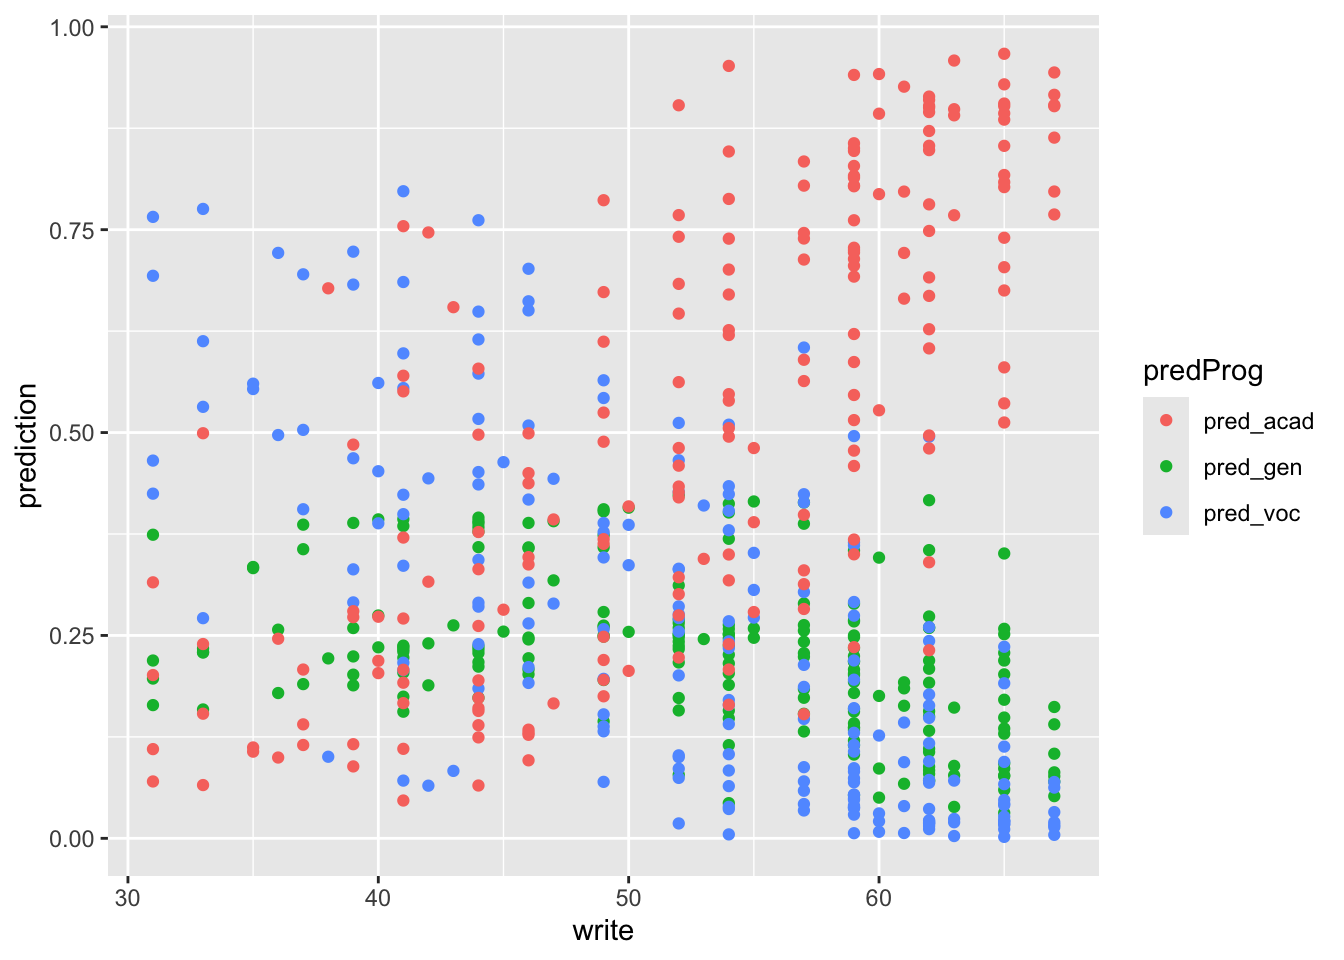
\includegraphics{smr_book_files/figure-latex/unnamed-chunk-183-1.pdf}

\begin{Shaded}
\begin{Highlighting}[]
\NormalTok{pred\_stud\_long }\SpecialCharTok{\%\textgreater{}\%}
  \FunctionTok{ggplot}\NormalTok{() }\SpecialCharTok{+}
  \FunctionTok{geom\_point}\NormalTok{(}\FunctionTok{aes}\NormalTok{(math, prediction, }\AttributeTok{color =}\NormalTok{ predProg))}
\end{Highlighting}
\end{Shaded}

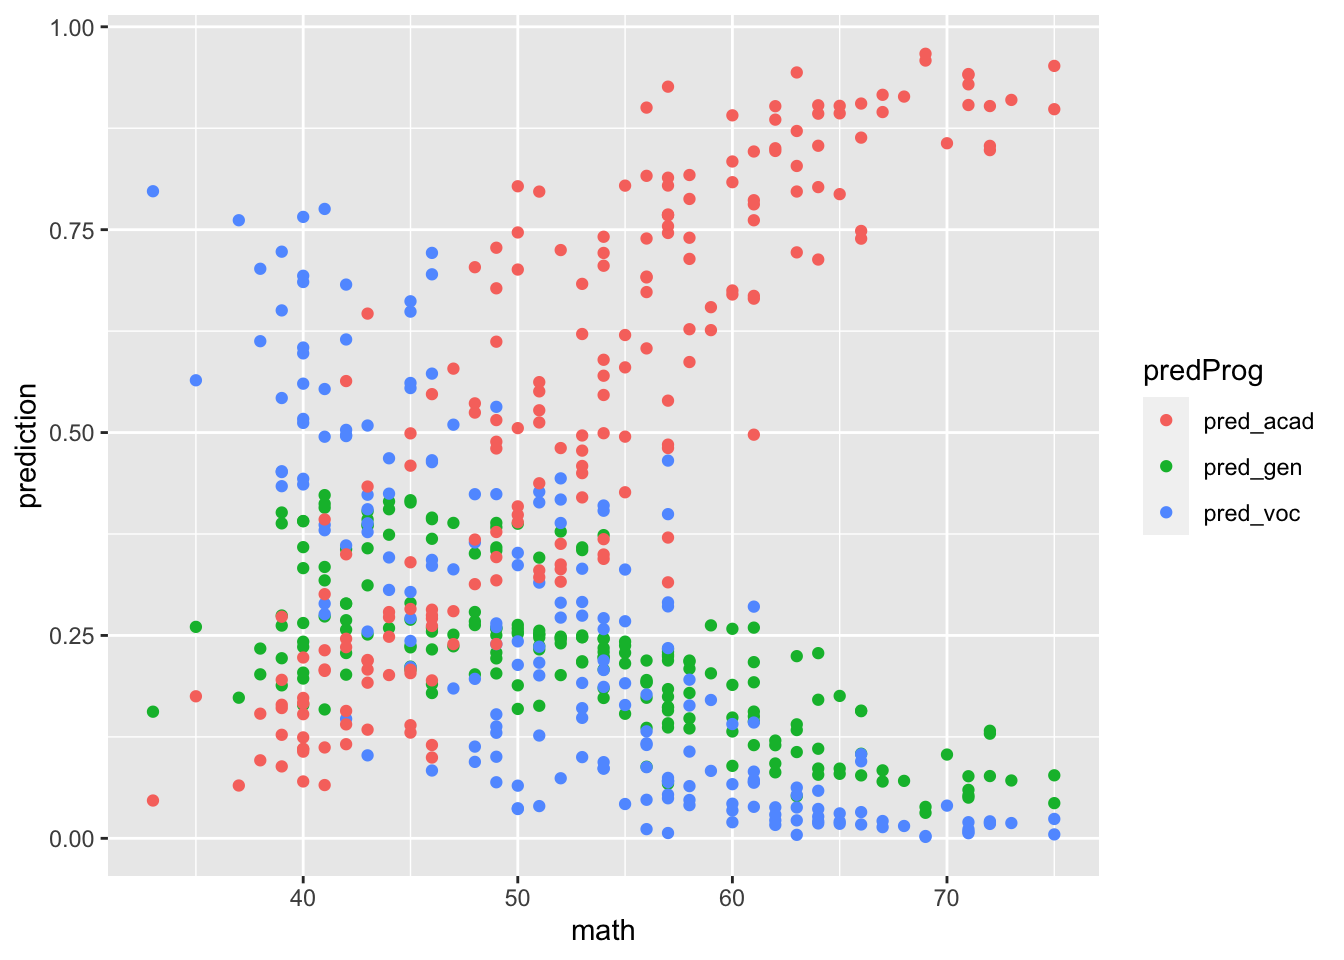
\includegraphics{smr_book_files/figure-latex/unnamed-chunk-184-1.pdf}

\begin{Shaded}
\begin{Highlighting}[]
\NormalTok{pred\_stud\_long }\SpecialCharTok{\%\textgreater{}\%}
  \FunctionTok{ggplot}\NormalTok{() }\SpecialCharTok{+}
  \FunctionTok{geom\_boxplot}\NormalTok{(}\FunctionTok{aes}\NormalTok{(ses, prediction, }\AttributeTok{color =}\NormalTok{ ses)) }\SpecialCharTok{+}
  \FunctionTok{facet\_wrap}\NormalTok{(}\SpecialCharTok{\textasciitilde{}}\NormalTok{predProg)}
\end{Highlighting}
\end{Shaded}

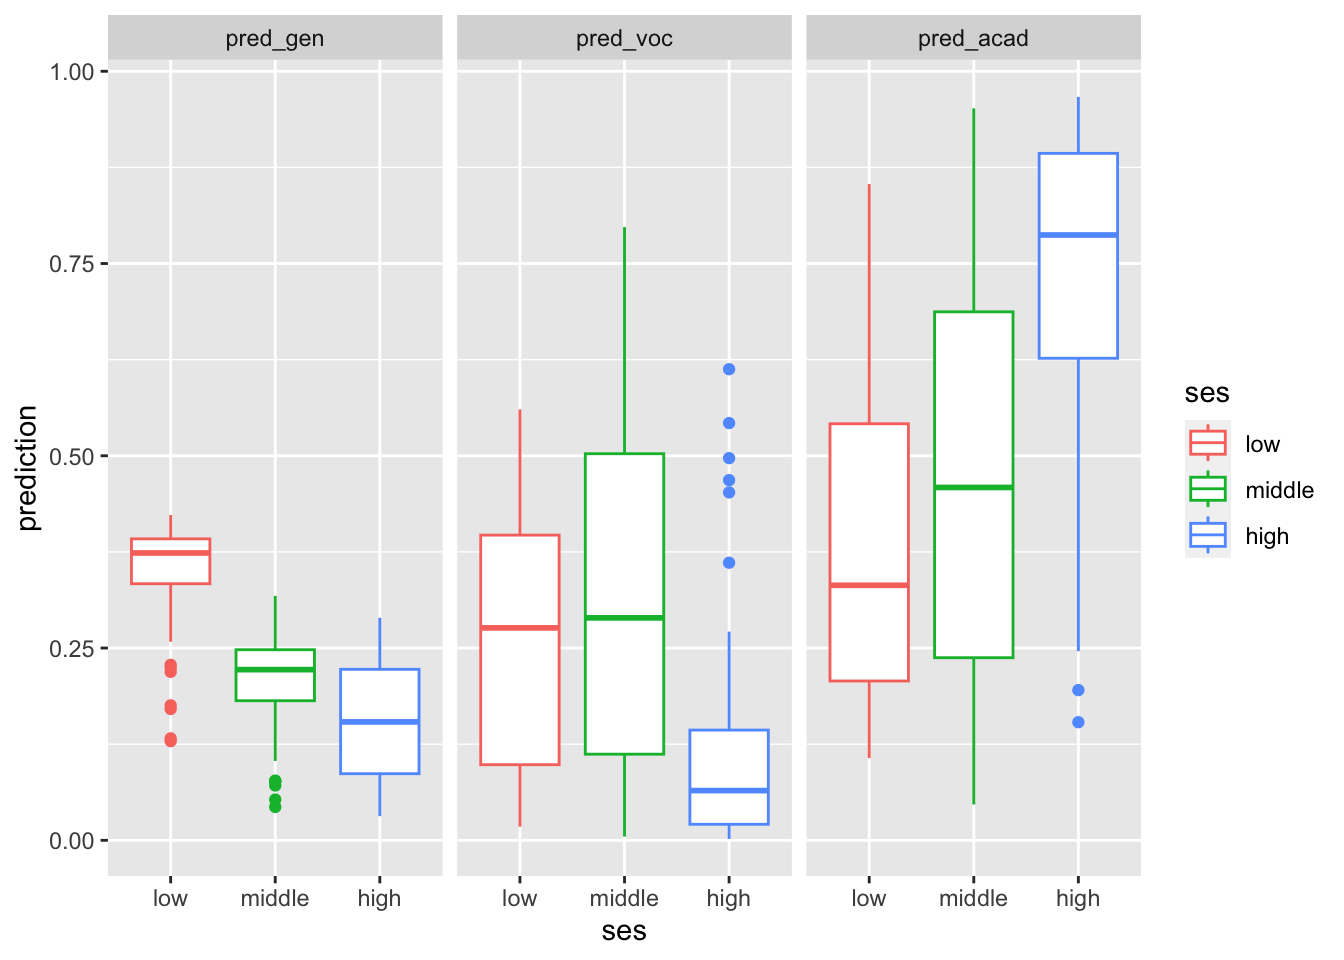
\includegraphics{smr_book_files/figure-latex/unnamed-chunk-185-1.pdf}

\section{Other tests}\label{other-tests}

The models fitted so fare are not the only one that can give
insights on the data. Here's some other models and tests made with
arbitrary data.
Feel free to further experiment the dataset.

\begin{Shaded}
\begin{Highlighting}[]
\CommentTok{\# to run this, make sure you have R 4.2 installed.}
\CommentTok{\# otherwise use the alternative way shown in the section above}
\NormalTok{general\_glm }\OtherTok{\textless{}{-}}\NormalTok{ students }\SpecialCharTok{|\textgreater{}}
  \FunctionTok{mutate}\NormalTok{(}\AttributeTok{general =} \FunctionTok{ifelse}\NormalTok{(prog }\SpecialCharTok{==} \StringTok{"general"}\NormalTok{, }\DecValTok{1}\NormalTok{, }\DecValTok{0}\NormalTok{)) }\SpecialCharTok{|\textgreater{}}
  \FunctionTok{glm}\NormalTok{(general }\SpecialCharTok{\textasciitilde{}}\NormalTok{ ses }\SpecialCharTok{+}\NormalTok{ schtyp }\SpecialCharTok{+}\NormalTok{ read }\SpecialCharTok{+}\NormalTok{ write }\SpecialCharTok{+}\NormalTok{ math,}
    \AttributeTok{data =}\NormalTok{ \_, }\AttributeTok{family =} \StringTok{"binomial"}
\NormalTok{  )}
\FunctionTok{summary}\NormalTok{(general\_glm)}
\end{Highlighting}
\end{Shaded}

\begin{verbatim}
## 
## Call:
## glm(formula = general ~ ses + schtyp + read + write + math, family = "binomial", 
##     data = mutate(students, general = ifelse(prog == "general", 
##         1, 0)))
## 
## Coefficients:
##                Estimate Std. Error z value Pr(>|z|)
## (Intercept)    0.888726   1.139382   0.780    0.435
## sesmiddle     -0.548233   0.411069  -1.334    0.182
## seshigh       -0.787325   0.503662  -1.563    0.118
## schtypprivate -0.050761   0.507839  -0.100    0.920
## read          -0.011416   0.024227  -0.471    0.637
## write          0.009743   0.024416   0.399    0.690
## math          -0.030597   0.027101  -1.129    0.259
## 
## (Dispersion parameter for binomial family taken to be 1)
## 
##     Null deviance: 213.27  on 199  degrees of freedom
## Residual deviance: 205.11  on 193  degrees of freedom
## AIC: 219.11
## 
## Number of Fisher Scoring iterations: 4
\end{verbatim}

\begin{Shaded}
\begin{Highlighting}[]
\NormalTok{general\_alt\_glm }\OtherTok{\textless{}{-}}\NormalTok{ students }\SpecialCharTok{|\textgreater{}} \CommentTok{\# notice no filter on prog != "academic"}
  \FunctionTok{mutate}\NormalTok{(}\AttributeTok{general =} \FunctionTok{ifelse}\NormalTok{(prog }\SpecialCharTok{==} \StringTok{"vocation"}\NormalTok{, }\DecValTok{1}\NormalTok{, }\DecValTok{0}\NormalTok{)) }\SpecialCharTok{|\textgreater{}}
  \FunctionTok{glm}\NormalTok{(general }\SpecialCharTok{\textasciitilde{}}\NormalTok{ ses }\SpecialCharTok{+}\NormalTok{ read }\SpecialCharTok{+}\NormalTok{ write }\SpecialCharTok{+}\NormalTok{ math,}
    \AttributeTok{data =}\NormalTok{ \_, }\AttributeTok{family =} \StringTok{"binomial"}
\NormalTok{  )}
\FunctionTok{summary}\NormalTok{(general\_alt\_glm)}
\end{Highlighting}
\end{Shaded}

\begin{verbatim}
## 
## Call:
## glm(formula = general ~ ses + read + write + math, family = "binomial", 
##     data = mutate(students, general = ifelse(prog == "vocation", 
##         1, 0)))
## 
## Coefficients:
##             Estimate Std. Error z value Pr(>|z|)    
## (Intercept)  6.11922    1.38391   4.422 9.79e-06 ***
## sesmiddle    0.83768    0.45392   1.845   0.0650 .  
## seshigh     -0.12410    0.58500  -0.212   0.8320    
## read        -0.03261    0.02672  -1.220   0.2223    
## write       -0.04151    0.02452  -1.693   0.0904 .  
## math        -0.07799    0.03054  -2.554   0.0107 *  
## ---
## Signif. codes:  0 '***' 0.001 '**' 0.01 '*' 0.05 '.' 0.1 ' ' 1
## 
## (Dispersion parameter for binomial family taken to be 1)
## 
##     Null deviance: 224.93  on 199  degrees of freedom
## Residual deviance: 179.08  on 194  degrees of freedom
## AIC: 191.08
## 
## Number of Fisher Scoring iterations: 5
\end{verbatim}

\begin{Shaded}
\begin{Highlighting}[]
\NormalTok{testdata }\OtherTok{\textless{}{-}} \FunctionTok{tibble}\NormalTok{(}
  \AttributeTok{ses =} \FunctionTok{c}\NormalTok{(}\StringTok{"low"}\NormalTok{, }\StringTok{"middle"}\NormalTok{, }\StringTok{"high"}\NormalTok{),}
  \AttributeTok{write =} \FunctionTok{mean}\NormalTok{(students}\SpecialCharTok{$}\NormalTok{write),}
  \AttributeTok{math =} \FunctionTok{mean}\NormalTok{(students}\SpecialCharTok{$}\NormalTok{math),}
  \AttributeTok{read =} \FunctionTok{mean}\NormalTok{(students}\SpecialCharTok{$}\NormalTok{read)}
\NormalTok{)}
\NormalTok{testdata }\SpecialCharTok{\%\textgreater{}\%}
  \FunctionTok{mutate}\NormalTok{(}\AttributeTok{prob =} \FunctionTok{predict}\NormalTok{(general\_alt\_glm, }\AttributeTok{newdata =}\NormalTok{ testdata, }\AttributeTok{type =} \StringTok{"response"}\NormalTok{))}
\end{Highlighting}
\end{Shaded}

\begin{verbatim}
## # A tibble: 3 x 5
##   ses    write  math  read  prob
##   <chr>  <dbl> <dbl> <dbl> <dbl>
## 1 low     52.8  52.6  52.2 0.132
## 2 middle  52.8  52.6  52.2 0.261
## 3 high    52.8  52.6  52.2 0.119
\end{verbatim}

\begin{Shaded}
\begin{Highlighting}[]
\NormalTok{testdata }\OtherTok{\textless{}{-}} \FunctionTok{tibble}\NormalTok{(}
  \AttributeTok{ses =} \StringTok{"low"}\NormalTok{,}
  \AttributeTok{write =} \FunctionTok{c}\NormalTok{(}\DecValTok{30}\NormalTok{, }\DecValTok{40}\NormalTok{, }\DecValTok{50}\NormalTok{),}
  \AttributeTok{math =} \FunctionTok{mean}\NormalTok{(students}\SpecialCharTok{$}\NormalTok{math),}
  \AttributeTok{read =} \FunctionTok{mean}\NormalTok{(students}\SpecialCharTok{$}\NormalTok{read)}
\NormalTok{)}
\NormalTok{testdata }\SpecialCharTok{\%\textgreater{}\%}
  \FunctionTok{mutate}\NormalTok{(}\AttributeTok{prob =} \FunctionTok{predict}\NormalTok{(general\_alt\_glm, }\AttributeTok{newdata =}\NormalTok{ testdata, }\AttributeTok{type =} \StringTok{"response"}\NormalTok{))}
\end{Highlighting}
\end{Shaded}

\begin{verbatim}
## # A tibble: 3 x 5
##   ses   write  math  read  prob
##   <chr> <dbl> <dbl> <dbl> <dbl>
## 1 low      30  52.6  52.2 0.282
## 2 low      40  52.6  52.2 0.206
## 3 low      50  52.6  52.2 0.146
\end{verbatim}

\chapter{Generalized Linear Models (Poisson)}\label{generalized-linear-models-poisson}

\section{Warpbreaks dataset}\label{warpbreaks-dataset}

We want to analyse how the number of breaks in a wool thread
depends on both the type of wool and the tension applied.

\begin{itemize}
\tightlist
\item
  \texttt{breaks}: number of breaks (integer)
\item
  \texttt{wool}: wool type
\item
  \texttt{tension}: tension level (low, medium or high)
\end{itemize}

This dataset is already embedded in base R, thus we don't need
to read any external file and we can simply refer to it
with its name.

\begin{Shaded}
\begin{Highlighting}[]
\FunctionTok{head}\NormalTok{(warpbreaks)}
\end{Highlighting}
\end{Shaded}

\begin{verbatim}
##   breaks wool tension
## 1     26    A       L
## 2     30    A       L
## 3     54    A       L
## 4     25    A       L
## 5     70    A       L
## 6     52    A       L
\end{verbatim}

\begin{Shaded}
\begin{Highlighting}[]
\FunctionTok{summary}\NormalTok{(warpbreaks)}
\end{Highlighting}
\end{Shaded}

\begin{verbatim}
##      breaks      wool   tension
##  Min.   :10.00   A:27   L:18   
##  1st Qu.:18.25   B:27   M:18   
##  Median :26.00          H:18   
##  Mean   :28.15                 
##  3rd Qu.:34.00                 
##  Max.   :70.00
\end{verbatim}

\section{EDA}\label{eda-1}

This dataset is peculiar since we have two predictors, both qualitative.
Some descriptive statistics might be useful.

Printing out the contingency table we observe that the dataset
is balanced.

\begin{Shaded}
\begin{Highlighting}[]
\FunctionTok{table}\NormalTok{(warpbreaks[, }\SpecialCharTok{{-}}\DecValTok{1}\NormalTok{])}
\end{Highlighting}
\end{Shaded}

\begin{verbatim}
##     tension
## wool L M H
##    A 9 9 9
##    B 9 9 9
\end{verbatim}

Moreover, we can inspect the response variable distribution
along each combination of the two qualitative variables.

\begin{Shaded}
\begin{Highlighting}[]
\FunctionTok{library}\NormalTok{(dplyr)}
\NormalTok{warpbreaks }\SpecialCharTok{\%\textgreater{}\%}
  \FunctionTok{group\_by}\NormalTok{(wool, tension) }\SpecialCharTok{\%\textgreater{}\%}
  \FunctionTok{summarise}\NormalTok{(}\AttributeTok{mean =} \FunctionTok{mean}\NormalTok{(breaks), }\AttributeTok{var =} \FunctionTok{var}\NormalTok{(breaks))}
\end{Highlighting}
\end{Shaded}

\begin{verbatim}
## `summarise()` has grouped output by 'wool'. You can override using the
## `.groups` argument.
\end{verbatim}

\begin{verbatim}
## # A tibble: 6 x 4
## # Groups:   wool [2]
##   wool  tension  mean   var
##   <fct> <fct>   <dbl> <dbl>
## 1 A     L        44.6 328. 
## 2 A     M        24    75  
## 3 A     H        24.6 106. 
## 4 B     L        28.2  97.2
## 5 B     M        28.8  88.9
## 6 B     H        18.8  23.9
\end{verbatim}

\subsection{Plots}\label{plots-1}

The above information can be easily visualized with
boxplots. Below we see a variation of the boxplot, called
\emph{violin plot}, together with some fancy coloring which
highlights the nature of the \texttt{tension} variable (discrete
but with ordered levels, i.e.~\emph{low}, \emph{medium}, \emph{high}).

\begin{Shaded}
\begin{Highlighting}[]
\FunctionTok{library}\NormalTok{(ggplot2)}
\NormalTok{warpbreaks }\SpecialCharTok{\%\textgreater{}\%}
  \FunctionTok{ggplot}\NormalTok{() }\SpecialCharTok{+}
  \FunctionTok{geom\_violin}\NormalTok{(}\FunctionTok{aes}\NormalTok{(tension, breaks, }\AttributeTok{fill =} \FunctionTok{as.integer}\NormalTok{(tension))) }\SpecialCharTok{+}
  \FunctionTok{scale\_fill\_gradient}\NormalTok{(}\AttributeTok{name =} \StringTok{"tension"}\NormalTok{, }\AttributeTok{low =} \StringTok{"\#FFFAD7"}\NormalTok{, }\AttributeTok{high =} \StringTok{"\#E97777"}\NormalTok{) }\SpecialCharTok{+}
  \FunctionTok{facet\_wrap}\NormalTok{(}\SpecialCharTok{\textasciitilde{}}\NormalTok{wool) }\SpecialCharTok{+}
  \FunctionTok{theme}\NormalTok{(}\AttributeTok{legend.position =} \StringTok{"none"}\NormalTok{)}
\end{Highlighting}
\end{Shaded}

\includegraphics{smr_book_files/figure-latex/unnamed-chunk-195-1.pdf}

\section{Poisson Family GLM}\label{poisson-family-glm}

Let's now fit a generalized linear model with log-link function
(i.e.~Poisson family).

\begin{Shaded}
\begin{Highlighting}[]
\NormalTok{breaks\_glm }\OtherTok{\textless{}{-}} \FunctionTok{glm}\NormalTok{(breaks }\SpecialCharTok{\textasciitilde{}}\NormalTok{ tension }\SpecialCharTok{+}\NormalTok{ wool,}
  \AttributeTok{data =}\NormalTok{ warpbreaks,}
  \AttributeTok{family =} \StringTok{"poisson"}
\NormalTok{)}
\FunctionTok{summary}\NormalTok{(breaks\_glm)}
\end{Highlighting}
\end{Shaded}

\begin{verbatim}
## 
## Call:
## glm(formula = breaks ~ tension + wool, family = "poisson", data = warpbreaks)
## 
## Coefficients:
##             Estimate Std. Error z value Pr(>|z|)    
## (Intercept)  3.69196    0.04541  81.302  < 2e-16 ***
## tensionM    -0.32132    0.06027  -5.332 9.73e-08 ***
## tensionH    -0.51849    0.06396  -8.107 5.21e-16 ***
## woolB       -0.20599    0.05157  -3.994 6.49e-05 ***
## ---
## Signif. codes:  0 '***' 0.001 '**' 0.01 '*' 0.05 '.' 0.1 ' ' 1
## 
## (Dispersion parameter for poisson family taken to be 1)
## 
##     Null deviance: 297.37  on 53  degrees of freedom
## Residual deviance: 210.39  on 50  degrees of freedom
## AIC: 493.06
## 
## Number of Fisher Scoring iterations: 4
\end{verbatim}

The output is similar to the one from the Binomial family seen
in the previous lecture, although here all the coefficients are
related to discrete variables.

\subsection{Response}\label{response}

The link function is simply

\[
\eta_i = g(\mu_i) = \log(\mu_i)
\]

therefore, it's enough to exponentiate the logits to obtain
the response.

\begin{Shaded}
\begin{Highlighting}[]
\NormalTok{breaks\_glm}\SpecialCharTok{$}\NormalTok{fitted.values}
\end{Highlighting}
\end{Shaded}

\begin{verbatim}
##        1        2        3        4        5        6        7        8 
## 40.12354 40.12354 40.12354 40.12354 40.12354 40.12354 40.12354 40.12354 
##        9       10       11       12       13       14       15       16 
## 40.12354 29.09722 29.09722 29.09722 29.09722 29.09722 29.09722 29.09722 
##       17       18       19       20       21       22       23       24 
## 29.09722 29.09722 23.89035 23.89035 23.89035 23.89035 23.89035 23.89035 
##       25       26       27       28       29       30       31       32 
## 23.89035 23.89035 23.89035 32.65424 32.65424 32.65424 32.65424 32.65424 
##       33       34       35       36       37       38       39       40 
## 32.65424 32.65424 32.65424 32.65424 23.68056 23.68056 23.68056 23.68056 
##       41       42       43       44       45       46       47       48 
## 23.68056 23.68056 23.68056 23.68056 23.68056 19.44298 19.44298 19.44298 
##       49       50       51       52       53       54 
## 19.44298 19.44298 19.44298 19.44298 19.44298 19.44298
\end{verbatim}

\begin{Shaded}
\begin{Highlighting}[]
\CommentTok{\# equals to}
\FunctionTok{exp}\NormalTok{(}\FunctionTok{predict}\NormalTok{(breaks\_glm, }\AttributeTok{newdata =}\NormalTok{ warpbreaks))}
\end{Highlighting}
\end{Shaded}

\begin{verbatim}
##        1        2        3        4        5        6        7        8 
## 40.12354 40.12354 40.12354 40.12354 40.12354 40.12354 40.12354 40.12354 
##        9       10       11       12       13       14       15       16 
## 40.12354 29.09722 29.09722 29.09722 29.09722 29.09722 29.09722 29.09722 
##       17       18       19       20       21       22       23       24 
## 29.09722 29.09722 23.89035 23.89035 23.89035 23.89035 23.89035 23.89035 
##       25       26       27       28       29       30       31       32 
## 23.89035 23.89035 23.89035 32.65424 32.65424 32.65424 32.65424 32.65424 
##       33       34       35       36       37       38       39       40 
## 32.65424 32.65424 32.65424 32.65424 23.68056 23.68056 23.68056 23.68056 
##       41       42       43       44       45       46       47       48 
## 23.68056 23.68056 23.68056 23.68056 23.68056 19.44298 19.44298 19.44298 
##       49       50       51       52       53       54 
## 19.44298 19.44298 19.44298 19.44298 19.44298 19.44298
\end{verbatim}

\subsection{Contrasts}\label{contrasts}

We can use contrasts to compare the coefficients and
understand whether two levels of a single variable report
significantly different effects on the response variable.
For instance, below we compare the \emph{medium} tension level
with the \emph{high} tension level.

The reason why we use contrasts is that it provides
statistically relevant information on the difference between
two coefficients.
I.e. looking at the GLM summary, we observe that the difference
between \texttt{M} and \texttt{H} is 0.1971681,
but how do we know if it's statistically relevant?

\begin{Shaded}
\begin{Highlighting}[]
\FunctionTok{library}\NormalTok{(contrast)}
\NormalTok{cont }\OtherTok{\textless{}{-}} \FunctionTok{contrast}\NormalTok{(breaks\_glm,}
  \FunctionTok{list}\NormalTok{(}\AttributeTok{tension =} \StringTok{"M"}\NormalTok{, }\AttributeTok{wool =} \StringTok{"A"}\NormalTok{),}
  \FunctionTok{list}\NormalTok{(}\AttributeTok{tension =} \StringTok{"H"}\NormalTok{, }\AttributeTok{wool =} \StringTok{"A"}\NormalTok{),}
  \AttributeTok{type =} \StringTok{"individual"}
\NormalTok{)}
\CommentTok{\# X = TRUE prints the design matrix used}
\FunctionTok{print}\NormalTok{(cont, }\AttributeTok{X =} \ConstantTok{TRUE}\NormalTok{)}
\end{Highlighting}
\end{Shaded}

\begin{verbatim}
## glm model parameter contrast
## 
##   Contrast       S.E.      Lower     Upper    t df Pr(>|t|)
##  0.1971681 0.06833267 0.05991786 0.3344183 2.89 50   0.0058
## 
## Contrast coefficients:
##  (Intercept) tensionM tensionH woolB
##            0        1       -1     0
\end{verbatim}

A low p-value lets us reject the hypothesis that the two coefficients
are equal.

\begin{quote}
Note: the \texttt{X\ =\ TRUE} parameter is actually a parameter of the
\texttt{contrast} object, which tells the print function to show the
contrast coefficients used.
\end{quote}

Remember that the data is transformed into a model matrix
by the \texttt{glm} function and it can be retrieved as follows.

\begin{Shaded}
\begin{Highlighting}[]
\CommentTok{\# extract the dummy variables dataset}
\NormalTok{x }\OtherTok{\textless{}{-}} \FunctionTok{model.matrix}\NormalTok{(breaks\_glm)}
\FunctionTok{head}\NormalTok{(x)}
\end{Highlighting}
\end{Shaded}

\begin{verbatim}
##   (Intercept) tensionM tensionH woolB
## 1           1        0        0     0
## 2           1        0        0     0
## 3           1        0        0     0
## 4           1        0        0     0
## 5           1        0        0     0
## 6           1        0        0     0
\end{verbatim}

Let's compute the contrast output values manually:

\begin{Shaded}
\begin{Highlighting}[]
\CommentTok{\# constants interc, tensM, tensH, woolB}
\NormalTok{coeff }\OtherTok{\textless{}{-}}\NormalTok{ breaks\_glm}\SpecialCharTok{$}\NormalTok{coefficients}
\NormalTok{v }\OtherTok{\textless{}{-}} \FunctionTok{c}\NormalTok{(}\DecValTok{0}\NormalTok{, }\DecValTok{1}\NormalTok{, }\SpecialCharTok{{-}}\DecValTok{1}\NormalTok{, }\DecValTok{0}\NormalTok{) }\CommentTok{\# contrast coefficients}
\NormalTok{coeff }\SpecialCharTok{\%*\%}\NormalTok{ v }\CommentTok{\# contrast (difference between coeffs)}
\end{Highlighting}
\end{Shaded}

\begin{verbatim}
##           [,1]
## [1,] 0.1971681
\end{verbatim}

\begin{Shaded}
\begin{Highlighting}[]
\CommentTok{\# covariance matrix of the coefficients}
\NormalTok{covmat\_j }\OtherTok{\textless{}{-}} \FunctionTok{solve}\NormalTok{(}\FunctionTok{t}\NormalTok{(x) }\SpecialCharTok{\%*\%} \FunctionTok{diag}\NormalTok{(breaks\_glm}\SpecialCharTok{$}\NormalTok{weights) }\SpecialCharTok{\%*\%}\NormalTok{ x)}
\end{Highlighting}
\end{Shaded}

Weights are related to each combination of the (qualitative)
predictors. E.g. every row with the same predictor values will have
the same weight.

\begin{Shaded}
\begin{Highlighting}[]
\NormalTok{dif }\OtherTok{\textless{}{-}}\NormalTok{ v }\SpecialCharTok{\%*\%}\NormalTok{ coeff}
\NormalTok{se }\OtherTok{\textless{}{-}} \FunctionTok{sqrt}\NormalTok{(v }\SpecialCharTok{\%*\%}\NormalTok{ covmat\_j }\SpecialCharTok{\%*\%}\NormalTok{ v)}
\NormalTok{se }\CommentTok{\# standard error}
\end{Highlighting}
\end{Shaded}

\begin{verbatim}
##            [,1]
## [1,] 0.06833267
\end{verbatim}

\begin{Shaded}
\begin{Highlighting}[]
\NormalTok{tvalue }\OtherTok{\textless{}{-}}\NormalTok{ dif }\SpecialCharTok{/}\NormalTok{ se}
\NormalTok{tvalue }\CommentTok{\# t{-}statistic}
\end{Highlighting}
\end{Shaded}

\begin{verbatim}
##          [,1]
## [1,] 2.885414
\end{verbatim}

\begin{Shaded}
\begin{Highlighting}[]
\NormalTok{df }\OtherTok{\textless{}{-}} \FunctionTok{nrow}\NormalTok{(x) }\SpecialCharTok{{-}} \FunctionTok{ncol}\NormalTok{(x)}
\NormalTok{df }\CommentTok{\# degrees of freedom of the T{-}student variable}
\end{Highlighting}
\end{Shaded}

\begin{verbatim}
## [1] 50
\end{verbatim}

The p-value is computed taking the two extremes (bilateral).

\begin{Shaded}
\begin{Highlighting}[]
\FunctionTok{pt}\NormalTok{(tvalue, df, }\AttributeTok{lower.tail =} \ConstantTok{FALSE}\NormalTok{) }\SpecialCharTok{+} \FunctionTok{pt}\NormalTok{(}\SpecialCharTok{{-}}\NormalTok{tvalue, df, }\AttributeTok{lower.tail =} \ConstantTok{TRUE}\NormalTok{)}
\end{Highlighting}
\end{Shaded}

\begin{verbatim}
##             [,1]
## [1,] 0.005755553
\end{verbatim}

We can provide multiple levels at once to contrasts:

\begin{Shaded}
\begin{Highlighting}[]
\NormalTok{cont\_multi }\OtherTok{\textless{}{-}} \FunctionTok{contrast}\NormalTok{(breaks\_glm,}
  \FunctionTok{list}\NormalTok{(}\AttributeTok{tension =} \FunctionTok{c}\NormalTok{(}\StringTok{"H"}\NormalTok{, }\StringTok{"M"}\NormalTok{), }\AttributeTok{wool =} \StringTok{"A"}\NormalTok{),}
  \FunctionTok{list}\NormalTok{(}\AttributeTok{tension =} \FunctionTok{c}\NormalTok{(}\StringTok{"M"}\NormalTok{, }\StringTok{"L"}\NormalTok{), }\AttributeTok{wool =} \StringTok{"A"}\NormalTok{),}
  \AttributeTok{type =} \StringTok{"individual"}
\NormalTok{)}
\FunctionTok{print}\NormalTok{(cont\_multi, }\AttributeTok{X =} \ConstantTok{TRUE}\NormalTok{)}
\end{Highlighting}
\end{Shaded}

\begin{verbatim}
## glm model parameter contrast
## 
##    Contrast       S.E.      Lower       Upper     t df Pr(>|t|)
##  -0.1971681 0.06833267 -0.3344183 -0.05991786 -2.89 50   0.0058
##  -0.3213204 0.06026580 -0.4423679 -0.20027301 -5.33 50   0.0000
## 
## Contrast coefficients:
##  (Intercept) tensionM tensionH woolB
##            0       -1        1     0
##            0        1        0     0
\end{verbatim}

\section{Tests}\label{tests}

Since we know that the difference of the deviances
is Chi-squared distributed, we can perform some tests.

\begin{Shaded}
\begin{Highlighting}[]
\FunctionTok{str}\NormalTok{(}\FunctionTok{summary}\NormalTok{(breaks\_glm)) }\CommentTok{\# to view the attribute names}
\end{Highlighting}
\end{Shaded}

\begin{verbatim}
## List of 17
##  $ call          : language glm(formula = breaks ~ tension + wool, family = "poisson", data = warpbreaks)
##  $ terms         :Classes 'terms', 'formula'  language breaks ~ tension + wool
##   .. ..- attr(*, "variables")= language list(breaks, tension, wool)
##   .. ..- attr(*, "factors")= int [1:3, 1:2] 0 1 0 0 0 1
##   .. .. ..- attr(*, "dimnames")=List of 2
##   .. .. .. ..$ : chr [1:3] "breaks" "tension" "wool"
##   .. .. .. ..$ : chr [1:2] "tension" "wool"
##   .. ..- attr(*, "term.labels")= chr [1:2] "tension" "wool"
##   .. ..- attr(*, "order")= int [1:2] 1 1
##   .. ..- attr(*, "intercept")= int 1
##   .. ..- attr(*, "response")= int 1
##   .. ..- attr(*, ".Environment")=<environment: R_GlobalEnv> 
##   .. ..- attr(*, "predvars")= language list(breaks, tension, wool)
##   .. ..- attr(*, "dataClasses")= Named chr [1:3] "numeric" "factor" "factor"
##   .. .. ..- attr(*, "names")= chr [1:3] "breaks" "tension" "wool"
##  $ family        :List of 13
##   ..$ family    : chr "poisson"
##   ..$ link      : chr "log"
##   ..$ linkfun   :function (mu)  
##   ..$ linkinv   :function (eta)  
##   ..$ variance  :function (mu)  
##   ..$ dev.resids:function (y, mu, wt)  
##   ..$ aic       :function (y, n, mu, wt, dev)  
##   ..$ mu.eta    :function (eta)  
##   ..$ initialize:  expression({  if (any(y < 0))  stop("negative values not allowed for the 'Poisson' family")  n <- rep.int(1, nobs| __truncated__
##   ..$ validmu   :function (mu)  
##   ..$ valideta  :function (eta)  
##   ..$ simulate  :function (object, nsim)  
##   ..$ dispersion: num 1
##   ..- attr(*, "class")= chr "family"
##  $ deviance      : num 210
##  $ aic           : num 493
##  $ contrasts     :List of 2
##   ..$ tension: chr "contr.treatment"
##   ..$ wool   : chr "contr.treatment"
##  $ df.residual   : int 50
##  $ null.deviance : num 297
##  $ df.null       : int 53
##  $ iter          : int 4
##  $ deviance.resid: Named num [1:54] -2.38 -1.67 2.08 -2.57 4.26 ...
##   ..- attr(*, "names")= chr [1:54] "1" "2" "3" "4" ...
##  $ coefficients  : num [1:4, 1:4] 3.692 -0.3213 -0.5185 -0.206 0.0454 ...
##   ..- attr(*, "dimnames")=List of 2
##   .. ..$ : chr [1:4] "(Intercept)" "tensionM" "tensionH" "woolB"
##   .. ..$ : chr [1:4] "Estimate" "Std. Error" "z value" "Pr(>|z|)"
##  $ aliased       : Named logi [1:4] FALSE FALSE FALSE FALSE
##   ..- attr(*, "names")= chr [1:4] "(Intercept)" "tensionM" "tensionH" "woolB"
##  $ dispersion    : num 1
##  $ df            : int [1:3] 4 50 4
##  $ cov.unscaled  : num [1:4, 1:4] 0.00206 -0.00153 -0.00153 -0.00119 -0.00153 ...
##   ..- attr(*, "dimnames")=List of 2
##   .. ..$ : chr [1:4] "(Intercept)" "tensionM" "tensionH" "woolB"
##   .. ..$ : chr [1:4] "(Intercept)" "tensionM" "tensionH" "woolB"
##  $ cov.scaled    : num [1:4, 1:4] 0.00206 -0.00153 -0.00153 -0.00119 -0.00153 ...
##   ..- attr(*, "dimnames")=List of 2
##   .. ..$ : chr [1:4] "(Intercept)" "tensionM" "tensionH" "woolB"
##   .. ..$ : chr [1:4] "(Intercept)" "tensionM" "tensionH" "woolB"
##  - attr(*, "class")= chr "summary.glm"
\end{verbatim}

\begin{Shaded}
\begin{Highlighting}[]
\NormalTok{d0 }\OtherTok{\textless{}{-}} \FunctionTok{summary}\NormalTok{(breaks\_glm)}\SpecialCharTok{$}\NormalTok{null.deviance }\CommentTok{\# Msat {-} Mnull}
\NormalTok{df0 }\OtherTok{\textless{}{-}} \FunctionTok{summary}\NormalTok{(breaks\_glm)}\SpecialCharTok{$}\NormalTok{df.null}
\NormalTok{d1 }\OtherTok{\textless{}{-}} \FunctionTok{summary}\NormalTok{(breaks\_glm)}\SpecialCharTok{$}\NormalTok{deviance }\CommentTok{\# Msat {-} Mfit}
\NormalTok{df1 }\OtherTok{\textless{}{-}} \FunctionTok{summary}\NormalTok{(breaks\_glm)}\SpecialCharTok{$}\NormalTok{df.residual}
\end{Highlighting}
\end{Shaded}

\begin{Shaded}
\begin{Highlighting}[]
\NormalTok{deltaD }\OtherTok{\textless{}{-}}\NormalTok{ d0 }\SpecialCharTok{{-}}\NormalTok{ d1 }\CommentTok{\# chisq statistic of the model (Mfit {-} Mnull)}
\NormalTok{dfD }\OtherTok{\textless{}{-}}\NormalTok{ df0 }\SpecialCharTok{{-}}\NormalTok{ df1 }\CommentTok{\# chisq degrees of freedom}
\FunctionTok{pchisq}\NormalTok{(deltaD, dfD, }\AttributeTok{lower.tail =} \ConstantTok{FALSE}\NormalTok{)}
\end{Highlighting}
\end{Shaded}

\begin{verbatim}
## [1] 9.750414e-19
\end{verbatim}

Since the p-value is very low, we can reject the hypothesis
that the fitted model is equal to a null model, thus the
model is useful.

\emph{Is it as good as the saturated one?}
No (of course, it's not a perfect model).

\begin{Shaded}
\begin{Highlighting}[]
\FunctionTok{pchisq}\NormalTok{(d1, df1, }\AttributeTok{lower.tail =} \ConstantTok{FALSE}\NormalTok{)}
\end{Highlighting}
\end{Shaded}

\begin{verbatim}
## [1] 1.44606e-21
\end{verbatim}

Graphic representation:

\begin{Shaded}
\begin{Highlighting}[]
\FunctionTok{tibble}\NormalTok{(}
  \AttributeTok{x =} \FunctionTok{seq}\NormalTok{(}\DecValTok{0}\NormalTok{, }\DecValTok{220}\NormalTok{, }\AttributeTok{length.out =} \DecValTok{100}\NormalTok{),}
  \AttributeTok{y =} \FunctionTok{dchisq}\NormalTok{(x, df1)}
\NormalTok{) }\SpecialCharTok{\%\textgreater{}\%}
  \FunctionTok{ggplot}\NormalTok{() }\SpecialCharTok{+}
  \FunctionTok{geom\_line}\NormalTok{(}\FunctionTok{aes}\NormalTok{(x, y)) }\SpecialCharTok{+}
  \FunctionTok{geom\_vline}\NormalTok{(}\FunctionTok{aes}\NormalTok{(}\AttributeTok{xintercept =}\NormalTok{ d1), }\AttributeTok{color =} \StringTok{"red"}\NormalTok{)}
\end{Highlighting}
\end{Shaded}

\includegraphics{smr_book_files/figure-latex/unnamed-chunk-210-1.pdf}
The plot tells us how far the fitted model is from being equal
to the saturated one. It would be more useful though to
observe the distance between the fitted and the null models.

\begin{quote}
Exercise: plot the same graph for the deviance between the fit
and the null model. Comment it.
\end{quote}

\section{Influence measures}\label{influence-measures}

For each data-point in the dataset, we can measure how that
observation impacts the fit. The \texttt{influence.measures} function
fits a new model with all observations but one, then compares the
coefficients (in a sort of sensitivity analysis), and does this for
every observation. The bigger is the difference in the coefficients,
the higher is the influence of that datum.
Note that the results depend from the parametrization of the model,
(e.g.~it changes when the reference level for tension is M or H).

\begin{Shaded}
\begin{Highlighting}[]
\NormalTok{infmeas }\OtherTok{\textless{}{-}} \FunctionTok{influence.measures}\NormalTok{(breaks\_glm)}
\FunctionTok{str}\NormalTok{(infmeas)}
\end{Highlighting}
\end{Shaded}

\begin{verbatim}
## List of 3
##  $ infmat: num [1:54, 1:8] -0.366 -0.255 0.318 -0.395 0.678 ...
##   ..- attr(*, "dimnames")=List of 2
##   .. ..$ : chr [1:54] "1" "2" "3" "4" ...
##   .. ..$ : chr [1:8] "dfb.1_" "dfb.tnsM" "dfb.tnsH" "dfb.wolB" ...
##  $ is.inf: logi [1:54, 1:8] FALSE FALSE FALSE FALSE FALSE FALSE ...
##   ..- attr(*, "dimnames")=List of 2
##   .. ..$ : chr [1:54] "1" "2" "3" "4" ...
##   .. ..$ : chr [1:8] "dfb.1_" "dfb.tnsM" "dfb.tnsH" "dfb.wolB" ...
##  $ call  : language glm(formula = breaks ~ tension + wool, family = "poisson", data = warpbreaks)
##  - attr(*, "class")= chr "infl"
\end{verbatim}

\begin{Shaded}
\begin{Highlighting}[]
\NormalTok{infmeasmat }\OtherTok{\textless{}{-}}\NormalTok{ infmeas}\SpecialCharTok{$}\NormalTok{infmat}
\FunctionTok{head}\NormalTok{(infmeasmat)}
\end{Highlighting}
\end{Shaded}

\begin{verbatim}
##       dfb.1_   dfb.tnsM   dfb.tnsH   dfb.wolB      dffit     cov.r     cook.d
## 1 -0.3663095  0.2043507  0.1925495  0.1866539 -0.3663095 1.0486985 0.12222528
## 2 -0.2551478  0.1423376  0.1341177  0.1300112 -0.2551478 1.1148176 0.06279697
## 3  0.3183334 -0.1775866 -0.1673310 -0.1622075  0.3183334 1.0795065 0.11798629
## 4 -0.3953939  0.2205759  0.2078377  0.2014739 -0.3953939 1.0285388 0.14014604
## 5  0.6776242 -0.3780219 -0.3561912 -0.3452850  0.6776242 0.7959885 0.54693078
## 6  0.2735269 -0.1525907 -0.1437786 -0.1393763  0.2735269 1.1052090 0.08642675
##          hat
## 1 0.08274043
## 2 0.08274043
## 3 0.08274043
## 4 0.08274043
## 5 0.08274043
## 6 0.08274043
\end{verbatim}

We can plot the observations influences:

\begin{Shaded}
\begin{Highlighting}[]
\FunctionTok{summary}\NormalTok{(infmeas)}
\end{Highlighting}
\end{Shaded}

\begin{verbatim}
## Potentially influential observations of
##   glm(formula = breaks ~ tension + wool, family = "poisson", data = warpbreaks) :
## NONE
\end{verbatim}

\begin{verbatim}
## numeric(0)
\end{verbatim}

\begin{Shaded}
\begin{Highlighting}[]
\NormalTok{s }\OtherTok{\textless{}{-}} \FunctionTok{list}\NormalTok{(}\AttributeTok{s =} \DecValTok{1}\SpecialCharTok{:}\FunctionTok{nrow}\NormalTok{(warpbreaks))}
\CommentTok{\# we plot col 1, 2, 3 of influence measures}
\FunctionTok{library}\NormalTok{(tidyr)}
\FunctionTok{bind\_cols}\NormalTok{(infmeasmat, s, warpbreaks) }\SpecialCharTok{\%\textgreater{}\%}
  \FunctionTok{gather}\NormalTok{(}\AttributeTok{key =} \StringTok{"infl\_name"}\NormalTok{, }\AttributeTok{value =} \StringTok{"measure"}\NormalTok{, }\DecValTok{1}\SpecialCharTok{:}\DecValTok{4}\NormalTok{) }\SpecialCharTok{\%\textgreater{}\%}
  \FunctionTok{ggplot}\NormalTok{() }\SpecialCharTok{+}
  \FunctionTok{geom\_point}\NormalTok{(}\FunctionTok{aes}\NormalTok{(s, measure)) }\SpecialCharTok{+}
  \FunctionTok{facet\_wrap}\NormalTok{(}\SpecialCharTok{\textasciitilde{}}\NormalTok{infl\_name)}
\end{Highlighting}
\end{Shaded}

\includegraphics{smr_book_files/figure-latex/unnamed-chunk-212-1.pdf}

\section{Interaction}\label{interaction}

Let's add interaction.

\begin{Shaded}
\begin{Highlighting}[]
\CommentTok{\# some other equivalent ways of writing breaks \textasciitilde{} tension*wool...}
\NormalTok{int\_glm }\OtherTok{\textless{}{-}} \FunctionTok{glm}\NormalTok{(breaks }\SpecialCharTok{\textasciitilde{}}\NormalTok{ tension }\SpecialCharTok{+}\NormalTok{ wool }\SpecialCharTok{+}\NormalTok{ tension}\SpecialCharTok{:}\NormalTok{wool,}
  \AttributeTok{data =}\NormalTok{ warpbreaks, }\AttributeTok{family =} \StringTok{"poisson"}
\NormalTok{)}
\FunctionTok{head}\NormalTok{(}\FunctionTok{model.matrix}\NormalTok{(int\_glm))}
\end{Highlighting}
\end{Shaded}

\begin{verbatim}
##   (Intercept) tensionM tensionH woolB tensionM:woolB tensionH:woolB
## 1           1        0        0     0              0              0
## 2           1        0        0     0              0              0
## 3           1        0        0     0              0              0
## 4           1        0        0     0              0              0
## 5           1        0        0     0              0              0
## 6           1        0        0     0              0              0
\end{verbatim}

\begin{Shaded}
\begin{Highlighting}[]
\CommentTok{\# as you can see from the design.matrix, it\textquotesingle{}s the same model}
\NormalTok{int\_glm2 }\OtherTok{\textless{}{-}} \FunctionTok{glm}\NormalTok{(breaks }\SpecialCharTok{\textasciitilde{}}\NormalTok{ (tension }\SpecialCharTok{+}\NormalTok{ wool)}\SpecialCharTok{\^{}}\DecValTok{2}\NormalTok{,}
  \AttributeTok{data =}\NormalTok{ warpbreaks, }\AttributeTok{family =} \StringTok{"poisson"}
\NormalTok{)}
\FunctionTok{head}\NormalTok{(}\FunctionTok{model.matrix}\NormalTok{(int\_glm2))}
\end{Highlighting}
\end{Shaded}

\begin{verbatim}
##   (Intercept) tensionM tensionH woolB tensionM:woolB tensionH:woolB
## 1           1        0        0     0              0              0
## 2           1        0        0     0              0              0
## 3           1        0        0     0              0              0
## 4           1        0        0     0              0              0
## 5           1        0        0     0              0              0
## 6           1        0        0     0              0              0
\end{verbatim}

\begin{Shaded}
\begin{Highlighting}[]
\FunctionTok{summary}\NormalTok{(int\_glm)}
\end{Highlighting}
\end{Shaded}

\begin{verbatim}
## 
## Call:
## glm(formula = breaks ~ tension + wool + tension:wool, family = "poisson", 
##     data = warpbreaks)
## 
## Coefficients:
##                Estimate Std. Error z value Pr(>|z|)    
## (Intercept)     3.79674    0.04994  76.030  < 2e-16 ***
## tensionM       -0.61868    0.08440  -7.330 2.30e-13 ***
## tensionH       -0.59580    0.08378  -7.112 1.15e-12 ***
## woolB          -0.45663    0.08019  -5.694 1.24e-08 ***
## tensionM:woolB  0.63818    0.12215   5.224 1.75e-07 ***
## tensionH:woolB  0.18836    0.12990   1.450    0.147    
## ---
## Signif. codes:  0 '***' 0.001 '**' 0.01 '*' 0.05 '.' 0.1 ' ' 1
## 
## (Dispersion parameter for poisson family taken to be 1)
## 
##     Null deviance: 297.37  on 53  degrees of freedom
## Residual deviance: 182.31  on 48  degrees of freedom
## AIC: 468.97
## 
## Number of Fisher Scoring iterations: 4
\end{verbatim}

\begin{quote}
Exercise: draw an interaction plot and check if the data
relate to an additive model or not. On the x-axis put the tension levels, on
the y-axis the breaks. Draw two lines, one for wool A and one for wool B,
passing through the mean number of breaks. How do you interpret the graph?
\end{quote}

\subsection{Testing interaction}\label{testing-interaction}

Is a more complex model worth the additional parameters?

\begin{Shaded}
\begin{Highlighting}[]
\FunctionTok{AIC}\NormalTok{(breaks\_glm, int\_glm)}
\end{Highlighting}
\end{Shaded}

\begin{verbatim}
##            df      AIC
## breaks_glm  4 493.0560
## int_glm     6 468.9692
\end{verbatim}

Yes, it is. And, again, we can test it against the
null model.

\begin{Shaded}
\begin{Highlighting}[]
\NormalTok{d2 }\OtherTok{\textless{}{-}}\NormalTok{ int\_glm}\SpecialCharTok{$}\NormalTok{deviance}
\NormalTok{df2 }\OtherTok{\textless{}{-}}\NormalTok{ int\_glm}\SpecialCharTok{$}\NormalTok{df.residual}
\end{Highlighting}
\end{Shaded}

\begin{Shaded}
\begin{Highlighting}[]
\FunctionTok{anova}\NormalTok{(breaks\_glm, int\_glm, }\AttributeTok{test =} \StringTok{"Chisq"}\NormalTok{)}
\end{Highlighting}
\end{Shaded}

\begin{verbatim}
## Analysis of Deviance Table
## 
## Model 1: breaks ~ tension + wool
## Model 2: breaks ~ tension + wool + tension:wool
##   Resid. Df Resid. Dev Df Deviance  Pr(>Chi)    
## 1        50     210.39                          
## 2        48     182.31  2   28.087 7.962e-07 ***
## ---
## Signif. codes:  0 '***' 0.001 '**' 0.01 '*' 0.05 '.' 0.1 ' ' 1
\end{verbatim}

\begin{Shaded}
\begin{Highlighting}[]
\FunctionTok{pchisq}\NormalTok{(d1 }\SpecialCharTok{{-}}\NormalTok{ d2, df1 }\SpecialCharTok{{-}}\NormalTok{ df2, }\AttributeTok{lower.tail =} \ConstantTok{FALSE}\NormalTok{) }\CommentTok{\# Mfit {-} Mnull}
\end{Highlighting}
\end{Shaded}

\begin{verbatim}
## [1] 7.962292e-07
\end{verbatim}

\chapter{Negative Binomial and Zero-Inflation}\label{negative-binomial-and-zero-inflation}

\section{Dataset}\label{dataset}

It is a sample of 4,406 individuals, aged 66 and over, who were covered by Medicare
in 1988. One of the variables the data provide is number of physician office visits.
The dataset is provided by the AER package \citep{aer}.

Our goal is to model the number of visits given the other attributes (chronic conditions,
status, gender etc.). For sake of simplicity, we only select a subset of attributes which
are considered to be relevant.

\begin{longtable}[]{@{}
  >{\raggedright\arraybackslash}p{(\columnwidth - 2\tabcolsep) * \real{0.5000}}
  >{\raggedright\arraybackslash}p{(\columnwidth - 2\tabcolsep) * \real{0.5000}}@{}}
\toprule\noalign{}
\begin{minipage}[b]{\linewidth}\raggedright
variable
\end{minipage} & \begin{minipage}[b]{\linewidth}\raggedright
description
\end{minipage} \\
\midrule\noalign{}
\endhead
\bottomrule\noalign{}
\endlastfoot
visits & Number of physician office visits (integer outcome) \\
nvisits & \\
ovisits & \\
novisits & \\
emergency & \\
hospital & Number of hospital stays (integer) \\
health & Self-perceived health status (poor, average, excellent) \\
chronic & Number of chronic condition (integer) \\
adl & \\
region & \\
age & \\
afam & \\
gender & Gender (female, male) \\
married & \\
school & Number of years of education (integer) \\
income & \\
employed & \\
insurance & Private insurance indicator (no, yes) \\
medicaid & \\
\end{longtable}

\begin{Shaded}
\begin{Highlighting}[]
\CommentTok{\# load data from package}
\CommentTok{\# install.package("AER")}
\FunctionTok{library}\NormalTok{(AER)}
\end{Highlighting}
\end{Shaded}

\begin{verbatim}
## Loading required package: car
\end{verbatim}

\begin{verbatim}
## Loading required package: carData
\end{verbatim}

\begin{verbatim}
## 
## Attaching package: 'car'
\end{verbatim}

\begin{verbatim}
## The following object is masked from 'package:purrr':
## 
##     some
\end{verbatim}

\begin{verbatim}
## The following object is masked from 'package:dplyr':
## 
##     recode
\end{verbatim}

\begin{verbatim}
## Loading required package: lmtest
\end{verbatim}

\begin{verbatim}
## Loading required package: zoo
\end{verbatim}

\begin{verbatim}
## 
## Attaching package: 'zoo'
\end{verbatim}

\begin{verbatim}
## The following objects are masked from 'package:base':
## 
##     as.Date, as.Date.numeric
\end{verbatim}

\begin{verbatim}
## Loading required package: sandwich
\end{verbatim}

\begin{verbatim}
## Loading required package: survival
\end{verbatim}

\begin{Shaded}
\begin{Highlighting}[]
\FunctionTok{data}\NormalTok{(}\StringTok{"NMES1988"}\NormalTok{)}
\NormalTok{nmes }\OtherTok{\textless{}{-}}\NormalTok{ NMES1988[, }\FunctionTok{c}\NormalTok{(}\DecValTok{1}\NormalTok{, }\DecValTok{6}\SpecialCharTok{:}\DecValTok{8}\NormalTok{, }\DecValTok{13}\NormalTok{, }\DecValTok{15}\NormalTok{, }\DecValTok{18}\NormalTok{)] }\CommentTok{\# select variables of interest}
\FunctionTok{summary}\NormalTok{(nmes)}
\end{Highlighting}
\end{Shaded}

\begin{verbatim}
##      visits          hospital           health        chronic     
##  Min.   : 0.000   Min.   :0.000   poor     : 554   Min.   :0.000  
##  1st Qu.: 1.000   1st Qu.:0.000   average  :3509   1st Qu.:1.000  
##  Median : 4.000   Median :0.000   excellent: 343   Median :1.000  
##  Mean   : 5.774   Mean   :0.296                    Mean   :1.542  
##  3rd Qu.: 8.000   3rd Qu.:0.000                    3rd Qu.:2.000  
##  Max.   :89.000   Max.   :8.000                    Max.   :8.000  
##     gender         school      insurance 
##  female:2628   Min.   : 0.00   no : 985  
##  male  :1778   1st Qu.: 8.00   yes:3421  
##                Median :11.00             
##                Mean   :10.29             
##                3rd Qu.:12.00             
##                Max.   :18.00
\end{verbatim}

\begin{Shaded}
\begin{Highlighting}[]
\FunctionTok{head}\NormalTok{(nmes)}
\end{Highlighting}
\end{Shaded}

\begin{verbatim}
##   visits hospital  health chronic gender school insurance
## 1      5        1 average       2   male      6       yes
## 2      1        0 average       2 female     10       yes
## 3     13        3    poor       4 female     10        no
## 4     16        1    poor       2   male      3       yes
## 5      3        0 average       2 female      6       yes
## 6     17        0    poor       5 female      7        no
\end{verbatim}

\section{EDA}\label{eda-2}

As always, let's start with some descriptive plots.

\begin{Shaded}
\begin{Highlighting}[]
\FunctionTok{library}\NormalTok{(dplyr)}
\FunctionTok{library}\NormalTok{(ggplot2)}
\FunctionTok{library}\NormalTok{(ggpubr)}

\CommentTok{\# analyse response}
\NormalTok{visits\_scatter }\OtherTok{\textless{}{-}}\NormalTok{ nmes }\SpecialCharTok{\%\textgreater{}\%}
  \FunctionTok{arrange}\NormalTok{(visits) }\SpecialCharTok{\%\textgreater{}\%}
  \FunctionTok{ggplot}\NormalTok{() }\SpecialCharTok{+}
  \FunctionTok{geom\_point}\NormalTok{(}\FunctionTok{aes}\NormalTok{(}\DecValTok{1}\SpecialCharTok{:}\FunctionTok{nrow}\NormalTok{(nmes), visits), }\AttributeTok{alpha =}\NormalTok{ .}\DecValTok{3}\NormalTok{)}
\NormalTok{visits\_bar }\OtherTok{\textless{}{-}}\NormalTok{ nmes }\SpecialCharTok{\%\textgreater{}\%}
  \FunctionTok{ggplot}\NormalTok{() }\SpecialCharTok{+}
  \FunctionTok{geom\_bar}\NormalTok{(}\FunctionTok{aes}\NormalTok{(visits))}
\FunctionTok{ggarrange}\NormalTok{(visits\_scatter, visits\_bar, }\AttributeTok{ncol =} \DecValTok{2}\NormalTok{)}
\end{Highlighting}
\end{Shaded}

\includegraphics{smr_book_files/figure-latex/unnamed-chunk-220-1.pdf}

The response presents high variability, we can reduce this by taking the log.

\begin{Shaded}
\begin{Highlighting}[]
\NormalTok{logvisits\_scatter }\OtherTok{\textless{}{-}}\NormalTok{ nmes }\SpecialCharTok{\%\textgreater{}\%}
  \FunctionTok{mutate}\NormalTok{(}\AttributeTok{visits =} \FunctionTok{log}\NormalTok{(visits }\SpecialCharTok{+}\NormalTok{ .}\DecValTok{5}\NormalTok{)) }\SpecialCharTok{\%\textgreater{}\%}
  \FunctionTok{arrange}\NormalTok{(visits) }\SpecialCharTok{\%\textgreater{}\%}
  \FunctionTok{ggplot}\NormalTok{() }\SpecialCharTok{+}
  \FunctionTok{geom\_point}\NormalTok{(}\FunctionTok{aes}\NormalTok{(}\DecValTok{1}\SpecialCharTok{:}\FunctionTok{nrow}\NormalTok{(nmes), visits), }\AttributeTok{alpha =}\NormalTok{ .}\DecValTok{3}\NormalTok{)}
\NormalTok{logvisits\_bar }\OtherTok{\textless{}{-}}\NormalTok{ nmes }\SpecialCharTok{\%\textgreater{}\%}
  \FunctionTok{mutate}\NormalTok{(}\AttributeTok{visits =} \FunctionTok{log}\NormalTok{(visits }\SpecialCharTok{+}\NormalTok{ .}\DecValTok{5}\NormalTok{)) }\SpecialCharTok{\%\textgreater{}\%}
  \FunctionTok{ggplot}\NormalTok{() }\SpecialCharTok{+}
  \FunctionTok{geom\_histogram}\NormalTok{(}\FunctionTok{aes}\NormalTok{(visits), }\AttributeTok{binwidth =}\NormalTok{ .}\DecValTok{1}\NormalTok{)}

\FunctionTok{ggarrange}\NormalTok{(logvisits\_scatter, logvisits\_bar, }\AttributeTok{ncol =} \DecValTok{2}\NormalTok{)}
\end{Highlighting}
\end{Shaded}

\includegraphics{smr_book_files/figure-latex/unnamed-chunk-221-1.pdf}

Now we analyse the relationship with the number of chronic diseases.

\begin{Shaded}
\begin{Highlighting}[]
\CommentTok{\# saturate}
\NormalTok{sat }\OtherTok{\textless{}{-}} \ControlFlowTok{function}\NormalTok{(x, sat\_point) \{}
\NormalTok{  x[x }\SpecialCharTok{\textgreater{}}\NormalTok{ sat\_point] }\OtherTok{\textless{}{-}}\NormalTok{ sat\_point }\CommentTok{\# saturate values above 3}
\NormalTok{  lev }\OtherTok{\textless{}{-}} \FunctionTok{as.character}\NormalTok{(}\DecValTok{0}\SpecialCharTok{:}\NormalTok{sat\_point) }\CommentTok{\# define levels}
\NormalTok{  lev[}\FunctionTok{length}\NormalTok{(lev)] }\OtherTok{\textless{}{-}} \FunctionTok{paste0}\NormalTok{(lev[}\FunctionTok{length}\NormalTok{(lev)], }\StringTok{"+"}\NormalTok{)}
\NormalTok{  x }\OtherTok{\textless{}{-}} \FunctionTok{as.factor}\NormalTok{(x) }\CommentTok{\# switch from numeric to factor}
  \FunctionTok{levels}\NormalTok{(x) }\OtherTok{\textless{}{-}}\NormalTok{ lev}
  \FunctionTok{return}\NormalTok{(x)}
\NormalTok{\}}

\CommentTok{\# analyse predictor "chronic"}
\NormalTok{unbalanced\_plt }\OtherTok{\textless{}{-}}\NormalTok{ nmes }\SpecialCharTok{\%\textgreater{}\%}
  \FunctionTok{ggplot}\NormalTok{() }\SpecialCharTok{+}
  \FunctionTok{geom\_bar}\NormalTok{(}\FunctionTok{aes}\NormalTok{(chronic))}
\NormalTok{unbalanced\_plt}
\end{Highlighting}
\end{Shaded}

\includegraphics{smr_book_files/figure-latex/unnamed-chunk-222-1.pdf}
This variable seems to have too low support on values from 4 above. This will lead
to low accuracy in the visit estimation when we observe a number of chronic diseases higher than 4.
We may fix this issue by assuming that a patient having 4 or more diseases will get visited as
frequently as a patient with 3 chronic diseases. This means that we set a saturation point at 3
and we transform the data accordingly.

\begin{Shaded}
\begin{Highlighting}[]
\NormalTok{balanced\_plt }\OtherTok{\textless{}{-}}\NormalTok{ nmes }\SpecialCharTok{\%\textgreater{}\%}
  \FunctionTok{mutate}\NormalTok{(}\AttributeTok{chronic\_sat =} \FunctionTok{sat}\NormalTok{(chronic, }\DecValTok{3}\NormalTok{)) }\SpecialCharTok{\%\textgreater{}\%}
  \FunctionTok{ggplot}\NormalTok{() }\SpecialCharTok{+}
  \FunctionTok{geom\_bar}\NormalTok{(}\FunctionTok{aes}\NormalTok{(chronic\_sat))}

\FunctionTok{ggarrange}\NormalTok{(unbalanced\_plt, balanced\_plt)}
\end{Highlighting}
\end{Shaded}

\includegraphics{smr_book_files/figure-latex/unnamed-chunk-223-1.pdf}

To summarize, here the two data transformations discussed so far (which we can compare to the
original dataset). With a log-transform we fix the highly skewed distribution on the response
variable, while with a saturation point on the \texttt{chronic} predictor, we create balanced classes.

\begin{Shaded}
\begin{Highlighting}[]
\CommentTok{\# let\textquotesingle{}s add two columns}
\NormalTok{nmes }\OtherTok{\textless{}{-}}\NormalTok{ nmes }\SpecialCharTok{\%\textgreater{}\%}
  \FunctionTok{mutate}\NormalTok{(}
    \AttributeTok{chronic\_sat =} \FunctionTok{sat}\NormalTok{(chronic, }\DecValTok{3}\NormalTok{),}
    \AttributeTok{log\_visits =} \FunctionTok{log}\NormalTok{(visits }\SpecialCharTok{+}\NormalTok{ .}\DecValTok{5}\NormalTok{)}
\NormalTok{  )}

\CommentTok{\# bivariate analysis}
\NormalTok{biv }\OtherTok{\textless{}{-}}\NormalTok{ nmes }\SpecialCharTok{\%\textgreater{}\%}
  \FunctionTok{ggplot}\NormalTok{() }\SpecialCharTok{+}
  \FunctionTok{geom\_boxplot}\NormalTok{(}\FunctionTok{aes}\NormalTok{(}\FunctionTok{as.factor}\NormalTok{(chronic), visits))}
\NormalTok{tr\_biv }\OtherTok{\textless{}{-}}\NormalTok{ nmes }\SpecialCharTok{\%\textgreater{}\%}
  \FunctionTok{ggplot}\NormalTok{() }\SpecialCharTok{+}
  \FunctionTok{geom\_boxplot}\NormalTok{(}\FunctionTok{aes}\NormalTok{(chronic\_sat, log\_visits))}

\FunctionTok{ggarrange}\NormalTok{(biv, tr\_biv, }\AttributeTok{ncol =} \DecValTok{2}\NormalTok{)}
\end{Highlighting}
\end{Shaded}

\includegraphics{smr_book_files/figure-latex/unnamed-chunk-224-1.pdf}
There are many less outliers and less variability among classes,
which suggests that we can better capture its distribution

Here some other bi-variate plots which can be useful for further inspection
of the available data.

\begin{Shaded}
\begin{Highlighting}[]
\FunctionTok{library}\NormalTok{(tidyr)}

\NormalTok{plts }\OtherTok{\textless{}{-}} \FunctionTok{list}\NormalTok{()}

\NormalTok{plts}\SpecialCharTok{$}\NormalTok{health }\OtherTok{\textless{}{-}}\NormalTok{ nmes }\SpecialCharTok{\%\textgreater{}\%}
  \FunctionTok{ggplot}\NormalTok{(}\FunctionTok{aes}\NormalTok{(health, log\_visits)) }\SpecialCharTok{+}
  \FunctionTok{geom\_boxplot}\NormalTok{()}
\NormalTok{plts}\SpecialCharTok{$}\NormalTok{chronic }\OtherTok{\textless{}{-}}\NormalTok{ nmes }\SpecialCharTok{\%\textgreater{}\%}
  \FunctionTok{ggplot}\NormalTok{(}\FunctionTok{aes}\NormalTok{(chronic\_sat, log\_visits)) }\SpecialCharTok{+}
  \FunctionTok{geom\_boxplot}\NormalTok{()}
\NormalTok{plts}\SpecialCharTok{$}\NormalTok{insurance }\OtherTok{\textless{}{-}}\NormalTok{ nmes }\SpecialCharTok{\%\textgreater{}\%}
  \FunctionTok{ggplot}\NormalTok{(}\FunctionTok{aes}\NormalTok{(insurance, log\_visits)) }\SpecialCharTok{+}
  \FunctionTok{geom\_boxplot}\NormalTok{()}
\NormalTok{plts}\SpecialCharTok{$}\NormalTok{hospital }\OtherTok{\textless{}{-}}\NormalTok{ nmes }\SpecialCharTok{\%\textgreater{}\%}
  \FunctionTok{mutate}\NormalTok{(}\AttributeTok{hospital\_sat =} \FunctionTok{sat}\NormalTok{(hospital, }\DecValTok{3}\NormalTok{)) }\SpecialCharTok{\%\textgreater{}\%}
  \FunctionTok{ggplot}\NormalTok{(}\FunctionTok{aes}\NormalTok{(hospital\_sat, log\_visits)) }\SpecialCharTok{+}
  \FunctionTok{geom\_boxplot}\NormalTok{()}
\NormalTok{plts}\SpecialCharTok{$}\NormalTok{gender }\OtherTok{\textless{}{-}}\NormalTok{ nmes }\SpecialCharTok{\%\textgreater{}\%}
  \FunctionTok{ggplot}\NormalTok{(}\FunctionTok{aes}\NormalTok{(gender, log\_visits)) }\SpecialCharTok{+}
  \FunctionTok{geom\_boxplot}\NormalTok{()}
\NormalTok{plts}\SpecialCharTok{$}\NormalTok{school }\OtherTok{\textless{}{-}}\NormalTok{ nmes }\SpecialCharTok{\%\textgreater{}\%}
  \FunctionTok{mutate}\NormalTok{(}\AttributeTok{school =} \FunctionTok{sat}\NormalTok{(school, }\DecValTok{6}\NormalTok{)) }\SpecialCharTok{\%\textgreater{}\%}
  \FunctionTok{ggplot}\NormalTok{(}\FunctionTok{aes}\NormalTok{(school, log\_visits)) }\SpecialCharTok{+}
  \FunctionTok{geom\_boxplot}\NormalTok{()}

\FunctionTok{do.call}\NormalTok{(ggarrange, plts)}
\end{Highlighting}
\end{Shaded}

\includegraphics{smr_book_files/figure-latex/unnamed-chunk-225-1.pdf}

\section{Negative binomial regression}\label{negative-binomial-regression}

The overdispersion of the data can be captured by a Negative Binomial
model, which differs from the Poisson model in that the variance can
be different than the mean. Therefore it can account for underdispersed and
overdispersed count variates.

First we try with a simple Poisson regression

\begin{Shaded}
\begin{Highlighting}[]
\CommentTok{\# define a formula (select the relevant/interesting predictors)}
\NormalTok{fml }\OtherTok{\textless{}{-}}\NormalTok{ visits }\SpecialCharTok{\textasciitilde{}}\NormalTok{ hospital }\SpecialCharTok{+}\NormalTok{ health }\SpecialCharTok{+}\NormalTok{ chronic\_sat }\SpecialCharTok{+}\NormalTok{ gender }\SpecialCharTok{+}\NormalTok{ school }\SpecialCharTok{+}\NormalTok{ insurance}

\NormalTok{pois\_model }\OtherTok{\textless{}{-}} \FunctionTok{glm}\NormalTok{(}
  \AttributeTok{formula =}\NormalTok{ fml, }\AttributeTok{family =} \FunctionTok{poisson}\NormalTok{(}\AttributeTok{link =} \StringTok{"log"}\NormalTok{), }\CommentTok{\# family object "poisson"}
  \AttributeTok{data =}\NormalTok{ nmes}
\NormalTok{)}
\FunctionTok{summary}\NormalTok{(pois\_model)}
\end{Highlighting}
\end{Shaded}

\begin{verbatim}
## 
## Call:
## glm(formula = fml, family = poisson(link = "log"), data = nmes)
## 
## Coefficients:
##                  Estimate Std. Error z value Pr(>|z|)    
## (Intercept)      0.848055   0.027418  30.930  < 2e-16 ***
## hospital         0.171588   0.005950  28.841  < 2e-16 ***
## healthpoor       0.277053   0.017401  15.922  < 2e-16 ***
## healthexcellent -0.312714   0.030443 -10.272  < 2e-16 ***
## chronic_sat1     0.361870   0.020591  17.574  < 2e-16 ***
## chronic_sat2     0.580241   0.021405  27.108  < 2e-16 ***
## chronic_sat3+    0.694679   0.021736  31.960  < 2e-16 ***
## gendermale      -0.104541   0.012963  -8.065 7.33e-16 ***
## school           0.025902   0.001842  14.062  < 2e-16 ***
## insuranceyes     0.191394   0.016902  11.323  < 2e-16 ***
## ---
## Signif. codes:  0 '***' 0.001 '**' 0.01 '*' 0.05 '.' 0.1 ' ' 1
## 
## (Dispersion parameter for poisson family taken to be 1)
## 
##     Null deviance: 26943  on 4405  degrees of freedom
## Residual deviance: 22928  on 4396  degrees of freedom
## AIC: 35723
## 
## Number of Fisher Scoring iterations: 5
\end{verbatim}

\begin{quote}
Note: if we print out the coefficient, and we change the scale to match the
counts, we see that, for instance, excellent health brings a decrease in the visits,
while a number of chronic disease of three or higher, dramatically increases
the visits count.
\end{quote}

\begin{Shaded}
\begin{Highlighting}[]
\FunctionTok{coef}\NormalTok{(pois\_model)}
\end{Highlighting}
\end{Shaded}

\begin{verbatim}
##     (Intercept)        hospital      healthpoor healthexcellent    chronic_sat1 
##      0.84805502      0.17158798      0.27705323     -0.31271426      0.36186975 
##    chronic_sat2   chronic_sat3+      gendermale          school    insuranceyes 
##      0.58024070      0.69467856     -0.10454072      0.02590154      0.19139428
\end{verbatim}

\begin{Shaded}
\begin{Highlighting}[]
\FunctionTok{exp}\NormalTok{(}\FunctionTok{coef}\NormalTok{(pois\_model))}
\end{Highlighting}
\end{Shaded}

\begin{verbatim}
##     (Intercept)        hospital      healthpoor healthexcellent    chronic_sat1 
##       2.3351007       1.1871886       1.3192366       0.7314589       1.4360119 
##    chronic_sat2   chronic_sat3+      gendermale          school    insuranceyes 
##       1.7864684       2.0030651       0.9007381       1.0262399       1.2109368
\end{verbatim}

Then we compare the results with a regression fit on a GLM with Negative Binomial family.

\begin{Shaded}
\begin{Highlighting}[]
\CommentTok{\# fit the equivalent NB model}
\CommentTok{\# check}
\FunctionTok{library}\NormalTok{(MASS)}
\end{Highlighting}
\end{Shaded}

\begin{verbatim}
## 
## Attaching package: 'MASS'
\end{verbatim}

\begin{verbatim}
## The following object is masked from 'package:dplyr':
## 
##     select
\end{verbatim}

\begin{Shaded}
\begin{Highlighting}[]
\NormalTok{nb\_model }\OtherTok{\textless{}{-}} \FunctionTok{glm.nb}\NormalTok{(}\AttributeTok{formula =}\NormalTok{ fml, }\AttributeTok{data =}\NormalTok{ nmes)}
\FunctionTok{summary}\NormalTok{(nb\_model)}
\end{Highlighting}
\end{Shaded}

\begin{verbatim}
## 
## Call:
## glm.nb(formula = fml, data = nmes, init.theta = 1.218804554, 
##     link = log)
## 
## Coefficients:
##                  Estimate Std. Error z value Pr(>|z|)    
## (Intercept)      0.792055   0.059558  13.299  < 2e-16 ***
## hospital         0.220185   0.020042  10.986  < 2e-16 ***
## healthpoor       0.318920   0.047833   6.667 2.60e-11 ***
## healthexcellent -0.317113   0.061183  -5.183 2.18e-07 ***
## chronic_sat1     0.372721   0.042733   8.722  < 2e-16 ***
## chronic_sat2     0.575107   0.047135  12.201  < 2e-16 ***
## chronic_sat3+    0.721231   0.049283  14.635  < 2e-16 ***
## gendermale      -0.118742   0.031166  -3.810 0.000139 ***
## school           0.027295   0.004381   6.230 4.67e-10 ***
## insuranceyes     0.207695   0.039357   5.277 1.31e-07 ***
## ---
## Signif. codes:  0 '***' 0.001 '**' 0.01 '*' 0.05 '.' 0.1 ' ' 1
## 
## (Dispersion parameter for Negative Binomial(1.2188) family taken to be 1)
## 
##     Null deviance: 5782.5  on 4405  degrees of freedom
## Residual deviance: 5044.7  on 4396  degrees of freedom
## AIC: 24330
## 
## Number of Fisher Scoring iterations: 1
## 
## 
##               Theta:  1.2188 
##           Std. Err.:  0.0340 
## 
##  2 x log-likelihood:  -24308.2680
\end{verbatim}

Among the fit information we can see that the \texttt{glm.nb} function estimates
the dispersion parameter of the Negative Binomial. Keep in mind that there are
several parametrization of this distribution, one of which consists of, indeed,
mean \(\mu\) and dispersion \(r\) i.e.~\(NB(\mu, r)\) such that

\[
\sigma^2 = \mu + \frac{\mu^2}{r}\,,\qquad p = \frac{m}{\sigma^2}
\]

\begin{Shaded}
\begin{Highlighting}[]
\CommentTok{\# coefficients again}
\FunctionTok{exp}\NormalTok{(}\FunctionTok{coef}\NormalTok{(nb\_model))}
\end{Highlighting}
\end{Shaded}

\begin{verbatim}
##     (Intercept)        hospital      healthpoor healthexcellent    chronic_sat1 
##       2.2079292       1.2463073       1.3756414       0.7282484       1.4516787 
##    chronic_sat2   chronic_sat3+      gendermale          school    insuranceyes 
##       1.7773208       2.0569629       0.8880371       1.0276705       1.2308380
\end{verbatim}

Let's compare the coefficients and the confidence intervals:

\begin{Shaded}
\begin{Highlighting}[]
\FunctionTok{rbind}\NormalTok{(}\FunctionTok{exp}\NormalTok{(}\FunctionTok{coef}\NormalTok{(pois\_model)), }\FunctionTok{exp}\NormalTok{(}\FunctionTok{coef}\NormalTok{(nb\_model)))}
\end{Highlighting}
\end{Shaded}

\begin{verbatim}
##      (Intercept) hospital healthpoor healthexcellent chronic_sat1 chronic_sat2
## [1,]    2.335101 1.187189   1.319237       0.7314589     1.436012     1.786468
## [2,]    2.207929 1.246307   1.375641       0.7282484     1.451679     1.777321
##      chronic_sat3+ gendermale   school insuranceyes
## [1,]      2.003065  0.9007381 1.026240     1.210937
## [2,]      2.056963  0.8880371 1.027671     1.230838
\end{verbatim}

\begin{Shaded}
\begin{Highlighting}[]
\FunctionTok{cbind}\NormalTok{(}\FunctionTok{confint.default}\NormalTok{(pois\_model), }\FunctionTok{confint.default}\NormalTok{(nb\_model))}
\end{Highlighting}
\end{Shaded}

\begin{verbatim}
##                      2.5 %      97.5 %       2.5 %      97.5 %
## (Intercept)      0.7943160  0.90179405  0.67532364  0.90878650
## hospital         0.1599271  0.18324884  0.18090387  0.25946612
## healthpoor       0.2429475  0.31115895  0.22516928  0.41267092
## healthexcellent -0.3723819 -0.25304665 -0.43703008 -0.19719596
## chronic_sat1     0.3215120  0.40222748  0.28896513  0.45647604
## chronic_sat2     0.5382882  0.62219320  0.48272398  0.66749012
## chronic_sat3+    0.6520769  0.73728020  0.62463832  0.81782282
## gendermale      -0.1299469 -0.07913454 -0.17982625 -0.05765723
## school           0.0222914  0.02951169  0.01870754  0.03588172
## insuranceyes     0.1582661  0.22452241  0.13055767  0.28483287
\end{verbatim}

\begin{Shaded}
\begin{Highlighting}[]
\FunctionTok{cbind}\NormalTok{(}
  \FunctionTok{confint.default}\NormalTok{(pois\_model)[, }\DecValTok{2}\NormalTok{] }\SpecialCharTok{{-}} \FunctionTok{confint.default}\NormalTok{(pois\_model)[, }\DecValTok{1}\NormalTok{],}
  \FunctionTok{confint.default}\NormalTok{(nb\_model)[, }\DecValTok{2}\NormalTok{] }\SpecialCharTok{{-}} \FunctionTok{confint.default}\NormalTok{(nb\_model)[, }\DecValTok{1}\NormalTok{]}
\NormalTok{)}
\end{Highlighting}
\end{Shaded}

\begin{verbatim}
##                        [,1]       [,2]
## (Intercept)     0.107478074 0.23346286
## hospital        0.023321722 0.07856225
## healthpoor      0.068211444 0.18750164
## healthexcellent 0.119335218 0.23983412
## chronic_sat1    0.080715454 0.16751091
## chronic_sat2    0.083904993 0.18476614
## chronic_sat3+   0.085203273 0.19318450
## gendermale      0.050812349 0.12216902
## school          0.007220284 0.01717418
## insuranceyes    0.066256263 0.15427520
\end{verbatim}

The confidence intervals are wider, which is an effect of the Negative Binomial
letting more uncertainty in the model.

\section{Zero-Inflation}\label{zero-inflation}

With a regression fit, we only obtain the means of the Poisson, or Negative Binomial,
distributions for each observations. These are the \emph{fitted values}. However,
many observations have response variable counting 0 visits.
How many zeros does our model predicts?

\begin{Shaded}
\begin{Highlighting}[]
\NormalTok{mu }\OtherTok{\textless{}{-}} \FunctionTok{predict}\NormalTok{(pois\_model, }\AttributeTok{type =} \StringTok{"response"}\NormalTok{) }\CommentTok{\# get the poisson mean}
\NormalTok{expected\_zero\_count }\OtherTok{\textless{}{-}} \FunctionTok{sum}\NormalTok{(}\FunctionTok{dpois}\NormalTok{(}\AttributeTok{x =} \DecValTok{0}\NormalTok{, }\AttributeTok{lambda =}\NormalTok{ mu)) }\CommentTok{\# sum\_i (1(yi == 0) * p(yi == 0))}
\FunctionTok{round}\NormalTok{(expected\_zero\_count)}
\end{Highlighting}
\end{Shaded}

\begin{verbatim}
## [1] 60
\end{verbatim}

How many are actually 0? Many more\ldots{}

\begin{Shaded}
\begin{Highlighting}[]
\CommentTok{\# actual 0 visits}
\FunctionTok{sum}\NormalTok{(nmes}\SpecialCharTok{$}\NormalTok{visits }\SpecialCharTok{==} \DecValTok{0}\NormalTok{)}
\end{Highlighting}
\end{Shaded}

\begin{verbatim}
## [1] 683
\end{verbatim}

For this reason we introduce a composite model called Zero-Inflated Poisson:
it's a mixture between a Poisson and a discrete distribution over zero.

\[
P(Y = y) = \pi \mathrm{1}(y = 0) + (1 - \pi) \frac{\lambda^{y} e^{-\lambda}}{y!}
\]

Let's have a look at the generative model and the distribution of ZIP variates.
It can be seen as a two-steps process:

\begin{enumerate}
\def\labelenumi{\arabic{enumi}.}
\tightlist
\item
  Sample a Bernoulli variable which states whether the observation is
  zero or not-zero
\item
  If it is not zero, then sample a Poisson variable with a given mean
\end{enumerate}

\begin{Shaded}
\begin{Highlighting}[]
\NormalTok{n }\OtherTok{\textless{}{-}} \DecValTok{100}
\NormalTok{pp }\OtherTok{\textless{}{-}}\NormalTok{ .}\DecValTok{3} \CommentTok{\# probability of zero event}
\NormalTok{ll }\OtherTok{\textless{}{-}} \DecValTok{5}
\NormalTok{zi\_samples }\OtherTok{\textless{}{-}} \FunctionTok{rbinom}\NormalTok{(n, }\DecValTok{1}\NormalTok{, }\DecValTok{1} \SpecialCharTok{{-}}\NormalTok{ pp)}
\NormalTok{zi\_samples[zi\_samples }\SpecialCharTok{==} \DecValTok{1}\NormalTok{] }\OtherTok{\textless{}{-}} \FunctionTok{rpois}\NormalTok{(}\FunctionTok{sum}\NormalTok{(zi\_samples), }\AttributeTok{lambda =}\NormalTok{ ll) }\CommentTok{\# sample poisson}
\FunctionTok{tibble}\NormalTok{(}\AttributeTok{y =}\NormalTok{ zi\_samples) }\SpecialCharTok{\%\textgreater{}\%}
  \FunctionTok{ggplot}\NormalTok{() }\SpecialCharTok{+}
  \FunctionTok{geom\_histogram}\NormalTok{(}\FunctionTok{aes}\NormalTok{(y))}
\end{Highlighting}
\end{Shaded}

\begin{verbatim}
## `stat_bin()` using `bins = 30`. Pick better value with `binwidth`.
\end{verbatim}

\includegraphics{smr_book_files/figure-latex/unnamed-chunk-233-1.pdf}

With our data, we do not observe something really like a zero inflation
model, but still, with a ZI model, we can have more insight on the
presence of many zeros.

\begin{Shaded}
\begin{Highlighting}[]
\NormalTok{nmes }\SpecialCharTok{\%\textgreater{}\%}
  \FunctionTok{ggplot}\NormalTok{() }\SpecialCharTok{+}
  \FunctionTok{geom\_histogram}\NormalTok{(}\FunctionTok{aes}\NormalTok{(visits)) }\SpecialCharTok{+}
  \FunctionTok{xlim}\NormalTok{(}\DecValTok{0}\NormalTok{, }\DecValTok{30}\NormalTok{)}
\end{Highlighting}
\end{Shaded}

\begin{verbatim}
## `stat_bin()` using `bins = 30`. Pick better value with `binwidth`.
\end{verbatim}

\begin{verbatim}
## Warning: Removed 47 rows containing non-finite outside the scale range
## (`stat_bin()`).
\end{verbatim}

\begin{verbatim}
## Warning: Removed 2 rows containing missing values or values outside the scale range
## (`geom_bar()`).
\end{verbatim}

\includegraphics{smr_book_files/figure-latex/unnamed-chunk-234-1.pdf}

\begin{Shaded}
\begin{Highlighting}[]
\NormalTok{nmes }\SpecialCharTok{\%\textgreater{}\%}
  \FunctionTok{mutate}\NormalTok{(}\AttributeTok{gtz =} \FunctionTok{as.factor}\NormalTok{(}\FunctionTok{ifelse}\NormalTok{(visits }\SpecialCharTok{\textgreater{}} \DecValTok{0}\NormalTok{, }\StringTok{"\textgreater{}0"}\NormalTok{, }\StringTok{"0"}\NormalTok{))) }\SpecialCharTok{\%\textgreater{}\%}
  \FunctionTok{ggplot}\NormalTok{() }\SpecialCharTok{+}
  \FunctionTok{geom\_bar}\NormalTok{(}\FunctionTok{aes}\NormalTok{(gtz))}
\end{Highlighting}
\end{Shaded}

\includegraphics{smr_book_files/figure-latex/unnamed-chunk-235-1.pdf}

Let's try to fit a zero inflation model.

Notice how the \texttt{zeroinfl} function infers two models:
the count (pois) and the zero model (logistic regression).

\begin{Shaded}
\begin{Highlighting}[]
\FunctionTok{library}\NormalTok{(pscl)}
\end{Highlighting}
\end{Shaded}

\begin{verbatim}
## Classes and Methods for R originally developed in the
## Political Science Computational Laboratory
## Department of Political Science
## Stanford University (2002-2015),
## by and under the direction of Simon Jackman.
## hurdle and zeroinfl functions by Achim Zeileis.
\end{verbatim}

\begin{Shaded}
\begin{Highlighting}[]
\NormalTok{zip\_model }\OtherTok{\textless{}{-}} \FunctionTok{zeroinfl}\NormalTok{(}\AttributeTok{formula =}\NormalTok{ fml, }\AttributeTok{data =}\NormalTok{ nmes)}
\FunctionTok{summary}\NormalTok{(zip\_model)}
\end{Highlighting}
\end{Shaded}

\begin{verbatim}
## 
## Call:
## zeroinfl(formula = fml, data = nmes)
## 
## Pearson residuals:
##     Min      1Q  Median      3Q     Max 
## -4.5758 -1.1488 -0.4766  0.5484 24.6115 
## 
## Count model coefficients (poisson with log link):
##                  Estimate Std. Error z value Pr(>|z|)    
## (Intercept)      1.307611   0.028121  46.499  < 2e-16 ***
## hospital         0.162911   0.006033  27.004  < 2e-16 ***
## healthpoor       0.278539   0.017354  16.051  < 2e-16 ***
## healthexcellent -0.283549   0.031288  -9.063  < 2e-16 ***
## chronic_sat1     0.212773   0.020937  10.163  < 2e-16 ***
## chronic_sat2     0.361709   0.021714  16.658  < 2e-16 ***
## chronic_sat3+    0.440948   0.021973  20.067  < 2e-16 ***
## gendermale      -0.057361   0.013071  -4.388 1.14e-05 ***
## school           0.019133   0.001873  10.215  < 2e-16 ***
## insuranceyes     0.077189   0.017174   4.494 6.98e-06 ***
## 
## Zero-inflation model coefficients (binomial with logit link):
##                 Estimate Std. Error z value Pr(>|z|)    
## (Intercept)      0.04724    0.15010   0.315  0.75294    
## hospital        -0.30074    0.09149  -3.287  0.00101 ** 
## healthpoor       0.01370    0.16175   0.085  0.93249    
## healthexcellent  0.18472    0.15263   1.210  0.22619    
## chronic_sat1    -0.74134    0.10483  -7.072 1.53e-12 ***
## chronic_sat2    -1.31875    0.13834  -9.533  < 2e-16 ***
## chronic_sat3+   -1.86784    0.17077 -10.938  < 2e-16 ***
## gendermale       0.40582    0.08994   4.512 6.41e-06 ***
## school          -0.05698    0.01232  -4.624 3.77e-06 ***
## insuranceyes    -0.75192    0.10316  -7.289 3.13e-13 ***
## ---
## Signif. codes:  0 '***' 0.001 '**' 0.01 '*' 0.05 '.' 0.1 ' ' 1 
## 
## Number of iterations in BFGS optimization: 27 
## Log-likelihood: -1.611e+04 on 20 Df
\end{verbatim}

\begin{Shaded}
\begin{Highlighting}[]
\FunctionTok{round}\NormalTok{(}\FunctionTok{sum}\NormalTok{(}\FunctionTok{predict}\NormalTok{(zip\_model, }\AttributeTok{type =} \StringTok{"zero"}\NormalTok{))) }\CommentTok{\# better captures the zero}
\end{Highlighting}
\end{Shaded}

\begin{verbatim}
## [1] 669
\end{verbatim}

\begin{Shaded}
\begin{Highlighting}[]
\CommentTok{\# can account also for overdispersion}
\NormalTok{zinb\_model }\OtherTok{\textless{}{-}} \FunctionTok{zeroinfl}\NormalTok{(}\AttributeTok{formula =}\NormalTok{ fml, }\AttributeTok{dist =} \StringTok{"negbin"}\NormalTok{, }\AttributeTok{data =}\NormalTok{ nmes)}
\FunctionTok{summary}\NormalTok{(zinb\_model)}
\end{Highlighting}
\end{Shaded}

\begin{verbatim}
## 
## Call:
## zeroinfl(formula = fml, data = nmes, dist = "negbin")
## 
## Pearson residuals:
##     Min      1Q  Median      3Q     Max 
## -1.1938 -0.7112 -0.2775  0.3293 17.1983 
## 
## Count model coefficients (negbin with log link):
##                  Estimate Std. Error z value Pr(>|z|)    
## (Intercept)      1.096144   0.063810  17.178  < 2e-16 ***
## hospital         0.202671   0.020602   9.837  < 2e-16 ***
## healthpoor       0.303138   0.046057   6.582 4.65e-11 ***
## healthexcellent -0.304768   0.063342  -4.812 1.50e-06 ***
## chronic_sat1     0.260039   0.045197   5.753 8.75e-09 ***
## chronic_sat2     0.419531   0.048339   8.679  < 2e-16 ***
## chronic_sat3+    0.542364   0.049509  10.955  < 2e-16 ***
## gendermale      -0.072537   0.031212  -2.324   0.0201 *  
## school           0.022117   0.004415   5.010 5.44e-07 ***
## insuranceyes     0.106747   0.042311   2.523   0.0116 *  
## Log(theta)       0.401063   0.036208  11.077  < 2e-16 ***
## 
## Zero-inflation model coefficients (binomial with logit link):
##                 Estimate Std. Error z value Pr(>|z|)    
## (Intercept)     -0.21623    0.29103  -0.743 0.457493    
## hospital        -0.82495    0.52315  -1.577 0.114820    
## healthpoor       0.14127    0.41427   0.341 0.733091    
## healthexcellent  0.05502    0.33699   0.163 0.870316    
## chronic_sat1    -1.06685    0.22995  -4.639 3.49e-06 ***
## chronic_sat2    -2.22231    0.45963  -4.835 1.33e-06 ***
## chronic_sat3+   -3.42831    0.96764  -3.543 0.000396 ***
## gendermale       0.70380    0.20796   3.384 0.000714 ***
## school          -0.07604    0.02789  -2.726 0.006412 ** 
## insuranceyes    -1.25027    0.23645  -5.288 1.24e-07 ***
## ---
## Signif. codes:  0 '***' 0.001 '**' 0.01 '*' 0.05 '.' 0.1 ' ' 1 
## 
## Theta = 1.4934 
## Number of iterations in BFGS optimization: 36 
## Log-likelihood: -1.209e+04 on 21 Df
\end{verbatim}

\begin{Shaded}
\begin{Highlighting}[]
\NormalTok{exp\_coeff }\OtherTok{\textless{}{-}} \FunctionTok{exp}\NormalTok{(}\FunctionTok{coef}\NormalTok{(zip\_model))}
\NormalTok{exp\_coeff }\OtherTok{\textless{}{-}} \FunctionTok{matrix}\NormalTok{(exp\_coeff, }\AttributeTok{ncol =} \DecValTok{2}\NormalTok{)}
\FunctionTok{colnames}\NormalTok{(exp\_coeff) }\OtherTok{\textless{}{-}} \FunctionTok{c}\NormalTok{(}\StringTok{"count"}\NormalTok{, }\StringTok{"zero"}\NormalTok{)}
\NormalTok{exp\_coeff}
\end{Highlighting}
\end{Shaded}

\begin{verbatim}
##           count      zero
##  [1,] 3.6973299 1.0483782
##  [2,] 1.1769320 0.7402724
##  [3,] 1.3211986 1.0137962
##  [4,] 0.7531066 1.2028785
##  [5,] 1.2371035 0.4764769
##  [6,] 1.4357804 0.2674684
##  [7,] 1.5541806 0.1544569
##  [8,] 0.9442534 1.5005307
##  [9,] 1.0193167 0.9446120
## [10,] 1.0802458 0.4714595
\end{verbatim}

We can also set different models for the two parts

E.g. from the previous summary it seems that health does not affect the visits count.
Maybe we can remove it:

\begin{Shaded}
\begin{Highlighting}[]
\NormalTok{zinb\_2model }\OtherTok{\textless{}{-}} \FunctionTok{zeroinfl}\NormalTok{(}
  \AttributeTok{formula =}\NormalTok{ visits }\SpecialCharTok{\textasciitilde{}}
\NormalTok{    hospital }\SpecialCharTok{+}\NormalTok{ health }\SpecialCharTok{+}\NormalTok{ chronic\_sat }\SpecialCharTok{+}\NormalTok{ gender }\SpecialCharTok{+}\NormalTok{ school }\SpecialCharTok{+}\NormalTok{ insurance }\SpecialCharTok{|} \CommentTok{\# count}
\NormalTok{      hospital }\SpecialCharTok{+}\NormalTok{ chronic\_sat }\SpecialCharTok{+}\NormalTok{ gender }\SpecialCharTok{+}\NormalTok{ school }\SpecialCharTok{+}\NormalTok{ insurance, }\CommentTok{\# zero}
  \AttributeTok{dist =} \StringTok{"negbin"}\NormalTok{,}
  \AttributeTok{data =}\NormalTok{ nmes}
\NormalTok{)}
\FunctionTok{summary}\NormalTok{(zinb\_2model)}
\end{Highlighting}
\end{Shaded}

\begin{verbatim}
## 
## Call:
## zeroinfl(formula = visits ~ hospital + health + chronic_sat + gender + 
##     school + insurance | hospital + chronic_sat + gender + school + insurance, 
##     data = nmes, dist = "negbin")
## 
## Pearson residuals:
##     Min      1Q  Median      3Q     Max 
## -1.1930 -0.7129 -0.2774  0.3325 17.2308 
## 
## Count model coefficients (negbin with log link):
##                  Estimate Std. Error z value Pr(>|z|)    
## (Intercept)      1.095975   0.063712  17.202  < 2e-16 ***
## hospital         0.203030   0.020520   9.894  < 2e-16 ***
## healthpoor       0.299896   0.045025   6.661 2.73e-11 ***
## healthexcellent -0.307842   0.060352  -5.101 3.38e-07 ***
## chronic_sat1     0.261129   0.045084   5.792 6.95e-09 ***
## chronic_sat2     0.420119   0.048342   8.691  < 2e-16 ***
## chronic_sat3+    0.542827   0.049521  10.962  < 2e-16 ***
## gendermale      -0.073013   0.031222  -2.339   0.0194 *  
## school           0.022174   0.004399   5.041 4.64e-07 ***
## insuranceyes     0.105967   0.042156   2.514   0.0119 *  
## Log(theta)       0.399783   0.036029  11.096  < 2e-16 ***
## 
## Zero-inflation model coefficients (binomial with logit link):
##               Estimate Std. Error z value Pr(>|z|)    
## (Intercept)   -0.20007    0.28703  -0.697 0.485788    
## hospital      -0.81416    0.49144  -1.657 0.097584 .  
## chronic_sat1  -1.05197    0.22352  -4.706 2.52e-06 ***
## chronic_sat2  -2.21569    0.46239  -4.792 1.65e-06 ***
## chronic_sat3+ -3.48962    1.06920  -3.264 0.001099 ** 
## gendermale     0.69879    0.20783   3.362 0.000773 ***
## school        -0.07574    0.02732  -2.772 0.005564 ** 
## insuranceyes  -1.26793    0.23136  -5.480 4.25e-08 ***
## ---
## Signif. codes:  0 '***' 0.001 '**' 0.01 '*' 0.05 '.' 0.1 ' ' 1 
## 
## Theta = 1.4915 
## Number of iterations in BFGS optimization: 33 
## Log-likelihood: -1.209e+04 on 19 Df
\end{verbatim}

And since the regression model is composed of two models, also the
prediction can be split into the two parts as such:

\begin{Shaded}
\begin{Highlighting}[]
\CommentTok{\# two models predictions and combined}
\FunctionTok{predict}\NormalTok{(zip\_model, }\AttributeTok{type =} \StringTok{"zero"}\NormalTok{)[}\DecValTok{1}\SpecialCharTok{:}\DecValTok{5}\NormalTok{]}
\end{Highlighting}
\end{Shaded}

\begin{verbatim}
##          1          2          3          4          5 
## 0.09447018 0.06957463 0.03630164 0.11149199 0.08585591
\end{verbatim}

\begin{Shaded}
\begin{Highlighting}[]
\FunctionTok{predict}\NormalTok{(zip\_model, }\AttributeTok{type =} \StringTok{"count"}\NormalTok{)[}\DecValTok{1}\SpecialCharTok{:}\DecValTok{5}\NormalTok{]}
\end{Highlighting}
\end{Shaded}

\begin{verbatim}
##         1         2         3         4         5 
##  7.148150  6.943690 14.986611  8.917319  6.432114
\end{verbatim}

\begin{Shaded}
\begin{Highlighting}[]
\FunctionTok{predict}\NormalTok{(zip\_model, }\AttributeTok{type =} \StringTok{"response"}\NormalTok{)[}\DecValTok{1}\SpecialCharTok{:}\DecValTok{5}\NormalTok{]}
\end{Highlighting}
\end{Shaded}

\begin{verbatim}
##         1         2         3         4         5 
##  6.472863  6.460585 14.442573  7.923110  5.879879
\end{verbatim}

And finally we can test the models one against the other, comparing the likelihood or
using the AIC score.

\begin{Shaded}
\begin{Highlighting}[]
\FunctionTok{library}\NormalTok{(lmtest)}
\CommentTok{\# likelihood test}
\NormalTok{lmtest}\SpecialCharTok{::}\FunctionTok{lrtest}\NormalTok{(zip\_model, zinb\_2model)}
\end{Highlighting}
\end{Shaded}

\begin{verbatim}
## Likelihood ratio test
## 
## Model 1: visits ~ hospital + health + chronic_sat + gender + school + 
##     insurance
## Model 2: visits ~ hospital + health + chronic_sat + gender + school + 
##     insurance | hospital + chronic_sat + gender + school + insurance
##   #Df LogLik Df Chisq Pr(>Chisq)    
## 1  20 -16107                        
## 2  19 -12085 -1  8044  < 2.2e-16 ***
## ---
## Signif. codes:  0 '***' 0.001 '**' 0.01 '*' 0.05 '.' 0.1 ' ' 1
\end{verbatim}

\begin{Shaded}
\begin{Highlighting}[]
\CommentTok{\# p{-}value tells whether the logLikelihood difference is significant}

\CommentTok{\# AIC for model selection based on complexity/performance tradeoff}
\FunctionTok{AIC}\NormalTok{(pois\_model, nb\_model, zip\_model, zinb\_2model)}
\end{Highlighting}
\end{Shaded}

\begin{verbatim}
##             df      AIC
## pois_model  10 35723.15
## nb_model    11 24330.27
## zip_model   20 32254.65
## zinb_2model 19 24208.69
\end{verbatim}

\subsection{Hurdle v. ZI}\label{hurdle-v.-zi}

In general, zeros can come both from the zero model and the count model. Sometimes we might
want to model a zero as a separate event. The Hurdle model in fact, alternatively to the ZI model,
makes a clear distinction between counts that are zero and counts that are 1 or more. Here
is the Hurdle-Poisson model for instance:

\[
P(Y = y) = \pi \mathrm{1}(y = 0) + (1 - \pi) \frac{\lambda^{y} e^{-\lambda}}{y!} \mathrm{1}(y > 0)
\]
This is particularly useful when the data consist of large counts on average, but for
some reasons (e.g.~reading errors) many values are 0 instead. It probably doesn't make
sense, in those cases, to account for the probability of that zero being drawn from the same
Poisson of that of all the other larger counts.

In R, this can be done by using the \texttt{hurdle} function from the same library.

\begin{Shaded}
\begin{Highlighting}[]
\NormalTok{hurdle\_model }\OtherTok{\textless{}{-}} \FunctionTok{hurdle}\NormalTok{(}\AttributeTok{formula =}\NormalTok{ fml, }\AttributeTok{data =}\NormalTok{ nmes)}
\FunctionTok{summary}\NormalTok{(hurdle\_model)}
\end{Highlighting}
\end{Shaded}

\begin{verbatim}
## 
## Call:
## hurdle(formula = fml, data = nmes)
## 
## Pearson residuals:
##     Min      1Q  Median      3Q     Max 
## -4.5965 -1.1507 -0.4768  0.5482 24.5851 
## 
## Count model coefficients (truncated poisson with log link):
##                  Estimate Std. Error z value Pr(>|z|)    
## (Intercept)      1.308658   0.028104  46.565  < 2e-16 ***
## hospital         0.162841   0.006034  26.988  < 2e-16 ***
## healthpoor       0.278497   0.017355  16.047  < 2e-16 ***
## healthexcellent -0.282804   0.031274  -9.043  < 2e-16 ***
## chronic_sat1     0.212190   0.020935  10.136  < 2e-16 ***
## chronic_sat2     0.361344   0.021708  16.646  < 2e-16 ***
## chronic_sat3+    0.440479   0.021973  20.046  < 2e-16 ***
## gendermale      -0.057295   0.013071  -4.383 1.17e-05 ***
## school           0.019050   0.001871  10.180  < 2e-16 ***
## insuranceyes     0.077519   0.017166   4.516 6.31e-06 ***
## Zero hurdle model coefficients (binomial with logit link):
##                   Estimate Std. Error z value Pr(>|z|)    
## (Intercept)     -0.0981863  0.1468254  -0.669 0.503669    
## hospital         0.3107238  0.0913541   3.401 0.000671 ***
## healthpoor      -0.0001956  0.1611027  -0.001 0.999031    
## healthexcellent -0.2419271  0.1442703  -1.677 0.093562 .  
## chronic_sat1     0.7585597  0.1024341   7.405 1.31e-13 ***
## chronic_sat2     1.3396653  0.1359419   9.855  < 2e-16 ***
## chronic_sat3+    1.8896854  0.1686629  11.204  < 2e-16 ***
## gendermale      -0.4052651  0.0881205  -4.599 4.25e-06 ***
## school           0.0589871  0.0120460   4.897 9.74e-07 ***
## insuranceyes     0.7449223  0.1012575   7.357 1.88e-13 ***
## ---
## Signif. codes:  0 '***' 0.001 '**' 0.01 '*' 0.05 '.' 0.1 ' ' 1 
## 
## Number of iterations in BFGS optimization: 16 
## Log-likelihood: -1.611e+04 on 20 Df
\end{verbatim}

\begin{Shaded}
\begin{Highlighting}[]
\NormalTok{z\_pred }\OtherTok{\textless{}{-}} \FunctionTok{predict}\NormalTok{(hurdle\_model, }\AttributeTok{type =} \StringTok{"zero"}\NormalTok{)[}\DecValTok{1}\SpecialCharTok{:}\DecValTok{5}\NormalTok{]}
\NormalTok{c\_pred }\OtherTok{\textless{}{-}} \FunctionTok{predict}\NormalTok{(hurdle\_model, }\AttributeTok{type =} \StringTok{"count"}\NormalTok{)[}\DecValTok{1}\SpecialCharTok{:}\DecValTok{5}\NormalTok{]}
\FunctionTok{predict}\NormalTok{(hurdle\_model, }\AttributeTok{type =} \StringTok{"response"}\NormalTok{)[}\DecValTok{1}\SpecialCharTok{:}\DecValTok{5}\NormalTok{]}
\end{Highlighting}
\end{Shaded}

\begin{verbatim}
##         1         2         3         4         5 
##  6.472374  6.460350 14.453157  7.923691  5.879604
\end{verbatim}

\begin{Shaded}
\begin{Highlighting}[]
\CommentTok{\# here the composite prediction is merely the product of the two}
\CommentTok{\# models predictions}
\NormalTok{z\_pred }\SpecialCharTok{*}\NormalTok{ c\_pred}
\end{Highlighting}
\end{Shaded}

\begin{verbatim}
##         1         2         3         4         5 
##  6.472374  6.460350 14.453157  7.923691  5.879604
\end{verbatim}

\chapter{Three JAGS examples}\label{three-jags-examples}

\section{Rats - Simple linear regression}\label{rats---simple-linear-regression}

We use the data from \citep{rats} and select the 9th
observation which features the weight at 5 different
time points of a single rat.

We estimate the intercept and the coefficient
in a Bayesian framework using JAGS,
then validate our result with the traditional \texttt{lm}.
This example is taken from \citep{bugs}

\begin{Shaded}
\begin{Highlighting}[]
\FunctionTok{set.seed}\NormalTok{(}\DecValTok{101}\NormalTok{)}
\CommentTok{\# load data}
\CommentTok{\# install.packages("R2MLwiN")}

\FunctionTok{data}\NormalTok{(rats, }\AttributeTok{package =} \StringTok{"R2MLwiN"}\NormalTok{)}
\NormalTok{y }\OtherTok{\textless{}{-}} \FunctionTok{unlist}\NormalTok{(rats[}\DecValTok{9}\NormalTok{, }\DecValTok{1}\SpecialCharTok{:}\DecValTok{5}\NormalTok{])}
\NormalTok{x }\OtherTok{\textless{}{-}} \FunctionTok{c}\NormalTok{(}\DecValTok{8}\NormalTok{, }\DecValTok{15}\NormalTok{, }\DecValTok{22}\NormalTok{, }\DecValTok{29}\NormalTok{, }\DecValTok{36}\NormalTok{)}
\end{Highlighting}
\end{Shaded}

\begin{Shaded}
\begin{Highlighting}[]
\FunctionTok{library}\NormalTok{(R2jags)}
\end{Highlighting}
\end{Shaded}

\begin{verbatim}
## Loading required package: rjags
\end{verbatim}

\begin{verbatim}
## Loading required package: coda
\end{verbatim}

\begin{verbatim}
## Linked to JAGS 4.3.2
\end{verbatim}

\begin{verbatim}
## Loaded modules: basemod,bugs
\end{verbatim}

\begin{verbatim}
## 
## Attaching package: 'R2jags'
\end{verbatim}

\begin{verbatim}
## The following object is masked from 'package:coda':
## 
##     traceplot
\end{verbatim}

\begin{Shaded}
\begin{Highlighting}[]
\NormalTok{model\_code }\OtherTok{\textless{}{-}} \StringTok{"}
\StringTok{model \{}
\StringTok{  for (i in 1:5) \{}
\StringTok{    y[i] \textasciitilde{} dnorm(mu[i], tau)}
\StringTok{    mu[i] \textless{}{-} alpha + beta*x[i]}
\StringTok{  \}}

\StringTok{  alpha \textasciitilde{} dnorm(0, 10\^{}{-}5)}
\StringTok{  beta \textasciitilde{} dnorm(0, 10\^{}{-}5)}
\StringTok{  tau \textasciitilde{} dgamma(0.0001, 0.0001)}
\StringTok{  sigma2 \textless{}{-} 1 / tau}
\StringTok{\}}
\StringTok{"}
\NormalTok{model\_data }\OtherTok{\textless{}{-}} \FunctionTok{list}\NormalTok{(}\AttributeTok{y =}\NormalTok{ y, }\AttributeTok{x =}\NormalTok{ x)}
\NormalTok{model\_params }\OtherTok{\textless{}{-}} \FunctionTok{c}\NormalTok{(}\StringTok{"alpha"}\NormalTok{, }\StringTok{"beta"}\NormalTok{, }\StringTok{"sigma2"}\NormalTok{)}
\NormalTok{model\_run }\OtherTok{\textless{}{-}} \FunctionTok{jags}\NormalTok{(}
  \AttributeTok{data =}\NormalTok{ model\_data,}
  \AttributeTok{parameters.to.save =}\NormalTok{ model\_params,}
  \AttributeTok{model.file =} \FunctionTok{textConnection}\NormalTok{(model\_code),}
  \AttributeTok{n.chains =} \DecValTok{2}\NormalTok{, }\AttributeTok{n.burnin =} \DecValTok{500}\NormalTok{, }\AttributeTok{n.iter =} \DecValTok{5000}
\NormalTok{)}
\end{Highlighting}
\end{Shaded}

\begin{verbatim}
## module glm loaded
\end{verbatim}

\begin{verbatim}
## Compiling model graph
##    Resolving undeclared variables
##    Allocating nodes
## Graph information:
##    Observed stochastic nodes: 5
##    Unobserved stochastic nodes: 3
##    Total graph size: 31
## 
## Initializing model
\end{verbatim}

\begin{Shaded}
\begin{Highlighting}[]
\NormalTok{model\_run}\SpecialCharTok{$}\NormalTok{BUGSoutput}
\end{Highlighting}
\end{Shaded}

\begin{verbatim}
## Inference for Bugs model at "4", fit using jags,
##  2 chains, each with 5000 iterations (first 500 discarded), n.thin = 4
##  n.sims = 2250 iterations saved
##           mean     sd 2.5%   25%   50%   75%  97.5% Rhat n.eff
## alpha    123.5   19.8 85.6 114.3 123.7 132.3  160.9    1  1000
## beta       7.3    0.8  5.8   7.0   7.3   7.7    8.9    1  2200
## deviance  39.9    3.8 35.8  37.2  38.9  41.6   49.5    1  2200
## sigma2   450.8 3223.0 40.2  87.5 153.9 294.9 2028.3    1  2200
## 
## For each parameter, n.eff is a crude measure of effective sample size,
## and Rhat is the potential scale reduction factor (at convergence, Rhat=1).
## 
## DIC info (using the rule, pD = var(deviance)/2)
## pD = 7.2 and DIC = 47.2
## DIC is an estimate of expected predictive error (lower deviance is better).
\end{verbatim}

\begin{Shaded}
\begin{Highlighting}[]
\FunctionTok{library}\NormalTok{(tibble)}

\NormalTok{lmfit }\OtherTok{\textless{}{-}} \FunctionTok{lm}\NormalTok{(y }\SpecialCharTok{\textasciitilde{}}\NormalTok{ x, }\AttributeTok{data =} \FunctionTok{tibble}\NormalTok{(}\AttributeTok{x =}\NormalTok{ x, }\AttributeTok{y =}\NormalTok{ y))}
\FunctionTok{summary}\NormalTok{(lmfit)}
\end{Highlighting}
\end{Shaded}

\begin{verbatim}
## 
## Call:
## lm(formula = y ~ x, data = tibble(x = x, y = y))
## 
## Residuals:
##     1     2     3     4     5 
##  -5.4   2.4   0.2  14.0 -11.2 
## 
## Coefficients:
##             Estimate Std. Error t value Pr(>|t|)    
## (Intercept) 123.8857    11.8788   10.43 0.001882 ** 
## x             7.3143     0.4924   14.86 0.000662 ***
## ---
## Signif. codes:  0 '***' 0.001 '**' 0.01 '*' 0.05 '.' 0.1 ' ' 1
## 
## Residual standard error: 10.9 on 3 degrees of freedom
## Multiple R-squared:  0.9866, Adjusted R-squared:  0.9821 
## F-statistic: 220.7 on 1 and 3 DF,  p-value: 0.000662
\end{verbatim}

We obtain same values for \(\alpha\) (intercept) and \(\beta\) (slope).

\section{ZIP model}\label{zip-model}

We generate some synthetic data according to a set of
pre-defined parameters (\(p, \lambda\)).

\begin{Shaded}
\begin{Highlighting}[]
\FunctionTok{library}\NormalTok{(ggplot2)}

\NormalTok{n }\OtherTok{\textless{}{-}} \DecValTok{100}
\NormalTok{pp }\OtherTok{\textless{}{-}}\NormalTok{ .}\DecValTok{3} \CommentTok{\# probability of zero event}
\NormalTok{ll }\OtherTok{\textless{}{-}} \DecValTok{5}
\NormalTok{zi\_sample }\OtherTok{\textless{}{-}} \FunctionTok{rbinom}\NormalTok{(n, }\DecValTok{1}\NormalTok{, }\DecValTok{1} \SpecialCharTok{{-}}\NormalTok{ pp)}
\NormalTok{zi\_sample[zi\_sample }\SpecialCharTok{==} \DecValTok{1}\NormalTok{] }\OtherTok{\textless{}{-}} \FunctionTok{rpois}\NormalTok{(}\FunctionTok{sum}\NormalTok{(zi\_sample), }\AttributeTok{lambda =}\NormalTok{ ll) }\CommentTok{\# sample poisson}

\FunctionTok{tibble}\NormalTok{(}\AttributeTok{y =}\NormalTok{ zi\_sample) }\SpecialCharTok{\%\textgreater{}\%}
  \FunctionTok{ggplot}\NormalTok{() }\SpecialCharTok{+}
  \FunctionTok{geom\_histogram}\NormalTok{(}\FunctionTok{aes}\NormalTok{(y))}
\end{Highlighting}
\end{Shaded}

\begin{verbatim}
## `stat_bin()` using `bins = 30`. Pick better value with `binwidth`.
\end{verbatim}

\includegraphics{smr_book_files/figure-latex/unnamed-chunk-246-1.pdf}

\begin{Shaded}
\begin{Highlighting}[]
\NormalTok{model\_code }\OtherTok{\textless{}{-}} \StringTok{"}
\StringTok{model \{}
\StringTok{  for (i in 1:N) \{}
\StringTok{    y[i] \textasciitilde{} dpois(m[i])}
\StringTok{    m[i] \textless{}{-} group[i] * mu}
\StringTok{    group[i] \textasciitilde{} dbern(p)}
\StringTok{  \}}

\StringTok{  p \textasciitilde{} dunif(0, 1) \# probability of y being drawn from a Poisson}
\StringTok{  mu \textasciitilde{} dgamma(0.5, 0.0001)}
\StringTok{\}}
\StringTok{"}

\NormalTok{model\_data }\OtherTok{\textless{}{-}} \FunctionTok{list}\NormalTok{(}\AttributeTok{y =}\NormalTok{ zi\_sample, }\AttributeTok{N =}\NormalTok{ n)}
\NormalTok{model\_params }\OtherTok{\textless{}{-}} \FunctionTok{c}\NormalTok{(}\StringTok{"mu"}\NormalTok{, }\StringTok{"p"}\NormalTok{)}
\NormalTok{model\_run }\OtherTok{\textless{}{-}} \FunctionTok{jags}\NormalTok{(}
  \AttributeTok{data =}\NormalTok{ model\_data,}
  \AttributeTok{parameters.to.save =}\NormalTok{ model\_params,}
  \AttributeTok{model.file =} \FunctionTok{textConnection}\NormalTok{(model\_code),}
  \AttributeTok{n.chains =} \DecValTok{2}\NormalTok{, }\AttributeTok{n.burnin =} \DecValTok{500}\NormalTok{, }\AttributeTok{n.iter =} \DecValTok{2000}
\NormalTok{)}
\end{Highlighting}
\end{Shaded}

\begin{verbatim}
## Compiling model graph
##    Resolving undeclared variables
##    Allocating nodes
## Graph information:
##    Observed stochastic nodes: 100
##    Unobserved stochastic nodes: 102
##    Total graph size: 307
## 
## Initializing model
\end{verbatim}

\begin{Shaded}
\begin{Highlighting}[]
\NormalTok{model\_run}\SpecialCharTok{$}\NormalTok{BUGSoutput}
\end{Highlighting}
\end{Shaded}

\begin{verbatim}
## Inference for Bugs model at "5", fit using jags,
##  2 chains, each with 2000 iterations (first 500 discarded)
##  n.sims = 3000 iterations saved
##           mean  sd  2.5%   25%   50%   75% 97.5% Rhat n.eff
## deviance 329.0 6.9 323.5 323.8 324.9 334.0 345.2    1  3000
## mu         5.1 0.3   4.6   5.0   5.1   5.3   5.7    1  1600
## p          0.7 0.0   0.6   0.7   0.7   0.8   0.8    1  1000
## 
## For each parameter, n.eff is a crude measure of effective sample size,
## and Rhat is the potential scale reduction factor (at convergence, Rhat=1).
## 
## DIC info (using the rule, pD = var(deviance)/2)
## pD = 24.1 and DIC = 353.1
## DIC is an estimate of expected predictive error (lower deviance is better).
\end{verbatim}

Check that:
- the true values fall inside the 95\% CI
- Rhat is close to 1 (chain convergence)

\section{Gaussian Mixture Model (GMM)}\label{gaussian-mixture-model-gmm}

GMMs are used for clustering data, i.e.~group
observations which are similar and come from a Gaussian
with same mean.
It is called \emph{mixture} in that every observation comes from
a Gaussian with a certain mean, and the mean depends in turn on
the component/cluster to which it belongs. Therefore the mean is
a random variable selected among multiple means (Categorical distributed).

Other mixture models are the ZIP model (mixture of a Poisson and a Bernoulli
distribution) and the Negative Binomial (mixture of a Poisson and a Gamma -
\href{https://en.wikipedia.org/wiki/Negative_binomial_distribution\#Gamma\%E2\%80\%93Poisson_mixture}{details}).

We generate a sample from a GMM with just two components, arbitrarily
defining the true parameters.

\begin{Shaded}
\begin{Highlighting}[]
\CommentTok{\# synthetic dataset}
\NormalTok{n }\OtherTok{\textless{}{-}} \DecValTok{500}
\NormalTok{group\_prob }\OtherTok{\textless{}{-}}\NormalTok{ .}\DecValTok{2}
\NormalTok{means }\OtherTok{\textless{}{-}} \FunctionTok{c}\NormalTok{(}\FloatTok{4.}\NormalTok{, }\FloatTok{9.}\NormalTok{)}
\NormalTok{stdev }\OtherTok{\textless{}{-}} \DecValTok{2} \CommentTok{\# same sd for simplicity}

\CommentTok{\# sample the component to which the observation}
\NormalTok{mixt\_groups }\OtherTok{\textless{}{-}} \FunctionTok{rbinom}\NormalTok{(n, }\DecValTok{1}\NormalTok{, group\_prob) }\CommentTok{\# bernoulli trials}
\CommentTok{\# sample the Gaussian variable setting the mean}
\CommentTok{\# equal to means[1] or means[2] depending on the}
\CommentTok{\# group to which each observation belongs}
\NormalTok{mixt\_sample }\OtherTok{\textless{}{-}} \FunctionTok{rnorm}\NormalTok{(n,}
  \AttributeTok{mean =} \FunctionTok{unlist}\NormalTok{(}\FunctionTok{lapply}\NormalTok{(mixt\_groups, }\AttributeTok{FUN =} \ControlFlowTok{function}\NormalTok{(g) means[g }\SpecialCharTok{+} \DecValTok{1}\NormalTok{])),}
  \AttributeTok{sd =}\NormalTok{ stdev}
\NormalTok{)}

\CommentTok{\# plot the data}
\FunctionTok{tibble}\NormalTok{(}\AttributeTok{y =}\NormalTok{ mixt\_sample) }\SpecialCharTok{\%\textgreater{}\%}
  \FunctionTok{ggplot}\NormalTok{() }\SpecialCharTok{+}
  \FunctionTok{geom\_histogram}\NormalTok{(}\FunctionTok{aes}\NormalTok{(y), }\AttributeTok{binwidth =} \FloatTok{0.4}\NormalTok{)}
\end{Highlighting}
\end{Shaded}

\includegraphics{smr_book_files/figure-latex/unnamed-chunk-248-1.pdf}

\begin{Shaded}
\begin{Highlighting}[]
\NormalTok{model\_code }\OtherTok{\textless{}{-}} \StringTok{"}
\StringTok{model \{}
\StringTok{  for(i in 1:N) \{}
\StringTok{    y[i] \textasciitilde{} dnorm(mu[i] , tau)}
\StringTok{    mu[i] \textless{}{-} mu\_clust[clust[i] + 1]}
\StringTok{    clust[i] \textasciitilde{} dbern(gp)}
\StringTok{  \}}

\StringTok{  \# priors}
\StringTok{  gp \textasciitilde{} dbeta(1, 1) \# uniform prior}
\StringTok{  tau \textasciitilde{} dgamma(0.01, 0.01)}
\StringTok{  sigma \textless{}{-} sqrt(1/tau)}

\StringTok{  mu\_clust\_raw[1] \textasciitilde{} dnorm(0, 10\^{}{-}2)}
\StringTok{  mu\_clust\_raw[2] \textasciitilde{} dnorm(0, 10\^{}{-}2)}

\StringTok{  mu\_clust \textless{}{-} sort(mu\_clust\_raw) \# ensure order to prevent label switch}
\StringTok{\}}
\StringTok{"}

\NormalTok{model\_data }\OtherTok{\textless{}{-}} \FunctionTok{list}\NormalTok{(}\AttributeTok{y =}\NormalTok{ mixt\_sample, }\AttributeTok{N =}\NormalTok{ n)}
\CommentTok{\# save the parameters and, optionally, the}
\CommentTok{\# \textasciigrave{}clust\textasciigrave{} variable representing the labeling}
\CommentTok{\# of each observation (clust[i] = 1 if y[i] is found}
\CommentTok{\# to belong to the second cluster, 0 otherwise)}
\NormalTok{model\_params }\OtherTok{\textless{}{-}} \FunctionTok{c}\NormalTok{(}
  \StringTok{"mu\_clust"}\NormalTok{, }\StringTok{"gp"}\NormalTok{, }\StringTok{"sigma"}
  \CommentTok{\# , "clust"}
\NormalTok{)}
\NormalTok{model\_run }\OtherTok{\textless{}{-}} \FunctionTok{jags}\NormalTok{(}
  \AttributeTok{data =}\NormalTok{ model\_data,}
  \AttributeTok{parameters.to.save =}\NormalTok{ model\_params,}
  \AttributeTok{model.file =} \FunctionTok{textConnection}\NormalTok{(model\_code),}
  \AttributeTok{n.chains =} \DecValTok{2}\NormalTok{, }\AttributeTok{n.burnin =} \DecValTok{1000}\NormalTok{, }\AttributeTok{n.iter =} \DecValTok{5000}
\NormalTok{)}
\end{Highlighting}
\end{Shaded}

\begin{verbatim}
## Compiling model graph
##    Resolving undeclared variables
##    Allocating nodes
## Graph information:
##    Observed stochastic nodes: 500
##    Unobserved stochastic nodes: 504
##    Total graph size: 2018
## 
## Initializing model
\end{verbatim}

\begin{Shaded}
\begin{Highlighting}[]
\NormalTok{model\_run}\SpecialCharTok{$}\NormalTok{BUGSoutput}
\end{Highlighting}
\end{Shaded}

\begin{verbatim}
## Inference for Bugs model at "6", fit using jags,
##  2 chains, each with 5000 iterations (first 1000 discarded), n.thin = 4
##  n.sims = 2000 iterations saved
##               mean   sd   2.5%    25%    50%    75%  97.5% Rhat n.eff
## deviance    2066.9 33.3 2009.2 2043.6 2062.9 2087.4 2138.1    1  2000
## gp             0.2  0.0    0.2    0.2    0.2    0.2    0.3    1  1700
## mu_clust[1]    4.0  0.1    3.7    3.9    4.0    4.0    4.2    1  1900
## mu_clust[2]    9.0  0.3    8.4    8.8    9.0    9.2    9.6    1   330
## sigma          1.9  0.1    1.8    1.9    1.9    2.0    2.1    1  2000
## 
## For each parameter, n.eff is a crude measure of effective sample size,
## and Rhat is the potential scale reduction factor (at convergence, Rhat=1).
## 
## DIC info (using the rule, pD = var(deviance)/2)
## pD = 555.0 and DIC = 2621.9
## DIC is an estimate of expected predictive error (lower deviance is better).
\end{verbatim}

We can plot the chain samples in order to verify that the
components correctly represent the two clusters.

\begin{Shaded}
\begin{Highlighting}[]
\FunctionTok{library}\NormalTok{(coda)}
\NormalTok{jags\_model }\OtherTok{\textless{}{-}} \FunctionTok{jags.model}\NormalTok{(}
  \AttributeTok{file =} \FunctionTok{textConnection}\NormalTok{(model\_code),}
  \AttributeTok{data =}\NormalTok{ model\_data,}
  \AttributeTok{n.chains =} \DecValTok{2}\NormalTok{,}
  \AttributeTok{n.adapt =} \DecValTok{1000}
\NormalTok{)}
\end{Highlighting}
\end{Shaded}

\begin{verbatim}
## Compiling model graph
##    Resolving undeclared variables
##    Allocating nodes
## Graph information:
##    Observed stochastic nodes: 500
##    Unobserved stochastic nodes: 504
##    Total graph size: 2018
## 
## Initializing model
\end{verbatim}

\begin{Shaded}
\begin{Highlighting}[]
\NormalTok{samps }\OtherTok{\textless{}{-}} \FunctionTok{coda.samples}\NormalTok{(jags\_model, model\_params, }\AttributeTok{n.iter =} \DecValTok{5000}\NormalTok{)}
\FunctionTok{par}\NormalTok{(}\AttributeTok{mar =} \FunctionTok{c}\NormalTok{(}\DecValTok{4}\NormalTok{, }\DecValTok{2}\NormalTok{, }\DecValTok{2}\NormalTok{, }\DecValTok{4}\NormalTok{)) }\CommentTok{\# correct plot size}
\FunctionTok{plot}\NormalTok{(samps)}
\end{Highlighting}
\end{Shaded}

\includegraphics{smr_book_files/figure-latex/unnamed-chunk-250-1.pdf}

\chapter{Lab 1 - EDA (iris)}\label{lab-1---eda-iris}

\section{Iris Dataset}\label{iris-dataset}

Download the dataset at this link (\url{https://archive.ics.uci.edu/ml/datasets/iris})
(look for the \texttt{iris.data} file) and place the file together with your R script (for simplicity).
At that web page, you can also get some information regarding the origin and
nature of the data.

The dataset is available as Comma-Separated Values (CSV) file, which is nothing
but a plain text file where each row is a row of a table and every column is separated
by a comma. To make it look more like a CSV file, rename it from \texttt{iris.data} to \texttt{iris.csv}.

\section{Import data}\label{import-data}

Now we're ready to import the data in R and view it as a table.

\begin{quote}
Hint: use \texttt{read\_csv()} function from the \texttt{readr} library. Check
the function arguments. Also, you might need to manually add the column names.
To check which column names should be added and in which order,
check under \textbf{``attribute information''} on the dataset reference page linked above.
\end{quote}

\begin{Shaded}
\begin{Highlighting}[]
\FunctionTok{library}\NormalTok{(tidyverse) }\CommentTok{\# we will use tibble, dplyr, ggplot, readr, ...}
\end{Highlighting}
\end{Shaded}

\begin{Shaded}
\begin{Highlighting}[]
\NormalTok{iris\_df }\OtherTok{\textless{}{-}} \FunctionTok{read\_csv}\NormalTok{(}\StringTok{"./datasets/iris.csv"}\NormalTok{,}
  \AttributeTok{col\_names =} \FunctionTok{c}\NormalTok{(}
    \StringTok{"sepal\_length"}\NormalTok{, }\StringTok{"sepal\_width"}\NormalTok{,}
    \StringTok{"petal\_length"}\NormalTok{, }\StringTok{"petal\_width"}\NormalTok{, }\StringTok{"class"}
\NormalTok{  )}
\NormalTok{)}
\end{Highlighting}
\end{Shaded}

\begin{verbatim}
## Rows: 150 Columns: 5
## -- Column specification --------------------------------------------------------
## Delimiter: ","
## chr (1): class
## dbl (4): sepal_length, sepal_width, petal_length, petal_width
## 
## i Use `spec()` to retrieve the full column specification for this data.
## i Specify the column types or set `show_col_types = FALSE` to quiet this message.
\end{verbatim}

\begin{Shaded}
\begin{Highlighting}[]
\NormalTok{iris\_df}
\end{Highlighting}
\end{Shaded}

\begin{verbatim}
## # A tibble: 150 x 5
##    sepal_length sepal_width petal_length petal_width class      
##           <dbl>       <dbl>        <dbl>       <dbl> <chr>      
##  1          5.1         3.5          1.4         0.2 Iris-setosa
##  2          4.9         3            1.4         0.2 Iris-setosa
##  3          4.7         3.2          1.3         0.2 Iris-setosa
##  4          4.6         3.1          1.5         0.2 Iris-setosa
##  5          5           3.6          1.4         0.2 Iris-setosa
##  6          5.4         3.9          1.7         0.4 Iris-setosa
##  7          4.6         3.4          1.4         0.3 Iris-setosa
##  8          5           3.4          1.5         0.2 Iris-setosa
##  9          4.4         2.9          1.4         0.2 Iris-setosa
## 10          4.9         3.1          1.5         0.1 Iris-setosa
## # i 140 more rows
\end{verbatim}

Answer these questions:

\begin{itemize}
\tightlist
\item
  How many observations does the dataset consist of?
\item
  Which are the different classes?
\end{itemize}

\begin{Shaded}
\begin{Highlighting}[]
\NormalTok{iris\_df }\SpecialCharTok{\%\textgreater{}\%}
  \FunctionTok{nrow}\NormalTok{()}
\end{Highlighting}
\end{Shaded}

\begin{verbatim}
## [1] 150
\end{verbatim}

\begin{Shaded}
\begin{Highlighting}[]
\NormalTok{iris\_df }\SpecialCharTok{\%\textgreater{}\%}
  \FunctionTok{pull}\NormalTok{(class) }\SpecialCharTok{\%\textgreater{}\%}
  \FunctionTok{unique}\NormalTok{()}
\end{Highlighting}
\end{Shaded}

\begin{verbatim}
## [1] "Iris-setosa"     "Iris-versicolor" "Iris-virginica"
\end{verbatim}

\section{Exploratory Data Analysis (EDA)}\label{exploratory-data-analysis-eda}

First compute the mean and standard deviation of each measure for each
class separately.

\begin{Shaded}
\begin{Highlighting}[]
\NormalTok{iris\_df }\SpecialCharTok{\%\textgreater{}\%}
  \FunctionTok{group\_by}\NormalTok{(class) }\SpecialCharTok{\%\textgreater{}\%}
  \FunctionTok{summarize}\NormalTok{(}
    \AttributeTok{msl =} \FunctionTok{mean}\NormalTok{(sepal\_length), }\AttributeTok{msw =} \FunctionTok{mean}\NormalTok{(sepal\_width),}
    \AttributeTok{mpl =} \FunctionTok{mean}\NormalTok{(petal\_length), }\AttributeTok{mpw =} \FunctionTok{mean}\NormalTok{(petal\_width),}
    \AttributeTok{ssl =} \FunctionTok{sd}\NormalTok{(sepal\_length), }\AttributeTok{ssw =} \FunctionTok{sd}\NormalTok{(sepal\_width),}
    \AttributeTok{spl =} \FunctionTok{sd}\NormalTok{(petal\_length), }\AttributeTok{spw =} \FunctionTok{sd}\NormalTok{(petal\_width)}
\NormalTok{  )}
\end{Highlighting}
\end{Shaded}

\begin{verbatim}
## # A tibble: 3 x 9
##   class             msl   msw   mpl   mpw   ssl   ssw   spl   spw
##   <chr>           <dbl> <dbl> <dbl> <dbl> <dbl> <dbl> <dbl> <dbl>
## 1 Iris-setosa      5.01  3.42  1.46 0.244 0.352 0.381 0.174 0.107
## 2 Iris-versicolor  5.94  2.77  4.26 1.33  0.516 0.314 0.470 0.198
## 3 Iris-virginica   6.59  2.97  5.55 2.03  0.636 0.322 0.552 0.275
\end{verbatim}

\begin{itemize}
\tightlist
\item
  What can you infer? Is there any measure which is more indicative of a certain class?
\end{itemize}

You can also plot the empirical distribution of the four measures
separately, in order to better visualize how far (or close) they
are from each other.

\begin{itemize}
\tightlist
\item
  Plot the distributions of the four measures in a 2x2
  grid, differentiating the types with color encoding (optional).
\end{itemize}

\begin{quote}
Hint: You can use \texttt{melt()} from the \texttt{reshape2} library to
transform the dataset, and then plot the various densities with
color encoding on the four measures.
\end{quote}

\begin{Shaded}
\begin{Highlighting}[]
\FunctionTok{library}\NormalTok{(reshape2)}
\NormalTok{iris\_df }\SpecialCharTok{\%\textgreater{}\%}
\NormalTok{  reshape2}\SpecialCharTok{::}\FunctionTok{melt}\NormalTok{(}\AttributeTok{value.name =} \StringTok{"measure"}\NormalTok{) }\SpecialCharTok{\%\textgreater{}\%} \CommentTok{\# collapse all measures in one col}
  \CommentTok{\# then add a column with the measure name}
  \FunctionTok{ggplot}\NormalTok{() }\SpecialCharTok{+}
  \FunctionTok{geom\_density}\NormalTok{(}\FunctionTok{aes}\NormalTok{(measure, }\AttributeTok{color =}\NormalTok{ class)) }\SpecialCharTok{+}
  \FunctionTok{facet\_wrap}\NormalTok{(}\FunctionTok{vars}\NormalTok{(variable), }\AttributeTok{nrow =} \DecValTok{2}\NormalTok{, }\AttributeTok{scales =} \StringTok{"free"}\NormalTok{)}
\end{Highlighting}
\end{Shaded}

\begin{verbatim}
## Using class as id variables
\end{verbatim}

\includegraphics{smr_book_files/figure-latex/unnamed-chunk-257-1.pdf}

We can also visualize the four measures on a set of plots that shows
the correlation between variables, two-by-two. This is easily
done with a pair plot.

\begin{itemize}
\tightlist
\item
  Draw a pair plot (optional).
\end{itemize}

\begin{quote}
Hint: install the package with \texttt{install.packages("GGally")} and load it with \texttt{library(GGally)}, then
read the help document of the \texttt{ggpairs()} function. You can also use R base \texttt{pairs()} function.
\end{quote}

\begin{Shaded}
\begin{Highlighting}[]
\FunctionTok{library}\NormalTok{(GGally)}

\NormalTok{iris\_df }\SpecialCharTok{\%\textgreater{}\%}
  \FunctionTok{ggpairs}\NormalTok{(}\AttributeTok{mapping =} \FunctionTok{aes}\NormalTok{(}\AttributeTok{color =}\NormalTok{ class), }\AttributeTok{columns =} \DecValTok{1}\SpecialCharTok{:}\DecValTok{4}\NormalTok{)}
\end{Highlighting}
\end{Shaded}

\includegraphics{smr_book_files/figure-latex/unnamed-chunk-258-1.pdf}

\section{Confidence intervals}\label{confidence-intervals-1}

Let's make our decision more statistically relevant.
Select only one class, the Setosa type, and one measure, petal length.

Now build a 95\% CI around the mean value of the Setosa petal length.
Assume \(\sigma\) unknown.

Formally, we want to find \(x_l, x_u\) s.t. the true mean \(\mu\)
of the Setosa petal length falls in the interval with probability 95\%:

\[
P(x_l \leq \mu \leq x_u) = 95\%\,.
\]

\begin{itemize}
\tightlist
\item
  Find such CI, using only R base operators (\texttt{mean}, \texttt{sd}).
\end{itemize}

To do this, remember that

\begin{itemize}
\item
  \(\frac{(\bar{X} - \mu)\sqrt{n}}{s} \sim T(n-1)\) where \(s\) is the sample standard deviation
\item
  \texttt{qt()} is the R function for the t-distribution quantile
\item
  Validate your result by using \texttt{t.test()} to get the CI.
\end{itemize}

\begin{Shaded}
\begin{Highlighting}[]
\NormalTok{setosa\_petal\_length }\OtherTok{\textless{}{-}}\NormalTok{ iris\_df }\SpecialCharTok{\%\textgreater{}\%}
  \FunctionTok{filter}\NormalTok{(class }\SpecialCharTok{==} \StringTok{"Iris{-}setosa"}\NormalTok{) }\SpecialCharTok{\%\textgreater{}\%}
  \FunctionTok{pull}\NormalTok{(petal\_length)}

\NormalTok{alpha }\OtherTok{\textless{}{-}}\NormalTok{ .}\DecValTok{05}

\NormalTok{nspl }\OtherTok{\textless{}{-}} \FunctionTok{length}\NormalTok{(setosa\_petal\_length)}
\NormalTok{crit\_t }\OtherTok{\textless{}{-}} \FunctionTok{qt}\NormalTok{(}\DecValTok{1} \SpecialCharTok{{-}}\NormalTok{ alpha }\SpecialCharTok{/} \DecValTok{2}\NormalTok{, nspl }\SpecialCharTok{{-}} \DecValTok{1}\NormalTok{) }\CommentTok{\# critical value}

\CommentTok{\# retransform the critical value multiplying the se}
\CommentTok{\# and subtracting it to the sample mean}
\NormalTok{xbar }\OtherTok{\textless{}{-}} \FunctionTok{mean}\NormalTok{(setosa\_petal\_length)}
\NormalTok{se }\OtherTok{\textless{}{-}} \FunctionTok{sd}\NormalTok{(setosa\_petal\_length) }\SpecialCharTok{/} \FunctionTok{sqrt}\NormalTok{(nspl)}
\NormalTok{delta }\OtherTok{\textless{}{-}}\NormalTok{ crit\_t }\SpecialCharTok{*}\NormalTok{ se}

\NormalTok{ci }\OtherTok{\textless{}{-}} \FunctionTok{c}\NormalTok{(xbar }\SpecialCharTok{{-}}\NormalTok{ delta, xbar }\SpecialCharTok{+}\NormalTok{ delta)}
\NormalTok{ci}
\end{Highlighting}
\end{Shaded}

\begin{verbatim}
## [1] 1.414689 1.513311
\end{verbatim}

With \texttt{t.test}

\begin{Shaded}
\begin{Highlighting}[]
\FunctionTok{t.test}\NormalTok{(setosa\_petal\_length, }\AttributeTok{conf.level =} \FloatTok{0.95}\NormalTok{)}
\end{Highlighting}
\end{Shaded}

\begin{verbatim}
## 
##  One Sample t-test
## 
## data:  setosa_petal_length
## t = 59.662, df = 49, p-value < 2.2e-16
## alternative hypothesis: true mean is not equal to 0
## 95 percent confidence interval:
##  1.414689 1.513311
## sample estimates:
## mean of x 
##     1.464
\end{verbatim}

Compare this confidence interval to the mean and std-dev
values you got for each class for the petal length measure.

\begin{itemize}
\tightlist
\item
  Do you think the petal length is a good measure to
  differentiate between Setosa and the other two types? Why?
\end{itemize}

\section{P-value}\label{p-value-1}

Imagine you get measurements in terms of all 4 indicators of
5 iris flowers belonging to the same class, but you don't know
which. These are the observations.

\begin{Shaded}
\begin{Highlighting}[]
\NormalTok{x\_sample }\OtherTok{\textless{}{-}} \FunctionTok{tibble}\NormalTok{(}
  \AttributeTok{sepal\_length =} \FunctionTok{c}\NormalTok{(}\FloatTok{4.738759}\NormalTok{, }\FloatTok{5.545983}\NormalTok{, }\FloatTok{5.389729}\NormalTok{, }\FloatTok{4.549803}\NormalTok{, }\FloatTok{5.896723}\NormalTok{),}
  \AttributeTok{sepal\_width =} \FunctionTok{c}\NormalTok{(}\FloatTok{3.132478}\NormalTok{, }\FloatTok{3.537232}\NormalTok{, }\FloatTok{3.217107}\NormalTok{, }\FloatTok{3.190097}\NormalTok{, }\FloatTok{3.636949}\NormalTok{),}
  \AttributeTok{petal\_length =} \FunctionTok{c}\NormalTok{(}\FloatTok{1.220472}\NormalTok{, }\FloatTok{1.321923}\NormalTok{, }\FloatTok{1.573662}\NormalTok{, }\FloatTok{1.289875}\NormalTok{, }\FloatTok{1.705737}\NormalTok{),}
  \AttributeTok{petal\_width =} \FunctionTok{c}\NormalTok{(}\FloatTok{0.23}\NormalTok{, }\FloatTok{0.09}\NormalTok{, }\FloatTok{0.33}\NormalTok{, }\FloatTok{0.22}\NormalTok{, }\FloatTok{0.18}\NormalTok{)}
\NormalTok{)}
\end{Highlighting}
\end{Shaded}

\begin{itemize}
\tightlist
\item
  Just looking at the values of the petal length,
  can you take advantage of the CI you just computed
  in order to make a guess about the class of these flowers?
  (Setosa or not Setosa)
\end{itemize}

To make this guess more statistically relevant, we have
to quantify our confidence.

\begin{itemize}
\item
  What is the \emph{p-value} of this sample, only looking at the
  petal length, against the null hypothesis that the
  samples are coming from the Setosa type? We set the null
  hypothesis to be \(H_0: \mu = \mu_0 = \bar{x}\)

  Remember that the \emph{p-value} is defined as
\end{itemize}

\[ P\left(T \leq \frac{(\bar{x} - \mu_0)\sqrt{n}}{s} | \mu = \mu_0\right)\]

\begin{itemize}
\tightlist
\item
  Based on the value you found, what can you say
  about the class of this sample?
\end{itemize}

\begin{Shaded}
\begin{Highlighting}[]
\CommentTok{\# manually}
\NormalTok{mu0 }\OtherTok{\textless{}{-}}\NormalTok{ xbar}
\NormalTok{nx }\OtherTok{\textless{}{-}} \FunctionTok{nrow}\NormalTok{(x\_sample)}
\NormalTok{t\_stat }\OtherTok{\textless{}{-}}\NormalTok{ (}\FunctionTok{mean}\NormalTok{(x\_sample}\SpecialCharTok{$}\NormalTok{petal\_length) }\SpecialCharTok{{-}}\NormalTok{ mu0) }\SpecialCharTok{*} \FunctionTok{sqrt}\NormalTok{(nx) }\SpecialCharTok{/}
  \FunctionTok{sd}\NormalTok{(x\_sample}\SpecialCharTok{$}\NormalTok{petal\_length)}
\FunctionTok{pt}\NormalTok{(t\_stat, }\AttributeTok{df =}\NormalTok{ nx }\SpecialCharTok{{-}} \DecValTok{1}\NormalTok{)}
\end{Highlighting}
\end{Shaded}

\begin{verbatim}
## [1] 0.3380665
\end{verbatim}

\begin{Shaded}
\begin{Highlighting}[]
\CommentTok{\# with t{-}test}
\FunctionTok{t.test}\NormalTok{(x\_sample}\SpecialCharTok{$}\NormalTok{petal\_length, }\AttributeTok{mu =}\NormalTok{ mu0, }\AttributeTok{alternative =} \StringTok{"less"}\NormalTok{)}
\end{Highlighting}
\end{Shaded}

\begin{verbatim}
## 
##  One Sample t-test
## 
## data:  x_sample$petal_length
## t = -0.44983, df = 4, p-value = 0.3381
## alternative hypothesis: true mean is less than 1.464
## 95 percent confidence interval:
##      -Inf 1.619799
## sample estimates:
## mean of x 
##  1.422334
\end{verbatim}

Now take this other sample:

\begin{Shaded}
\begin{Highlighting}[]
\NormalTok{y\_sample }\OtherTok{\textless{}{-}} \FunctionTok{tibble}\NormalTok{(}
  \AttributeTok{sepal\_length =} \FunctionTok{c}\NormalTok{(}\FloatTok{6.303990}\NormalTok{, }\FloatTok{6.705969}\NormalTok{, }\FloatTok{7.795044}\NormalTok{, }\FloatTok{7.015665}\NormalTok{, }\FloatTok{7.056670}\NormalTok{),}
  \AttributeTok{sepal\_width =} \FunctionTok{c}\NormalTok{(}\FloatTok{3.152411}\NormalTok{, }\FloatTok{2.499612}\NormalTok{, }\FloatTok{3.293934}\NormalTok{, }\FloatTok{3.275724}\NormalTok{, }\FloatTok{2.843923}\NormalTok{),}
  \AttributeTok{petal\_length =} \FunctionTok{c}\NormalTok{(}\FloatTok{6.356729}\NormalTok{, }\FloatTok{5.975576}\NormalTok{, }\FloatTok{4.998114}\NormalTok{, }\FloatTok{5.423811}\NormalTok{, }\FloatTok{5.382871}\NormalTok{),}
  \AttributeTok{petal\_width =} \FunctionTok{c}\NormalTok{(}\FloatTok{1.589342}\NormalTok{, }\FloatTok{2.305014}\NormalTok{, }\FloatTok{2.260900}\NormalTok{, }\FloatTok{2.185519}\NormalTok{, }\FloatTok{1.589370}\NormalTok{)}
\NormalTok{)}
\end{Highlighting}
\end{Shaded}

\begin{itemize}
\tightlist
\item
  What is the \emph{p-value}?
\item
  Is it higher or lower than 0.025?
\item
  Could we guess the answer to this last question
  without computing it?
\end{itemize}

\begin{Shaded}
\begin{Highlighting}[]
\CommentTok{\# manually}
\NormalTok{ny }\OtherTok{\textless{}{-}} \FunctionTok{nrow}\NormalTok{(y\_sample)}
\NormalTok{t\_stat }\OtherTok{\textless{}{-}}\NormalTok{ (}\FunctionTok{mean}\NormalTok{(y\_sample}\SpecialCharTok{$}\NormalTok{petal\_length) }\SpecialCharTok{{-}}\NormalTok{ mu0) }\SpecialCharTok{*} \FunctionTok{sqrt}\NormalTok{(ny) }\SpecialCharTok{/} \FunctionTok{sd}\NormalTok{(y\_sample}\SpecialCharTok{$}\NormalTok{petal\_length)}
\FunctionTok{pt}\NormalTok{(t\_stat, }\AttributeTok{df =}\NormalTok{ ny }\SpecialCharTok{{-}} \DecValTok{1}\NormalTok{, }\AttributeTok{lower.tail =} \ConstantTok{FALSE}\NormalTok{)}
\end{Highlighting}
\end{Shaded}

\begin{verbatim}
## [1] 3.231502e-05
\end{verbatim}

\begin{Shaded}
\begin{Highlighting}[]
\CommentTok{\# with t{-}test}
\FunctionTok{t.test}\NormalTok{(y\_sample}\SpecialCharTok{$}\NormalTok{petal\_length, }\AttributeTok{mu =}\NormalTok{ mu0, }\AttributeTok{alternative =} \StringTok{"greater"}\NormalTok{)}
\end{Highlighting}
\end{Shaded}

\begin{verbatim}
## 
##  One Sample t-test
## 
## data:  y_sample$petal_length
## t = 17.36, df = 4, p-value = 3.232e-05
## alternative hypothesis: true mean is greater than 1.464
## 95 percent confidence interval:
##  5.116134      Inf
## sample estimates:
## mean of x 
##   5.62742
\end{verbatim}

\chapter{Lab 2 - Linear regression (insulate)}\label{lab-2---linear-regression-insulate}

This lab focuses on linear models and on the R functions
dedicated to fitted linear models inspection.

For the following tasks, we will use a real dataset
featuring two predictors and one response variable (fuel consumption).
You can read some information inside the \texttt{insulate.names} text file.
The dataset can be found \href{https://github.com/toyo97/statistical-models-r/tree/master/datasets}{here}.

\section{EDA (20 min)}\label{eda-20-min}

Start by loading the \texttt{insulate.csv} data in the R environment,
making sure that the type of the parsed variables is correctly inferred,
then explore it using the tools seen in the lectures (e.g.~dimension,
summary, plots, etc.).

You might answer these questions:

\begin{itemize}
\tightlist
\item
  How many observations does the dataset provide?
\end{itemize}

Although it's not necessary in this case, we explicitly specify
that the \texttt{when} variable needs to be parsed as factor.

\begin{Shaded}
\begin{Highlighting}[]
\FunctionTok{library}\NormalTok{(dplyr)}
\FunctionTok{library}\NormalTok{(readr)}
\CommentTok{\# read the dataset}
\NormalTok{insulate }\OtherTok{\textless{}{-}} \FunctionTok{read\_csv}\NormalTok{(}\StringTok{"./datasets/insulate.csv"}\NormalTok{, }\AttributeTok{col\_types =} \FunctionTok{cols}\NormalTok{(}
  \AttributeTok{when =} \FunctionTok{col\_factor}\NormalTok{(),}
  \AttributeTok{temp =} \FunctionTok{col\_double}\NormalTok{(),}
  \AttributeTok{cons =} \FunctionTok{col\_double}\NormalTok{()}
\NormalTok{))}
\NormalTok{insulate}
\end{Highlighting}
\end{Shaded}

\begin{verbatim}
## # A tibble: 56 x 3
##    when    temp  cons
##    <fct>  <dbl> <dbl>
##  1 before  -0.8   7.2
##  2 before  -0.7   6.9
##  3 before   0.4   6.4
##  4 before   2.5   6  
##  5 before   2.9   5.8
##  6 before   3.2   5.8
##  7 before   3.6   5.6
##  8 before   3.9   4.7
##  9 before   4.2   5.8
## 10 before   4.3   5.2
## # i 46 more rows
\end{verbatim}

The dataset consists of 56 records.

\begin{itemize}
\tightlist
\item
  What are the predictors? Are they qualitative or quantitative?
\end{itemize}

The predictors are \texttt{when,\ temp}.
\texttt{when} is a qualitative predictor with two levels (\texttt{before,\ after})
while \texttt{temp} is a continuous variable in the range \([-0.8,
10.2]\).

\begin{itemize}
\tightlist
\item
  What is the relationship between the response variable and the two
  predictors taken individually?
\item
  Draw some \emph{useful} plot and interpret what you see.
\end{itemize}

One of the most powerful plotting function is the \emph{pairs} plot.
In \texttt{ggplot} it's straightforward:

\begin{quote}
Note: beware that when dealing with bigger datasets (more
predictors), as the number of plots scales with the square
of the number of columns.
\end{quote}

\begin{Shaded}
\begin{Highlighting}[]
\CommentTok{\# plot (pair plot)}
\FunctionTok{library}\NormalTok{(GGally)}
\FunctionTok{ggpairs}\NormalTok{(insulate)}
\end{Highlighting}
\end{Shaded}

\begin{verbatim}
## `stat_bin()` using `bins = 30`. Pick better value with `binwidth`.
## `stat_bin()` using `bins = 30`. Pick better value with `binwidth`.
\end{verbatim}

\includegraphics{smr_book_files/figure-latex/unnamed-chunk-272-1.pdf}

From these plots we can see that, as we could imagine,
the consumption goes down with higher temperatures
and also there is a clear difference in the consumption
mean before and after insulation.

\section{Fitting a linear model (15 min)}\label{fitting-a-linear-model-15-min}

Now use the \texttt{lm()} function to fit two linear models:
one which only uses the temperature as predictor, and one
with both predictors.

\begin{itemize}
\tightlist
\item
  Which one is better? Why?
\end{itemize}

\begin{Shaded}
\begin{Highlighting}[]
\NormalTok{simple\_lm }\OtherTok{\textless{}{-}} \FunctionTok{lm}\NormalTok{(cons }\SpecialCharTok{\textasciitilde{}}\NormalTok{ temp, }\AttributeTok{data =}\NormalTok{ insulate)}
\FunctionTok{summary}\NormalTok{(simple\_lm)}
\end{Highlighting}
\end{Shaded}

\begin{verbatim}
## 
## Call:
## lm(formula = cons ~ temp, data = insulate)
## 
## Residuals:
##     Min      1Q  Median      3Q     Max 
## -1.6324 -0.7119 -0.2047  0.8187  1.5327 
## 
## Coefficients:
##             Estimate Std. Error t value Pr(>|t|)    
## (Intercept)   5.4862     0.2357  23.275  < 2e-16 ***
## temp         -0.2902     0.0422  -6.876 6.55e-09 ***
## ---
## Signif. codes:  0 '***' 0.001 '**' 0.01 '*' 0.05 '.' 0.1 ' ' 1
## 
## Residual standard error: 0.8606 on 54 degrees of freedom
## Multiple R-squared:  0.4668, Adjusted R-squared:  0.457 
## F-statistic: 47.28 on 1 and 54 DF,  p-value: 6.545e-09
\end{verbatim}

\begin{Shaded}
\begin{Highlighting}[]
\NormalTok{additive\_lm }\OtherTok{\textless{}{-}} \FunctionTok{lm}\NormalTok{(cons }\SpecialCharTok{\textasciitilde{}}\NormalTok{ ., }\AttributeTok{data =}\NormalTok{ insulate)}
\FunctionTok{summary}\NormalTok{(additive\_lm)}
\end{Highlighting}
\end{Shaded}

\begin{verbatim}
## 
## Call:
## lm(formula = cons ~ ., data = insulate)
## 
## Residuals:
##      Min       1Q   Median       3Q      Max 
## -0.74236 -0.22291  0.04338  0.24377  0.74314 
## 
## Coefficients:
##             Estimate Std. Error t value Pr(>|t|)    
## (Intercept)  6.55133    0.11809   55.48   <2e-16 ***
## whenafter   -1.56520    0.09705  -16.13   <2e-16 ***
## temp        -0.33670    0.01776  -18.95   <2e-16 ***
## ---
## Signif. codes:  0 '***' 0.001 '**' 0.01 '*' 0.05 '.' 0.1 ' ' 1
## 
## Residual standard error: 0.3574 on 53 degrees of freedom
## Multiple R-squared:  0.9097, Adjusted R-squared:  0.9063 
## F-statistic: 267.1 on 2 and 53 DF,  p-value: < 2.2e-16
\end{verbatim}

The R-squared index is much higher in the complete model,
suggesting that the \texttt{when} attribute retains valuable information.

\begin{itemize}
\tightlist
\item
  Plot both regression lines (you can use any plotting
  tool that you prefer)
\end{itemize}

The additive model regression line actually consists of two (parallel)
lines, one for each level of the qualitative predictor \texttt{when}.
Using color encoding in ggplot, we can differentiate between the two.

\begin{Shaded}
\begin{Highlighting}[]
\FunctionTok{ggplot}\NormalTok{() }\SpecialCharTok{+}
  \FunctionTok{geom\_point}\NormalTok{(}\AttributeTok{data =}\NormalTok{ insulate, }\FunctionTok{aes}\NormalTok{(temp, cons, }\AttributeTok{color =}\NormalTok{ when)) }\SpecialCharTok{+}
  \FunctionTok{geom\_abline}\NormalTok{(}\AttributeTok{mapping =} \FunctionTok{aes}\NormalTok{(}\AttributeTok{linetype =} \StringTok{"simple"}\NormalTok{, }\AttributeTok{intercept =}\NormalTok{ simple\_lm}\SpecialCharTok{$}\NormalTok{coefficients[}\DecValTok{1}\NormalTok{], }\AttributeTok{slope =}\NormalTok{ simple\_lm}\SpecialCharTok{$}\NormalTok{coefficients[}\DecValTok{2}\NormalTok{])) }\SpecialCharTok{+}
  \FunctionTok{geom\_abline}\NormalTok{(}\AttributeTok{mapping =} \FunctionTok{aes}\NormalTok{(}
    \AttributeTok{linetype =} \StringTok{"complete"}\NormalTok{, }\AttributeTok{color =} \FunctionTok{c}\NormalTok{(}\StringTok{"after"}\NormalTok{, }\StringTok{"before"}\NormalTok{),}
    \AttributeTok{intercept =} \FunctionTok{c}\NormalTok{(}
\NormalTok{      additive\_lm}\SpecialCharTok{$}\NormalTok{coefficients[}\DecValTok{1}\NormalTok{] }\SpecialCharTok{+}\NormalTok{ additive\_lm}\SpecialCharTok{$}\NormalTok{coefficients[}\DecValTok{2}\NormalTok{],}
\NormalTok{      additive\_lm}\SpecialCharTok{$}\NormalTok{coefficients[}\DecValTok{1}\NormalTok{]}
\NormalTok{    ),}
    \AttributeTok{slope =}\NormalTok{ additive\_lm}\SpecialCharTok{$}\NormalTok{coefficients[}\DecValTok{3}\NormalTok{]}
\NormalTok{  ))}
\end{Highlighting}
\end{Shaded}

\includegraphics{smr_book_files/figure-latex/unnamed-chunk-277-1.pdf}

\subsection{Interaction (10 min)}\label{interaction-10-min}

In this setting, we are mostly interested in whether we should
include the interaction between the two predictors or not.
If the effects of the predictors are additive, we don't need
interaction.

\begin{itemize}
\tightlist
\item
  Are the two effects additive? To answer this, follow the task in
  the next bullet point.
\item
  Draw a plot showing the consumption trend against the temperature,
  separately for before and after insulation. You may (or may not)
  use the following code as template, which is enough to fulfill the
  task after replacing the ellipsis with the proper function arguments:
\end{itemize}

\begin{quote}
Hint: remember that, in order to differentiate between
classes (i.e.~\emph{before} and \emph{after}) in the same plot,
you can select the class to be interpreted as color encoding
for the points/line: \texttt{aes(...,\ color\ =\ when)}.
\end{quote}

\begin{Shaded}
\begin{Highlighting}[]
\NormalTok{insulate }\SpecialCharTok{\%\textgreater{}\%} \CommentTok{\# dataset}
  \FunctionTok{ggplot}\NormalTok{(}\FunctionTok{aes}\NormalTok{(temp, cons, }\AttributeTok{color =}\NormalTok{ when)) }\SpecialCharTok{+} \CommentTok{\# main ggplot call}
  \FunctionTok{geom\_point}\NormalTok{() }\SpecialCharTok{+} \CommentTok{\# scatter plot}
  \FunctionTok{geom\_smooth}\NormalTok{(}\AttributeTok{method =} \StringTok{"lm"}\NormalTok{) }\CommentTok{\# trend line}
\end{Highlighting}
\end{Shaded}

The two lines are not parallel, which suggests that an additive model
is not very accurate and we might try to include interaction.

\begin{itemize}
\tightlist
\item
  Fit a linear model which includes interaction between \texttt{temp} and \texttt{when}.
\end{itemize}

\begin{Shaded}
\begin{Highlighting}[]
\NormalTok{interact\_lm }\OtherTok{\textless{}{-}} \FunctionTok{lm}\NormalTok{(cons }\SpecialCharTok{\textasciitilde{}}\NormalTok{ when }\SpecialCharTok{*}\NormalTok{ temp, }\AttributeTok{data =}\NormalTok{ insulate)}
\FunctionTok{summary}\NormalTok{(interact\_lm)}
\end{Highlighting}
\end{Shaded}

\begin{verbatim}
## 
## Call:
## lm(formula = cons ~ when * temp, data = insulate)
## 
## Residuals:
##      Min       1Q   Median       3Q      Max 
## -0.97802 -0.18011  0.03757  0.20930  0.63803 
## 
## Coefficients:
##                Estimate Std. Error t value Pr(>|t|)    
## (Intercept)     6.85383    0.13596  50.409  < 2e-16 ***
## whenafter      -2.12998    0.18009 -11.827 2.32e-16 ***
## temp           -0.39324    0.02249 -17.487  < 2e-16 ***
## whenafter:temp  0.11530    0.03211   3.591 0.000731 ***
## ---
## Signif. codes:  0 '***' 0.001 '**' 0.01 '*' 0.05 '.' 0.1 ' ' 1
## 
## Residual standard error: 0.323 on 52 degrees of freedom
## Multiple R-squared:  0.9277, Adjusted R-squared:  0.9235 
## F-statistic: 222.3 on 3 and 52 DF,  p-value: < 2.2e-16
\end{verbatim}

\begin{itemize}
\tightlist
\item
  How many additional parameters does the model have to estimate?
\end{itemize}

Just one additional parameter is required.

\section{AIC and model selection (10 min)}\label{aic-and-model-selection-10-min}

Looking at the R-squared index, the model with interaction seems
to perform a bit better. However, this doesn't mean that the interaction
model is a better choice.

\begin{itemize}
\tightlist
\item
  After assessing that we can compare the additive with interaction models
  through the ANOVA test, checking the main prerequisite (nested models),
  run an ANOVA test comparing the two models, analyze the result,
  draw a conclusion.
\end{itemize}

\begin{Shaded}
\begin{Highlighting}[]
\FunctionTok{anova}\NormalTok{(additive\_lm, interact\_lm)}
\end{Highlighting}
\end{Shaded}

\begin{verbatim}
## Analysis of Variance Table
## 
## Model 1: cons ~ when + temp
## Model 2: cons ~ when * temp
##   Res.Df    RSS Df Sum of Sq      F    Pr(>F)    
## 1     53 6.7704                                  
## 2     52 5.4252  1    1.3451 12.893 0.0007307 ***
## ---
## Signif. codes:  0 '***' 0.001 '**' 0.01 '*' 0.05 '.' 0.1 ' ' 1
\end{verbatim}

Interaction with \texttt{*} also includes the singular
variables, therefore the additive model is nested into interaction.

Another criterion used for model selection is the \href{https://en.wikipedia.org/wiki/Akaike_information_criterion}{Akaike Information
Criterion},
which is defined as

\[
\text{AIC} = 2k - 2\ln(\hat L)
\]

where \(\hat L\) is the maximized likelihood of the data
i.e.~\(p(y | \hat \beta)\). The AIC takes into consideration
the model complexity (number of predictors considered),
favoring small models over the bigger ones.

\begin{itemize}
\tightlist
\item
  Find the AIC index using the dedicated function \texttt{AIC()}.
  Which model is better according to the AIC? Why?
\end{itemize}

\begin{Shaded}
\begin{Highlighting}[]
\FunctionTok{AIC}\NormalTok{(additive\_lm, interact\_lm)}
\end{Highlighting}
\end{Shaded}

\begin{verbatim}
##             df      AIC
## additive_lm  4 48.60465
## interact_lm  5 38.20098
\end{verbatim}

A lower index for the interaction model means that the
additional parameter is worth the higher complexity
in favor of better fit (likelihood).

\section{Prediction intervals (35 min)}\label{prediction-intervals-35-min}

Imagine we have a new unseen (\emph{future}) row of observed measures \(x_f\),
with no true response observation (\(Y_f\) is unknown).

We are interested in making inference on the mean \(x_f \beta\).
As you've seen in the theory lectures, this is a particular case of the
inference of \(C \beta\). Being just one row, the F-type intervals can be
translated to T-type intervals:

\[
F_{\alpha}(1, n-p) = t^2_{\frac{\alpha}{2}}(n-p)
\]

These are standard confidence intervals, and you can find
them with \texttt{predict.lm(...,\ interval\ =\ "confidence")}.

\begin{itemize}
\tightlist
\item
  Find a prediction for the following additional rows using the best model you
  found so far, together with their confidence intervals.
\end{itemize}

\begin{verbatim}
when,temp
before,5.8
before,-1.0
after,4.8
after,9.8
\end{verbatim}

With new observations, instead of making inference on the coefficients \(\beta\),
we can make inference on the unseen response variable \(Y_f\). In this
case we are not doing either estimation or testing, but rather just \emph{prediction}.
In \emph{machine learning} the focus of inference is prediction: neural networks, for
instance, have a large set of parameters which are learnt automatically from the data,
but their values are most of the times non-interpretable, thus not useful per se, while
the output of interest is \(\hat Y_f\), eventually together with its uncertainty.

Inference on \(Y_f\) can be derived similarly to how you did with confidence intervals.
Formally (but not too much in detail):

\[
Y_f \sim \mathcal N(x_f'\beta, \sigma^2)
\]

independent from \(Y_1, ..., Y_n\). Under the homogeneity assumption of the future
response with respect to the past,

\[
x_f'\hat\beta = \hat Y \sim \mathcal N(x_f'\beta, \sigma^2 x_f' (X'X)^{-1}x_f)\,.
\]

This leads to

\[
Y_f - \hat Y_f \sim \mathcal N(0, \sigma(1 + x_f'(X'X)^{-1}x_f))\,,
\]

which gives us the prediction intervals:

\[
\hat Y_f \pm t_{\frac{\alpha}{2}}(n-p)\sqrt{\text{MSR}(1 + x_f'(X'X)^{-1}x_f)}\,.
\]

\begin{itemize}
\tightlist
\item
  Using this formula, compute the prediction intervals for \emph{one} of the
  four new future observations written above (from scratch).
\end{itemize}

\begin{quote}
Hint: We've seen how to compute the \(\text{MSR}\) (or \(\text{RMS}\)) in the first
linear regression R lecture
\end{quote}

\begin{Shaded}
\begin{Highlighting}[]
\CommentTok{\# compute RMS}
\NormalTok{e }\OtherTok{\textless{}{-}}\NormalTok{ interact\_lm}\SpecialCharTok{$}\NormalTok{residuals}
\NormalTok{n }\OtherTok{\textless{}{-}} \FunctionTok{nrow}\NormalTok{(insulate)}
\NormalTok{p }\OtherTok{\textless{}{-}} \FunctionTok{length}\NormalTok{(interact\_lm}\SpecialCharTok{$}\NormalTok{coefficients)}
\NormalTok{rms }\OtherTok{\textless{}{-}} \FunctionTok{t}\NormalTok{(e) }\SpecialCharTok{\%*\%}\NormalTok{ e }\SpecialCharTok{/}\NormalTok{ (n }\SpecialCharTok{{-}}\NormalTok{ p)}

\FunctionTok{library}\NormalTok{(tibble)}
\CommentTok{\# x\_f with dummy variables:}
\CommentTok{\# intercept whenafter   temp  whenafter:temp}
\CommentTok{\# 1         0 (before)  5.8   0 (0 * 5.8)}
\NormalTok{x\_f }\OtherTok{\textless{}{-}} \FunctionTok{c}\NormalTok{(}\DecValTok{1}\NormalTok{, }\DecValTok{0}\NormalTok{, }\FloatTok{5.8}\NormalTok{, }\DecValTok{0}\NormalTok{)}
\NormalTok{yhat\_f }\OtherTok{\textless{}{-}}\NormalTok{ x\_f }\SpecialCharTok{\%*\%}\NormalTok{ interact\_lm}\SpecialCharTok{$}\NormalTok{coefficients}
\CommentTok{\# note: there are several ways of getting yhat\_f}
\CommentTok{\# another way is to use \textasciigrave{}predict\textasciigrave{} with x\_f not "dummyfied"}

\CommentTok{\# get dummy x matrix}
\NormalTok{x }\OtherTok{\textless{}{-}} \FunctionTok{with}\NormalTok{(insulate, }\FunctionTok{model.matrix}\NormalTok{(}\SpecialCharTok{\textasciitilde{}}\NormalTok{ when }\SpecialCharTok{*}\NormalTok{ temp))}

\CommentTok{\# compute above formula}
\NormalTok{alpha }\OtherTok{\textless{}{-}}\NormalTok{ .}\DecValTok{05} \CommentTok{\# level}
\NormalTok{delta }\OtherTok{\textless{}{-}} \FunctionTok{qt}\NormalTok{(}\DecValTok{1} \SpecialCharTok{{-}}\NormalTok{ (alpha }\SpecialCharTok{/} \DecValTok{2}\NormalTok{), }\AttributeTok{df =}\NormalTok{ n }\SpecialCharTok{{-}}\NormalTok{ p) }\SpecialCharTok{*} \FunctionTok{sqrt}\NormalTok{(rms }\SpecialCharTok{*}\NormalTok{ (}\DecValTok{1} \SpecialCharTok{+} \FunctionTok{t}\NormalTok{(x\_f) }\SpecialCharTok{\%*\%} \FunctionTok{solve}\NormalTok{(}\FunctionTok{t}\NormalTok{(x) }\SpecialCharTok{\%*\%}\NormalTok{ x) }\SpecialCharTok{\%*\%}\NormalTok{ x\_f))}
\NormalTok{lwr }\OtherTok{\textless{}{-}}\NormalTok{ yhat\_f }\SpecialCharTok{{-}}\NormalTok{ delta}
\NormalTok{upr }\OtherTok{\textless{}{-}}\NormalTok{ yhat\_f }\SpecialCharTok{+}\NormalTok{ delta}
\NormalTok{pred\_interval }\OtherTok{\textless{}{-}} \FunctionTok{data.frame}\NormalTok{(}\AttributeTok{fit =}\NormalTok{ yhat\_f, }\AttributeTok{lwr =}\NormalTok{ lwr, }\AttributeTok{upr =}\NormalTok{ upr)}
\NormalTok{pred\_interval}
\end{Highlighting}
\end{Shaded}

\begin{verbatim}
##        fit      lwr      upr
## 1 4.573043 3.912228 5.233857
\end{verbatim}

\begin{itemize}
\tightlist
\item
  Check your computations using \texttt{predict.lm(...,\ interval\ =\ "prediction")}
\end{itemize}

\begin{Shaded}
\begin{Highlighting}[]
\CommentTok{\# check that computations are correct}
\NormalTok{x\_f0 }\OtherTok{\textless{}{-}} \FunctionTok{tibble}\NormalTok{(}\AttributeTok{when =} \StringTok{"before"}\NormalTok{, }\AttributeTok{temp =} \FloatTok{5.8}\NormalTok{) }\CommentTok{\# plain newdata row}
\FunctionTok{predict}\NormalTok{(interact\_lm, }\AttributeTok{newdata =}\NormalTok{ x\_f0, }\AttributeTok{interval =} \StringTok{"prediction"}\NormalTok{)}
\end{Highlighting}
\end{Shaded}

\begin{verbatim}
##        fit      lwr      upr
## 1 4.573043 3.912228 5.233857
\end{verbatim}

\begin{itemize}
\tightlist
\item
  Is the interval center the same as for the confidence intervals?
\end{itemize}

Yes, it's still \(\hat Y\).

\begin{itemize}
\tightlist
\item
  Is the prediction interval wider or more narrow than the CI? Can you tell why (intuitively)?
\end{itemize}

\begin{Shaded}
\begin{Highlighting}[]
\FunctionTok{predict}\NormalTok{(interact\_lm, }\AttributeTok{newdata =}\NormalTok{ x\_f0, }\AttributeTok{interval =} \StringTok{"confidence"}\NormalTok{)}
\end{Highlighting}
\end{Shaded}

\begin{verbatim}
##        fit      lwr      upr
## 1 4.573043 4.444317 4.701768
\end{verbatim}

It is wider because we are trying to predict where a new observation will
be and that new observation has an additional standard deviation of the error
term. Confidence intervals are based on only the fitted values and do not
involve making a prediction. It represents the uncertainty in the ``fitted''
value. Prediction intervals must account for both the uncertainty in
estimating the population mean, plus the random variation of the individual
values. So a prediction interval is always wider than a confidence
interval.

\section{Plotting intervals}\label{plotting-intervals}

Plotting of the intervals was not required, but it might be useful to visualize them.
For this purpose, we will just use the records of the \texttt{after} class.

\begin{Shaded}
\begin{Highlighting}[]
\CommentTok{\# build x grid}
\NormalTok{after\_insulate }\OtherTok{\textless{}{-}}
\NormalTok{  insulate }\SpecialCharTok{\%\textgreater{}\%}
\NormalTok{  dplyr}\SpecialCharTok{::}\FunctionTok{filter}\NormalTok{(when }\SpecialCharTok{==} \StringTok{"after"}\NormalTok{) }\SpecialCharTok{\%\textgreater{}\%}
\NormalTok{  dplyr}\SpecialCharTok{::}\FunctionTok{select}\NormalTok{(}\SpecialCharTok{{-}}\NormalTok{when)}

\CommentTok{\# fit a simple model}
\NormalTok{after\_simple\_lm }\OtherTok{\textless{}{-}} \FunctionTok{lm}\NormalTok{(cons }\SpecialCharTok{\textasciitilde{}}\NormalTok{ temp, }\AttributeTok{data =}\NormalTok{ after\_insulate)}

\CommentTok{\# build a vector of new data spanning the whole temp support}
\NormalTok{new\_x }\OtherTok{\textless{}{-}} \FunctionTok{tibble}\NormalTok{(}\AttributeTok{temp =} \FunctionTok{seq}\NormalTok{(}\FunctionTok{min}\NormalTok{(after\_insulate}\SpecialCharTok{$}\NormalTok{temp), }\FunctionTok{max}\NormalTok{(after\_insulate}\SpecialCharTok{$}\NormalTok{temp), }\AttributeTok{by =} \FloatTok{0.05}\NormalTok{))}

\CommentTok{\# find confidence and prediction intervals for all of the range elements}
\CommentTok{\# and change the column names to make them distinguishable}
\NormalTok{new\_pred }\OtherTok{\textless{}{-}} \FunctionTok{predict}\NormalTok{(after\_simple\_lm, }\AttributeTok{newdata =}\NormalTok{ new\_x, }\AttributeTok{interval =} \StringTok{"prediction"}\NormalTok{) }\SpecialCharTok{\%\textgreater{}\%}
  \FunctionTok{as\_tibble}\NormalTok{() }\SpecialCharTok{\%\textgreater{}\%}
  \FunctionTok{rename\_with}\NormalTok{(}\SpecialCharTok{\textasciitilde{}} \FunctionTok{paste}\NormalTok{(.x, }\StringTok{"pred"}\NormalTok{, }\AttributeTok{sep =} \StringTok{"\_"}\NormalTok{)) }\CommentTok{\#}
\NormalTok{new\_conf }\OtherTok{\textless{}{-}} \FunctionTok{predict}\NormalTok{(after\_simple\_lm, }\AttributeTok{newdata =}\NormalTok{ new\_x, }\AttributeTok{interval =} \StringTok{"confidence"}\NormalTok{) }\SpecialCharTok{\%\textgreater{}\%}
  \FunctionTok{as\_tibble}\NormalTok{() }\SpecialCharTok{\%\textgreater{}\%}
  \FunctionTok{rename\_with}\NormalTok{(}\SpecialCharTok{\textasciitilde{}} \FunctionTok{paste}\NormalTok{(.x, }\StringTok{"conf"}\NormalTok{, }\AttributeTok{sep =} \StringTok{"\_"}\NormalTok{))}

\CommentTok{\# join the two interval details}
\NormalTok{new\_data }\OtherTok{\textless{}{-}} \FunctionTok{bind\_cols}\NormalTok{(new\_x, new\_pred, new\_conf)}

\FunctionTok{ggplot}\NormalTok{() }\SpecialCharTok{+}
  \FunctionTok{geom\_point}\NormalTok{(}\FunctionTok{aes}\NormalTok{(temp, cons), }\AttributeTok{data =}\NormalTok{ after\_insulate) }\SpecialCharTok{+} \CommentTok{\# scatter plot}
  \FunctionTok{geom\_line}\NormalTok{(}\FunctionTok{aes}\NormalTok{(temp, fit\_conf), }\AttributeTok{data =}\NormalTok{ new\_data) }\SpecialCharTok{+} \CommentTok{\# regression line}
  \FunctionTok{geom\_ribbon}\NormalTok{(}\FunctionTok{aes}\NormalTok{(temp, }\AttributeTok{ymin =}\NormalTok{ lwr\_pred, }\AttributeTok{ymax =}\NormalTok{ upr\_pred, }\AttributeTok{fill =} \StringTok{"prediction"}\NormalTok{),}
    \AttributeTok{data =}\NormalTok{ new\_data, }\AttributeTok{alpha =}\NormalTok{ .}\DecValTok{5}
\NormalTok{  ) }\SpecialCharTok{+} \CommentTok{\# pred intervals}
  \FunctionTok{geom\_ribbon}\NormalTok{(}\FunctionTok{aes}\NormalTok{(temp, }\AttributeTok{ymin =}\NormalTok{ lwr\_conf, }\AttributeTok{ymax =}\NormalTok{ upr\_conf, }\AttributeTok{fill =} \StringTok{"confidence"}\NormalTok{),}
    \AttributeTok{data =}\NormalTok{ new\_data, }\AttributeTok{alpha =}\NormalTok{ .}\DecValTok{5}
\NormalTok{  ) }\CommentTok{\# conf intervals}
\end{Highlighting}
\end{Shaded}

\includegraphics{smr_book_files/figure-latex/unnamed-chunk-292-1.pdf}

\begin{quote}
Notice how the intervals get wider when departing from the mean temperature \(\bar x\).
\end{quote}

\chapter{Lab 3 - JAGS GMM}\label{lab-3---jags-gmm}

A 5-stars hotel stocks up a whole bunch of bread loafs from a
local bakery on a daily bases. Every stock of loafs counts
50 pieces, each of which varies slightly, but not trascurably,
in size (volume in cm3) and weight (grams).
This happens because the bakery
doesn't have a precise recipe and therefore every baker
produces different kinds of bread.

You get the chance of measuring weight and size of each
loaf the hotel buys for an entire month and from those data
you want to estimate the number of bakers that worked at the
bakery in that month.

Read the data provided in the \texttt{bread.csv} file, get some insights
on the nature of the data (summaries, plots, etc.) and write
down a JAGS model which captures it. You should define a
Gaussian Mixture Model, just like the one from previous lecture,
but with the number of components \(K\) (number of bakers) as parameter.

\begin{quote}
Hint: Maybe plot the data and get a feeling of a range of components
you would like to try out. You can compare them in several ways, for
instance preferring the one that gives the largest log-likelihood,
printing the \href{https://en.wikipedia.org/wiki/Deviance_information_criterion}{DIC}
(similar to AIC, add the flag \texttt{DIC\ =\ TRUE} in the \texttt{jags()} function call)
or just by checking how many clusters give accurate estimates.
\end{quote}

Some notes that may be useful for writing the model:

\begin{itemize}
\item
  note that \texttt{ddirich(alpha)} is the JAGS call for a Dirichlet distribution
  with concentration \texttt{alpha}.
\item
  avoid the \emph{label switching} problem by sorting the current clusters probabilities
  properly. The call \texttt{order(v)} is an alternative to \texttt{sort(v)}, such that
  \texttt{v{[}order(v){]}\ ==\ sort(v)} (gives a permutation of the indices that orders
  the elements of a vector in ascending order).
\item
  to inspect the likelihood, you can define a new model node
  e.g.~\texttt{complete\_loglik} as such:

\begin{verbatim}
model {

  #
  # ... here's the main model
  #

  # likelihood
  for (i in 1:N) {
    loglikx[i] <- logdensity.norm(x[i], mux_clust[clust[i]], taux)
    logliky[i] <- logdensity.norm(y[i], muy_clust[clust[i]], tauy)
  }
  complete_loglik <- sum(loglikx) + sum(logliky)
}
\end{verbatim}
\end{itemize}

The simulation shouldn't take more than one/two minute. If it runs for too long it's
either unnecessary or wrong. Decrease the number of iterations/chains.

Good luck!

\begin{Shaded}
\begin{Highlighting}[]
\FunctionTok{set.seed}\NormalTok{(}\DecValTok{42}\NormalTok{)}
\CommentTok{\# read data}
\FunctionTok{library}\NormalTok{(readr)}
\FunctionTok{library}\NormalTok{(tibble)}
\FunctionTok{library}\NormalTok{(ggplot2)}

\NormalTok{bread }\OtherTok{\textless{}{-}} \FunctionTok{read\_csv}\NormalTok{(}\StringTok{"./datasets/bread.csv"}\NormalTok{)}
\end{Highlighting}
\end{Shaded}

\begin{verbatim}
## Rows: 600 Columns: 2
## -- Column specification --------------------------------------------------------
## Delimiter: ","
## dbl (2): weight, size
## 
## i Use `spec()` to retrieve the full column specification for this data.
## i Specify the column types or set `show_col_types = FALSE` to quiet this message.
\end{verbatim}

\begin{Shaded}
\begin{Highlighting}[]
\NormalTok{bread }\SpecialCharTok{\%\textgreater{}\%}
  \FunctionTok{ggplot}\NormalTok{(}\FunctionTok{aes}\NormalTok{(weight, size)) }\SpecialCharTok{+}
  \FunctionTok{geom\_point}\NormalTok{()}
\end{Highlighting}
\end{Shaded}

\includegraphics{smr_book_files/figure-latex/unnamed-chunk-296-1.pdf}

\begin{Shaded}
\begin{Highlighting}[]
\FunctionTok{library}\NormalTok{(R2jags)}

\NormalTok{model\_code }\OtherTok{\textless{}{-}} \StringTok{"}
\StringTok{model \{}
\StringTok{  \# Likelihood:}
\StringTok{  for(i in 1:N) \{}
\StringTok{    x[i] \textasciitilde{} dnorm(mux[i], taux)}
\StringTok{    y[i] \textasciitilde{} dnorm(muy[i], tauy)}
\StringTok{    mux[i] \textless{}{-} mux\_clust[clust[i]]}
\StringTok{    muy[i] \textless{}{-} muy\_clust[clust[i]]}
\StringTok{    clust[i] \textasciitilde{} dcat(lambda[1:K]) \# categorical}
\StringTok{  \}}

\StringTok{  \# priors}
\StringTok{  taux \textasciitilde{} dgamma(0.01, 0.01)}
\StringTok{  tauy \textasciitilde{} dgamma(0.01, 0.01)}
\StringTok{  sigmax \textless{}{-} 1 / sqrt(taux)}
\StringTok{  sigmay \textless{}{-} 1 / sqrt(tauy)}

\StringTok{  for (k in 1:K) \{}
\StringTok{    mux\_clust\_raw[k] \textasciitilde{} dnorm(0, 10\^{}{-}6)}
\StringTok{    muy\_clust\_raw[k] \textasciitilde{} dnorm(0, 10\^{}{-}6)}
\StringTok{  \}}

\StringTok{  perm \textless{}{-} order(mux\_clust\_raw) \# same ordering for both!}
\StringTok{  for (k in 1:K) \{}
\StringTok{    mux\_clust[k] \textless{}{-} mux\_clust\_raw[perm[k]]}
\StringTok{    muy\_clust[k] \textless{}{-} muy\_clust\_raw[perm[k]]}
\StringTok{  \}}
\StringTok{  lambda[1:K] \textasciitilde{} ddirch(ones)}

\StringTok{  \# likelihood}
\StringTok{  for (i in 1:N) \{}
\StringTok{    loglikx[i] \textless{}{-} logdensity.norm(x[i], mux\_clust[clust[i]], taux)}
\StringTok{    logliky[i] \textless{}{-} logdensity.norm(y[i], muy\_clust[clust[i]], tauy)}
\StringTok{  \}}
\StringTok{  complete\_loglik \textless{}{-} sum(loglikx) + sum(logliky)}
\StringTok{\}}
\StringTok{"}

\NormalTok{K }\OtherTok{\textless{}{-}} \DecValTok{4} \CommentTok{\# change this and see what\textquotesingle{}s best}
\NormalTok{model\_data }\OtherTok{\textless{}{-}} \FunctionTok{list}\NormalTok{(}
  \AttributeTok{x =}\NormalTok{ bread}\SpecialCharTok{$}\NormalTok{weight, }\AttributeTok{y =}\NormalTok{ bread}\SpecialCharTok{$}\NormalTok{size, }\AttributeTok{ones =} \FunctionTok{rep}\NormalTok{(}\DecValTok{1}\NormalTok{, K),}
  \AttributeTok{K =}\NormalTok{ K, }\AttributeTok{N =} \FunctionTok{nrow}\NormalTok{(bread)}
\NormalTok{)}
\NormalTok{model\_params }\OtherTok{\textless{}{-}} \FunctionTok{c}\NormalTok{(}
  \StringTok{"mux\_clust"}\NormalTok{, }\StringTok{"muy\_clust"}\NormalTok{, }\StringTok{"sigmax"}\NormalTok{, }\StringTok{"sigmay"}
  \CommentTok{\# ,"clust"}
\NormalTok{  , }\StringTok{"lambda"}\NormalTok{, }\StringTok{"complete\_loglik"}
\NormalTok{)}
\NormalTok{model\_inits }\OtherTok{\textless{}{-}} \ControlFlowTok{function}\NormalTok{() \{}
  \FunctionTok{list}\NormalTok{(}
    \AttributeTok{mux\_clust\_raw =} \FunctionTok{rnorm}\NormalTok{(K, }\DecValTok{500}\NormalTok{, }\FloatTok{1e4}\NormalTok{), }\AttributeTok{muy\_clust\_raw =} \FunctionTok{rnorm}\NormalTok{(K, }\DecValTok{500}\NormalTok{, }\FloatTok{1e4}\NormalTok{),}
    \AttributeTok{taux =} \FunctionTok{rgamma}\NormalTok{(}\FloatTok{0.1}\NormalTok{, }\FloatTok{0.1}\NormalTok{), }\AttributeTok{tauy =} \FunctionTok{rgamma}\NormalTok{(}\FloatTok{0.1}\NormalTok{, }\FloatTok{0.1}\NormalTok{),}
    \AttributeTok{clust =} \FunctionTok{sample}\NormalTok{(}\DecValTok{1}\SpecialCharTok{:}\NormalTok{K, }\AttributeTok{size =} \FunctionTok{nrow}\NormalTok{(bread), }\AttributeTok{replace =} \ConstantTok{TRUE}\NormalTok{, }\AttributeTok{prob =} \FunctionTok{rep}\NormalTok{(}\DecValTok{1} \SpecialCharTok{/}\NormalTok{ K, K))}
\NormalTok{  )}
\NormalTok{\}}
\NormalTok{model\_run }\OtherTok{\textless{}{-}} \FunctionTok{jags}\NormalTok{(}
  \AttributeTok{data =}\NormalTok{ model\_data,}
  \AttributeTok{parameters.to.save =}\NormalTok{ model\_params,}
  \AttributeTok{inits =}\NormalTok{ model\_inits,}
  \AttributeTok{model.file =} \FunctionTok{textConnection}\NormalTok{(model\_code),}
  \AttributeTok{n.chains =} \DecValTok{2}\NormalTok{,}
  \AttributeTok{n.iter =} \DecValTok{5000}\NormalTok{,}
  \AttributeTok{n.burnin =} \DecValTok{1000}\NormalTok{,}
  \AttributeTok{n.thin =} \DecValTok{5}\NormalTok{,}
  \AttributeTok{DIC =} \ConstantTok{TRUE}
\NormalTok{)}
\end{Highlighting}
\end{Shaded}

\begin{verbatim}
## Compiling model graph
##    Resolving undeclared variables
##    Allocating nodes
## Graph information:
##    Observed stochastic nodes: 1200
##    Unobserved stochastic nodes: 611
##    Total graph size: 4248
## 
## Initializing model
\end{verbatim}

\begin{Shaded}
\begin{Highlighting}[]
\NormalTok{model\_run}\SpecialCharTok{$}\NormalTok{BUGSoutput}
\end{Highlighting}
\end{Shaded}

\begin{verbatim}
## Inference for Bugs model at "4", fit using jags,
##  2 chains, each with 5000 iterations (first 1000 discarded), n.thin = 5
##  n.sims = 1600 iterations saved
##                    mean    sd    2.5%     25%     50%     75%   97.5% Rhat
## complete_loglik -6940.6  49.1 -7013.7 -6987.2 -6941.2 -6892.4 -6877.1  9.1
## deviance        13881.1  98.2 13754.3 13784.8 13882.4 13974.5 14027.3  9.1
## lambda[1]           0.1   0.0     0.1     0.1     0.1     0.2     0.2  3.8
## lambda[2]           0.3   0.1     0.2     0.2     0.3     0.3     0.4  5.4
## lambda[3]           0.3   0.1     0.2     0.2     0.3     0.3     0.4  6.5
## lambda[4]           0.3   0.0     0.2     0.3     0.3     0.3     0.4  4.4
## mux_clust[1]      702.5  19.8   656.9   691.5   705.4   716.1   734.4  1.8
## mux_clust[2]      823.1  25.6   787.4   798.1   824.7   847.5   859.2  9.1
## mux_clust[3]      891.0  42.2   839.2   848.8   893.5   932.8   940.7 17.8
## mux_clust[4]      941.6   9.1   926.6   934.3   940.4   948.3   960.0  3.1
## muy_clust[1]      400.1  14.2   370.3   390.1   401.3   410.4   424.3  2.1
## muy_clust[2]      638.8 151.5   475.4   487.5   628.9   789.9   801.0 48.6
## muy_clust[3]      946.8 153.7   780.9   793.5   942.1  1100.3  1109.0 53.7
## muy_clust[4]      800.1 301.9   487.5   498.3   752.2  1101.7  1110.7 97.7
## sigmax             85.8   7.1    75.2    79.1    85.6    92.2    97.4  5.7
## sigmay             72.5   2.5    67.9    70.8    72.4    74.1    77.7  1.0
##                 n.eff
## complete_loglik     2
## deviance            2
## lambda[1]           2
## lambda[2]           2
## lambda[3]           2
## lambda[4]           2
## mux_clust[1]        4
## mux_clust[2]        2
## mux_clust[3]        2
## mux_clust[4]        3
## muy_clust[1]        4
## muy_clust[2]        2
## muy_clust[3]        2
## muy_clust[4]        2
## sigmax              2
## sigmay            120
## 
## For each parameter, n.eff is a crude measure of effective sample size,
## and Rhat is the potential scale reduction factor (at convergence, Rhat=1).
## 
## DIC info (using the rule, pD = var(deviance)/2)
## pD = 330.3 and DIC = 14211.4
## DIC is an estimate of expected predictive error (lower deviance is better).
\end{verbatim}

\begin{Shaded}
\begin{Highlighting}[]
\NormalTok{gmm\_mcmc }\OtherTok{\textless{}{-}} \FunctionTok{as.mcmc}\NormalTok{(model\_run)}
\CommentTok{\# save to pdf}
\CommentTok{\# pdf(file = "./lab3/mcmc\_out.pdf")}
\CommentTok{\# plot(gmm\_mcmc)}
\CommentTok{\# dev.off()}
\end{Highlighting}
\end{Shaded}

\begin{Shaded}
\begin{Highlighting}[]
\NormalTok{mux }\OtherTok{\textless{}{-}}\NormalTok{ model\_run}\SpecialCharTok{$}\NormalTok{BUGSoutput}\SpecialCharTok{$}\NormalTok{mean}\SpecialCharTok{$}\NormalTok{mux\_clust}
\NormalTok{muy }\OtherTok{\textless{}{-}}\NormalTok{ model\_run}\SpecialCharTok{$}\NormalTok{BUGSoutput}\SpecialCharTok{$}\NormalTok{mean}\SpecialCharTok{$}\NormalTok{muy\_clust}

\FunctionTok{ggplot}\NormalTok{() }\SpecialCharTok{+}
  \FunctionTok{geom\_point}\NormalTok{(}\FunctionTok{aes}\NormalTok{(bread}\SpecialCharTok{$}\NormalTok{weight, bread}\SpecialCharTok{$}\NormalTok{size)) }\SpecialCharTok{+}
  \FunctionTok{geom\_point}\NormalTok{(}\FunctionTok{aes}\NormalTok{(mux, muy), }\AttributeTok{col =} \StringTok{"red"}\NormalTok{)}
\end{Highlighting}
\end{Shaded}

\includegraphics{smr_book_files/figure-latex/unnamed-chunk-298-1.pdf}

\begin{verbatim}
## tweaking contrast
\end{verbatim}

\begin{verbatim}
## tweaking pscl
\end{verbatim}

  \bibliography{book.bib,packages.bib}

\end{document}
